% Biên dịch bằng XeLaTeX + Biber:  latexmk   (cấu hình trong .latexmkrc)
\documentclass[12pt]{report}
\usepackage[fontsize=13pt]{scrextend}
\usepackage[a4paper,top=2cm,bottom=2cm,left=3cm,right=2cm]{geometry}
\usepackage{fontspec}
\setmainfont{Times New Roman}
\usepackage[vietnamese]{babel}
\usepackage[autostyle=false,style=english]{csquotes} % csquotes chưa hỗ trợ tiếng Việt
\usepackage{indentfirst} % thụt lề cả đoạn đầu sau tiêu đề, theo cách trình bày văn bản tiếng Việt
% biblatex chưa có gói ngôn ngữ tiếng Việt: trình bày tài liệu tham khảo theo chuẩn IEEE tiếng Anh.
\usepackage[backend=biber,style=ieee,language=english,autolang=none]{biblatex}
\DeclareLanguageMapping{vietnamese}{english}
\addbibresource{ref.bib}
\usepackage{eso-pic}
\usepackage{graphicx}
\usepackage{pdfpages}
\usepackage{xcolor}
\usepackage{tikz}
\usetikzlibrary{positioning,arrows.meta,shapes.geometric}
\usepackage{fancyhdr}
\usepackage{lastpage}
\usepackage{tabularx}
\usepackage{longtable}
\usepackage{booktabs}
\usepackage{multirow}
\usepackage{array}
\newcolumntype{L}{>{\raggedright\arraybackslash}X} % cột X canh trái, tránh giãn chữ trong bảng
\newcolumntype{P}[1]{>{\raggedright\arraybackslash}p{#1}} % cột p{} canh trái (dùng được trong longtable)
\usepackage{xurl} % cho phép ngắt dòng URL dài
\usepackage{amsmath}
\usepackage{anyfontsize}
\usepackage{float}
\usepackage{titlesec}
\usepackage{listings}
\usepackage{lscape}
\usepackage{afterpage} % đặt trang ngang sau trang hiện tại, tránh để trống nửa trang
\usepackage{subcaption}
% Kiểu chung cho MỌI bảng (quyết định 2026-09-28): chữ nhỏ hơn thân bài một bậc, giãn dòng đơn,
% đệm hàng 1,3; tên bảng giữ cỡ thường như tên hình. Không chỉnh cỡ chữ/giãn dòng riêng trong từng bảng.
\usepackage{etoolbox}
\newcommand{\tablestyle}{\small\linespread{1.0}\selectfont\renewcommand{\arraystretch}{1.3}}
\AtBeginEnvironment{table}{\tablestyle}
\AtBeginEnvironment{longtable}{\tablestyle}
\captionsetup[table]{font=normalsize}
\usepackage{enumitem}
% Danh sách yêu cầu có mã (FR-xx, NFR-xx) ở Chương 4
\newlist{reqlist}{description}{1}
\setlist[reqlist]{leftmargin=2.4cm, labelwidth=2.2cm, labelsep=0.2cm, align=left, font=\normalfont\bfseries}
\usepackage{pgfplots}
\pgfplotsset{compat=1.17}
\linespread{1.5}
\usepackage{hyperref}
\hypersetup{
    colorlinks,
    citecolor=black,
    filecolor=black,
    linkcolor=black,
    urlcolor=black
}

\lstset{
    basicstyle=\small\ttfamily,
    numbers=left,
    frame=single,
    breaklines=true,
    columns=fullflexible,
}

\graphicspath{{images/}{figures/}}

% Ghi chú trong lúc viết nháp/góp ý; xóa hết trước khi nộp.
\newcommand{\nhap}[1]{\textcolor{red!70!pink}{\textbf{\textit{[#1]}}}}

% Khung giữ chỗ cho hình SV tự vẽ: \hinhcho{mã hình}{mô tả cần vẽ}.
% Khi có ảnh: thay bằng \includegraphics{figures/<tên file>}. Xóa hết trước khi nộp.
\newcommand{\hinhcho}[2]{%
    \fbox{\parbox{0.9\textwidth}{\centering\vspace{1.5cm}%
        \textcolor{red!70!pink}{\textbf{[Hình #1 -- chờ sinh viên vẽ]}}\\[0.3cm]%
        \small #2\vspace{1.5cm}}}%
}

\titleformat{\chapter}[display]{\normalfont\huge\bfseries}{\chaptertitlename\ \thechapter}{20pt}{\Huge}
% Đưa tiêu đề chương lên cao hơn mặc định (trước 50pt -> 10pt), giữ khoảng cách sau tiêu đề 40pt
\titlespacing*{\chapter}{0pt}{10pt}{40pt}

\begin{document}

\pagenumbering{Alph}
% !TEX root = ../../main.tex
% F1 — Trang bìa và trang tên, theo form GD1&2_2_VI_FormTrangBia&TrangTen_DCLV_LVTN_DATN của khoa.
% Điền các chỗ <...>. Cỡ chữ theo form: tiêu đề trường/khoa/môn/ngành/hội đồng/SV cỡ 15,
% tên đề tài cỡ 16–25 tùy số chữ.
\newcommand{\coverbody}{%
\begin{center}
    \vspace*{0.4cm}
    \fontsize{15pt}{19pt}\selectfont
    \textbf{ĐẠI HỌC QUỐC GIA TP.HCM}

    \textbf{TRƯỜNG ĐẠI HỌC BÁCH KHOA}

    \textbf{KHOA KHOA HỌC VÀ KỸ THUẬT MÁY TÍNH}

    \vspace{0.3cm}
    
\includegraphics[scale=0.3]{Logo_BK.png}

    \vspace{0.3cm}
    \textbf{BÁO CÁO}

    \textbf{ĐỒ ÁN TỐT NGHIỆP}

    \rule{0.8\textwidth}{0.5pt}

    \fontsize{18pt}{24pt}\selectfont
    \textcolor{blue}{\textbf{PHÁT TRIỂN HỆ THỐNG TÌM KIẾM NGƯỜI DỰA TRÊN MÔ TẢ ĐA PHƯƠNG THỨC}}

    \rule{0.8\textwidth}{0.5pt}

    \vspace{0.4cm}
    \fontsize{15pt}{19pt}\selectfont
    \textbf{Ngành: Khoa học Máy tính}

    \vspace{0.2cm}
    \begin{tabular}{l l}
        \textbf{HỘI ĐỒNG:} & 1CC \\
        \textbf{GVHD:} & TS. Lê Thành Sách \\
        \textbf{GVPB:} & TS. Trần Tuấn Anh \\
    \end{tabular}

    \textbf{---o0o---}

    \begin{tabular}{l l}
        \textbf{SVTH:} & Nguyễn Công Huy (2113499) \\
    \end{tabular}

    \vfill
    TP. HỒ CHÍ MINH, THÁNG 10/2026
\end{center}
}

% Trang bìa (có khung viền).
\begin{titlepage}
\AddToShipoutPictureBG*{%
    \AtPageLowerLeft{%
        \begin{tikzpicture}[overlay]
            \draw[line width=3pt] (3cm, 2cm) rectangle (\paperwidth-2cm, \paperheight-2cm);
            \draw[line width=1pt] (3.1cm, 2.1cm) rectangle (\paperwidth-2.1cm, \paperheight-2.1cm);
        \end{tikzpicture}%
    }%
}
\coverbody
\end{titlepage}

% Trang tên (bìa phụ): cùng nội dung, không khung viền.
\begin{titlepage}
\coverbody
\end{titlepage}


\clearpage
\pagenumbering{roman}
% % !TEX root = ../../main.tex
% F2 — Phiếu nhiệm vụ LVTN/ĐATN (bắt buộc, phải có chữ ký xác nhận của GVHD).
% Scan phiếu đã ký thành PDF và lưu tại images/phieu-nhiem-vu.pdf; trang này sẽ tự chèn bản scan.
\IfFileExists{images/phieu-nhiem-vu.pdf}{%
    \includepdf[pages=-,pagecommand={\thispagestyle{empty}}]{images/phieu-nhiem-vu.pdf}%
}{%
    \chapter*{Phiếu nhiệm vụ đồ án tốt nghiệp}
    \nhap{Chèn bản scan phiếu nhiệm vụ có chữ ký GVHD vào images/phieu-nhiem-vu.pdf.}
}
 % bỏ 2026-09-29: khoa không yêu cầu phiếu nhiệm vụ trong báo cáo
% !TEX root = ../../main.tex
% F3 — Lời cam đoan.
\chapter*{Lời cam đoan}
\addcontentsline{toc}{chapter}{Lời cam đoan}

Tôi xin cam đoan đồ án tốt nghiệp ``Phát triển hệ thống tìm kiếm người dựa trên mô tả đa phương thức'' là kết quả thực hiện của riêng tôi, dưới sự hướng dẫn của TS. Lê Thành Sách, Khoa Khoa học và Kỹ thuật Máy tính, Trường Đại học Bách Khoa - Đại học Quốc gia Thành phố Hồ Chí Minh.

Kiến trúc hệ thống, mã nguồn ứng dụng, số liệu và kết quả thực nghiệm trình bày trong báo cáo là trung thực và do tôi trực tiếp thực hiện. Các thành phần của bên thứ ba được sử dụng trong đồ án, gồm mô hình phát hiện đối tượng YOLO11, thuật toán theo vết ByteTrack, mô hình RaSa cùng checkpoint đã công bố, bộ dữ liệu WILDTRACK và các thư viện mã nguồn mở, đều được ghi rõ nguồn và sử dụng theo đúng điều khoản giấy phép tương ứng, trong phạm vi học thuật, phi thương mại. Mọi tài liệu, thuật toán và ý tưởng của tác giả khác được tham khảo đều được trích dẫn đầy đủ. Mã nguồn của ứng dụng và báo cáo này được công bố tại \url{https://github.com/huy-nguyencong/capstone_project_new}.

Với sự đồng ý của giảng viên hướng dẫn, tôi có sử dụng công cụ trí tuệ nhân tạo Claude (Anthropic) để hỗ trợ viết mã nguồn, kiểm thử và soạn thảo báo cáo. Mọi nội dung được hỗ trợ đều do tôi kiểm chứng trước khi đưa vào đồ án.

Tôi xin hoàn toàn chịu trách nhiệm trước Hội đồng và Nhà trường nếu phát hiện có sự gian lận, đạo văn hoặc vi phạm bản quyền. Trường Đại học Bách Khoa - Đại học Quốc gia Thành phố Hồ Chí Minh không chịu trách nhiệm về bất kỳ hành vi vi phạm bản quyền nào có thể xảy ra trong đồ án này.

\begin{flushright}
\begin{tabular}{c}
    TP. Hồ Chí Minh, tháng 10 năm 2026 \\
    \textbf{Sinh viên thực hiện} \\
    \textit{(Ký và ghi rõ họ tên)} \\[1.8cm]
    Nguyễn Công Huy
\end{tabular}
\end{flushright}

% !TEX root = ../../main.tex
% F4 — Lời cảm ơn.
\chapter*{Lời cảm ơn}
\addcontentsline{toc}{chapter}{Lời cảm ơn}

Em xin gửi lời cảm ơn chân thành đến TS. Lê Thành Sách, người đã tận tình hướng dẫn và hỗ trợ em trong suốt quá trình thực hiện đồ án. Những định hướng về đề tài, góp ý về kiến trúc hệ thống và sự động viên của Thầy đã giúp em hoàn thành các mục tiêu đã đề ra.

Em xin bày tỏ lòng biết ơn đến quý Thầy Cô Khoa Khoa học và Kỹ thuật Máy tính, Trường Đại học Bách Khoa - Đại học Quốc gia Thành phố Hồ Chí Minh, đã tạo điều kiện để em tiếp cận các nguồn tài liệu cần thiết, và đã truyền đạt nền tảng kiến thức trong những năm học tập tại trường, là cơ sở để em thực hiện đồ án này. Em cũng xin cảm ơn các tác giả của bộ dữ liệu WILDTRACK, mô hình RaSa và cộng đồng mã nguồn mở, những người đã công bố các công trình mà đồ án kế thừa.

Đặc biệt, em xin gửi lời cảm ơn đến gia đình và bạn bè, những người đã luôn tạo điều kiện về thời gian, hỗ trợ về tài chính, động viên tinh thần và ủng hộ em trong suốt quá trình thực hiện đồ án.

Do kiến thức chuyên môn và kinh nghiệm thực tế còn hạn chế, đồ án khó tránh khỏi những thiếu sót. Em rất mong nhận được những đánh giá và góp ý của Thầy phản biện TS. Trần Tuấn Anh cùng quý Thầy Cô trong Hội đồng để đồ án được hoàn thiện hơn.

\vspace{1cm}
\begin{flushright}
\begin{tabular}{c}
    TP. Hồ Chí Minh, tháng 10 năm 2026 \\
    \textbf{Sinh viên thực hiện} \\[0.3cm]
    Nguyễn Công Huy
\end{tabular}
\end{flushright}

% !TEX root = ../../main.tex
% F5 — Tóm tắt đề tài (viết 2026-09-29). Số liệu chỉ lấy số "Hiện hành" đã dùng ở Chương 7–9 (report-data-guide.md mục 3):
% 1.488 track (C7.2), 713 unit + 15/15 bước x2 (C8.1–C8.3), chậm ~7 lần thời gian thực (C7.2). Recall chỉ nêu định tính (lần 1 là số "Cũ").
\chapter*{Tóm tắt đề tài}
\addcontentsline{toc}{chapter}{Tóm tắt đề tài}

Khi cần tìm một người trong dữ liệu của hệ thống camera giám sát, người vận hành thường phải xem lại video thủ công, một việc tốn nhiều thời gian và dễ bỏ sót khi số camera và thời lượng ghi hình tăng lên. Đề tài xây dựng một ứng dụng web hỗ trợ tìm kiếm người trong dữ liệu camera, cho phép mô tả người cần tìm bằng một trong ba hình thức: ảnh tham chiếu, câu mô tả tiếng Anh, hoặc các thuộc tính ngoại hình chọn sẵn. Hệ thống chỉ đề xuất và xếp hạng kết quả, còn quyết định một kết quả có đúng là người cần tìm hay không vẫn thuộc về người dùng.

Hệ thống gồm hai luồng xử lý. Luồng lập chỉ mục do một tiến trình xử lý nền đảm nhận: video từ luồng RTSP hoặc tệp tải lên được lấy mẫu, phát hiện người bằng YOLO11n, theo vết bằng ByteTrack để gom các khung hình của cùng một người thành một lần xuất hiện, rồi mã hóa khung hình đại diện thành vector bằng mô hình RaSa. Dữ liệu được ghi vào ba kho: PostgreSQL cho dữ liệu nghiệp vụ, Milvus cho vector và MinIO cho khung hình. Luồng tìm kiếm chạy trong máy chủ ứng dụng Flask: truy vấn được mã hóa vào cùng không gian vector, rồi được so khớp chỉ trong phạm vi camera mà người dùng được phép xem. Ứng dụng web React phục vụ ba vai trò Quản trị viên, Giám sát viên và Quản lý, với các chức năng quản lý camera và mô hình AI, tìm kiếm, xem kết quả trong khung hình gốc và lưu kết quả thành hồ sơ vụ việc.

Hệ thống được triển khai trên một máy tính xách tay chỉ có CPU và thử nghiệm với bảy camera của bộ dữ liệu WILDTRACK, trong đó 1.488 track từ 120 giây đầu của mỗi video được lập chỉ mục không lỗi. Ứng dụng vượt qua 713 kiểm thử đơn vị cùng các kiểm thử tích hợp và đầu cuối, và kịch bản trình diễn cho cả ba vai trò chạy tự động hai lần liên tiếp đều đạt 15/15 bước. Tìm kiếm bằng ảnh cho kết quả tốt, trong khi tìm kiếm bằng văn bản và thuộc tính còn hạn chế do khác biệt giữa dữ liệu huấn luyện của mô hình và ảnh người cắt từ camera. Quá trình phân tích chậm hơn thời gian thực khoảng bảy lần, nên hệ thống xử lý luân phiên từng camera. Các kết quả này cho thấy có thể xây dựng một hệ thống tìm kiếm người đa phương thức hoàn chỉnh từ các mô hình có sẵn trên phần cứng phổ thông, đồng thời chỉ ra các hướng cần cải thiện về chất lượng tìm kiếm bằng văn bản và tốc độ xử lý.
% !TEX root = ../../main.tex
% F6 — Tóm tắt các chương (viết 2026-09-29). Đây là nơi duy nhất mô tả cấu trúc báo cáo.
% Số liệu chỉ dùng số "Hiện hành" đã có trong Chương 7–9 (report-data-guide.md mục 3); không nêu số "Cũ" ở đây.
\chapter*{Tóm tắt các chương}
\addcontentsline{toc}{chapter}{Tóm tắt các chương}

\begin{description}[style=nextline]
    \item[Chương 1: Tổng quan về đề tài] Chương này trình bày khó khăn của việc tìm một người trong lượng lớn video giám sát bằng cách xem lại thủ công, từ đó đặt ra mục tiêu xây dựng một ứng dụng hỗ trợ tìm kiếm người bằng hình ảnh, câu mô tả hoặc đặc điểm ngoại hình. Chương cũng xác định phạm vi thực hiện và các hạn chế của đề tài.
    \item[Chương 2: Khảo sát các hệ thống liên quan] Chương này khảo sát ba hệ thống thương mại có chức năng tìm kiếm người trong video là BriefCam, Avigilon và Verkada, so sánh chúng theo các tiêu chí liên quan tới đề tài, và rút ra các định hướng cho hệ thống.
    \item[Chương 3: Cơ sở lý thuyết] Chương này trình bày bài toán tìm kiếm người và truy hồi đa phương thức, cùng các kỹ thuật mà hệ thống sử dụng: phát hiện người, theo vết nhiều đối tượng, lấy mẫu khung hình, học biểu diễn chung ảnh-văn bản với mô hình RaSa, tìm kiếm vector với chỉ mục HNSW, và giao thức RTSP dùng để giả lập camera.
    \item[Chương 4: Phân tích hệ thống] Chương này xác định ba tác nhân của hệ thống là Quản trị viên, Giám sát viên và Quản lý, liệt kê các yêu cầu chức năng và phi chức năng, trình bày sơ đồ và đặc tả các use case chính, và kết thúc bằng ma trận phân quyền.
    \item[Chương 5: Thiết kế hệ thống] Chương này trình bày kiến trúc tách tiến trình xử lý AI khỏi máy chủ ứng dụng, hai luồng xử lý chính là lập chỉ mục và tìm kiếm, thiết kế dữ liệu trên ba kho PostgreSQL, Milvus và MinIO, giao diện lập trình ứng dụng, cơ chế bảo mật và thiết kế giao diện người dùng.
    \item[Chương 6: Hiện thực hệ thống] Chương này giải thích việc lựa chọn công nghệ và mô hình, mô tả cách hiện thực tiến trình xử lý nền AI và ứng dụng web, trình bày các màn hình chính theo từng vai trò, và các công cụ giám sát vận hành dành cho Quản trị viên.
    \item[Chương 7: Triển khai hệ thống] Chương này mô tả môi trường triển khai trên một máy tính xách tay chỉ có CPU, quy trình khởi động, sao lưu và khôi phục, cùng cách chuẩn bị dữ liệu trình diễn từ bảy camera của bộ dữ liệu WILDTRACK.
    \item[Chương 8: Kiểm thử và đánh giá hệ thống] Chương này trình bày kết quả kiểm thử ở năm mức, từ kiểm thử đơn vị tới kịch bản trình diễn, đánh giá chất lượng của ba hình thức tìm kiếm, và các số đo về tần suất lấy mẫu, xử lý luồng RTSP, độ trễ tìm kiếm, dung lượng lưu trữ và bộ nhớ. Chương sau đó truy nguyên điểm yếu của tìm kiếm bằng văn bản tới các nguyên nhân của nó bằng cách kiểm tra bộ mã hóa trên chính dữ liệu huấn luyện, chẩn đoán ảnh cắt từ camera, bật bước xếp hạng lại của mô hình trên các ứng viên vector và so sánh với CLIP trên cùng dữ liệu.
    \item[Chương 9: Tổng kết và đề xuất hướng phát triển] Chương này đối chiếu kết quả đạt được với các mục tiêu ban đầu, nêu các hạn chế đã được thực nghiệm xác nhận và đề xuất hướng phát triển tiếp theo.
\end{description}


\tableofcontents
% Tên theo hướng dẫn của khoa: "Danh mục bảng biểu, hình ảnh".
\renewcommand{\listtablename}{Danh mục bảng}
\renewcommand{\listfigurename}{Danh mục hình ảnh}
\cleardoublepage\phantomsection
\addcontentsline{toc}{chapter}{\listfigurename}
\listoffigures
\cleardoublepage\phantomsection
\addcontentsline{toc}{chapter}{\listtablename}
\listoftables
% !TEX root = ../../main.tex
% F7 — Danh mục từ viết tắt (giữ thứ tự ABC). Rà soát 2026-09-30: chỉ giữ các từ có xuất hiện trong thân bài
% (bỏ AVC, bbox, ERD, GOP, IDOR; thêm CORS, CPU, CSDL, GPU, HTTP, HTTPS, JPEG, JSON, MRR, RAM, REST, SHA).
\chapter*{Danh mục từ viết tắt}
\addcontentsline{toc}{chapter}{Danh mục từ viết tắt}

\begin{longtable}{|p{3cm}|p{11cm}|}
\hline
\textbf{Viết tắt} & \textbf{Ý nghĩa} \\
\hline
\endhead
AI & Artificial Intelligence (trí tuệ nhân tạo) \\
\hline
ALBEF & ALign BEfore Fuse (mô hình học biểu diễn ảnh-văn bản) \\
\hline
ANN & Approximate Nearest Neighbor (tìm kiếm lân cận gần đúng) \\
\hline
API & Application Programming Interface (giao diện lập trình ứng dụng) \\
\hline
CLIP & Contrastive Language-Image Pre-training \\
\hline
COCO & Common Objects in Context (bộ dữ liệu phát hiện đối tượng) \\
\hline
CORS & Cross-Origin Resource Sharing (chia sẻ tài nguyên giữa các nguồn gốc) \\
\hline
CPU & Central Processing Unit (bộ xử lý trung tâm) \\
\hline
CSDL & Cơ sở dữ liệu \\
\hline
CSRF & Cross-Site Request Forgery \\
\hline
E2E & End-to-End (kiểm thử đầu cuối) \\
\hline
GPU & Graphics Processing Unit (bộ xử lý đồ họa) \\
\hline
HNSW & Hierarchical Navigable Small World \\
\hline
HTTP & HyperText Transfer Protocol \\
\hline
HTTPS & HyperText Transfer Protocol Secure \\
\hline
IoU & Intersection over Union (chỉ số giao trên hợp) \\
\hline
IP & Internet Protocol \\
\hline
JPEG & Joint Photographic Experts Group (định dạng nén ảnh) \\
\hline
JSON & JavaScript Object Notation \\
\hline
mAP & mean Average Precision (độ chính xác trung bình) \\
\hline
MOT & Multi-Object Tracking (theo vết nhiều đối tượng) \\
\hline
MRR & Mean Reciprocal Rank (trung bình nghịch đảo hạng) \\
\hline
NMS & Non-Maximum Suppression (loại bỏ các khung không cực đại) \\
\hline
ONVIF & Open Network Video Interface Forum (chuẩn giao tiếp cho camera an ninh IP) \\
\hline
RAM & Random Access Memory (bộ nhớ truy cập ngẫu nhiên) \\
\hline
RaSa & Relation and Sensitivity Aware representation learning \\
\hline
ReID & Person Re-identification (tái nhận dạng người) \\
\hline
REST & Representational State Transfer \\
\hline
RTP & Real-time Transport Protocol \\
\hline
RTSP & Real Time Streaming Protocol \\
\hline
SHA & Secure Hash Algorithm (họ hàm băm an toàn) \\
\hline
SORT & Simple Online and Realtime Tracking \\
\hline
TBPS & Text-Based Person Search (tìm người bằng mô tả văn bản) \\
\hline
TCP & Transmission Control Protocol \\
\hline
UC & Use case \\
\hline
UDP & User Datagram Protocol \\
\hline
YOLO & You Only Look Once \\
\hline
\end{longtable}


\clearpage
\pagenumbering{arabic}

% !TEX root = ../../main.tex
% Chương 1 — xem mục C1 trong report/report_plan.md
\chapter{Tổng quan về đề tài}
\label{chapter:tongquan}

\textit{Chương này trình bày bối cảnh và lý do lựa chọn đề tài, các mục tiêu mà đề tài hướng tới, phạm vi thực hiện cũng như những hạn chế của đề tài.}

% !TEX root = ../../main.tex
% C1.1 — Bối cảnh và lý do chọn đề tài
% Nội dung cần có: Camera giám sát phổ biến, dữ liệu lớn; tìm người thủ công tốn thời gian; người dùng chỉ có ảnh, mô tả hoặc đặc điểm trang phục.
\section{Lý do chọn đề tài}
\label{sec:1.1}

Camera giám sát đang được triển khai ngày càng rộng rãi tại Việt Nam. Theo số liệu của Tổng cục Hải quan được Bộ Thông tin và Truyền thông dẫn lại, trong năm năm gần đây đã có hơn 16 triệu thiết bị camera giám sát được nhập khẩu vào Việt Nam, trung bình khoảng 3,2 triệu thiết bị mỗi năm, và ước tính đến năm 2025 cả nước có hơn 20 triệu camera giám sát đang được sử dụng~\cite{vnexpress2024camera}. Số lượng camera lớn cùng thời gian ghi hình liên tục tạo ra một khối lượng dữ liệu video rất lớn.

Giá trị của hệ thống camera không chỉ nằm ở khả năng răn đe. Tổng hợp bốn mươi năm nghiên cứu cho thấy camera giám sát giúp giảm tội phạm ở mức vừa phải~\cite{piza2019cctv}, nhưng vai trò nổi bật hơn của chúng là cung cấp bằng chứng cho việc truy vết sau sự việc. Một nghiên cứu trên 251.195 vụ việc do Cảnh sát Giao thông Đường sắt Anh ghi nhận cho thấy hình ảnh camera hữu ích cho quá trình điều tra trong khoảng 29\% số vụ, và khi có hình ảnh hữu ích, tỉ lệ vụ việc được giải quyết tăng từ khoảng 20\% lên khoảng 50\%~\cite{ashby2017cctv}. Như vậy, giá trị khai thác thực tế của dữ liệu camera phụ thuộc lớn vào việc có tìm được đúng đoạn hình ảnh cần thiết hay không.

Trên thực tế, nhiều tổ chức vận hành camera ghi hình liên tục và có nhu cầu tìm lại hình ảnh, thời điểm và vị trí xuất hiện của một người cụ thể. Nếu xem lại thủ công từng đoạn video của từng camera, việc tìm kiếm sẽ tốn nhiều thời gian và dễ bỏ sót. Với hệ thống camera trải rộng trên nhiều khu vực, việc tìm kiếm thường được phân công theo khu vực, còn kết quả cần được ghi nhận thành hồ sơ để cấp quản lý theo dõi, đặt ra thêm yêu cầu về phân quyền truy cập dữ liệu và quản lý kết quả.

Bên cạnh đó, thông tin ban đầu về người cần tìm thường không đầy đủ và tồn tại dưới nhiều dạng khác nhau: một hình ảnh tham chiếu, một đoạn mô tả bằng lời, hoặc một vài đặc điểm ngoại hình như giới tính, loại và màu trang phục hay vật mang theo. Vì vậy, một hệ thống tìm kiếm hữu ích cần tiếp nhận được các dạng mô tả đa phương thức này và đưa chúng về cùng một cơ chế so khớp với dữ liệu đã được phân tích từ camera, thay vì chỉ hỗ trợ một hình thức truy vấn duy nhất.

Xuất phát từ những nhu cầu thực tiễn trên, đề tài ``Phát triển hệ thống tìm kiếm người dựa trên mô tả đa phương thức'' được lựa chọn thực hiện.

% !TEX root = ../../main.tex
% C1.2 — Mục tiêu của đề tài
% Chương 1 là tổng quan: nêu mục tiêu ở mức "đạt được gì", KHÔNG liệt kê chức năng chi tiết, trường dữ liệu hay bộ lọc
% (để dành cho Mục 4.2), KHÔNG nêu tên công nghệ/mô hình (Chương 3, Mục 6.1) và KHÔNG nêu tên vai trò (Mục 4.1).
% Mỗi mục tiêu phải được đối chiếu lại ở Mục 9.1.
\section{Mục tiêu của đề tài}
\label{sec:1.2}

Mục tiêu tổng quát là xây dựng một ứng dụng hỗ trợ tìm kiếm người trong dữ liệu camera giám sát bằng nhiều hình thức mô tả thay vì xem lại video thủ công. Hệ thống đề xuất và xếp hạng kết quả; quyết định một kết quả có đúng là người cần tìm hay không thuộc về người dùng.

Các mục tiêu cụ thể gồm:

\begin{enumerate}
    \item \textbf{Chuyển dữ liệu camera thành dữ liệu có thể tìm kiếm.} Tự động phân tích hình ảnh camera, phát hiện và theo vết người, và lưu mỗi lần xuất hiện như một đơn vị tra cứu được.

    \item \textbf{Tìm kiếm người bằng mô tả đa phương thức.} Mô tả người cần tìm bằng ảnh tham chiếu, câu mô tả hoặc đặc điểm ngoại hình chọn sẵn, cùng được so khớp với dữ liệu đã phân tích và xếp theo mức độ phù hợp.

    \item \textbf{Hỗ trợ đánh giá và quản lý kết quả tìm kiếm.} Xem từng kết quả trong bối cảnh gốc để tự đánh giá, và lưu kết quả đã xác nhận thành hồ sơ vụ việc để theo dõi.

    \item \textbf{Vận hành an toàn trong môi trường nhiều người dùng.} Phân quyền theo trách nhiệm, giới hạn phạm vi tìm kiếm của mỗi người theo khu vực được giao, và cung cấp chức năng quản trị, theo dõi hệ thống.

    \item \textbf{Đánh giá khả năng áp dụng các mô hình trí tuệ nhân tạo có sẵn.} Không huấn luyện mô hình mới mà chọn các mô hình đã công bố phù hợp với bài toán và phần cứng phổ thông, rồi đánh giá chất lượng tìm kiếm và chi phí xử lý khi tích hợp vào ứng dụng.
\end{enumerate}

Đề tài được xem là hoàn thành mục tiêu khi ứng dụng vận hành trọn vẹn luồng nghiệp vụ, từ tiếp nhận dữ liệu camera, tìm kiếm, đánh giá kết quả đến lưu hồ sơ vụ việc, đồng thời có số liệu đánh giá chất lượng tìm kiếm và hiệu năng được trình bày tại Chương~\ref{chapter:kiemthu}.

% !TEX root = ../../main.tex
% C1.3 — Phạm vi của đề tài
% Chương 1: KHÔNG nêu tên công nghệ, mô hình, bộ dữ liệu. RTSP được nêu vì là giao diện đầu vào của camera.
% Phân biệt với 1.4: mục này nói hệ thống LÀM GÌ / KHÔNG LÀM GÌ; mục 1.4 nói những HẠN CHẾ của kết quả đạt được.
\section{Phạm vi của đề tài}
\label{sec:1.3}

Phạm vi của đề tài như sau.

\paragraph{Đối tượng tìm kiếm.} Hệ thống chỉ hỗ trợ tìm kiếm người. Việc tìm kiếm dựa trên đặc điểm ngoại hình tổng thể như trang phục, màu sắc và vật dụng mang theo, không dựa trên khuôn mặt hay các đặc điểm sinh trắc học.

\paragraph{Dữ liệu camera.} Hệ thống nhận video camera theo giao thức truyền phát thời gian thực RTSP (Real Time Streaming Protocol), giao thức phổ biến của camera giám sát. Camera được giả lập bằng cách phát video của một bộ dữ liệu công khai gồm bảy camera tĩnh cùng quan sát một địa điểm; mỗi luồng là một camera được gán vào một khu vực giám sát, và về nguyên tắc thay được bằng camera thật. Các luồng được xử lý lần lượt và kết quả được lưu để tra cứu. Vì máy triển khai chỉ có CPU, không phân tích kịp video độ phân giải cao theo thời gian thực, dữ liệu trình diễn được lập chỉ mục trước từ các tệp video của bộ dữ liệu qua cùng quy trình.

\paragraph{Hình thức mô tả người cần tìm.} Người dùng mô tả người cần tìm bằng một trong ba hình thức:
\begin{itemize}
    \item hình ảnh tham chiếu đã được cắt sẵn, chứa một người;
    \item đoạn mô tả bằng văn bản tiếng Anh;
    \item tập thuộc tính ngoại hình chọn sẵn, gồm giới tính, loại và màu trang phục phía trên, loại và màu trang phục phía dưới, và vật mang theo như ba lô, túi xách.
\end{itemize}
Hệ thống không hỗ trợ truy vấn bằng tiếng Việt và không tự động dịch nội dung mô tả.

\paragraph{Kết quả tìm kiếm.} Mỗi kết quả là một lần xuất hiện của một người trên một camera, xếp theo mức độ phù hợp. Người dùng chọn số kết quả và có thể giới hạn camera, khoảng thời gian. Điểm phù hợp chỉ dùng để xếp hạng trong một lượt tìm; hệ thống không kết luận về danh tính, không lưu lịch sử tìm kiếm, và chỉ ghi vào hồ sơ vụ việc những kết quả người dùng chủ động lưu.

\paragraph{Người dùng.} Ứng dụng phục vụ nhiều nhóm người dùng với quyền hạn khác nhau, được xác định ở Chương~\ref{chapter:phantich}. Việc quản lý danh mục khu vực giám sát không thuộc phạm vi đề tài; danh mục này được khai báo sẵn khi triển khai.

\paragraph{Môi trường triển khai.} Ứng dụng web trên một máy tính cá nhân không có card đồ họa rời, phục vụ trình diễn, không nhằm triển khai thương mại.

\paragraph{Ngoài phạm vi.} Đề tài không bao gồm các nội dung sau:
\begin{itemize}
    \item nhận dạng khuôn mặt hoặc xác định danh tính của người trong hình ảnh;
    \item tìm kiếm phương tiện hoặc các loại đối tượng khác ngoài người;
    \item huấn luyện hoặc tinh chỉnh mô hình trí tuệ nhân tạo;
    \item liên kết các lần xuất hiện của cùng một người giữa nhiều camera khác nhau;
    \item xử lý đồng thời nhiều luồng camera và phát cảnh báo theo thời gian thực.
\end{itemize}

% !TEX root = ../../main.tex
% C1.4 — Những hạn chế của đề tài (RÚT GỌN 2026-09-29: mỗi hạn chế 1–2 câu; số đo ở Chương 8, tổng kết ở Mục 9.2; bản cũ ở report/archive/)
% Mục này nói HẠN CHẾ của kết quả đạt được (khác 1.3 nói phạm vi). Chương 1: không nêu tên công nghệ/mô hình.
\section{Những hạn chế của đề tài}
\label{sec:1.4}

Bên cạnh phạm vi đã xác định, kết quả của đề tài còn các hạn chế sau; mức độ của các hạn chế được lượng hóa tại Chương~\ref{chapter:kiemthu} và tổng kết tại Chương~\ref{chapter:tongket}.
\begin{itemize}
    \item \textbf{Chất lượng tìm kiếm phụ thuộc vào các mô hình có sẵn.} Các mô hình được huấn luyện trên dữ liệu có bối cảnh khác với dữ liệu camera của đề tài và không được tinh chỉnh thêm, còn bước xếp hạng lại của mô hình văn bản, nơi chứa phần lớn độ chính xác của nó, chỉ là tùy chọn vì chậm trên CPU. Tìm kiếm bằng văn bản và thuộc tính bị ảnh hưởng mạnh nhất, nên tìm kiếm bằng ảnh là hình thức đáng tin cậy nhất.
    \item \textbf{Dữ liệu thử nghiệm hẹp.} Hệ thống chỉ được thử nghiệm trên bảy camera tĩnh cùng quan sát một địa điểm ngoài trời vào ban ngày; các điều kiện khó hơn như ánh sáng yếu hay độ phân giải thấp chưa được kiểm chứng.
    \item \textbf{Không phân tích liên tục toàn bộ các camera.} Do chạy trên máy không có card đồ họa rời, hệ thống phân tích chậm hơn tốc độ ghi hình và xử lý luân phiên từng camera, nên dữ liệu có thể tìm kiếm của mỗi camera có những khoảng trống.
    \item \textbf{Có thể bỏ sót hoặc tách rời các lần xuất hiện.} Hệ thống chỉ phân tích một phần các khung hình và biểu diễn mỗi lần xuất hiện bằng một khung hình, nên người xuất hiện rất ngắn có thể bị bỏ sót, còn người bị che khuất có thể bị tách thành nhiều kết quả hoặc xếp hạng thấp.
    \item \textbf{Mô tả bị giới hạn.} Mô tả văn bản chỉ hỗ trợ tiếng Anh; tập thuộc tính chỉ gồm giới tính, trang phục và vật mang theo, không có lựa chọn phủ định.
    \item \textbf{Điểm phù hợp chỉ mang tính tương đối và quy mô triển khai nhỏ.} Điểm phù hợp chỉ dùng để sắp xếp trong một lượt tìm kiếm; hệ thống chỉ được triển khai trên một máy tính ở quy mô trình diễn.
\end{itemize}


% !TEX root = ../../main.tex
% Chương 2 — xem mục C2 trong report/report_plan.md
\chapter{Khảo sát các hệ thống liên quan}
\label{chapter:lienquan}

\textit{Chương này khảo sát một số hệ thống tìm kiếm người trong video đang có trên thị trường, so sánh chúng theo các tiêu chí liên quan đến đề tài và rút ra định hướng phát triển cho hệ thống.}

% !TEX root = ../../main.tex
% C2.1 — Các hệ thống liên quan hiện có trên thị trường (RÚT GỌN 2026-09-29; bản cũ ở report/archive/)
% Mỗi hệ thống: nhà phát triển, các hình thức tìm kiếm, triển khai, liên hệ với đề tài. BẮT BUỘC có nguồn. Chưa dùng thuật ngữ ReID/TBPS (định nghĩa ở Chương 3).
\section{Các hệ thống liên quan hiện có trên thị trường}
\label{sec:2.1}

Mục này khảo sát ba sản phẩm thương mại đại diện cho ba hướng tiếp cận tìm kiếm người trong dữ liệu camera: phân tích video toàn diện (BriefCam), tìm theo ngoại hình (Avigilon) và tìm bằng câu mô tả trên nền tảng đám mây (Verkada); các công trình học thuật được trình bày tại Chương~\ref{chapter:lythuyet}.

\subsection{BriefCam}
\label{sec:2.1.1}

BriefCam là phần mềm phân tích nội dung video ứng dụng học sâu, được Canon mua lại năm 2018~\cite{briefcam2018canon} và hiện được phân phối như một sản phẩm của Milestone Systems~\cite{milestone2026briefcam}. Chức năng được chia thành ba module: \emph{Review} phục vụ điều tra trên video đã ghi, cho phép lọc người và phương tiện theo thuộc tính như màu sắc, kích thước, tốc độ, hướng di chuyển, tìm đối tượng có ngoại hình tương tự một đối tượng mẫu, và tóm tắt hàng giờ video thành một đoạn ngắn (Video Synopsis); \emph{Respond} phát cảnh báo thời gian thực theo quy tắc; và \emph{Research} cung cấp thống kê, bản đồ nhiệt và đếm người~\cite{milestone2026briefcam}. Hình~\ref{fig:briefcam} minh họa giao diện tìm kiếm của sản phẩm. BriefCam có thể cài đặt tại chỗ hoặc trên đám mây, nhưng máy chủ xử lý bắt buộc phải có card đồ họa NVIDIA~\cite{milestone2026briefcamfaq}.

\begin{figure}[H]
    \centering
    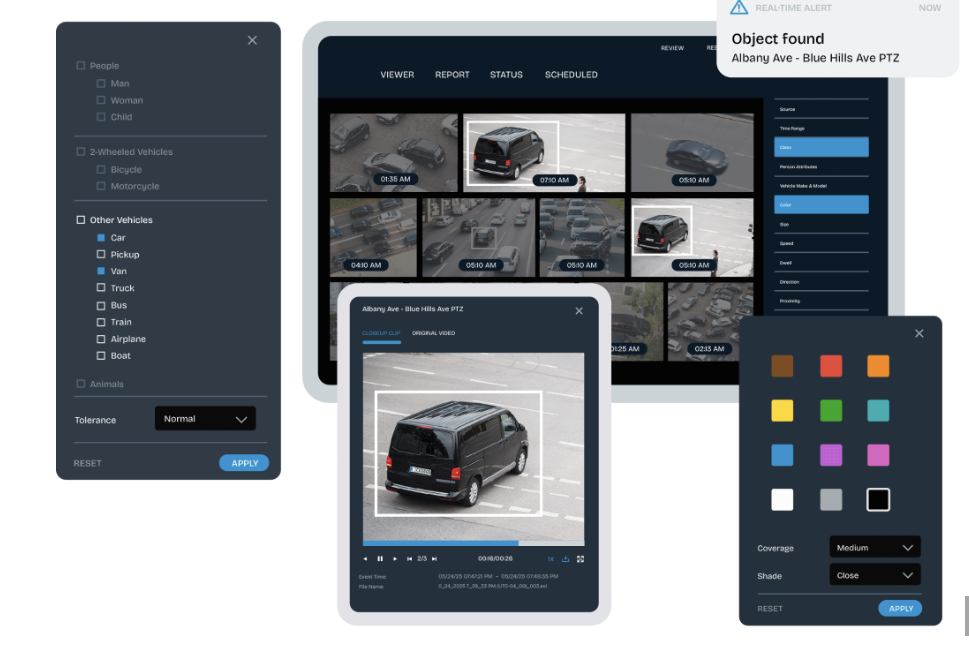
\includegraphics[width=0.6\textwidth]{briefcam.png}
    \caption{Giao diện tìm kiếm và lọc đối tượng của BriefCam~\cite{milestone2026briefcam}}
    \label{fig:briefcam}
\end{figure}

\paragraph{Liên hệ với đề tài.} BriefCam hỗ trợ tìm theo thuộc tính và theo mẫu ngoại hình, trong đó mẫu là một đối tượng chọn trong video đã ghi thay vì một ảnh tải lên từ bên ngoài như trong đề tài; tài liệu công bố không đề cập tìm kiếm bằng câu mô tả tự nhiên.

\subsection{Avigilon Appearance Search}
\label{sec:2.1.2}

Avigilon Appearance Search là công nghệ tìm kiếm video dựa trên học sâu của Avigilon, thuộc Motorola Solutions, dùng để tìm một người hay phương tiện trong nhiều giờ video trên nhiều camera~\cite{motorola2021appearance}. Người dùng có thể bắt đầu tìm kiếm bằng cách chọn đặc điểm ngoại hình từ danh sách có sẵn như màu quần áo, giới tính, nhóm tuổi; bằng cách tải lên một bức ảnh; hoặc bằng cách chọn một đối tượng trong video làm mẫu~\cite{motorola2021appearance}. Kết quả giúp lần theo lộ trình của đối tượng và có thể được đánh dấu, trích xuất thành bộ bằng chứng về diễn biến sự việc. Hình~\ref{fig:avigilon} minh họa giao diện khi đánh dấu một người. Công nghệ được tích hợp trong phần mềm quản lý video Avigilon Control Center, chạy trên camera và đầu ghi của hãng hoặc trên thiết bị Avigilon AI Appliance cho camera ONVIF của hãng khác.

\begin{figure}[H]
    \centering
    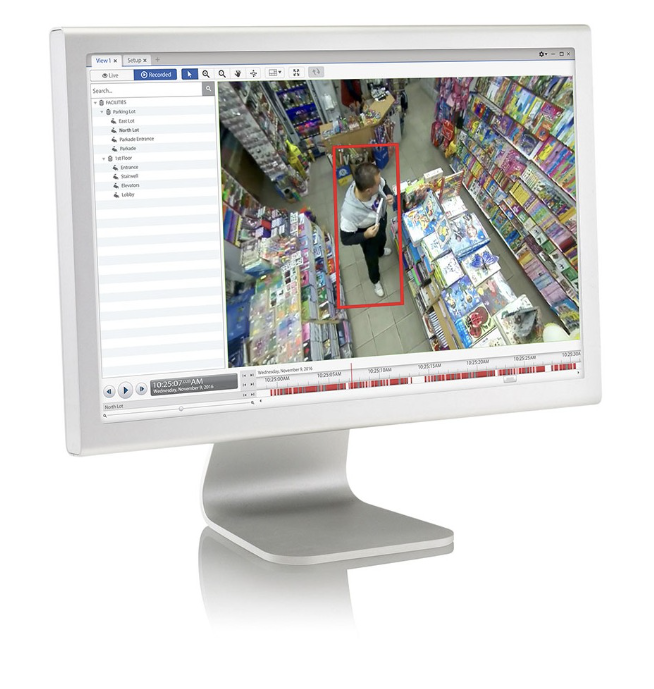
\includegraphics[width=0.45\textwidth]{avigilon.png}
    \caption{Giao diện phần mềm Avigilon Control Center với đối tượng được đánh dấu~\cite{avigilon2026appearance}}
    \label{fig:avigilon}
\end{figure}

\paragraph{Liên hệ với đề tài.} Avigilon hỗ trợ hai hình thức mô tả của đề tài là chọn thuộc tính và dùng ảnh tham chiếu, và cho phép tổng hợp kết quả thành bằng chứng, tương tự hồ sơ vụ việc của đề tài; tài liệu không đề cập tìm bằng câu mô tả tự do, và hệ thống gắn với phần mềm, thiết bị của hãng.

\subsection{Verkada AI-Powered Search}
\label{sec:2.1.3}

Verkada AI-Powered Search, giới thiệu năm 2024 trên nền tảng quản lý an ninh đám mây Command, cho phép tìm người và phương tiện bằng ngôn ngữ đời thường, ví dụ ``person wearing helmet'', thay vì chọn từ danh sách thuộc tính~\cite{verkada2024aisearch}, và tìm bằng ảnh tải lên của người, phương tiện hay đồ vật~\cite{verkada2024reverse}. Theo bài viết kỹ thuật của hãng~\cite{verkada2025scaling}, camera tạo các ảnh cắt của đối tượng; trên đám mây, ảnh cắt được mã hóa thành vector bằng mô hình CLIP, vốn đưa ảnh và văn bản vào cùng một không gian biểu diễn, và lưu vào một cơ sở dữ liệu vector; câu truy vấn được mã hóa theo cùng cách để tìm các ảnh gần nhất. Hình~\ref{fig:verkada} minh họa kết quả của một truy vấn bằng câu mô tả. Hệ thống vận hành tốt nhất với camera của Verkada; camera hãng khác kết nối qua thiết bị Command Connector với độ trễ cao hơn~\cite{verkada2024connector}.

\begin{figure}[H]
    \centering
    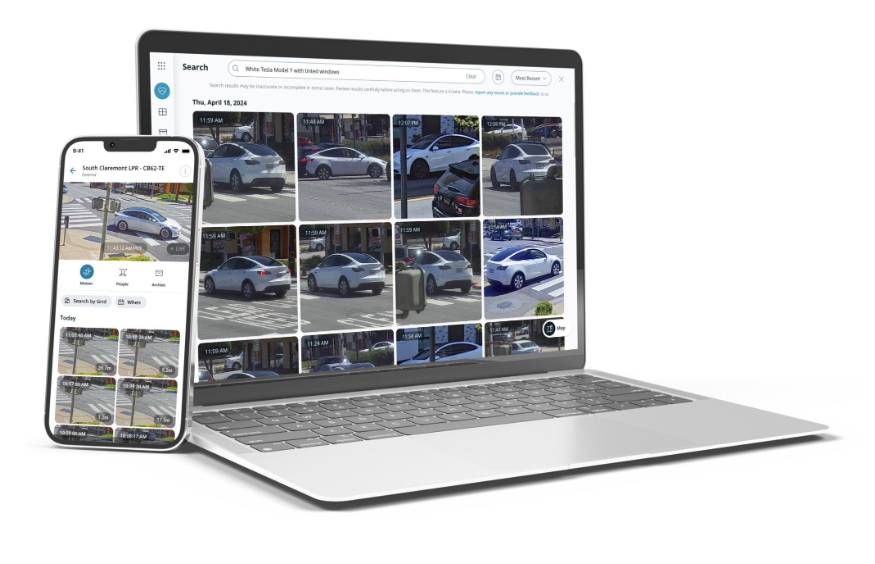
\includegraphics[width=0.52\textwidth]{verkada.png}
    \caption{Kết quả tìm kiếm bằng câu mô tả trên nền tảng Verkada Command~\cite{verkada2024aisearch}}
    \label{fig:verkada}
\end{figure}

\paragraph{Liên hệ với đề tài.} Verkada gần với đề tài nhất về kỹ thuật: cùng hỗ trợ tìm bằng câu mô tả và bằng ảnh dựa trên không gian biểu diễn chung và cơ sở dữ liệu vector. Khác biệt nằm ở mô hình triển khai: Verkada xử lý trên hạ tầng đám mây của hãng, còn đề tài triển khai tại chỗ trên máy tính phổ thông.

% !TEX root = ../../main.tex
% C2.2 — So sánh và nhận xét các hệ thống liên quan
% Chỉ dùng thông tin đã kiểm chứng ở Mục 2.1. Ô nào tài liệu của hãng không nói tới thì ghi "không đề cập", không suy đoán.
% Cột "Hệ thống của đề tài" phải khớp ứng dụng thật (chỉ 4 thuộc tính, chỉ tiếng Anh, triển khai tại chỗ trên CPU).
\section{So sánh và nhận xét các hệ thống liên quan}
\label{sec:2.2}

Bảng~\ref{tab:related-comparison} so sánh ba hệ thống đã khảo sát với hệ thống của đề tài, dựa trên tài liệu công bố của các hãng (Mục~\ref{sec:2.1}); nội dung tài liệu không nêu được ghi là ``không đề cập''.

\begin{longtable}{|>{\raggedright\arraybackslash}p{2.2cm}|>{\raggedright\arraybackslash}p{2.85cm}|>{\raggedright\arraybackslash}p{2.85cm}|>{\raggedright\arraybackslash}p{2.85cm}|>{\raggedright\arraybackslash}p{2.85cm}|}
\caption{So sánh các hệ thống tìm kiếm người trong video}\label{tab:related-comparison}\\
\hline
\textbf{Tiêu chí} & \textbf{BriefCam} & \textbf{Avigilon Appearance Search} & \textbf{Verkada AI-Powered Search} & \textbf{Hệ thống của đề tài} \\
\hline
\endfirsthead
\multicolumn{5}{l}{\textit{(tiếp theo Bảng~\ref{tab:related-comparison})}}\\
\hline
\textbf{Tiêu chí} & \textbf{BriefCam} & \textbf{Avigilon Appearance Search} & \textbf{Verkada AI-Powered Search} & \textbf{Hệ thống của đề tài} \\
\hline
\endhead
Tìm theo thuộc tính & Có: loại đối tượng, màu sắc, kích thước, tốc độ, hướng di chuyển & Có: màu quần áo, giới tính, nhóm tuổi; loại và màu xe & Có bộ lọc thuộc tính định sẵn; được mở rộng bằng tìm kiếm bằng câu mô tả & Có: giới tính, loại và màu trang phục trên, dưới, vật mang theo; được chuyển thành câu mô tả \\
\hline
Tìm theo ảnh hoặc mẫu ngoại hình & Có: chọn đối tượng mẫu trong video để tìm ngoại hình tương tự & Có: tải ảnh lên hoặc chọn mẫu trong video & Có: tải ảnh người, phương tiện hoặc đồ vật lên & Có: tải ảnh đã cắt chứa một người \\
\hline
Tìm bằng câu mô tả tự do & Không đề cập & Không đề cập & Có & Có (chỉ tiếng Anh) \\
\hline
Cơ chế so khớp được công bố & Tìm theo siêu dữ liệu và độ tương tự ngoại hình & Học sâu trên đặc trưng ngoại hình, có kết hợp đặc trưng khuôn mặt & Mã hóa ảnh cắt và câu truy vấn vào cùng một không gian biểu diễn (CLIP), tìm trên cơ sở dữ liệu vector & Mã hóa ảnh, câu mô tả và thuộc tính vào cùng một không gian biểu diễn, tìm trên cơ sở dữ liệu vector \\
\hline
Chức năng khác & Tóm tắt video (Video Synopsis), nhận diện khuôn mặt, biển số xe, cảnh báo thời gian thực, thống kê và bản đồ nhiệt & Đánh dấu và xuất kết quả thành bằng chứng, tìm kiếm trên nhiều địa điểm & Tạo cảnh báo từ câu truy vấn, quản lý tập trung trên nền tảng đám mây & Hồ sơ vụ việc, phân quyền theo vai trò và khu vực giám sát, trang tổng quan theo dõi hồ sơ vụ việc \\
\hline
Mô hình triển khai & Tại chỗ hoặc trên máy chủ đám mây & Tại chỗ, tích hợp phần mềm quản lý video của hãng & Nền tảng đám mây của hãng & Tại chỗ trên một máy tính cá nhân \\
\hline
Yêu cầu phần cứng và thiết bị & Máy chủ xử lý bắt buộc có card đồ họa NVIDIA & Camera và đầu ghi của hãng, hoặc thiết bị AI Appliance cho camera ONVIF khác hãng & Camera của hãng, hoặc thiết bị Command Connector cho camera khác hãng & Không yêu cầu card đồ họa rời; nhận luồng từ camera bất kỳ hỗ trợ RTSP \\
\hline
Hình thức cung cấp & Phần mềm thương mại & Phần mềm và thiết bị thương mại & Nền tảng dịch vụ thương mại & Ứng dụng tự phát triển, sử dụng các mô hình đã công bố \\
\hline
\end{longtable}

Từ kết quả so sánh, có thể rút ra một số nhận xét sau:
\begin{itemize}
    \item \textbf{Hỗ trợ nhiều hình thức mô tả đã trở thành xu hướng.} Cả ba hệ thống đều hỗ trợ tìm theo thuộc tính và theo ảnh hoặc mẫu ngoại hình, nhưng trong phạm vi tài liệu khảo sát, chỉ Verkada hỗ trợ tìm bằng câu mô tả tự do, một chức năng mới xuất hiện từ năm 2024. Cách tiếp cận của Verkada, mã hóa ảnh và câu truy vấn vào cùng một không gian biểu diễn rồi tìm trên cơ sở dữ liệu vector, cho phép dùng chung một cơ chế cho cả hai hình thức.
    \item \textbf{Tìm kiếm thường đi kèm công cụ tổng hợp kết quả}, như việc đánh dấu và xuất bằng chứng của Avigilon: người dùng còn cần lưu trữ và chia sẻ kết quả trong quá trình điều tra.
    \item \textbf{Các hệ thống thương mại gắn với hạ tầng của hãng}: BriefCam cần máy chủ có card đồ họa chuyên dụng, Avigilon cần phần mềm và thiết bị của hãng, Verkada vận hành trên đám mây của hãng. Chi phí và sự phụ thuộc vào nhà cung cấp là rào cản với các tổ chức nhỏ hoặc cần lưu dữ liệu tại chỗ. Các sản phẩm này cũng tích hợp nhiều chức năng ngoài tìm kiếm như cảnh báo, nhận diện khuôn mặt, biển số xe và thống kê.
\end{itemize}

% !TEX root = ../../main.tex
% C2.3 — Định hướng phát triển của hệ thống (RÚT GỌN 2026-09-29; bản cũ ở report/archive/)
% Nối các nhận xét ở 2.2 với lựa chọn của đề tài. Chương 2 đứng trước lý thuyết: chưa nêu tên mô hình (RaSa, YOLO...).
\section{Định hướng phát triển của hệ thống}
\label{sec:2.3}

Dựa trên các nhận xét tại Mục~\ref{sec:2.2}, đề tài xác định các định hướng phát triển sau:
\begin{enumerate}
    \item \textbf{Hỗ trợ đủ ba hình thức mô tả trong cùng một cơ chế tìm kiếm}: ảnh tham chiếu, câu mô tả tự do bằng tiếng Anh, và tập thuộc tính chọn sẵn. Tương tự cách tiếp cận của Verkada, cả ba được đưa về cùng một không gian biểu diễn; tập thuộc tính được chuyển thành một câu mô tả có cấu trúc nên không cần mô hình riêng cho từng thuộc tính.
    \item \textbf{Tổ chức kết quả theo từng lần xuất hiện} của một người trên một camera, sắp xếp theo mức độ phù hợp và luôn kèm khung hình gốc để người dùng tự đánh giá; hệ thống không đưa ra kết luận về danh tính (Mục~\ref{sec:1.2}).
    \item \textbf{Quản lý kết quả thành hồ sơ vụ việc}, tương tự việc tổng hợp bằng chứng của Avigilon, để người có trách nhiệm xem lại mà không cần tìm kiếm lại.
    \item \textbf{Phân quyền theo vai trò và khu vực giám sát}, tách trách nhiệm quản trị kỹ thuật, tìm kiếm và theo dõi kết quả; người tìm kiếm chỉ truy cập dữ liệu của khu vực được giao (Mục~\ref{sec:1.1}).
    \item \textbf{Triển khai tại chỗ, không phụ thuộc nhà cung cấp phần cứng}: một ứng dụng web nhận hình ảnh qua giao thức RTSP phổ biến, xử lý và lưu trữ toàn bộ dữ liệu trên một máy tính không có card đồ họa rời.
    \end{enumerate}


% !TEX root = ../../main.tex
% Chương 3 — xem mục C3 trong report/report_plan.md
\chapter{Cơ sở lý thuyết}
\label{chapter:lythuyet}

\textit{Chương này trình bày các kiến thức nền tảng của đề tài: bài toán tìm kiếm người và truy hồi đa phương thức, các kỹ thuật phát hiện và theo vết người, lấy mẫu khung hình, học biểu diễn chung ảnh-văn bản, tìm kiếm vector và giao thức truyền phát luồng camera.}

% !TEX root = ../../main.tex
% C3.1 — Bài toán tìm kiếm người và truy hồi đa phương thức (RÚT GỌN 2026-09-29; bản cũ ở report/archive/)
% Nội dung: ReID (ảnh→ảnh) và text-based person search (văn bản→ảnh); tìm theo thuộc tính; khác nhận dạng khuôn mặt;
% hướng tiếp cận của đề tài (đơn vị kết quả là track, một không gian biểu diễn chung cho ba hình thức mô tả).
\section{Bài toán tìm kiếm người và truy hồi đa phương thức}
\label{sec:3.1}

\subsection{Phát biểu bài toán}
\label{sec:3.1.1}

Cho một tập hình ảnh người được trích xuất từ video của nhiều camera, gọi là \emph{tập dữ liệu tìm kiếm} (gallery) $\mathcal{G} = \{g_1, g_2, \ldots, g_n\}$, và một \emph{truy vấn} $q$ mô tả người cần tìm, hệ thống cần xếp hạng các phần tử của $\mathcal{G}$ theo mức độ phù hợp với $q$ và trả về $k$ phần tử phù hợp nhất. Cách tiếp cận phổ biến là học một hàm biểu diễn ánh xạ truy vấn và từng phần tử vào một không gian vector, rồi đo mức độ phù hợp bằng một hàm tương đồng $s(q, g_i)$; việc tìm kiếm khi đó trở thành tìm các vector gần nhất.

Trong video giám sát, người không có sẵn dưới dạng ảnh cắt gọn như các bộ dữ liệu chuẩn mà nằm trong khung hình toàn cảnh cùng nhiều người khác, nên bài toán còn gồm bước phát hiện. Xiao và cộng sự học đồng thời phát hiện và nhận dạng~\cite{xiao2017personsearch}, còn một hướng khác tách bộ phát hiện khỏi mô hình nhận dạng~\cite{zheng2017reidwild}; đề tài theo hướng sau để thay thế độc lập từng thành phần.

\subsection{Ba hình thức truy vấn}
\label{sec:3.1.2}
\label{sec:3.1.3}
\label{sec:3.1.4}

\paragraph{Tìm bằng hình ảnh.} Khi truy vấn là một ảnh chứa người cần tìm, bài toán tương ứng với \emph{tái nhận dạng người} (Person Re-identification, ReID): xác định các ảnh thuộc cùng một người trong dữ liệu thu từ nhiều camera hoặc nhiều thời điểm~\cite{ye2022reidsurvey}. Thách thức chính là sự thay đổi góc nhìn, ánh sáng, tư thế, hiện tượng che khuất và độ phân giải thấp: cùng một người có thể trông rất khác giữa hai camera, trong khi hai người mặc giống nhau lại có thể trông rất giống nhau.

\paragraph{Tìm bằng mô tả văn bản.} Khi người dùng chỉ có lời mô tả, ví dụ ``a man wearing a black jacket and blue jeans, carrying a backpack'', bài toán là tìm kiếm người bằng văn bản (Text-Based Person Search, TBPS), được Li và cộng sự đề xuất cùng bộ dữ liệu CUHK-PEDES gồm ảnh người kèm mô tả tiếng Anh~\cite{li2017cuhkpedes}. Đây là bài toán liên phương thức: mô hình phải đưa văn bản và ảnh về cùng một không gian biểu diễn, trong khi mô tả thường mơ hồ và khác biệt giữa những người thường nằm ở chi tiết nhỏ.

\paragraph{Tìm theo thuộc tính.} Người dùng chọn thuộc tính như giới tính, loại và màu trang phục, vật mang theo. Có thể dùng một mô hình nhận dạng thuộc tính người đi bộ~\cite{wang2022parsurvey} để lọc theo nhãn, cần dữ liệu gán nhãn cho từng thuộc tính, hoặc ghép thuộc tính thành câu theo mẫu cố định rồi tìm như văn bản. Đề tài chọn cách sau để dùng chung mô hình văn bản, nên thuộc tính ảnh hưởng thứ hạng chứ không phải điều kiện lọc bắt buộc. Lựa chọn phủ định như ``không mang ba lô'' không được hỗ trợ, vì các mô hình ngôn ngữ-thị giác kiểu CLIP gặp khó khăn đáng kể với phủ định, nhiều trường hợp chỉ đạt mức ngẫu nhiên~\cite{alhamoud2025negation}.

Khác nhận dạng khuôn mặt, tìm theo ngoại hình không dựa trên sinh trắc học, vốn cần khuôn mặt rõ, mà dựa trên trang phục, màu sắc và vật dụng, dễ thấy từ camera cao và xa nhưng có thể thay đổi và trùng giữa nhiều người. Kết quả vì vậy là gợi ý để đánh giá, không phải kết luận về danh tính.

\subsection{Hướng tiếp cận của đề tài}
\label{sec:3.1.6}

Bảng~\ref{tab:query-modes} tóm tắt ba hình thức truy vấn và cách đề tài xử lý.

\begin{table}[H]
\centering
\caption{Ba hình thức mô tả người cần tìm và cách xử lý trong đề tài}
\label{tab:query-modes}
\begin{tabularx}{\textwidth}{|>{\raggedright\arraybackslash}p{2.6cm}|L|L|L|}
\hline
\textbf{Hình thức} & \textbf{Đầu vào} & \textbf{Ưu điểm và thách thức} & \textbf{Cách xử lý trong đề tài} \\
\hline
Ảnh tham chiếu (ReID) & Ảnh đã cắt chứa một người & Giàu thông tin thị giác; nhạy với góc nhìn, ánh sáng, che khuất & Mã hóa bằng bộ mã hóa ảnh \\
\hline
Mô tả văn bản (TBPS) & Câu mô tả tiếng Anh & Không cần ảnh; mô tả có thể mơ hồ, thiếu chi tiết & Mã hóa bằng bộ mã hóa văn bản \\
\hline
Thuộc tính & Giới tính, loại và màu trang phục trên, dưới, vật mang theo & Dễ nhập, rõ ràng; chỉ diễn đạt được các thuộc tính có sẵn & Chuyển thành câu tiếng Anh có cấu trúc, rồi xử lý như mô tả văn bản \\
\hline
\end{tabularx}
\end{table}

\begin{itemize}
    \item \textbf{Một không gian biểu diễn chung.} RaSa~\cite{bai2023rasa} mã hóa ảnh và văn bản vào cùng một không gian vector, nên ảnh người, ảnh truy vấn, câu mô tả và câu từ thuộc tính so sánh trực tiếp được (Mục~\ref{sec:3.5}).
    \item \textbf{Đơn vị kết quả là một lần xuất hiện.} Người được phát hiện và theo vết (Mục~\ref{sec:3.2} và~\ref{sec:3.3}); mỗi lần xuất hiện liên tục trên một camera (track) có một khung hình đại diện và một vector, giảm số phần tử cần so khớp và tránh kết quả trùng.
    \item \textbf{Hai giai đoạn tách biệt.} Lập chỉ mục chạy nền và lưu đặc trưng; truy vấn chỉ mã hóa mô tả và tìm các vector gần nhất (Mục~\ref{sec:3.6}).
    \item \textbf{Con người ra quyết định cuối cùng.} Hệ thống chỉ xếp hạng; người dùng đánh giá từng kết quả trên hình ảnh gốc trước khi lưu.
\end{itemize}

% !TEX root = ../../main.tex
% C3.2 — Phát hiện người trong ảnh (RÚT GỌN 2026-09-29; bản cũ ở report/archive/)
% Nguyên lý; lý do chọn YOLO11n so với phương án khác để ở Mục 6.1.4.
% Khớp app: config/ultralytics_yolo_detector.json (conf 0.1 = track_low_threshold của ByteTrack, iou 0.7, max 300), chỉ lớp person, confidence chỉ dùng nội bộ.
\section{Phát hiện người trong ảnh}
\label{sec:3.2}

\subsection{Bài toán phát hiện đối tượng}
\label{sec:3.2.1}

Phát hiện đối tượng (object detection) xác định vị trí và loại của các đối tượng trong một ảnh. Với mỗi đối tượng, mô hình trả về một \emph{khung bao} (bounding box) hình chữ nhật, thường biểu diễn bằng tọa độ hai góc $(x_1, y_1, x_2, y_2)$, \emph{lớp} của đối tượng và một \emph{độ tin cậy} (confidence score). Hai khung bao được so sánh bằng chỉ số giao trên hợp (Intersection over Union, IoU):
\begin{equation}
    \mathrm{IoU}(A, B) = \frac{|A \cap B|}{|A \cup B|},
    \label{eq:iou}
\end{equation}
nhận giá trị từ 0 khi hai khung không giao nhau đến 1 khi trùng khít. IoU được dùng khi loại bỏ các dự đoán trùng lặp và khi liên kết phát hiện giữa các khung hình trong bài toán theo vết (Mục~\ref{sec:3.3}).

\subsection{Hướng tiếp cận hai giai đoạn và một giai đoạn}
\label{sec:3.2.2}

Mô hình \emph{hai giai đoạn} như Faster R-CNN~\cite{ren2017fasterrcnn} trước tiên dùng một mạng đề xuất vùng để sinh các vùng có khả năng chứa đối tượng, sau đó phân loại từng vùng và tinh chỉnh khung bao; cách này chính xác nhưng tốn kém do phải xử lý nhiều vùng đề xuất. Mô hình \emph{một giai đoạn} như YOLO (You Only Look Once)~\cite{redmon2016yolo} xem phát hiện là một bài toán hồi quy duy nhất, dự đoán trực tiếp khung bao và lớp của mọi đối tượng trong một lần lan truyền qua ảnh, nên nhanh hơn đáng kể và phù hợp với việc xử lý nhiều khung hình video.

\subsection{Họ mô hình YOLO}
\label{sec:3.2.3}

Các mô hình YOLO hiện đại gồm ba phần: phần trích xuất đặc trưng (backbone) ở nhiều mức chi tiết, phần kết hợp đặc trưng (neck) ở nhiều tỉ lệ để phát hiện được cả đối tượng lớn gần camera lẫn đối tượng nhỏ ở xa, và phần dự đoán (head) cho khung bao, lớp và độ tin cậy. YOLO11 do Ultralytics phát hành năm 2024 với năm kích cỡ (n, s, m, l, x) để đánh đổi giữa tốc độ và độ chính xác~\cite{ultralytics2024yolo11docs}. Các mô hình được huấn luyện sẵn trên COCO~\cite{lin2014coco}, gồm 80 lớp đối tượng thông dụng trong đó có lớp \emph{người}, nên dùng được trực tiếp để phát hiện người mà không cần huấn luyện thêm.

\subsection{Hậu xử lý: ngưỡng tin cậy và loại bỏ trùng lặp}
\label{sec:3.2.4}

Đầu ra thô có nhiều khung độ tin cậy thấp và nhiều khung chồng lấn. Khung dưới ngưỡng tin cậy bị loại, và phép loại bỏ khung không cực đại (Non-Maximum Suppression, NMS) giữ khung tin cậy nhất, bỏ các khung cùng lớp chồng lấn với nó quá ngưỡng IoU. Ngưỡng tin cậy thấp ít bỏ sót nhưng thêm phát hiện sai; ngưỡng IoU thấp loại chồng lấn mạnh hơn nhưng có thể gộp nhầm người đứng sát nhau.

\subsection{Vai trò của bước phát hiện trong hệ thống}
\label{sec:3.2.5}

Mô hình phát hiện được áp dụng lên các khung hình đã được lấy mẫu (Mục~\ref{sec:3.4}) và chỉ giữ lớp \emph{người}, với ngưỡng tin cậy 0,1, ngưỡng IoU của NMS 0,7 và tối đa 300 phát hiện trên một khung hình. Ngưỡng thấp là chủ ý: ByteTrack cần các phát hiện độ tin cậy thấp, thường là người bị che khuất một phần, để giữ track (Mục~\ref{sec:3.3}); chúng không khởi tạo track, và track cần hai lần quan sát mới được xác nhận, nên phần lớn phát hiện sai thoáng qua bị loại ở bước theo vết. Lý do chọn YOLO11n được trình bày tại Mục~\ref{sec:6.1.4}.

% !TEX root = ../../main.tex
% C3.3 — Theo vết nhiều đối tượng (RÚT GỌN 2026-09-29; bản cũ ở report/archive/)
% Nguyên lý; lý do chọn ByteTrack/BoT-SORT để ở Mục 6.1.4.
% Khớp app: config/bytetrack_tracker.json và botsort_tracker.json (cùng ngưỡng: high 0,25, low 0,1, new 0,25,
% match 0,8, fuse_score, xác nhận sau 2 lần quan sát, kết thúc khi mất dấu > 3 khung hình được xử lý hoặc > 2000 ms).
% Mốc thời gian: tệp video dùng PTS (workers/sources/file.py); RTSP dùng đồng hồ lúc worker đọc khung (workers/sources/rtsp.py)
% -> phụ thuộc tốc độ xử lý (architect §13 #7, chưa sửa).
\section{Theo vết nhiều đối tượng}
\label{sec:3.3}

\subsection{Bài toán và các thành phần cơ bản}
\label{sec:3.3.1}
\label{sec:3.3.2}

Mô hình phát hiện xử lý từng khung hình độc lập nên không biết một người có phải người đã thấy trước đó. Theo vết nhiều đối tượng (Multi-Object Tracking, MOT) gán cho mỗi đối tượng một mã giữ qua các khung hình; chuỗi khung bao của nó là một \emph{track}, trong đề tài trở thành một \emph{lần xuất hiện}, đơn vị kết quả tìm kiếm (Mục~\ref{sec:3.1.6}).

Hướng phổ biến là \emph{theo vết dựa trên phát hiện} (tracking-by-detection), với nền tảng là thuật toán SORT~\cite{bewley2016sort} gồm ba thành phần. Thứ nhất, mỗi track gắn với một bộ lọc Kalman~\cite{kalman1960} dự đoán vị trí và kích thước khung bao ở khung hình hiện tại theo giả định chuyển động gần như đều, rồi được hiệu chỉnh bằng phát hiện thực tế. Thứ hai, mức độ khớp giữa track và phát hiện được đo bằng IoU (Công thức~\ref{eq:iou}) giữa khung bao dự đoán và khung bao phát hiện. Thứ ba, việc gán mỗi phát hiện cho tối đa một track với tổng chi phí nhỏ nhất được giải bằng thuật toán Hungary~\cite{kuhn1955hungarian}; phát hiện chưa được ghép có thể khởi tạo track mới, còn track chưa được ghép được xem là đang mất dấu.

\subsection{Thuật toán ByteTrack}
\label{sec:3.3.3}

Các phương pháp trước loại bỏ phát hiện độ tin cậy thấp, nên người bị che khuất một phần dễ bị đứt track. ByteTrack~\cite{zhang2022bytetrack} liên kết hai bước: phát hiện độ tin cậy cao được ghép trước với mọi track, rồi các track còn lại ghép với phát hiện độ tin cậy thấp, nhờ đó người bị che khuất vẫn giữ track; phát hiện thấp không ghép được bị loại vì phần lớn là nền. Chỉ phát hiện độ tin cậy cao khởi tạo track, và track mất dấu được giữ thêm một lúc để nối lại.

\subsection{Thuật toán BoT-SORT}
\label{sec:3.3.4}

BoT-SORT~\cite{aharon2022botsort} mở rộng ByteTrack bằng cách điều chỉnh trạng thái của bộ lọc Kalman, bù chuyển động của camera và kết hợp đặc trưng tái nhận dạng ngoại hình (ReID) vào bước liên kết. Trong đề tài, BoT-SORT là thuật toán thay thế với cùng các ngưỡng như ByteTrack; bù chuyển động camera và ReID được tắt vì camera cố định và để giữ chi phí thấp trên máy chỉ có CPU.

\subsection{Vòng đời track trong hệ thống}
\label{sec:3.3.5}

Thuật toán theo vết nhận các phát hiện trên những khung hình đã được lấy mẫu, riêng cho từng camera, với các quy tắc sau:
\begin{itemize}
    \item \textbf{Ngưỡng độ tin cậy:} phát hiện từ 0,25 trở lên được xem là cao và có thể khởi tạo track mới; phát hiện từ 0,1 đến dưới 0,25 chỉ dùng trong bước liên kết thứ hai.
    \item \textbf{Xác nhận:} track chỉ được xác nhận sau ít nhất hai lần quan sát; track chưa xác nhận không tạo ra kết quả.
    \item \textbf{Kết thúc:} track kết thúc khi mất dấu quá ba khung hình xử lý liên tiếp hoặc quá hai giây không quan sát, hoặc khi luồng kết thúc. Cả tệp video lẫn luồng RTSP đều dùng dấu thời gian ghi trong chính luồng (Mục~\ref{sec:3.7.4}), nên quy tắc đo thời gian đã trôi qua trước camera và không phụ thuộc tốc độ xử lý của máy.
    \item \textbf{Phạm vi mã định danh:} chỉ trong một camera và một phiên xử lý; hệ thống không liên kết track của cùng một người giữa nhiều camera.
\end{itemize}

% !TEX root = ../../main.tex
% C3.4 — Lấy mẫu khung hình (RÚT GỌN 2026-09-29: một mục ngắn, không chia tiểu mục; bản cũ ở report/archive/)
% Khớp app: workers/sampling.py (giữ khung có chỉ số i với i mod N = 0; profile baseline N=10, throughput N=20 mặc định);
% lấy mẫu sau bước giải mã. Video WILDTRACK 59,94 fps. Số đo so sánh N ở Mục 8.5.
\section{Lấy mẫu khung hình}
\label{sec:3.4}
\label{sec:3.4.3}

Video giám sát thường có vài chục khung hình mỗi giây; video của bộ dữ liệu trong đề tài có khoảng 60 khung hình mỗi giây, nên hai khung hình liên tiếp chỉ cách nhau khoảng 17 mili giây và gần như giống hệt nhau. Chạy các mô hình trên mọi khung hình vì vậy rất tốn kém mà mang lại ít thông tin mới. Đề tài lấy mẫu đều theo chỉ số khung hình: với chỉ số $i$ và khoảng lấy mẫu $N$, khung hình được chọn khi và chỉ khi
\begin{equation}
    i \bmod N = 0,
    \label{eq:sampling}
\end{equation}
và vẫn giữ nguyên chỉ số cùng mốc thời gian gốc, để thời điểm xuất hiện của người được xác định theo đúng dòng thời gian của camera. Với nguồn $f$ khung hình mỗi giây, hai khung hình được xử lý cách nhau $N/f$ giây: khoảng 0,17 giây với $N = 10$ và 0,33 giây với $N = 20$.

Khoảng lấy mẫu là một đánh đổi. Lấy mẫu đứng trước mô hình phát hiện nên số lần chạy các mô hình AI giảm khoảng $N$ lần; riêng bước giải mã vẫn phải thực hiện trên mọi khung hình, vì phần lớn khung hình H.264 chỉ giải mã được khi đã giải mã các khung trước đó (Mục~\ref{sec:3.7.1}). Ngược lại, $N$ càng lớn thì người xuất hiện quá ngắn càng dễ bị bỏ sót, vì track cần ít nhất hai lần quan sát, và người di chuyển càng xa giữa hai lần quan sát, khiến việc liên kết theo IoU khó hơn và track dễ bị đứt. Hệ thống cung cấp hai cấu hình định sẵn: \emph{baseline} với $N = 10$ ưu tiên chất lượng track, và \emph{throughput} với $N = 20$ ưu tiên tốc độ, được chọn làm mặc định dựa trên đo đạc trên máy triển khai (Mục~\ref{sec:8.5}). Mỗi công việc lưu lại giá trị $N$ đã dùng để kết quả có thể được đối chiếu và tái lập.

% !TEX root = ../../main.tex
% C3.5 — Học biểu diễn chung ảnh--văn bản (RÚT GỌN 2026-09-29; bản cũ ở report/archive/)
% Nguồn: RaSa (bai2023rasa, IJCAI 2023) — đã đọc toàn văn; CLIP (radford2021clip); ALBEF (li2021albef).
% Khớp app: config/rasa_cuhk_pedes_runtime.json (image_size 384, embedding_dimension 256, l2_normalized,
% itm_rerank_supported true, itm_rerank_top_k 128) ; ai/encoders/rasa.py ; rerank mặc định TẮT (AIW-15).
\section{Học biểu diễn chung ảnh-văn bản}
\label{sec:3.5}

\subsection{Không gian biểu diễn chung và học tương phản}
\label{sec:3.5.1}
\label{sec:3.5.2}

Để so sánh một câu mô tả với một ảnh người, hệ thống dùng hai bộ mã hóa (encoder): bộ mã hóa ảnh biến ảnh thành một vector đặc trưng, bộ mã hóa văn bản biến câu thành một vector cùng số chiều. Hai bộ mã hóa được huấn luyện sao cho vector của một ảnh và của câu mô tả đúng ảnh đó nằm gần nhau, còn các cặp không tương ứng nằm xa nhau; không gian có tính chất này gọi là \emph{không gian biểu diễn chung} (joint embedding space). Mức độ gần nhau được đo bằng độ tương đồng cosine
\begin{equation}
    s(\mathbf{u}, \mathbf{v}) = \frac{\mathbf{u}^\top \mathbf{v}}{\lVert \mathbf{u} \rVert \, \lVert \mathbf{v} \rVert},
    \label{eq:cosine}
\end{equation}
trở thành tích vô hướng $\mathbf{u}^\top \mathbf{v}$ khi các vector đã được chuẩn hóa độ dài bằng 1 (chuẩn hóa L2). Ưu điểm quan trọng là ảnh trong kho chỉ cần mã hóa một lần khi lập chỉ mục; khi truy vấn, hệ thống chỉ mã hóa truy vấn rồi so sánh với các vector đã có (Mục~\ref{sec:3.1.6}).

Phương pháp huấn luyện phổ biến là \emph{học tương phản} (contrastive learning): trong mỗi nhóm $B$ cặp ảnh-văn bản, câu đúng của một ảnh là mẫu dương, $B-1$ câu còn lại là mẫu âm, và hàm mất mát
\begin{equation}
    \mathcal{L}_i = -\log \frac{\exp\left(s(\mathbf{v}_i, \mathbf{t}_i)/\tau\right)}{\sum_{j=1}^{B} \exp\left(s(\mathbf{v}_i, \mathbf{t}_j)/\tau\right)}
    \label{eq:contrastive}
\end{equation}
khuyến khích độ tương đồng với mẫu dương cao hơn hẳn các mẫu âm, với $\tau$ là tham số nhiệt độ; chiều từ câu đến ảnh được tính tương tự. CLIP~\cite{radford2021clip} áp dụng cách học này trên khoảng 400 triệu cặp ảnh-văn bản từ Internet. ALBEF~\cite{li2021albef} trước tiên căn chỉnh biểu diễn của hai phương thức bằng học tương phản, rồi kết hợp chúng trong một bộ mã hóa đa phương thức dùng cơ chế chú ý chéo (cross-attention) để so khớp chi tiết từng từ với từng vùng ảnh.

\subsection{Mô hình RaSa}
\label{sec:3.5.3}

Mô hình tổng quát như CLIP và ALBEF khó phân biệt những khác biệt nhỏ giữa người có ngoại hình tương tự, chẳng hạn cùng áo khoác nhưng khác màu quần. RaSa (Relation and Sensitivity Aware representation learning)~\cite{bai2023rasa} được xây dựng trên nền ALBEF và thiết kế riêng cho tìm kiếm người bằng văn bản, gồm bộ mã hóa ảnh 12 lớp transformer, bộ mã hóa văn bản 6 lớp và bộ mã hóa đa phương thức 6 lớp. Ba điểm chính của RaSa:
\begin{itemize}
    \item \textbf{Học tương phản trong và giữa các phương thức.} Ngoài ghép ảnh với câu, các ảnh của cùng một người cũng được kéo lại gần nhau. Tính chất này làm vector của hai ảnh cùng một người nằm gần nhau, là cơ sở để đề tài dùng cùng không gian vector cho truy vấn bằng ảnh.
    \item \textbf{Học nhận biết quan hệ.} Mỗi câu mô tả được viết cho \emph{một} ảnh cụ thể và có thể không hoàn toàn đúng với các ảnh khác của cùng người đó; RaSa phân biệt hai loại cặp dương này để không học những chi tiết không đúng.
    \item \textbf{Học nhạy với thay đổi.} Mô hình được huấn luyện để nhận ra khi một từ quan trọng, như ``áo đỏ'' thành ``áo xanh'', bị thay, làm thay đổi ý nghĩa của câu.
\end{itemize}
Khi truy vấn, RaSa có thể xếp hạng lại 128 kết quả đầu bằng bộ mã hóa đa phương thức để tăng độ chính xác, nhưng cách này tốn kém hơn nhiều so với chỉ so sánh vector. Trên tập kiểm tra của CUHK-PEDES, RaSa đạt Rank-1 là 76,51\% và mAP là 69,38\%~\cite{bai2023rasa}.

\subsection{Sử dụng RaSa trong hệ thống}
\label{sec:3.5.4}

Hệ thống dùng trọng số RaSa đã huấn luyện sẵn trên CUHK-PEDES, không huấn luyện lại. Bộ mã hóa ảnh mã hóa ảnh người cắt từ khung hình đại diện khi lập chỉ mục và ảnh truy vấn khi tìm bằng ảnh, với ảnh đầu vào được đưa về $384 \times 384$ điểm ảnh; bộ mã hóa văn bản mã hóa câu mô tả và câu sinh từ thuộc tính. Vector có 256 chiều, đã chuẩn hóa L2, nên cả ba kiểu truy vấn được so sánh với cùng một tập vector bằng tích vô hướng, và mỗi track chỉ cần một vector. Bước xếp hạng lại không được bật, vì chỉ áp dụng cho truy vấn văn bản, tốn kém trên máy chỉ có CPU, và chưa có số đo cho thấy nó cải thiện kết quả trên dữ liệu của đề tài.

Cần lưu ý hai điểm. Thứ nhất, RaSa được thiết kế và đánh giá cho tìm kiếm bằng văn bản; dùng bộ mã hóa ảnh của nó cho truy vấn ảnh-ảnh là lựa chọn của đề tài dựa trên tính chất học tương phản trong cùng phương thức, không phải kết quả đã được công bố. Thứ hai, CUHK-PEDES được xây dựng từ ảnh của năm bộ dữ liệu tái nhận dạng người có sẵn~\cite{li2017cuhkpedes}, mỗi ảnh là một người đã được cắt gọn kèm câu mô tả viết riêng cho ảnh đó; còn ảnh người trong đề tài được cắt tự động từ khung hình toàn cảnh của một khu vực đông người, với bối cảnh và góc quay khác, và thường bị người xung quanh che khuất một phần. Sự khác biệt về miền dữ liệu (domain gap) này ảnh hưởng trực tiếp đến chất lượng truy vấn bằng văn bản và thuộc tính (Mục~\ref{sec:8.4}).

% !TEX root = ../../main.tex
% C3.6 — Tìm kiếm vector (RÚT GỌN 2026-09-29; bản cũ ở report/archive/)
% Nguồn: HNSW (malkov2020hnsw, TPAMI 42(4)); Milvus (wang2021milvus, SIGMOD 2021); tài liệu Milvus HNSW + filtered search.
% Khớp app: storage/milvus/vectors.py (HNSW, IP, M=16, efConstruction=128, ef=64; filter area + READY + camera_ids + khoảng thời gian);
% services/track_search.py (top_k ∈ {4,8,12,16}; đối chiếu PostgreSQL, bỏ kết quả không hợp lệ, nhân đôi limit, tối đa 3 vòng → limit ≤ 64 = ef).
\section{Tìm kiếm vector}
\label{sec:3.6}

\subsection{Tìm kiếm lân cận gần nhất và chỉ mục HNSW}
\label{sec:3.6.1}
\label{sec:3.6.2}

Khi mỗi lần xuất hiện được đại diện bởi một vector (Mục~\ref{sec:3.5}) và truy vấn cũng được mã hóa thành một vector $\mathbf{q}$, việc tìm kiếm trở thành bài toán \emph{tìm $k$ lân cận gần nhất}: trong $n$ vector đã lưu, tìm $k$ vector có tích vô hướng với $\mathbf{q}$ lớn nhất, tương đương độ tương đồng cosine khi vector đã chuẩn hóa. Tìm kiếm vét cạn luôn chính xác nhưng chi phí tăng tuyến tính theo $n$, nên thời gian phản hồi tăng dần khi dữ liệu tích lũy. \emph{Tìm kiếm lân cận gần nhất gần đúng} (Approximate Nearest Neighbor, ANN) xây dựng trước một chỉ mục để khi truy vấn chỉ cần xét một phần nhỏ dữ liệu, chấp nhận bỏ sót một phần nhỏ lân cận thực sự để đổi lấy tốc độ.

HNSW (Hierarchical Navigable Small World)~\cite{malkov2020hnsw} là phương pháp ANN dựa trên đồ thị: mỗi vector là một đỉnh nối với một số vector gần nó, và việc tìm kiếm lặp lại việc di chuyển sang đỉnh kề gần truy vấn hơn. Các đỉnh được tổ chức thành nhiều tầng, tầng trên thưa để di chuyển nhanh tới vùng gần truy vấn, tầng dưới cùng chứa mọi vector để tìm chính xác trong vùng đó, nên độ phức tạp tìm kiếm tăng theo hàm logarit của số phần tử~\cite{malkov2020hnsw}. Chỉ mục có ba tham số chính~\cite{milvus2026hnsw}: số cạnh tối đa của mỗi đỉnh $M$ và số ứng viên khi xây dựng chỉ mục \textit{ef\-Con\-struc\-tion}, càng lớn thì đồ thị càng tốt nhưng tốn bộ nhớ và thời gian xây dựng hơn; và số ứng viên khi tìm kiếm $\mathit{ef}$, càng lớn thì càng chính xác nhưng chậm hơn, và không nên nhỏ hơn số kết quả cần lấy.

\subsection{Tìm kiếm vector kết hợp điều kiện lọc}
\label{sec:3.6.3}

Truy vấn trong hệ thống giám sát thường kèm điều kiện, như chỉ trong khu vực của người dùng hay trong một khoảng thời gian. Với cách \textbf{lọc sau}, hệ thống lấy $k$ vector gần nhất trên toàn bộ dữ liệu rồi mới loại những kết quả không thỏa điều kiện, nên có thể trả về ít hơn $k$ kết quả, thậm chí không có kết quả nào, khi khu vực của người dùng chỉ chiếm một phần nhỏ dữ liệu. Với cách \textbf{lọc trước}, hệ thống xác định tập vector thỏa điều kiện rồi chỉ tìm trong tập đó, nên mọi kết quả đều thuộc phạm vi được phép và chỉ ít hơn $k$ khi phạm vi thực sự có ít dữ liệu. Milvus~\cite{wang2021milvus}, hệ quản trị cơ sở dữ liệu vector mã nguồn mở, lưu các trường vô hướng bên cạnh vector và thực hiện tìm kiếm theo cách lọc trước~\cite{milvus2026filtered}.

\subsection{Tìm kiếm vector trong hệ thống}
\label{sec:3.6.4}

Hệ thống dùng Milvus với chỉ mục HNSW, độ đo tích vô hướng, $M = 16$, \textit{ef\-Con\-struc\-tion}~$= 128$ và $\mathit{ef} = 64$. Một lượt tìm kiếm gửi cho Milvus vector truy vấn cùng điều kiện lọc gồm khu vực của người dùng, tập camera được phép, khoảng thời gian nếu có và trạng thái sẵn sàng, rồi nhận về tối đa $k$ kết quả với $k \in \{4, 8, 12, 16\}$. Độ tương đồng được hiển thị dưới dạng điểm phù hợp và chỉ được tính khi truy vấn. Mỗi kết quả được đối chiếu với PostgreSQL để lấy thông tin chi tiết và kiểm tra lại phạm vi quyền; kết quả không còn hợp lệ do hai kho tạm thời chưa đồng bộ bị loại, và nếu còn ít hơn $k$ kết quả, hệ thống tìm lại với số lượng gấp đôi, tối đa ba lượt, nên số lượng cần lấy không vượt quá 64, bằng giá trị $\mathit{ef}$. Với lượng dữ liệu trình diễn của đề tài (1.523 track, Mục~\ref{sec:7.2}), tìm kiếm vét cạn vẫn đủ nhanh; chỉ mục HNSW được chọn để giữ thời gian phản hồi khi dữ liệu tích lũy từ nhiều camera trong thời gian dài.

% !TEX root = ../../main.tex
% C3.7 — Giao thức RTSP và giả lập luồng camera (RÚT GỌN 2026-09-29; bản cũ ở report/archive/)
% Nguồn: RFC 2326 (RTSP 1.0), RFC 7826 (RTSP 2.0, bỏ RECORD/ANNOUNCE), RFC 3550 (RTP), RFC 6184 (RTP payload H.264, đồng hồ 90 kHz),
% Wiegand 2003 (H.264), tài liệu FFmpeg (-re, -stream_loop, stream copy), MediaMTX.
% Khớp app: scripts/rtsp.ps1 (FFmpeg -re -stream_loop -1 -i camN.mp4 -c copy -f rtsp -rtsp_transport tcp); workers/sources/rtsp.py (PyAV, tcp,
% timeout kết nối/đọc 8 s, kết nối lại tối đa 3 lần, chờ 0,25 s nhân đôi đến 2 s, mốc thời gian theo đồng hồ worker).
\section{Giao thức RTSP và giả lập luồng camera}
\label{sec:3.7}

\subsection{Video nén H.264}
\label{sec:3.7.1}

Camera IP mã hóa hình ảnh thành video nén trước khi truyền, vì một khung hình 1920$\times$1080 chưa nén chiếm khoảng 6~MB, tức khoảng 370~MB mỗi giây ở 60 khung hình mỗi giây. H.264~\cite{wiegand2003h264} là chuẩn nén phổ biến của camera giám sát và cũng là định dạng video của đề tài. \emph{Khung I} chỉ dùng dự đoán trong chính khung hình nên giải mã được độc lập; \emph{khung P} và \emph{khung B} chỉ lưu dịch chuyển và phần sai khác so với khung tham chiếu, nên chỉ giải mã được khi đã có khung tham chiếu. Vì vậy bước giải mã phải thực hiện trên mọi khung hình dù hệ thống chỉ phân tích một phần (Mục~\ref{sec:3.4}), và một bộ giải mã bắt đầu nhận luồng giữa chừng phải đợi tới khung I kế tiếp.

\subsection{Giao thức RTSP và RTP}
\label{sec:3.7.2}

RTSP (Real Time Streaming Protocol)~\cite{rfc2326} là giao thức \emph{điều khiển}: phía nhận xác định luồng bằng một địa chỉ dạng \texttt{rtsp://<máy chủ>:<cổng>/<đường dẫn>} và trao đổi các lệnh \texttt{DESCRIBE}, \texttt{SETUP}, \texttt{PLAY}, \texttt{TEARDOWN} để lấy mô tả, thiết lập, bắt đầu và kết thúc phiên. Dữ liệu được mang bởi RTP (Real-time Transport Protocol)~\cite{rfc3550}: video nén được chia thành các gói có số thứ tự và dấu thời gian; với H.264, dấu thời gian dùng đồng hồ 90~kHz~\cite{rfc6184}. Gói RTP có thể gửi qua UDP, độ trễ thấp nhưng có thể mất gói, hoặc xen kẽ trên kết nối TCP của phiên RTSP, không mất gói nhưng có thể đến chậm khi nghẽn. RTSP 2.0~\cite{rfc7826} đã bỏ các lệnh dùng để đẩy luồng lên máy chủ, nên các công cụ giả lập của đề tài dùng phiên bản 1.0.

\subsection{Giả lập camera bằng máy chủ phát luồng}
\label{sec:3.7.3}

Để hệ thống được kiểm tra với đúng giao thức của camera IP, mỗi tệp video được phát lại thành một luồng RTSP đóng vai trò một camera. Máy chủ phát luồng MediaMTX~\cite{mediamtx2026} cho phép đẩy luồng lên và đọc luồng xuống qua RTSP, mỗi luồng ở một đường dẫn riêng như \texttt{/cam1}. Công cụ FFmpeg~\cite{ffmpeg2026docs} đọc tệp và đẩy lên MediaMTX với ba tùy chọn: \texttt{-re} để phát theo đúng tốc độ khung hình gốc, \texttt{-stream\_loop -1} để lặp vô hạn như camera chạy liên tục, và \texttt{-c copy} để sao chép nguyên dữ liệu nén mà không mã hóa lại, nên luồng mang đúng dữ liệu H.264 của tệp gốc và gần như không tốn tài nguyên. Luồng giả lập giống camera thật ở chỗ cùng giao thức, cùng định dạng và \emph{không chờ} phía nhận: nếu phía nhận xử lý chậm, dữ liệu mới vẫn tiếp tục được phát. Khác biệt là nội dung lặp theo chu kỳ và hầu như không có mất gói hay mất kết nối như mạng camera thực tế.

\subsection{Tiếp nhận luồng RTSP trong hệ thống}
\label{sec:3.7.4}

Tiến trình xử lý nền đọc luồng qua thư viện PyAV, vốn dùng các thư viện giải mã của FFmpeg, với dữ liệu RTP xen kẽ trên TCP để tránh mất gói làm hỏng ảnh. Việc kết nối và chờ dữ liệu đều giới hạn 8 giây; khi luồng gián đoạn, hệ thống thử kết nối lại tối đa ba lần với thời gian chờ tăng dần từ 0,25 giây đến 2 giây, sau đó ghi nhận lượt xử lý là lỗi. Mỗi khung hình được gắn mốc thời gian theo thời điểm hệ thống nhận được, thay vì dấu thời gian RTP của luồng (Mục~\ref{sec:3.3.5}). Vì tốc độ xử lý chậm hơn nhiều so với tốc độ phát, hệ thống không thể phân tích liên tục mọi camera; cách phân chia thời gian xử lý giữa các camera được trình bày ở Mục~\ref{sec:5.2.1}.


% !TEX root = ../../main.tex
% Chương 4 — xem mục C4 trong report/report_plan.md
\chapter{Phân tích hệ thống}
\label{chapter:phantich}

\textit{Chương này phân tích các yêu cầu của hệ thống: tác nhân, yêu cầu chức năng và phi chức năng, mô hình use case và ma trận phân quyền.}

% !TEX root = ../../main.tex
% C4.1 — Các tác nhân của hệ thống
% Nguồn: project_requirements.md mục 1–4 (+ quy ước thuật ngữ giao diện); usecase_detail.md UC-01, UC-02 (A1: Admin chỉ gán vai trò Operator/Viewer);
% architect.md mục 2 (vai trò và chức năng), mục 5 (khu vực, owner Case, đổi khu vực).
% Đây là nơi ĐẦU TIÊN nêu tên vai trò: Quản trị viên (Admin), Giám sát viên (Operator), Quản lý (Viewer); Case = vụ việc.
% Tài khoản Admin khởi tạo khi triển khai (backend plan: bootstrap Admin qua seed/CLI) — không có chức năng tạo Admin trên giao diện.
\section{Các tác nhân của hệ thống}
\label{sec:4.1}

Hệ thống có ba tác nhân, tương ứng với ba loại tài khoản người dùng được phân chia theo trách nhiệm: \textbf{Quản trị viên} (Admin), \textbf{Giám sát viên} (Operator) và \textbf{Quản lý} (Viewer). Tên tiếng Việt là tên hiển thị trên giao diện của ứng dụng và được dùng trong toàn bộ báo cáo; tên tiếng Anh được ghi kèm để đối chiếu với các mô tả kỹ thuật ở các chương sau. Cả ba tác nhân dùng chung một chức năng đăng nhập; sau khi xác thực, hệ thống xác định vai trò của tài khoản và chỉ cung cấp các chức năng, dữ liệu phù hợp với vai trò đó.

Trước khi mô tả từng tác nhân, cần làm rõ hai khái niệm nghiệp vụ được dùng xuyên suốt các chương sau:
\begin{itemize}
    \item \textbf{Khu vực giám sát:} một phạm vi địa lý như một tòa nhà hay một khu vực công cộng. Mỗi camera thuộc đúng một khu vực, được xác định khi thêm camera và không thay đổi sau đó. Danh mục khu vực được khai báo sẵn khi triển khai hệ thống; phiên bản hiện tại không có chức năng thêm, sửa, xóa khu vực trên giao diện.
    \item \textbf{Vụ việc} (Case): hồ sơ do Giám sát viên tạo ra để lưu lại các kết quả tìm kiếm liên quan đến một sự việc, kèm tiêu đề, ghi chú và trạng thái \emph{Đang xử lý} hoặc \emph{Hoàn thành}. Vụ việc gắn với Giám sát viên phụ trách nhưng không gắn trực tiếp với một khu vực giám sát: khu vực chỉ dùng để giới hạn phạm vi tìm kiếm, còn quyền đối với vụ việc được xác định theo người phụ trách. Do khu vực của Giám sát viên có thể thay đổi, một vụ việc có thể chứa kết quả thuộc nhiều khu vực khác nhau.
\end{itemize}

\subsection{Quản trị viên}
\label{sec:4.1.1}

Quản trị viên là người chịu trách nhiệm \emph{quản trị kỹ thuật} của hệ thống, bảo đảm hệ thống camera và quá trình xử lý AI hoạt động ổn định để các tác nhân khác có thể sử dụng. Trách nhiệm của Quản trị viên gồm:
\begin{itemize}
    \item \textbf{Quản lý tài khoản:} tạo, cập nhật, khóa hoặc mở khóa, xóa hoặc ngừng hoạt động tài khoản; gán vai trò Giám sát viên hoặc Quản lý; gán cho mỗi Giám sát viên đúng một khu vực giám sát.
    \item \textbf{Quản lý camera:} thêm camera với tên, địa chỉ RTSP, thông tin xác thực và khu vực; cập nhật thông tin camera; kiểm tra kết nối tới luồng RTSP; loại camera khỏi vận hành hoặc đưa camera vận hành trở lại.
    \item \textbf{Quản lý xử lý AI:} bật hoặc tắt xử lý AI trên từng camera, và chọn mô hình phát hiện người (Detector) cùng thuật toán theo vết (Tracker) từ danh sách đã được đăng ký sẵn, áp dụng chung cho toàn hệ thống.
    \item \textbf{Theo dõi vận hành:} xem trạng thái camera, luồng RTSP và tiến trình xử lý AI; kiểm tra hoạt động của các thành phần AI; xem nhật ký hệ thống (audit log) để truy vết các thao tác quan trọng và lỗi kỹ thuật.
\end{itemize}

Quyền quản trị kỹ thuật \emph{không} mặc nhiên bao gồm quyền nghiệp vụ: theo mặc định, Quản trị viên không được tìm kiếm người và không xem các vụ việc. Quản trị viên cũng không thể thay đổi bộ mã hóa ảnh và văn bản, vì đây là thành phần cố định của hệ thống, và không thể đổi khu vực của một camera đã tạo. Tài khoản Quản trị viên được khởi tạo khi triển khai hệ thống; trên giao diện, Quản trị viên chỉ tạo và gán được hai vai trò Giám sát viên và Quản lý.

\subsection{Giám sát viên}
\label{sec:4.1.2}

Giám sát viên là người trực tiếp sử dụng chức năng nghiệp vụ chính của hệ thống: tìm kiếm người trong dữ liệu camera đã được phân tích và lưu lại các kết quả phù hợp vào vụ việc. Trách nhiệm của Giám sát viên gồm:
\begin{itemize}
    \item \textbf{Tìm kiếm người:} mô tả người cần tìm bằng một trong ba hình thức -- ảnh chứa người, câu mô tả tiếng Anh hoặc các thuộc tính ngoại hình -- và có thể giới hạn thêm theo camera và khoảng thời gian; chọn số kết quả cần hiển thị là 4, 8, 12 hoặc 16.
    \item \textbf{Đánh giá kết quả:} xem ảnh người, camera, khu vực, thời điểm xuất hiện và điểm phù hợp của từng kết quả; mở khung hình toàn cảnh để đánh giá trong ngữ cảnh, và tự quyết định kết quả nào đúng là người cần tìm.
    \item \textbf{Quản lý vụ việc:} tạo vụ việc mới hoặc thêm kết quả vào vụ việc đã có; sửa tiêu đề, ghi chú; loại bỏ kết quả đã lưu; đánh dấu vụ việc hoàn thành hoặc mở lại khi cần xử lý tiếp.
\end{itemize}

Phạm vi hoạt động của Giám sát viên bị giới hạn theo hai nguyên tắc. Thứ nhất, \emph{phạm vi tìm kiếm} được xác định bởi khu vực giám sát gắn với tài khoản: hệ thống chỉ tìm trên các camera đang vận hành thuộc khu vực đó, và từ chối mọi yêu cầu chứa camera hay khu vực nằm ngoài quyền. Thứ hai, \emph{phạm vi vụ việc} được xác định bởi quyền phụ trách: mỗi vụ việc có đúng một Giám sát viên phụ trách là người đã tạo ra nó, Giám sát viên chỉ thao tác trên các vụ việc do mình phụ trách, và không thể chuyển quyền phụ trách cho người khác. Hai phạm vi này độc lập với nhau: khi được chuyển sang khu vực khác, Giám sát viên vẫn xem và quản lý được các vụ việc cũ của mình, còn các lượt tìm kiếm mới chỉ thực hiện trong khu vực mới. Giám sát viên không có quyền quản trị tài khoản, camera hay cấu hình AI.

\subsection{Quản lý}
\label{sec:4.1.3}

Quản lý là người ở cấp quản lý của đơn vị, như trưởng bộ phận hoặc giám đốc, có nhu cầu theo dõi kết quả công việc nhưng không trực tiếp tìm kiếm hay cấu hình hệ thống. Trách nhiệm của Quản lý gồm:
\begin{itemize}
    \item \textbf{Xem thông tin tổng quan:} theo dõi bảng tổng quan trên toàn hệ thống, gồm tổng số vụ việc, số vụ việc đang xử lý và đã hoàn thành, tổng số kết quả đã được lưu vào vụ việc và danh sách các vụ việc gần đây.
    \item \textbf{Xem vụ việc:} xem mọi vụ việc trong hệ thống, lọc theo trạng thái, khoảng thời gian tạo hoặc Giám sát viên phụ trách; với mỗi vụ việc, xem tiêu đề, ghi chú, trạng thái, Giám sát viên phụ trách và các kết quả đã lưu, gồm ảnh người, camera, khu vực và thời điểm xuất hiện.
\end{itemize}

Quản lý chỉ có quyền đọc: không tìm kiếm người, không tạo hay chỉnh sửa vụ việc và kết quả đã lưu, không quản lý tài khoản, camera hay cấu hình AI. Điểm phù hợp chỉ tồn tại trong lượt tìm kiếm của Giám sát viên và không được lưu vào vụ việc, nên Quản lý không xem lại được giá trị này. Khác với Giám sát viên, Quản lý không bị giới hạn theo khu vực, vì phạm vi xem của Quản lý là các vụ việc, vốn không gắn với khu vực.

\subsection{Tổng hợp và nguyên tắc phân chia vai trò}
\label{sec:4.1.4}

Bảng~\ref{tab:actors} tóm tắt trách nhiệm và giới hạn của ba tác nhân. Ma trận phân quyền chi tiết theo từng hành động được trình bày tại Mục~\ref{sec:4.6}.

\begin{table}[H]
\centering
\caption{Tóm tắt các tác nhân của hệ thống}
\label{tab:actors}
\begin{tabularx}{\textwidth}{|>{\raggedright\arraybackslash}p{2.8cm}|L|L|L|}
\hline
\textbf{Tác nhân} & \textbf{Đối tượng người dùng} & \textbf{Trách nhiệm chính} & \textbf{Giới hạn} \\
\hline
Quản trị viên (Admin) & Người quản trị kỹ thuật của hệ thống & Tài khoản, camera, xử lý AI, lựa chọn Detector/Tracker, theo dõi vận hành, nhật ký hệ thống & Mặc định không tìm kiếm người, không xem vụ việc; không đổi bộ mã hóa và khu vực của camera \\
\hline
Giám sát viên (Operator) & Nhân viên trực tiếp tra cứu dữ liệu camera & Tìm kiếm người, đánh giá kết quả, quản lý vụ việc do mình phụ trách & Chỉ tìm trong khu vực được gán; chỉ thao tác trên vụ việc của mình; không có quyền quản trị \\
\hline
Quản lý (Viewer) & Cấp quản lý như trưởng bộ phận, giám đốc & Xem tổng quan, xem mọi vụ việc và kết quả đã lưu & Chỉ đọc; không tìm kiếm, không chỉnh sửa dữ liệu nghiệp vụ, không có quyền quản trị \\
\hline
\end{tabularx}
\end{table}

Việc phân chia vai trò tuân theo các nguyên tắc sau:
\begin{itemize}
    \item \textbf{Tách quyền kỹ thuật và quyền nghiệp vụ.} Người cấu hình hệ thống không mặc nhiên được truy cập dữ liệu tìm kiếm; ngược lại, người sử dụng dữ liệu không can thiệp được vào cấu hình.
    \item \textbf{Quyền tối thiểu.} Mỗi tác nhân chỉ được cấp quyền cần thiết cho công việc của mình: Giám sát viên bị giới hạn theo khu vực và theo vụ việc mình phụ trách, Quản lý chỉ được đọc.
    \item \textbf{Phân quyền do máy chủ quyết định.} Khu vực và vai trò được lấy từ phiên đăng nhập của tài khoản, không dựa vào thông tin do trình duyệt gửi lên; mọi yêu cầu, kể cả yêu cầu lấy hình ảnh, đều được kiểm tra quyền.
    \item \textbf{Dữ liệu nghiệp vụ độc lập với vòng đời tài khoản.} Khi một tài khoản bị khóa, xóa hoặc ngừng hoạt động, các vụ việc, kết quả đã lưu và nhật ký liên quan vẫn được giữ nguyên cùng thông tin người phụ trách; hệ thống không tự động chuyển vụ việc cho người khác, và Quản lý vẫn xem được các vụ việc này.
\end{itemize}

Các luồng camera và tiến trình xử lý AI chạy nền không được xem là tác nhân: camera là nguồn dữ liệu do Quản trị viên cấu hình, còn việc phân tích dữ liệu camera được hệ thống thực hiện tự động khi xử lý AI được bật, không do người dùng trực tiếp kích hoạt.

% !TEX root = ../../main.tex
% C4.2 — Các yêu cầu chức năng (VIẾT GỌN 2026-09-29: giữ mã, ràng buộc, số liệu; bản trước ở git)
% Nguồn: project_requirements.md mục 1–3, 5, 6; usecase_detail.md \mbox{UC-01}..\mbox{UC-15} (ghi chú mỗi UC); architect.md mục 2, 4, 6.
% Đã đối chiếu giao diện: sắp xếp/lọc kết quả (features/search/SearchResults.jsx), lọc vụ việc theo trạng thái/ngày tạo/người phụ trách
% (pages/cases/CaseBrowserPage.jsx), tải video dự phòng (pages/admin/VideoProcessingPage.jsx).
% Mã yêu cầu: FR-C (chung), FR-A (Quản trị viên), FR-O (Giám sát viên), FR-V (Quản lý), FR-S (hệ thống tự động). Dùng lại ở Chương 8; bảng 4.5 không ghi mã FR (SV bỏ), đã bỏ mã UC ở cuối mỗi FR (SV yêu cầu 2026-09-28).
\section{Các yêu cầu chức năng}
\label{sec:4.2}

Các yêu cầu chức năng được nhóm theo tác nhân, cùng nhóm chức năng chung và nhóm chức năng hệ thống tự thực hiện. Mã của chúng được dùng trong đặc tả use case (Mục~\ref{sec:4.5}) và kiểm thử (Chương~\ref{chapter:kiemthu}).

\subsection{Chức năng chung}
\label{sec:4.2.1}

\begin{reqlist}
    \item[FR-C01] Người dùng đăng nhập bằng tên đăng nhập và mật khẩu, rồi được đưa tới giao diện của vai trò; tài khoản bị khóa hoặc ngừng hoạt động bị từ chối.
    \item[FR-C02] Người dùng đăng xuất được. Phiên hết hạn sau 12 giờ kể từ khi được cấp hoặc sau 30 phút không hoạt động, mất hiệu lực ngay khi tài khoản bị khóa hoặc ngừng hoạt động, và được thay bằng phiên mới khi người dùng còn thao tác.
\end{reqlist}

\subsection{Chức năng của Quản trị viên}
\label{sec:4.2.2}

\paragraph{Quản lý tài khoản.}
\begin{reqlist}
    \item[FR-A01] Tạo, cập nhật, khóa, mở khóa, xóa hoặc ngừng hoạt động tài khoản, gán vai trò Giám sát viên hoặc Quản lý; tên đăng nhập là duy nhất.
    \item[FR-A02] Mỗi Giám sát viên được gán đúng một khu vực giám sát, chọn từ danh mục có sẵn.
\end{reqlist}

\paragraph{Quản lý camera.}
\begin{reqlist}
    \item[FR-A03] Thêm và cập nhật camera gồm mã, tên, khu vực, địa chỉ RTSP và thông tin xác thực; mã camera là duy nhất, khu vực không đổi được sau khi tạo.
    \item[FR-A04] Kiểm tra kết nối RTSP khi thêm camera, khi đổi địa chỉ và theo yêu cầu; camera không kết nối được vẫn được lưu, kèm cảnh báo.
    \item[FR-A05] Loại camera khỏi vận hành hoặc đưa trở lại. Dữ liệu của camera ngừng vận hành được giữ nhưng không tìm kiếm hay thêm vào vụ việc được, còn kết quả đã lưu trong vụ việc vẫn xem được; camera vận hành trở lại ở trạng thái tắt xử lý AI.
\end{reqlist}

\paragraph{Quản lý xử lý AI.}
\begin{reqlist}
    \item[FR-A06] Bật hoặc tắt xử lý AI cho từng camera; từ chối bật khi camera mất kết nối RTSP, đã ngừng vận hành hoặc mô hình chưa sẵn sàng.
    \item[FR-A07] Tải lên tệp video cho một camera, xử lý qua cùng quy trình như luồng RTSP; dùng cho dữ liệu trình diễn (Mục~\ref{sec:1.3}) và camera không có RTSP.
    \item[FR-A08] Chọn Detector và Tracker cho toàn hệ thống từ danh sách đăng ký sẵn; cặp mô hình chỉ được áp dụng khi cả hai sẵn sàng và tương thích, nếu không thì giữ cấu hình cũ. Bộ mã hóa là cố định.
\end{reqlist}

\paragraph{Theo dõi vận hành.}
\begin{reqlist}
    \item[FR-A09] Theo dõi trạng thái RTSP và xử lý AI của từng camera, lọc các camera bất thường.
    \item[FR-A10] Kiểm tra nhóm xử lý camera, trên khung hình thật của một camera, và nhóm tìm kiếm, với kết quả theo từng thành phần; khung hình không có người được báo là chưa thể xác minh thay vì lỗi.
    \item[FR-A11] Xem và lọc nhật ký hệ thống theo người thực hiện, loại sự kiện và thời gian. Nhật ký ghi đăng nhập, đăng nhập thất bại, đăng xuất, thao tác quản trị, thao tác trên vụ việc và lỗi kỹ thuật quan trọng, nhưng không ghi tìm kiếm.
\end{reqlist}

\subsection{Chức năng của Giám sát viên}
\label{sec:4.2.3}

\paragraph{Tìm kiếm người.}
\begin{reqlist}
    \item[FR-O01] Tìm bằng ảnh, đưa vào bằng chọn tệp, kéo thả hoặc dán; có thể kéo một kết quả vào ô tìm kiếm để tìm tiếp chính người đó.
    \item[FR-O02] Tìm bằng câu mô tả tiếng Anh; không hỗ trợ tiếng Việt và không dịch tự động.
    \item[FR-O03] Tìm theo thuộc tính (giới tính, loại và màu trang phục trên, dưới, vật mang theo, không có lựa chọn phủ định), được ghép thành câu mô tả tiếng Anh rồi tìm như FR-O02.
    \item[FR-O04] Phạm vi tìm kiếm giới hạn trong khu vực của tài khoản, có thể thu hẹp theo camera đang vận hành và khoảng thời gian; yêu cầu ngoài quyền bị từ chối.
    \item[FR-O05] Chọn số kết quả 4, 8, 12 hoặc 16, trả về theo điểm phù hợp giảm dần, không có ngưỡng điểm.
\end{reqlist}

\paragraph{Xem và đánh giá kết quả.}
\begin{reqlist}
    \item[FR-O06] Mỗi kết quả là một lần xuất hiện của một người trên một camera, hiển thị ảnh người trong ngữ cảnh cùng thứ hạng, camera, khu vực, thời điểm và điểm phù hợp.
    \item[FR-O07] Chọn một kết quả để xem khung hình toàn cảnh có khung bao của người và thông tin chi tiết.
    \item[FR-O08] Sắp xếp kết quả theo điểm phù hợp hoặc thời gian, và lọc lại theo camera hoặc thời gian.
\end{reqlist}

\paragraph{Quản lý vụ việc.}
\begin{reqlist}
    \item[FR-O09] Tạo vụ việc mới từ một kết quả với tiêu đề và ghi chú; người phụ trách luôn là tài khoản đang đăng nhập.
    \item[FR-O10] Thêm kết quả vào một vụ việc đang xử lý do mình phụ trách; mỗi lần lưu tạo một mục mới, kể cả khi trùng lần xuất hiện.
    \item[FR-O11] Có thể đánh dấu vụ việc hoàn thành ngay khi lưu; nếu đánh dấu thất bại, kết quả vẫn được lưu.
    \item[FR-O12] Sửa tiêu đề, ghi chú và loại kết quả khỏi vụ việc đang xử lý.
    \item[FR-O13] Đánh dấu vụ việc hoàn thành hoặc mở lại; vụ việc đã hoàn thành không sửa được nội dung và không thêm, loại được kết quả.
    \item[FR-O14] Xem các vụ việc mình phụ trách, kể cả sau khi đổi khu vực; kết quả hiển thị như FR-O06, FR-O07, không có điểm phù hợp.
\end{reqlist}

\subsection{Chức năng của Quản lý}
\label{sec:4.2.4}

\begin{reqlist}
    \item[FR-V01] Xem tổng quan toàn hệ thống: số vụ việc theo trạng thái, số kết quả đã lưu và danh sách vụ việc gần đây; chọn một vụ việc để xem chi tiết.
    \item[FR-V02] Xem mọi vụ việc, lọc theo trạng thái, thời gian tạo hoặc Giám sát viên phụ trách.
    \item[FR-V03] Xem chi tiết một vụ việc và các kết quả đã lưu ở chế độ chỉ đọc.
    \item[FR-V04] Xem chi tiết một kết quả đã lưu và khung hình toàn cảnh có khung bao; không hiển thị điểm phù hợp.
\end{reqlist}

\subsection{Chức năng hệ thống tự động thực hiện}
\label{sec:4.2.5}

\begin{reqlist}
    \item[FR-S01] Phân tích lần lượt mọi camera đang vận hành, có RTSP và đang bật xử lý AI.
    \item[FR-S02] Với mỗi luồng RTSP hoặc tệp video: lấy mẫu khung hình, phát hiện người, theo vết thành các lần xuất hiện, chọn một khung hình đại diện và tạo vector đặc trưng.
    \item[FR-S03] Lưu khung hình đại diện, khung bao, vector, camera, khu vực và thời điểm của mỗi lần xuất hiện; lần xuất hiện chỉ tìm được khi đã lưu đủ (NFR-06).
\end{reqlist}

% !TEX root = ../../main.tex
% C4.3 — Các yêu cầu phi chức năng (RÚT GỌN + VIẾT GỌN 2026-09-29: 7 tiểu mục -> 4, mỗi NFR một câu, giữ nguyên số hiệu NFR-01..23; bản cũ ở report/archive/)
% Nguồn: architect.md mục 1, 3 (ba kho, PENDING/READY), 4, 5 (vòng đời dữ liệu), 6, 7 (kiểm tra quyền, RTSP, MinIO), 9, 10 (máy demo), 11 (xử lý sự cố), 13;
% project_requirements.md mục 1 (audit), 6; usecase_detail.md UC-01, UC-03, UC-08, UC-15 (phiên 12 h/30 phút).
% Đối chiếu code (không nêu số cụ thể trừ khi có trong spec): mật khẩu Argon2 (auth/passwords.py); cookie HttpOnly, SameSite=Lax (auth/web.py);
% CSRF (api/security.py, auth/tokens.py); giới hạn tần suất login/search/upload/connection_test/diagnostics (config.py RATE_LIMITS);
% ảnh truy vấn ≤ 10 MB (services/searches.py); tệp video ≤ 500 MB (services/video_staging.py).
\section{Các yêu cầu phi chức năng}
\label{sec:4.3}

Các yêu cầu về chất lượng dưới đây xuất phát từ ba đặc điểm của bài toán: dữ liệu camera nhạy cảm, dữ liệu mỗi lần xuất hiện gồm nhiều phần phải nhất quán, và hệ thống chạy trên một máy tính cá nhân không có card đồ họa rời.

\subsection{Bảo mật và phân quyền}
\label{sec:4.3.1}

\begin{reqlist}
    \item[NFR-01] \textbf{Kiểm tra quyền tại máy chủ} cho mọi yêu cầu, kể cả lấy ảnh, dựa trên phiên đăng nhập chứ không dựa trên dữ liệu trình duyệt gửi lên; việc ẩn chức năng trên giao diện không được xem là phân quyền.
    \item[NFR-02] \textbf{Xác thực:} mật khẩu chỉ lưu dạng băm một chiều, phiên đăng nhập theo FR-C02, và thao tác thay đổi dữ liệu được chống giả mạo yêu cầu (CSRF).
    \item[NFR-03] \textbf{Bảo vệ hình ảnh:} khung hình không được truy cập công khai, chỉ đến trình duyệt qua máy chủ sau khi kiểm tra quyền.
    \item[NFR-04] \textbf{Bảo vệ kết nối camera:} thông tin xác thực RTSP được mã hóa và không hiển thị lại; hệ thống chỉ kết nối tới dải mạng camera được khai báo khi triển khai.
    \item[NFR-05] \textbf{Hạn chế lạm dụng:} giới hạn số lần gọi các chức năng nhạy cảm, giới hạn kích thước và kiểm tra định dạng tệp tải lên; thông báo lỗi không lộ thông tin nội bộ.
\end{reqlist}

\subsection{Tính toàn vẹn dữ liệu và khả năng phục hồi}
\label{sec:4.3.2}
\label{sec:4.3.3}

\begin{reqlist}
    \item[NFR-06] \textbf{Nhất quán dữ liệu:} lần xuất hiện chỉ được tìm thấy khi thông tin mô tả, vector và khung hình đều đã được lưu; dữ liệu dở dang phải hoàn tất hoặc dọn dẹp được.
    \item[NFR-07] \textbf{Không phá hủy dữ liệu lịch sử:} loại camera, tắt xử lý AI, khóa hay xóa tài khoản, loại kết quả khỏi vụ việc đều không xóa dữ liệu gốc; vụ việc của tài khoản bị khóa hay xóa giữ nguyên người phụ trách và Quản lý vẫn xem được.
    \item[NFR-08] \textbf{Toàn vẹn của vụ việc:} kết quả trong vụ việc lưu bản chụp tên camera, khu vực và thời điểm; các cập nhật đồng thời không ghi đè nhau một cách âm thầm.
    \item[NFR-09] \textbf{Không trộn không gian vector} của các phiên bản bộ mã hóa khác nhau.
    \item[NFR-10] \textbf{Cô lập lỗi:} lỗi của một thành phần chỉ làm thất bại chức năng liên quan, được báo đúng thành phần, và không làm dừng việc xử lý các camera khác.
    \item[NFR-11] \textbf{Tự phục hồi:} hệ thống tự thử kết nối lại khi luồng RTSP bị gián đoạn.
    \item[NFR-12] \textbf{Không trả kết quả sai lệch:} khi thành phần tìm kiếm không khả dụng, hệ thống báo thất bại thay vì trả kết quả rỗng; khi thiếu ảnh, các thông tin còn lại vẫn được hiển thị.
    \item[NFR-13] \textbf{Thử lại an toàn:} thao tác nhiều bước để lại trạng thái hợp lệ khi bị gián đoạn và thử lại được mà không tạo dữ liệu trùng.
\end{reqlist}

\subsection{Hiệu năng và tài nguyên}
\label{sec:4.3.4}

\begin{reqlist}
    \item[NFR-14] \textbf{Chạy trên máy triển khai:} toàn bộ hệ thống chạy được trên máy tính xách tay Intel Core i5-11300H, 16~GB bộ nhớ, không có card đồ họa rời.
    \item[NFR-15] \textbf{Tìm kiếm độc lập với lập chỉ mục:} việc phân tích chạy nền, còn tìm kiếm chỉ so khớp với dữ liệu đã lập chỉ mục, nên vẫn dùng được khi hệ thống đang phân tích camera.
    \item[NFR-16] \textbf{Không yêu cầu thời gian thực:} không bắt buộc phân tích kịp mọi luồng hay xử lý đồng thời nhiều luồng; khoảng lấy mẫu được chọn từ các cấu hình định sẵn.
\end{reqlist}

\subsection{Truy vết, khả năng sử dụng và bảo trì}
\label{sec:4.3.5}
\label{sec:4.3.6}
\label{sec:4.3.7}

\begin{reqlist}
    \item[NFR-17] \textbf{Nhật ký kiểm toán} (FR-A11) không sửa được, không chứa mật khẩu hay thông tin xác thực, và giữ thông tin người thực hiện khi tài khoản bị xóa.
    \item[NFR-18] \textbf{Tái lập nguồn gốc:} mỗi lần xuất hiện ghi lại phiên bản Detector, Tracker, bộ mã hóa và khoảng lấy mẫu đã dùng.
    \item[NFR-19] \textbf{Ngôn ngữ:} giao diện dùng tiếng Việt; chỉ nội dung truy vấn dùng tiếng Anh.
    \item[NFR-20] \textbf{Hỗ trợ đánh giá bằng mắt:} ảnh người được đặt trong ngữ cảnh, điểm phù hợp chỉ để tham khảo, hệ thống không kết luận về danh tính và không hiển thị độ tin cậy nội bộ của mô hình.
    \item[NFR-21] \textbf{Nhiều kích thước màn hình:} dùng được trên máy tính và trên điện thoại rộng khoảng 390 điểm ảnh.
    \item[NFR-22] \textbf{Thay thế mô hình:} thêm Detector hay Tracker mới không đòi hỏi sửa các thành phần khác; luồng RTSP và tệp video dùng chung quy trình sau bước đọc khung hình.
    \item[NFR-23] \textbf{Thay thế nguồn camera:} giao tiếp qua RTSP chuẩn, nên luồng giả lập có thể được thay bằng camera thật mà không đổi quy trình xử lý.
\end{reqlist}

% !TEX root = ../../main.tex
% C4.4 — Sơ đồ use case tổng thể
% Nguồn: usecase_detail.md (dòng Actors + các câu "chuyển sang UC-xx"). Hình H1: SV vẽ theo figures/specs/H1-use-case.md.
% Quan hệ «extend»: UC-10→UC-09, UC-11→UC-10, UC-13→UC-12, UC-14→UC-13. Không vẽ «include» tới Đăng nhập (tiền điều kiện).
\section{Sơ đồ use case tổng thể}
\label{sec:4.4}

Các yêu cầu chức năng được tổ chức thành 15 use case, thể hiện cùng tác nhân và quan hệ trong Hình~\ref{fig:usecase} và liệt kê kèm mục đích trong Bảng~\ref{tab:usecases}.

\begin{figure}[H]
\centering
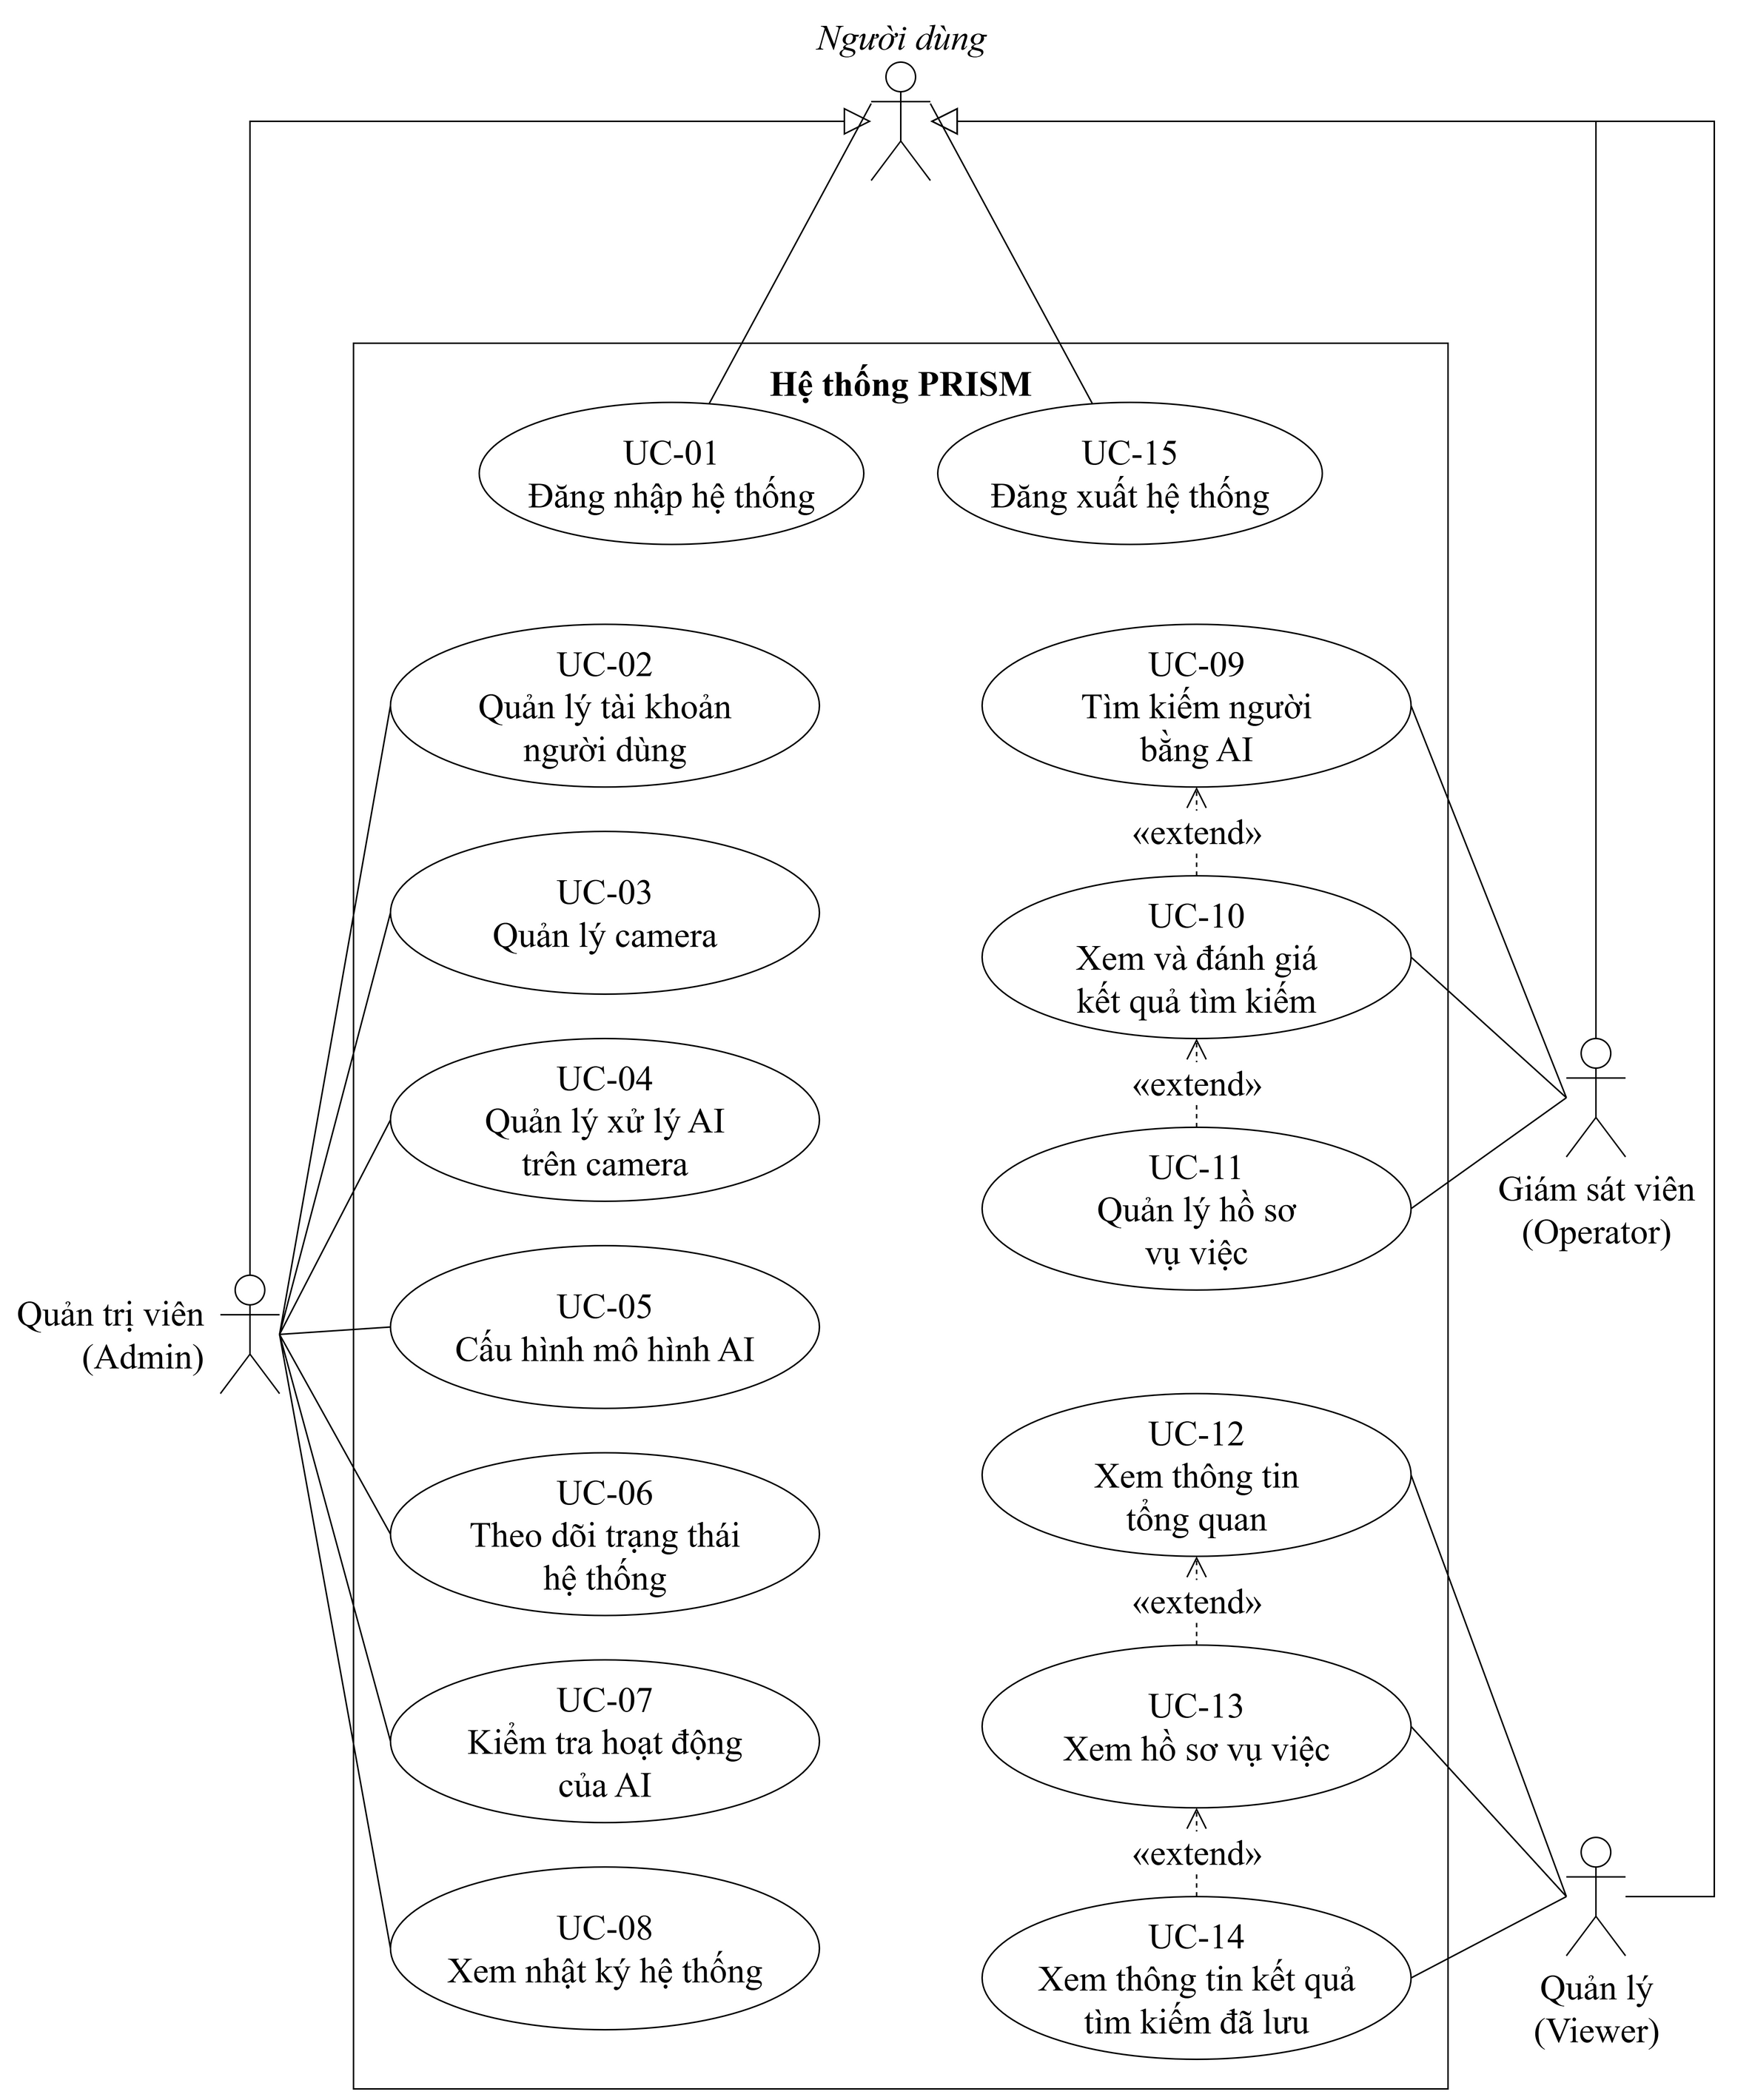
\includegraphics[width=\textwidth]{H1-use-case.png}
\caption{Sơ đồ use case tổng thể của hệ thống}
\label{fig:usecase}
\end{figure}

Sơ đồ theo bốn lựa chọn sau:
\begin{itemize}
    \item \textbf{Tác nhân trừu tượng \emph{Người dùng}.} Đăng nhập (UC-01) và đăng xuất (UC-15) được nối với tác nhân trừu tượng \emph{Người dùng}, mà ba tác nhân cụ thể tổng quát hóa về.
    \item \textbf{Phân chia theo vai trò.} Quản trị viên có UC-02 đến UC-08, Giám sát viên UC-09 đến UC-11, Quản lý UC-12 đến UC-14, không use case nào dùng chung.
    \item \textbf{Quan hệ mở rộng.} UC-10 mở rộng UC-09 và UC-11 mở rộng UC-10 (tìm kiếm, xem một kết quả, lưu vào vụ việc); tương tự, UC-13 mở rộng UC-12 và UC-14 mở rộng UC-13. Các use case mở rộng vẫn nối với tác nhân, vì tác nhân có thể bắt đầu chúng độc lập, chẳng hạn mở danh sách vụ việc mà không tìm kiếm.
    \item \textbf{Đăng nhập là tiền điều kiện} của mọi use case khác, không phải một bước bên trong, nên không vẽ quan hệ «include» tới UC-01.
\end{itemize}

Các chức năng tự động (Mục~\ref{sec:4.2.5}) không có use case riêng vì không do tác nhân nào kích hoạt; chúng chạy khi xử lý AI được bật trong UC-04.

\begin{table}[H]
\centering
\caption{Danh sách use case của hệ thống}
\label{tab:usecases}
\begin{tabularx}{\textwidth}{|>{\raggedright\arraybackslash}p{1.4cm}|>{\raggedright\arraybackslash}p{3.8cm}|>{\raggedright\arraybackslash}p{2.4cm}|L|}
\hline
\textbf{Mã} & \textbf{Tên use case} & \textbf{Tác nhân} & \textbf{Mục đích} \\
\hline
UC-01 & Đăng nhập hệ thống & Cả ba tác nhân & Xác thực và truy cập các chức năng theo vai trò \\
\hline
UC-02 & Quản lý tài khoản người dùng & Quản trị viên & Tạo, cập nhật, khóa, xóa tài khoản; gán vai trò và khu vực \\
\hline
UC-03 & Quản lý camera & Quản trị viên & Thêm, cập nhật camera, kiểm tra kết nối RTSP, loại khỏi và đưa lại vận hành \\
\hline
UC-04 & Quản lý xử lý AI trên camera & Quản trị viên & Bật, tắt xử lý AI cho từng camera; xử lý tệp video dự phòng \\
\hline
UC-05 & Cấu hình mô hình AI & Quản trị viên & Chọn Detector và Tracker áp dụng cho toàn hệ thống \\
\hline
UC-06 & Theo dõi trạng thái hệ thống & Quản trị viên & Theo dõi trạng thái camera, luồng RTSP và xử lý AI \\
\hline
UC-07 & Kiểm tra hoạt động của AI & Quản trị viên & Kiểm tra nhóm xử lý camera và nhóm tìm kiếm \\
\hline
UC-08 & Xem nhật ký hệ thống & Quản trị viên & Tra cứu nhật ký thao tác và sự kiện kỹ thuật \\
\hline
UC-09 & Tìm kiếm người bằng AI & Giám sát viên & Tìm người bằng ảnh, câu mô tả hoặc thuộc tính trong khu vực được gán \\
\hline
UC-10 & Xem và đánh giá kết quả tìm kiếm & Giám sát viên & Xem chi tiết, đối chiếu và đánh giá từng kết quả \\
\hline
UC-11 & Quản lý hồ sơ vụ việc & Giám sát viên & Tạo vụ việc, lưu kết quả, cập nhật, đánh dấu hoàn thành, mở lại \\
\hline
UC-12 & Xem thông tin tổng quan & Quản lý & Xem các chỉ số và vụ việc gần đây trên toàn hệ thống \\
\hline
UC-13 & Xem hồ sơ vụ việc & Quản lý & Xem mọi vụ việc ở chế độ chỉ đọc \\
\hline
UC-14 & Xem thông tin kết quả tìm kiếm đã lưu & Quản lý & Xem chi tiết kết quả đã lưu trong vụ việc \\
\hline
UC-15 & Đăng xuất hệ thống & Cả ba tác nhân & Kết thúc phiên làm việc \\
\hline
\end{tabularx}
\end{table}

% !TEX root = ../../main.tex
% C4.5 — Đặc tả use case. RÚT GỌN 2026-09-29 (SV duyệt): 8 use case của luồng nghiệp vụ chính UC-01, 03, 04, 05, 09, 10, 11, 13;
% viết gọn từ files/usecase_detail.md (gộp bước, bỏ ngoại lệ chung "lỗi hệ thống" và luồng thay thế trùng luồng chính), không thêm hành vi mới.
% Sinh bằng scratchpad uc_condensed.py (bản cũ đủ 15 UC ở report/archive/2026-09-29-truoc-khi-rut-gon/). Không dùng lại tools/usecase_to_tex.py cho tệp này.
\section{Đặc tả use case}
\label{sec:4.5}

Mục này đặc tả tám use case tạo thành luồng nghiệp vụ chính của hệ thống: người dùng đăng nhập (UC-01); Quản trị viên thêm camera (UC-03), đưa camera vào phân tích (UC-04) và chọn mô hình AI (UC-05); Giám sát viên tìm kiếm người (UC-09), đánh giá kết quả (UC-10) và lưu kết quả vào vụ việc (UC-11); Quản lý xem các hồ sơ vụ việc (UC-13). Mỗi đặc tả gồm tác nhân, mục đích, tiền điều kiện, hậu điều kiện, luồng chính, các ngoại lệ (ký hiệu E) và các luồng thay thế (ký hiệu A). Hành vi của các use case còn lại đã được nêu trong các yêu cầu chức năng ở Mục~\ref{sec:4.2}; phạm vi dữ liệu của từng vai trò được tổng hợp trong ma trận phân quyền ở Mục~\ref{sec:4.6}.

\begin{longtable}{|>{\raggedright\arraybackslash}p{2.9cm}|p{12.3cm}|}
\caption{Đặc tả use case UC-01: Đăng nhập hệ thống}\label{tab:uc01}\\
\hline
\textbf{Tác nhân} & Quản trị viên, Giám sát viên, Quản lý \\ \hline
\textbf{Mục đích} & Xác thực tài khoản để truy cập các chức năng và dữ liệu phù hợp với vai trò của người dùng. \\ \hline
\textbf{Tiền điều kiện} & Người dùng đã có tài khoản đang ở trạng thái hoạt động. \\ \hline
\textbf{Hậu điều kiện} & Hệ thống tạo phiên đăng nhập và đưa người dùng tới trang chủ của vai trò. \\ \hline
\endfirsthead
\multicolumn{2}{l}{\textit{(tiếp theo Bảng~\ref{tab:uc01})}}\\
\hline
\endhead
\textbf{Luồng chính} & \hangindent=1.6em\hangafter=1\noindent\makebox[1.6em][l]{1.}Người dùng mở trang đăng nhập, nhập tên đăng nhập và mật khẩu. \\ 
 & \hangindent=1.6em\hangafter=1\noindent\makebox[1.6em][l]{2.}Hệ thống kiểm tra thông tin đăng nhập và trạng thái của tài khoản. \\ 
 & \hangindent=1.6em\hangafter=1\noindent\makebox[1.6em][l]{3.}Hệ thống tạo phiên đăng nhập và xác định vai trò của tài khoản. \\ 
 & \hangindent=1.6em\hangafter=1\noindent\makebox[1.6em][l]{4.}Hệ thống đưa người dùng tới trang chủ của vai trò; người dùng chỉ thấy các chức năng thuộc vai trò đó. \\ \hline
\textbf{Ngoại lệ} & \textbf{E1 - Sai thông tin đăng nhập:} Hệ thống thông báo đăng nhập không thành công, với cùng một thông báo cho trường hợp sai tên đăng nhập và sai mật khẩu; lần thất bại được ghi vào nhật ký hệ thống. \\ \cline{2-2}
 & \textbf{E2 - Tài khoản bị khóa hoặc ngừng hoạt động:} Hệ thống từ chối đăng nhập. \\ \cline{2-2}
 & \textbf{E3 - Thử đăng nhập quá nhiều lần:} Nếu có quá nhiều lần đăng nhập trong thời gian ngắn, hệ thống tạm từ chối và cho biết thời gian cần chờ trước khi thử lại. \\ \hline
\textbf{Luồng thay thế} & Không có. \\ \hline
\end{longtable}

\begin{longtable}{|>{\raggedright\arraybackslash}p{2.9cm}|p{12.3cm}|}
\caption{Đặc tả use case UC-03: Quản lý camera}\label{tab:uc03}\\
\hline
\textbf{Tác nhân} & Quản trị viên \\ \hline
\textbf{Mục đích} & Quản lý các camera của hệ thống: thêm, cập nhật, kiểm tra kết nối RTSP, loại camera khỏi vận hành và đưa camera vận hành trở lại. \\ \hline
\textbf{Tiền điều kiện} & Quản trị viên đã đăng nhập; danh mục khu vực giám sát đã được khai báo. \\ \hline
\textbf{Hậu điều kiện} & Thông tin và trạng thái vận hành của camera được cập nhật; kết quả kiểm tra kết nối RTSP được ghi nhận. \\ \hline
\endfirsthead
\multicolumn{2}{l}{\textit{(tiếp theo Bảng~\ref{tab:uc03})}}\\
\hline
\endhead
\textbf{Luồng chính} & \hangindent=1.6em\hangafter=1\noindent\makebox[1.6em][l]{1.}Quản trị viên mở chức năng quản lý camera; hệ thống hiển thị danh sách camera cùng khu vực, trạng thái vận hành, trạng thái kết nối RTSP và xử lý AI. \\ 
 & \hangindent=1.6em\hangafter=1\noindent\makebox[1.6em][l]{2.}Quản trị viên chọn thêm camera và nhập mã, tên, khu vực và địa chỉ RTSP, có thể kèm tên đăng nhập và mật khẩu của camera; địa chỉ RTSP không bắt buộc với camera chỉ được xử lý bằng tệp video. \\ 
 & \hangindent=1.6em\hangafter=1\noindent\makebox[1.6em][l]{3.}Hệ thống kiểm tra dữ liệu, tách thông tin xác thực ra khỏi địa chỉ và lưu ở dạng mã hóa, rồi lưu camera ở trạng thái kết nối \emph{Chưa xác minh}. \\ 
 & \hangindent=1.6em\hangafter=1\noindent\makebox[1.6em][l]{4.}Hệ thống thử kết nối tới luồng RTSP và cập nhật trạng thái kết nối của camera. \\ \hline
\textbf{Ngoại lệ} & \textbf{E1 - Dữ liệu không hợp lệ:} Nếu thiếu thông tin bắt buộc, địa chỉ không phải địa chỉ RTSP hợp lệ, hoặc mã camera đã tồn tại, hệ thống từ chối lưu. \\ \cline{2-2}
 & \textbf{E2 - Không kết nối được:} Camera vẫn được lưu với trạng thái \emph{Mất kết nối} kèm cảnh báo; Quản trị viên có thể sửa cấu hình và kiểm tra lại sau. \\ \cline{2-2}
 & \textbf{E3 - Địa chỉ ngoài dải mạng cho phép:} Nếu địa chỉ không phải địa chỉ IP thuộc dải mạng camera được khai báo khi triển khai, hệ thống từ chối kiểm tra kết nối và camera giữ trạng thái \emph{Chưa xác minh}. \\ \hline
\textbf{Luồng thay thế} & \textbf{A1 - Cập nhật camera:} Quản trị viên sửa tên hoặc địa chỉ RTSP; khu vực của camera không đổi được. Khi địa chỉ thay đổi, trạng thái kết nối trở về \emph{Chưa xác minh} và được kiểm tra lại. \\ \cline{2-2}
 & \textbf{A2 - Kiểm tra lại kết nối:} Quản trị viên yêu cầu kiểm tra kết nối của một camera; hệ thống thử kết nối và cập nhật trạng thái. \\ \cline{2-2}
 & \textbf{A3 - Loại khỏi vận hành:} Camera chuyển sang ngừng vận hành, xử lý AI bị tắt và công việc đang chạy của camera bị hủy; dữ liệu đã tạo được giữ nguyên nhưng tạm thời không được tìm kiếm. \\ \cline{2-2}
 & \textbf{A4 - Đưa vận hành trở lại:} Camera vận hành trở lại với xử lý AI ở trạng thái tắt; dữ liệu cũ được tìm kiếm lại bình thường. \\ \hline
\end{longtable}

\begin{longtable}{|>{\raggedright\arraybackslash}p{2.9cm}|p{12.3cm}|}
\caption{Đặc tả use case UC-04: Quản lý xử lý AI trên camera}\label{tab:uc04}\\
\hline
\textbf{Tác nhân} & Quản trị viên \\ \hline
\textbf{Mục đích} & Quyết định camera nào được đưa vào quá trình phân tích AI bằng cách bật hoặc tắt xử lý AI cho từng camera, và xử lý tệp video ghi sẵn cho một camera khi cần. \\ \hline
\textbf{Tiền điều kiện} & Quản trị viên đã đăng nhập; camera đã được thêm vào hệ thống và đang vận hành. \\ \hline
\textbf{Hậu điều kiện} & Trạng thái xử lý AI của camera được cập nhật; hệ thống bắt đầu hoặc ngừng đưa camera vào quá trình phân tích. \\ \hline
\endfirsthead
\multicolumn{2}{l}{\textit{(tiếp theo Bảng~\ref{tab:uc04})}}\\
\hline
\endhead
\textbf{Luồng chính} & \hangindent=1.6em\hangafter=1\noindent\makebox[1.6em][l]{1.}Quản trị viên mở chức năng quản lý xử lý AI; hệ thống hiển thị danh sách camera cùng trạng thái xử lý AI và cấu hình mô hình đang áp dụng. \\ 
 & \hangindent=1.6em\hangafter=1\noindent\makebox[1.6em][l]{2.}Quản trị viên bật hoặc tắt xử lý AI cho một camera và xác nhận. \\ 
 & \hangindent=1.6em\hangafter=1\noindent\makebox[1.6em][l]{3.}Hệ thống kiểm tra trạng thái của camera và cấu hình mô hình hiện hành. \\ 
 & \hangindent=1.6em\hangafter=1\noindent\makebox[1.6em][l]{4.}Hệ thống lưu trạng thái mới. Khi bật, camera được phân tích lần lượt cùng các camera khác đang bật xử lý AI. Khi tắt, công việc đang chạy của camera bị hủy và hệ thống ngừng tạo dữ liệu mới; dữ liệu đã có được giữ nguyên. \\ 
 & \hangindent=1.6em\hangafter=1\noindent\makebox[1.6em][l]{5.}Hệ thống thông báo kết quả cho Quản trị viên. \\ \hline
\textbf{Ngoại lệ} & \textbf{E1 - Camera mất kết nối:} Nếu camera có RTSP đang mất kết nối, hệ thống từ chối bật xử lý AI và thông báo. \\ \cline{2-2}
 & \textbf{E2 - Mô hình AI chưa sẵn sàng:} Nếu cấu hình mô hình hiện hành chưa đầy đủ hoặc không khả dụng, hệ thống từ chối bật xử lý AI. \\ \cline{2-2}
 & \textbf{E3 - Camera không còn vận hành:} Nếu camera đã bị loại khỏi vận hành, hệ thống không cho phép thay đổi trạng thái xử lý AI. \\ \cline{2-2}
 & \textbf{E4 - Tệp video không hợp lệ:} Nếu tệp tải lên sai định dạng hoặc vượt dung lượng cho phép, hệ thống từ chối và không tạo công việc. \\ \hline
\textbf{Luồng thay thế} & \textbf{A1 - Xử lý tệp video:} Quản trị viên chọn một camera, tải lên tệp video ghi sẵn, chọn thời điểm bắt đầu ghi và chế độ lấy mẫu. Hệ thống kiểm tra tệp, tạo công việc xử lý đi qua cùng quy trình phân tích như luồng RTSP và hiển thị tiến độ. Đây là cách duy nhất để xử lý camera không có RTSP. \\ \hline
\end{longtable}

\begin{longtable}{|>{\raggedright\arraybackslash}p{2.9cm}|p{12.3cm}|}
\caption{Đặc tả use case UC-05: Cấu hình mô hình AI}\label{tab:uc05}\\
\hline
\textbf{Tác nhân} & Quản trị viên \\ \hline
\textbf{Mục đích} & Chọn mô hình phát hiện người (Detector) và thuật toán theo vết (Tracker) áp dụng chung cho toàn hệ thống. Bộ mã hóa ảnh và văn bản là thành phần cố định, không thay đổi được từ giao diện. \\ \hline
\textbf{Tiền điều kiện} & Quản trị viên đã đăng nhập; hệ thống đã có danh sách Detector và Tracker được đăng ký sẵn. \\ \hline
\textbf{Hậu điều kiện} & Cặp Detector-Tracker được chọn trở thành cấu hình hiện hành; các công việc xử lý được tạo sau đó dùng cấu hình này. \\ \hline
\endfirsthead
\multicolumn{2}{l}{\textit{(tiếp theo Bảng~\ref{tab:uc05})}}\\
\hline
\endhead
\textbf{Luồng chính} & \hangindent=1.6em\hangafter=1\noindent\makebox[1.6em][l]{1.}Quản trị viên mở chức năng cấu hình mô hình AI; hệ thống hiển thị cặp Detector-Tracker đang dùng và danh sách mô hình đã đăng ký, trong đó mô hình không khả dụng được đánh dấu và không chọn được. \\ 
 & \hangindent=1.6em\hangafter=1\noindent\makebox[1.6em][l]{2.}Quản trị viên chọn Detector, Tracker hoặc cả hai, rồi xác nhận áp dụng. \\ 
 & \hangindent=1.6em\hangafter=1\noindent\makebox[1.6em][l]{3.}Hệ thống kiểm tra các mô hình đã sẵn sàng và cặp Detector-Tracker tương thích với nhau, rồi nạp thử cấu hình mới. \\ 
 & \hangindent=1.6em\hangafter=1\noindent\makebox[1.6em][l]{4.}Hệ thống lưu cấu hình mới thành cấu hình hiện hành và thông báo kết quả. \\ \hline
\textbf{Ngoại lệ} & \textbf{E1 - Mô hình không khả dụng:} Nếu mô hình được chọn thiếu hoặc không nạp được, hệ thống từ chối áp dụng và giữ nguyên cấu hình hợp lệ trước đó. \\ \cline{2-2}
 & \textbf{E2 - Detector và Tracker không tương thích:} Hệ thống từ chối áp dụng và yêu cầu Quản trị viên chọn cặp khác. \\ \hline
\textbf{Luồng thay thế} & Không có. \\ \hline
\end{longtable}

\begin{longtable}{|>{\raggedright\arraybackslash}p{2.9cm}|p{12.3cm}|}
\caption{Đặc tả use case UC-09: Tìm kiếm người bằng AI}\label{tab:uc09}\\
\hline
\textbf{Tác nhân} & Giám sát viên \\ \hline
\textbf{Mục đích} & Tìm một người trong dữ liệu camera đã được phân tích bằng ảnh, câu mô tả tiếng Anh hoặc thuộc tính ngoại hình, trong phạm vi khu vực giám sát được giao. \\ \hline
\textbf{Tiền điều kiện} & Giám sát viên đã đăng nhập; tài khoản được gán một khu vực giám sát đã có dữ liệu được phân tích. \\ \hline
\textbf{Hậu điều kiện} & Hệ thống hiển thị tối đa $k$ kết quả phù hợp nhất trong phạm vi hợp lệ, xếp theo điểm phù hợp giảm dần. \\ \hline
\endfirsthead
\multicolumn{2}{l}{\textit{(tiếp theo Bảng~\ref{tab:uc09})}}\\
\hline
\endhead
\textbf{Luồng chính} & \hangindent=1.6em\hangafter=1\noindent\makebox[1.6em][l]{1.}Giám sát viên chọn hình thức tìm kiếm và cung cấp ảnh chứa người cần tìm, câu mô tả tiếng Anh hoặc các thuộc tính. \\ 
 & \hangindent=1.6em\hangafter=1\noindent\makebox[1.6em][l]{2.}Giám sát viên có thể chọn thêm camera thuộc khu vực và khoảng thời gian, chọn số kết quả $k$ trong các giá trị 4, 8, 12, 16, rồi gửi yêu cầu. \\ 
 & \hangindent=1.6em\hangafter=1\noindent\makebox[1.6em][l]{3.}Hệ thống kiểm tra dữ liệu truy vấn và tự giới hạn phạm vi tìm kiếm trong các camera đang vận hành thuộc khu vực của tài khoản. \\ 
 & \hangindent=1.6em\hangafter=1\noindent\makebox[1.6em][l]{4.}Hệ thống mã hóa truy vấn, so khớp với dữ liệu đã lập chỉ mục và lấy $k$ kết quả có điểm phù hợp cao nhất. \\ 
 & \hangindent=1.6em\hangafter=1\noindent\makebox[1.6em][l]{5.}Hệ thống hiển thị ảnh người, camera, khu vực, thời điểm xuất hiện và điểm phù hợp của từng kết quả. \\ \hline
\textbf{Ngoại lệ} & \textbf{E1 - Truy vấn không hợp lệ:} Nếu ảnh sai định dạng, câu mô tả không phải tiếng Anh, thuộc tính không hợp lệ hoặc $k$ không thuộc các giá trị cho phép, hệ thống báo lỗi và yêu cầu nhập lại. \\ \cline{2-2}
 & \textbf{E2 - Không có dữ liệu trong phạm vi:} Hệ thống thông báo không có dữ liệu phù hợp và gợi ý mở rộng khoảng thời gian hoặc chọn thêm camera. \\ \cline{2-2}
 & \textbf{E3 - Thành phần tìm kiếm không khả dụng:} Nếu bộ mã hóa hoặc kho vector không hoạt động, hệ thống báo tìm kiếm thất bại thay vì trả về danh sách rỗng. \\ \cline{2-2}
 & \textbf{E4 - Yêu cầu ngoài phạm vi:} Nếu yêu cầu gửi trực tiếp chứa camera không thuộc khu vực của tài khoản, máy chủ từ chối. \\ \hline
\textbf{Luồng thay thế} & \textbf{A1 - Tìm tiếp bằng một kết quả:} Giám sát viên kéo ảnh của một kết quả vào ô tìm kiếm bằng ảnh để tìm tiếp chính người đó. \\ \hline
\end{longtable}

\begin{longtable}{|>{\raggedright\arraybackslash}p{2.9cm}|p{12.3cm}|}
\caption{Đặc tả use case UC-10: Xem và đánh giá kết quả tìm kiếm}\label{tab:uc10}\\
\hline
\textbf{Tác nhân} & Giám sát viên \\ \hline
\textbf{Mục đích} & Xem chi tiết và đánh giá từng kết quả để xác định kết quả nào đúng là người cần tìm. \\ \hline
\textbf{Tiền điều kiện} & Giám sát viên đã thực hiện UC-09 và hệ thống đã trả về ít nhất một kết quả. \\ \hline
\textbf{Hậu điều kiện} & Giám sát viên đã đánh giá các kết quả; dữ liệu gốc không thay đổi. \\ \hline
\endfirsthead
\multicolumn{2}{l}{\textit{(tiếp theo Bảng~\ref{tab:uc10})}}\\
\hline
\endhead
\textbf{Luồng chính} & \hangindent=1.6em\hangafter=1\noindent\makebox[1.6em][l]{1.}Giám sát viên xem danh sách kết quả gồm ảnh người, camera, khu vực, thời điểm xuất hiện và điểm phù hợp. \\ 
 & \hangindent=1.6em\hangafter=1\noindent\makebox[1.6em][l]{2.}Giám sát viên chọn một kết quả; hệ thống hiển thị khung hình toàn cảnh có vẽ khung bao của người được tìm thấy, cùng thông tin chi tiết. \\ 
 & \hangindent=1.6em\hangafter=1\noindent\makebox[1.6em][l]{3.}Giám sát viên đối chiếu với người cần tìm và có thể tiếp tục xem các kết quả khác. \\ 
 & \hangindent=1.6em\hangafter=1\noindent\makebox[1.6em][l]{4.}Với kết quả muốn lưu, Giám sát viên chọn \textbf{Tạo vụ việc mới} hoặc \textbf{Thêm vào vụ việc đã có}; hệ thống chuyển sang UC-11. \\ \hline
\textbf{Ngoại lệ} & \textbf{E1 - Kết quả không còn khả dụng:} Nếu dữ liệu của kết quả đã bị loại bỏ, hệ thống thông báo kết quả không còn khả dụng. \\ \cline{2-2}
 & \textbf{E2 - Không hiển thị được ảnh:} Hệ thống vẫn hiển thị các thông tin còn lại và thông báo không hiển thị được ảnh người. \\ \hline
\textbf{Luồng thay thế} & \textbf{A1 - Sắp xếp kết quả:} Giám sát viên sắp xếp danh sách theo điểm phù hợp hoặc theo thời gian xuất hiện. \\ \cline{2-2}
 & \textbf{A2 - Lọc lại kết quả:} Giám sát viên lọc danh sách hiện tại theo camera hoặc khoảng thời gian mà không gửi truy vấn mới. \\ \hline
\end{longtable}

\begin{longtable}{|>{\raggedright\arraybackslash}p{2.9cm}|p{12.3cm}|}
\caption{Đặc tả use case UC-11: Quản lý hồ sơ vụ việc}\label{tab:uc11}\\
\hline
\textbf{Tác nhân} & Giám sát viên \\ \hline
\textbf{Mục đích} & Lưu các kết quả tìm kiếm liên quan đến một sự việc vào vụ việc do mình phụ trách, và theo dõi vụ việc cho tới khi hoàn thành. \\ \hline
\textbf{Tiền điều kiện} & Giám sát viên đã đăng nhập; kết quả cần lưu thuộc phạm vi tìm kiếm của Giám sát viên. \\ \hline
\textbf{Hậu điều kiện} & Vụ việc được tạo hoặc cập nhật, có đúng một Giám sát viên phụ trách, gồm tiêu đề, ghi chú, trạng thái và các kết quả đã lưu. \\ \hline
\endfirsthead
\multicolumn{2}{l}{\textit{(tiếp theo Bảng~\ref{tab:uc11})}}\\
\hline
\endhead
\textbf{Luồng chính} & \hangindent=1.6em\hangafter=1\noindent\makebox[1.6em][l]{1.}Từ một kết quả tìm kiếm, Giám sát viên chọn \textbf{Tạo vụ việc mới} hoặc \textbf{Thêm vào vụ việc đã có}. \\ 
 & \hangindent=1.6em\hangafter=1\noindent\makebox[1.6em][l]{2.}Với vụ việc mới, Giám sát viên nhập tiêu đề và ghi chú; hệ thống tự lấy tài khoản đang đăng nhập làm người phụ trách. Với vụ việc đã có, hệ thống chỉ hiển thị các vụ việc đang xử lý do chính Giám sát viên phụ trách để chọn. \\ 
 & \hangindent=1.6em\hangafter=1\noindent\makebox[1.6em][l]{3.}Hệ thống lưu kết quả thành một mục mới trong vụ việc, kể cả khi lần xuất hiện đó đã có trong vụ việc. \\ 
 & \hangindent=1.6em\hangafter=1\noindent\makebox[1.6em][l]{4.}Giám sát viên có thể sửa tiêu đề, ghi chú và loại bỏ kết quả khỏi vụ việc; dữ liệu gốc của lần xuất hiện không bị xóa. \\ 
 & \hangindent=1.6em\hangafter=1\noindent\makebox[1.6em][l]{5.}Khi xử lý xong, Giám sát viên đánh dấu vụ việc \textbf{Hoàn thành}; hệ thống ghi nhận thời điểm hoàn thành và khóa vụ việc. \\ \hline
\textbf{Ngoại lệ} & \textbf{E1 - Kết quả hoặc vụ việc không còn khả dụng:} Hệ thống thông báo, không lưu thay đổi và tải lại danh sách vụ việc. \\ \cline{2-2}
 & \textbf{E2 - Kết quả ngoài quyền truy cập:} Nếu yêu cầu gửi trực tiếp cố lưu một kết quả ngoài phạm vi của Giám sát viên, hệ thống từ chối. \\ \cline{2-2}
 & \textbf{E3 - Vụ việc đã hoàn thành:} Hệ thống từ chối thêm, loại kết quả hay sửa tiêu đề, ghi chú, và yêu cầu mở lại vụ việc trước. \\ \cline{2-2}
 & \textbf{E4 - Dữ liệu đã bị thay đổi ở nơi khác:} Hệ thống từ chối ghi đè và yêu cầu Giám sát viên tải lại vụ việc. \\ \hline
\textbf{Luồng thay thế} & \textbf{A1 - Đánh dấu hoàn thành ngay khi lưu:} Nếu Giám sát viên bật tùy chọn \textbf{Đánh dấu vụ việc đã hoàn thành} khi lưu, vụ việc được chuyển sang Hoàn thành ngay sau khi lưu; nếu bước này không thành công, kết quả vẫn được lưu và hệ thống thông báo để Giám sát viên đánh dấu lại. \\ \cline{2-2}
 & \textbf{A2 - Mở lại vụ việc:} Giám sát viên mở lại một vụ việc đã hoàn thành; vụ việc trở về \textbf{Đang xử lý} và có thể chỉnh sửa như bình thường. \\ \hline
\end{longtable}

\begin{longtable}{|>{\raggedright\arraybackslash}p{2.9cm}|p{12.3cm}|}
\caption{Đặc tả use case UC-13: Xem hồ sơ vụ việc}\label{tab:uc13}\\
\hline
\textbf{Tác nhân} & Quản lý \\ \hline
\textbf{Mục đích} & Xem mọi vụ việc do các Giám sát viên tạo cùng các kết quả đã lưu, ở chế độ chỉ đọc. \\ \hline
\textbf{Tiền điều kiện} & Quản lý đã đăng nhập. \\ \hline
\textbf{Hậu điều kiện} & Quản lý xem được nội dung của vụ việc; không có dữ liệu nào bị thay đổi. \\ \hline
\endfirsthead
\multicolumn{2}{l}{\textit{(tiếp theo Bảng~\ref{tab:uc13})}}\\
\hline
\endhead
\textbf{Luồng chính} & \hangindent=1.6em\hangafter=1\noindent\makebox[1.6em][l]{1.}Quản lý mở chức năng xem hồ sơ vụ việc; hệ thống hiển thị danh sách mọi vụ việc trong hệ thống. \\ 
 & \hangindent=1.6em\hangafter=1\noindent\makebox[1.6em][l]{2.}Quản lý có thể lọc theo trạng thái, khoảng thời gian tạo hoặc Giám sát viên phụ trách, rồi chọn một vụ việc. \\ 
 & \hangindent=1.6em\hangafter=1\noindent\makebox[1.6em][l]{3.}Hệ thống hiển thị tiêu đề, ghi chú, trạng thái, Giám sát viên phụ trách, thời gian tạo và các kết quả đã lưu, không kèm điểm phù hợp. \\ 
 & \hangindent=1.6em\hangafter=1\noindent\makebox[1.6em][l]{4.}Quản lý có thể chọn một kết quả để xem chi tiết; hệ thống chuyển sang UC-14 (Xem thông tin kết quả tìm kiếm đã lưu). \\ \hline
\textbf{Ngoại lệ} & \textbf{E1 - Chưa có vụ việc:} Hệ thống hiển thị trạng thái không có dữ liệu. \\ \cline{2-2}
 & \textbf{E2 - Vụ việc không truy xuất được:} Hệ thống thông báo không thể hiển thị hồ sơ và cho phép thử lại. \\ \cline{2-2}
 & \textbf{E3 - Một số kết quả không còn khả dụng:} Hệ thống vẫn hiển thị vụ việc cùng các dữ liệu còn lại và đánh dấu những kết quả không truy xuất được. \\ \hline
\textbf{Luồng thay thế} & \textbf{A1 - Mở từ màn hình tổng quan:} Quản lý chọn một vụ việc trong danh sách vụ việc gần đây của UC-12; hệ thống mở trực tiếp chi tiết vụ việc đó. \\ \hline
\end{longtable}

% !TEX root = ../../main.tex
% C4.6 — Ma trận phân quyền
% Nguồn: architect.md mục 4 (khu vực, camera, quyền) và mục 7 (ma trận quyền tóm tắt); usecase_detail.md ghi chú UC-03, UC-09, UC-11.
% "Không mặc định" của architect §7 viết là "Không" trong bảng, giải thích bằng câu ngay dưới bảng (khớp 4.1.1).
% Chương 8 (Mục 8.3) dùng bảng này làm căn cứ kiểm thử phân quyền.
\section{Ma trận phân quyền}
\label{sec:4.6}

Ngoài chức năng của từng tác nhân (Hình~\ref{fig:usecase}), các vai trò còn khác nhau ở \emph{phạm vi dữ liệu} được truy cập. Bảng~\ref{tab:permissions} nêu quyền của từng vai trò theo nhóm hành động, kèm các điều kiện này.

\begin{table}[H]
\centering
\caption{Ma trận phân quyền theo vai trò}
\label{tab:permissions}
\begin{tabularx}{\textwidth}{|>{\raggedright\arraybackslash}p{4.4cm}|L|L|L|}
\hline
\textbf{Nhóm hành động} & \textbf{Quản trị viên} & \textbf{Giám sát viên} & \textbf{Quản lý} \\
\hline
Đăng nhập, đăng xuất & Có & Có & Có \\
\hline
Quản lý tài khoản, gán khu vực cho Giám sát viên & Có & Không & Không \\
\hline
Quản lý camera, bật/tắt xử lý AI, tải video dự phòng, chọn Detector/Tracker & Có & Không & Không \\
\hline
Theo dõi trạng thái, kiểm tra hoạt động AI, xem nhật ký hệ thống & Có & Không & Không \\
\hline
Tìm kiếm người, xem ảnh và khung hình của kết quả tìm kiếm & Không & Chỉ trên các camera đang vận hành thuộc khu vực hiện tại & Không \\
\hline
Tạo vụ việc, thêm hoặc loại kết quả, sửa tiêu đề và ghi chú, đánh dấu hoàn thành hoặc mở lại & Không & Chỉ với vụ việc do mình phụ trách; kết quả thêm mới phải thuộc khu vực hiện tại & Không \\
\hline
Xem vụ việc và ảnh của kết quả đã lưu & Không & Vụ việc do mình phụ trách, kể cả sau khi được chuyển khu vực & Mọi vụ việc, chỉ đọc \\
\hline
Xem bảng tổng quan & Không & Không & Toàn hệ thống \\
\hline
\end{tabularx}
\end{table}

Ảnh của một lần xuất hiện được cấp theo một trong hai căn cứ: quyền tìm kiếm (camera đang vận hành trong khu vực hiện tại của Giám sát viên) hoặc quyền đối với vụ việc chứa nó. Căn cứ thứ hai cho Quản lý, và Giám sát viên đã đổi khu vực, xem được ảnh trong vụ việc dù không có quyền tìm kiếm trên camera đó. Mọi quyền đều được kiểm tra tại máy chủ (NFR-01).

Mục~\ref{sec:8.3} trình bày cách kiểm thử từng ô của ma trận này.


% !TEX root = ../../main.tex
% Chương 5 — xem mục C5 trong report/report_plan.md
\chapter{Thiết kế hệ thống}
\label{chapter:thietke}

\textit{Chương này trình bày thiết kế của hệ thống, gồm kiến trúc tổng thể, các luồng xử lý chính, cơ sở dữ liệu, giao diện lập trình, cơ chế bảo mật và giao diện người dùng.}

% !TEX root = ../../main.tex
% C5.1 — Thiết kế kiến trúc hệ thống (RÚT GỌN 2026-09-29: bỏ 5.1.2 "Hai luồng xử lý chính" vì trùng 5.2; bản cũ ở report/archive/)
% Nguồn: architect.md mục 3 (ranh giới thành phần, ba nơi lưu trữ), mục 1 (tuần tự, concurrency 1), mục 9, 13 (#4 RAM: chưa cần tách encoder).
% Khớp code: InProcessQueryEncoder trong app.py (encoder truy vấn chạy trong tiến trình API, trừ khi đặt PERSON_SEARCH_ENCODER_URL);
% hàng đợi = bảng processing_job trong PostgreSQL, worker nhận việc bằng lease + heartbeat (workers/durable.py);
% Vite proxy /api → Flask (frontend/vite.config). Hình H2: figures/H2-kien-truc.drawio (tools/h2_architecture_drawio.py).
\section{Thiết kế kiến trúc hệ thống}
\label{sec:5.1}

Hình~\ref{fig:architecture} trình bày kiến trúc tổng thể của hệ thống, tổ chức quanh hai giai đoạn đã nêu ở Mục~\ref{sec:3.1.6}: luồng \emph{lập chỉ mục} ở cột trái biến dữ liệu camera thành các lần xuất hiện có thể tìm kiếm, và luồng \emph{tìm kiếm} ở cột phải phục vụ thao tác của người dùng. Hai luồng gặp nhau ở tầng lưu trữ phía dưới.

\begin{figure}[!tbp]
\centering
% Rộng 18 cm, vượt đều mỗi bên lề 1 cm cho dễ đọc (lề trái còn 2 cm, lề phải còn 1 cm).
\makebox[\textwidth][c]{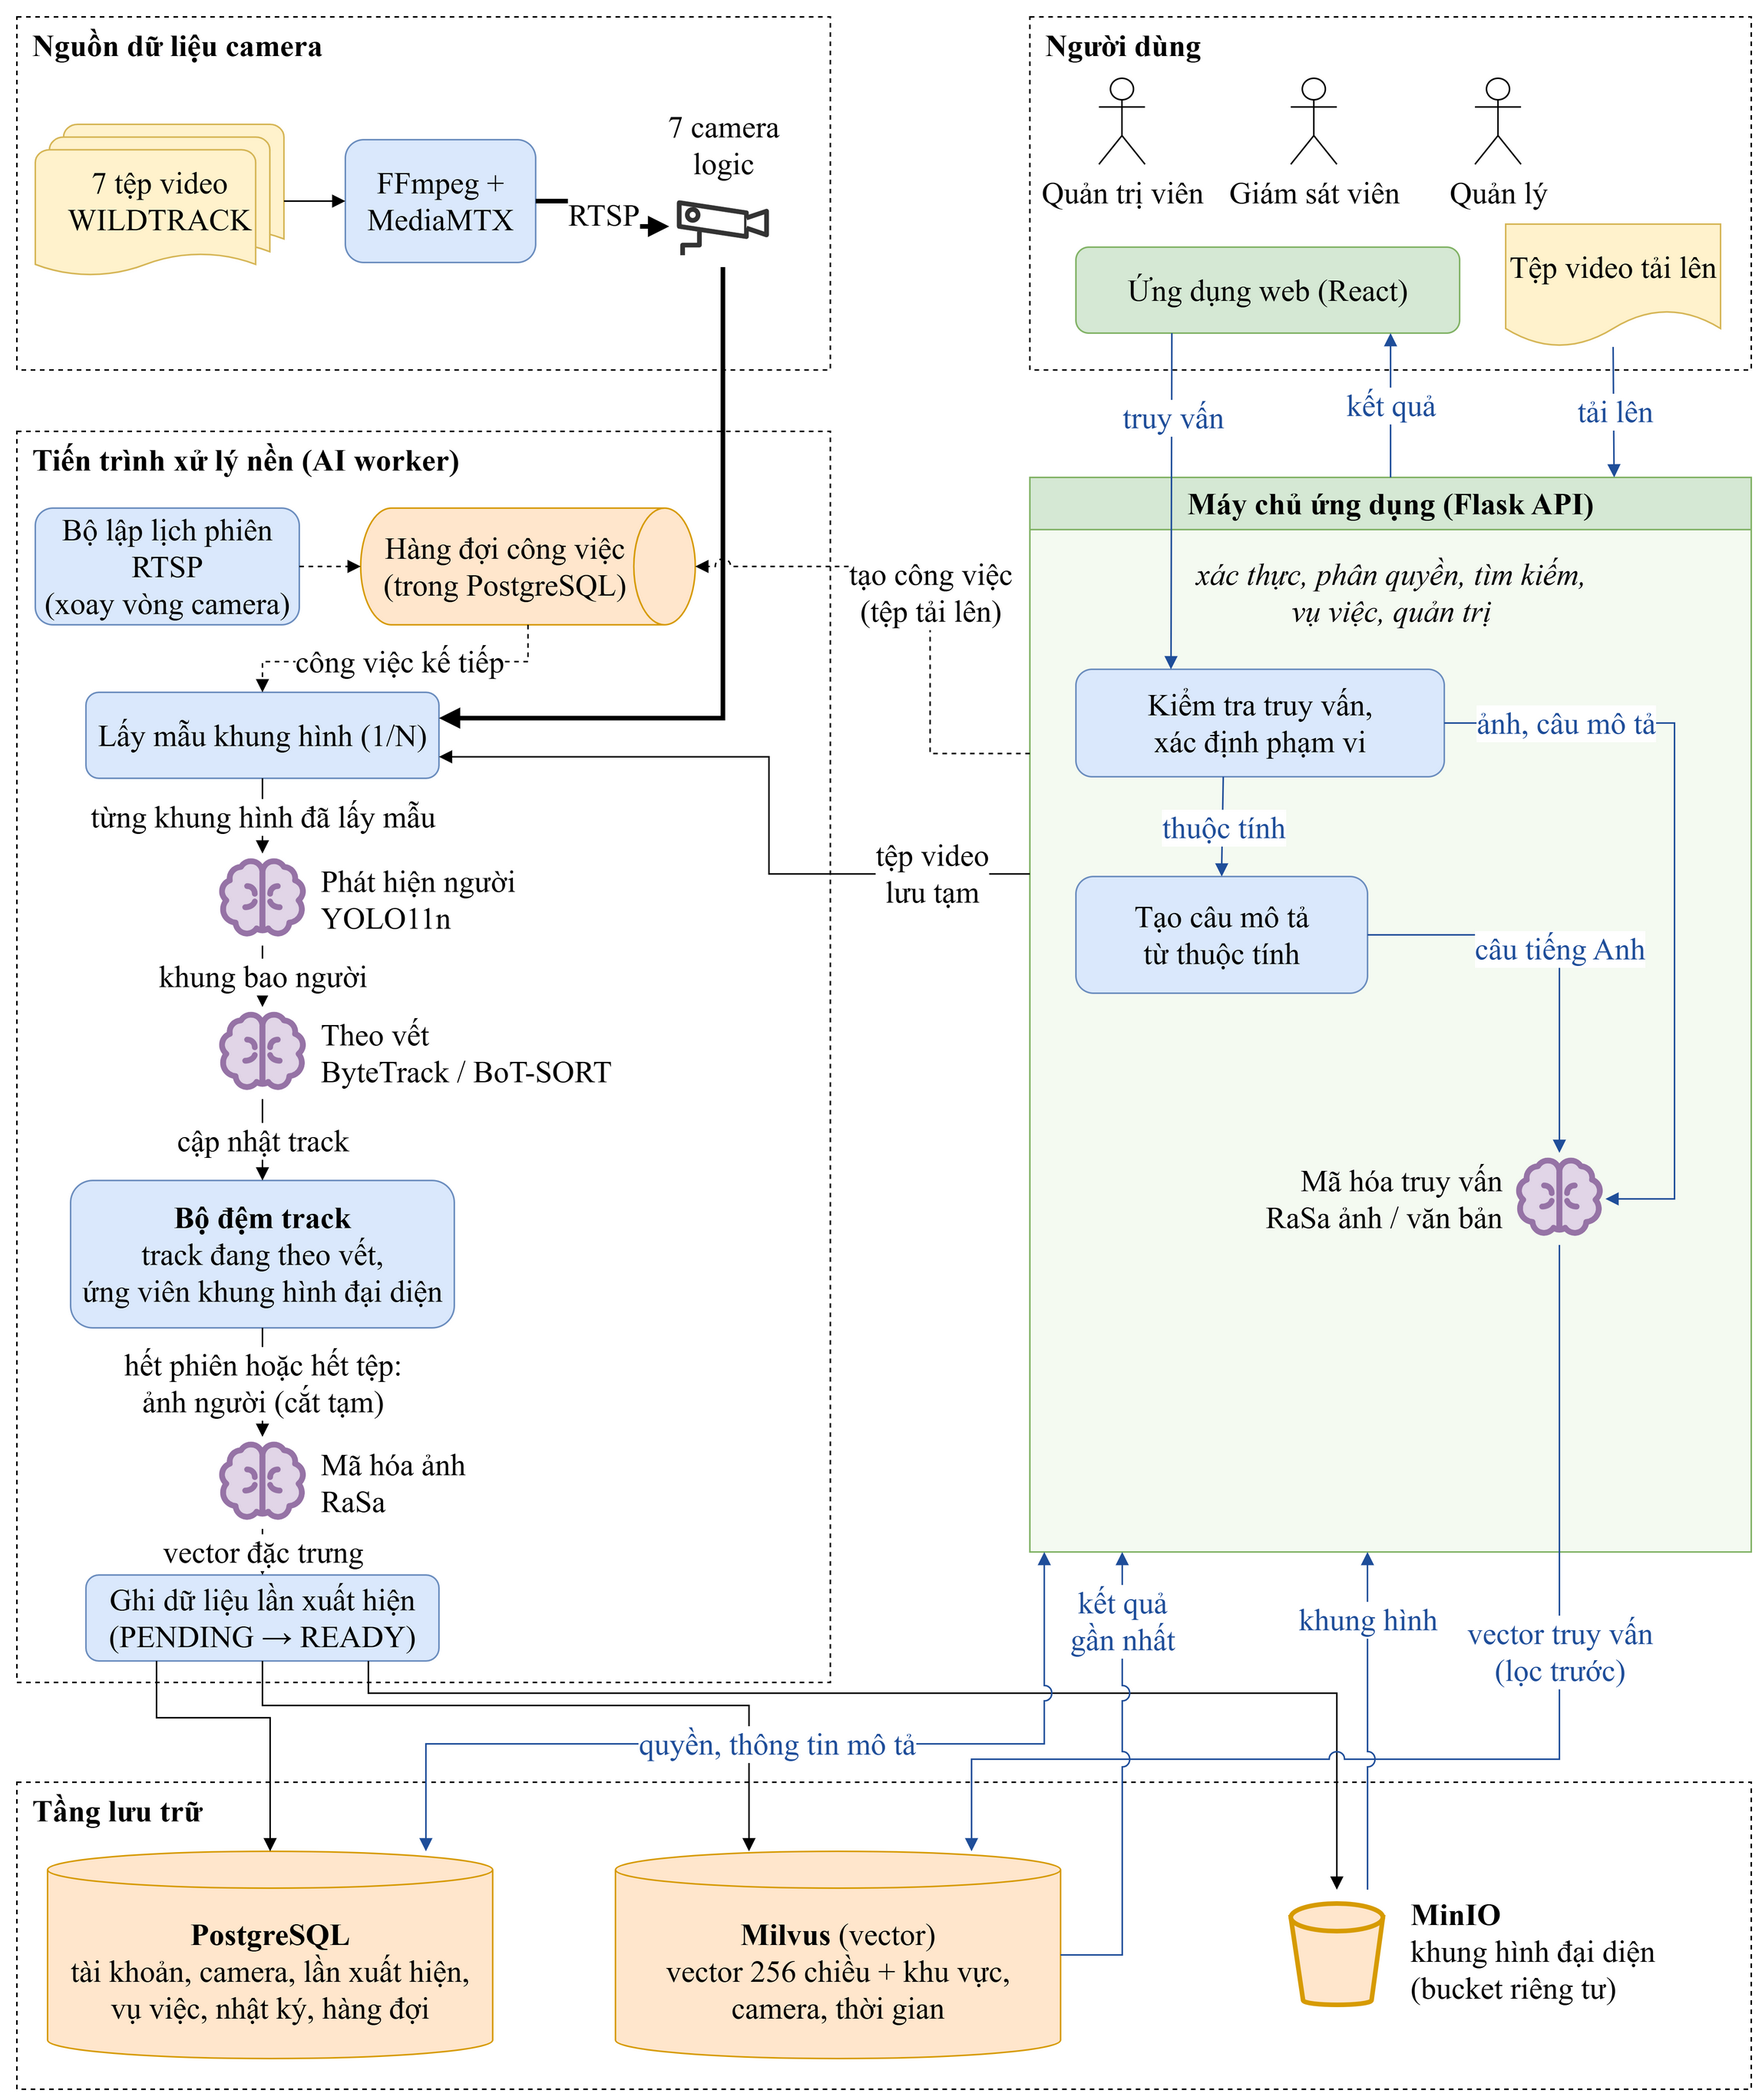
\includegraphics[width=18cm]{H2-kien-truc.png}}
\caption{Kiến trúc tổng thể của hệ thống}
\label{fig:architecture}
\end{figure}

\subsection{Các thành phần của hệ thống}
\label{sec:5.1.1}

\begin{itemize}
    \item \textbf{Nguồn dữ liệu camera.} Các tệp video của bộ dữ liệu thử nghiệm được FFmpeg phát liên tục lên máy chủ MediaMTX thành các luồng RTSP; mỗi luồng là một camera logic (Mục~\ref{sec:3.7.3}) và đối với hệ thống không khác camera IP thật.
    \item \textbf{Ứng dụng web.} Giao diện xây dựng bằng React, dùng chung cho cả ba vai trò; ứng dụng web chỉ giao tiếp với máy chủ ứng dụng, không truy cập trực tiếp kho dữ liệu nào.
    \item \textbf{Máy chủ ứng dụng.} Một tiến trình Flask cung cấp API cho toàn bộ chức năng, và nạp sẵn bộ mã hóa RaSa để mã hóa truy vấn tìm kiếm.
    \item \textbf{Tiến trình xử lý nền.} Một tiến trình Python riêng thực hiện toàn bộ phần xử lý AI: tự tạo các phiên xử lý RTSP xoay vòng giữa các camera, lần lượt nhận từng công việc trong hàng đợi và chạy quy trình phân tích.
    \item \textbf{Tầng lưu trữ.} PostgreSQL lưu dữ liệu nghiệp vụ và hàng đợi công việc; Milvus lưu vector đặc trưng kèm các trường dùng để lọc; MinIO lưu khung hình toàn cảnh đại diện của mỗi lần xuất hiện.
\end{itemize}

\subsection{Các nguyên tắc thiết kế}
\label{sec:5.1.3}

Nguyên tắc quan trọng nhất là tách xử lý AI khỏi máy chủ ứng dụng. Trên máy triển khai, việc phân tích video chậm hơn thời gian thực khoảng bảy lần, nên máy chủ ứng dụng không đọc luồng RTSP hay chạy quy trình phân tích mà chỉ tạo công việc. Tiến trình xử lý nền thực hiện các công việc này một cách độc lập. Người dùng vẫn tìm kiếm bình thường trong khi hệ thống đang lập chỉ mục, và lỗi khi phân tích không làm dừng máy chủ ứng dụng.

Hàng đợi công việc được đặt ngay trong PostgreSQL: mỗi công việc là một bản ghi, thay vì dùng thêm một hệ thống hàng đợi thông điệp riêng. Cách này giảm số thành phần phải triển khai trên máy cá nhân và giữ trạng thái công việc cùng chỗ với dữ liệu nghiệp vụ. Tiến trình xử lý nền thực hiện tuần tự một công việc tại một thời điểm, còn các phiên RTSP có thời lượng giới hạn được xoay vòng giữa các camera, để mọi camera đều lần lượt được phân tích mà không làm quá tải máy chỉ có CPU.

Về lưu trữ, mỗi kho giữ một loại dữ liệu và PostgreSQL là nơi quyết định. Ba phần của cùng một lần xuất hiện được liên kết bằng một mã chung, và mọi kết quả do Milvus trả về đều được đối chiếu lại với PostgreSQL trước khi hiển thị. Mọi truy cập dữ liệu, kể cả ảnh, đều đi qua máy chủ ứng dụng, để ma trận phân quyền ở Mục~\ref{sec:4.6} được áp dụng tại một điểm duy nhất.

Cuối cùng, hai luồng dùng chung bộ mã hóa và quy trình. Truy vấn được mã hóa bằng đúng trọng số RaSa đã dùng khi lập chỉ mục, để hai bên nằm trong cùng một không gian vector. Luồng RTSP và tệp video chỉ khác nhau ở bước đọc khung hình.

% !TEX root = ../../main.tex
% C5.2 — Thiết kế các luồng xử lý chính (RÚT GỌN 2026-09-29; bản cũ ở report/archive/)
% Khớp code: services/rtsp_scheduler.py (hàng đợi trống, camera ACTIVE + bật AI + có RTSP, lâu nhất chưa xử lý, bỏ qua camera lỗi 5 phút,
% 1.800 khung nguồn/phiên, profile throughput); services/jobs.py (claim, giữ chỗ 60 s, cancel, defer_retry); workers/durable.py (tối đa 3 lần);
% ai/selectors/representative.py + config (K=3, bộ đệm 256 MB, lọc cứng 24x48 px, phương sai độ nét >= 15, chạm < 2 cạnh, diện tích <= 4x,
% tỉ lệ <= 2,5x; điểm 0,30/0,25/0,20/0,15/0,10 trừ phạt biên 0,1/cạnh và che khuất <= 0,2; nới 5% khi cắt);
% services/track_ingestion.py (PENDING -> MinIO -> Milvus -> READY, thử lại lũy thừa tối đa 5 lần); services/searches.py (JPEG/PNG <= 10 MB,
% tạo câu từ thuộc tính); services/track_search.py; services/cases.py (_save_track: READY + camera ACTIVE thuộc khu vực hiện tại;
% snapshot tên camera/khu vực/thời điểm; version khi cập nhật; khóa khi CLOSED).
% ĐÃ SỬA 2026-09-29: workers/production.py chọn khung hình đại diện khi track kết thúc (selector._finalize), nhưng chỉ mã hóa + ghi
% sau khi hết nguồn/đủ số khung (selector.flush -> encode -> publish ở workers/durable.py); hủy/quá hạn -> không ghi. H3 và văn bản đã khớp.
\section{Thiết kế các luồng xử lý chính}
\label{sec:5.2}

\subsection{Luồng xử lý dữ liệu camera}
\label{sec:5.2.1}

Mọi hoạt động phân tích được tổ chức thành \emph{công việc xử lý} lưu trong hàng đợi, mỗi công việc gắn với một camera và một nguồn dữ liệu. Với \textbf{phiên RTSP tự động}, khi hàng đợi trống, bộ lập lịch trong tiến trình xử lý nền chọn một camera đang vận hành, đang bật xử lý AI và có địa chỉ RTSP, ưu tiên camera lâu nhất chưa được xử lý, rồi tạo một phiên giới hạn 1.800 khung hình nguồn, tương đương khoảng 30 giây video ở 60 khung hình mỗi giây; camera có phiên gần nhất thất bại được bỏ qua trong 5 phút để không chiếm lượt của các camera khác. Nhờ xoay vòng, các camera lần lượt được phân tích, nhưng giữa hai phiên của cùng một camera có những khoảng thời gian không được phân tích (Mục~\ref{sec:1.4}). Với \textbf{tệp video tải lên}, máy chủ ứng dụng kiểm tra tệp, lưu tạm và tạo công việc tương ứng.

\paragraph{Vòng đời công việc.} Hình~\ref{fig:job-state} mô tả các trạng thái của một công việc. Công việc mới ở trạng thái \emph{Chờ xử lý}. Khi tiến trình xử lý nền nhận việc, công việc chuyển sang \emph{Đang xử lý} kèm một thời hạn giữ chỗ 60 giây, được gia hạn định kỳ trong suốt quá trình xử lý; nếu tiến trình dừng đột ngột và thời hạn này trôi qua, công việc có thể được nhận lại. Với công việc xử lý tệp video, lỗi tạm thời được thử lại sau một khoảng chờ, tối đa ba lần; phiên RTSP gặp lỗi thì kết thúc ngay và camera được xử lý lại ở một phiên sau. Công việc kết thúc ở \emph{Hoàn thành}, \emph{Thất bại} khi gặp lỗi không phục hồi được hoặc hết số lần thử, hoặc \emph{Đã hủy} khi Quản trị viên yêu cầu hủy, khi camera bị loại khỏi vận hành hay bị tắt xử lý AI trong lúc công việc đang chờ hoặc đang chạy.

\begin{figure}[!htbp]
\centering
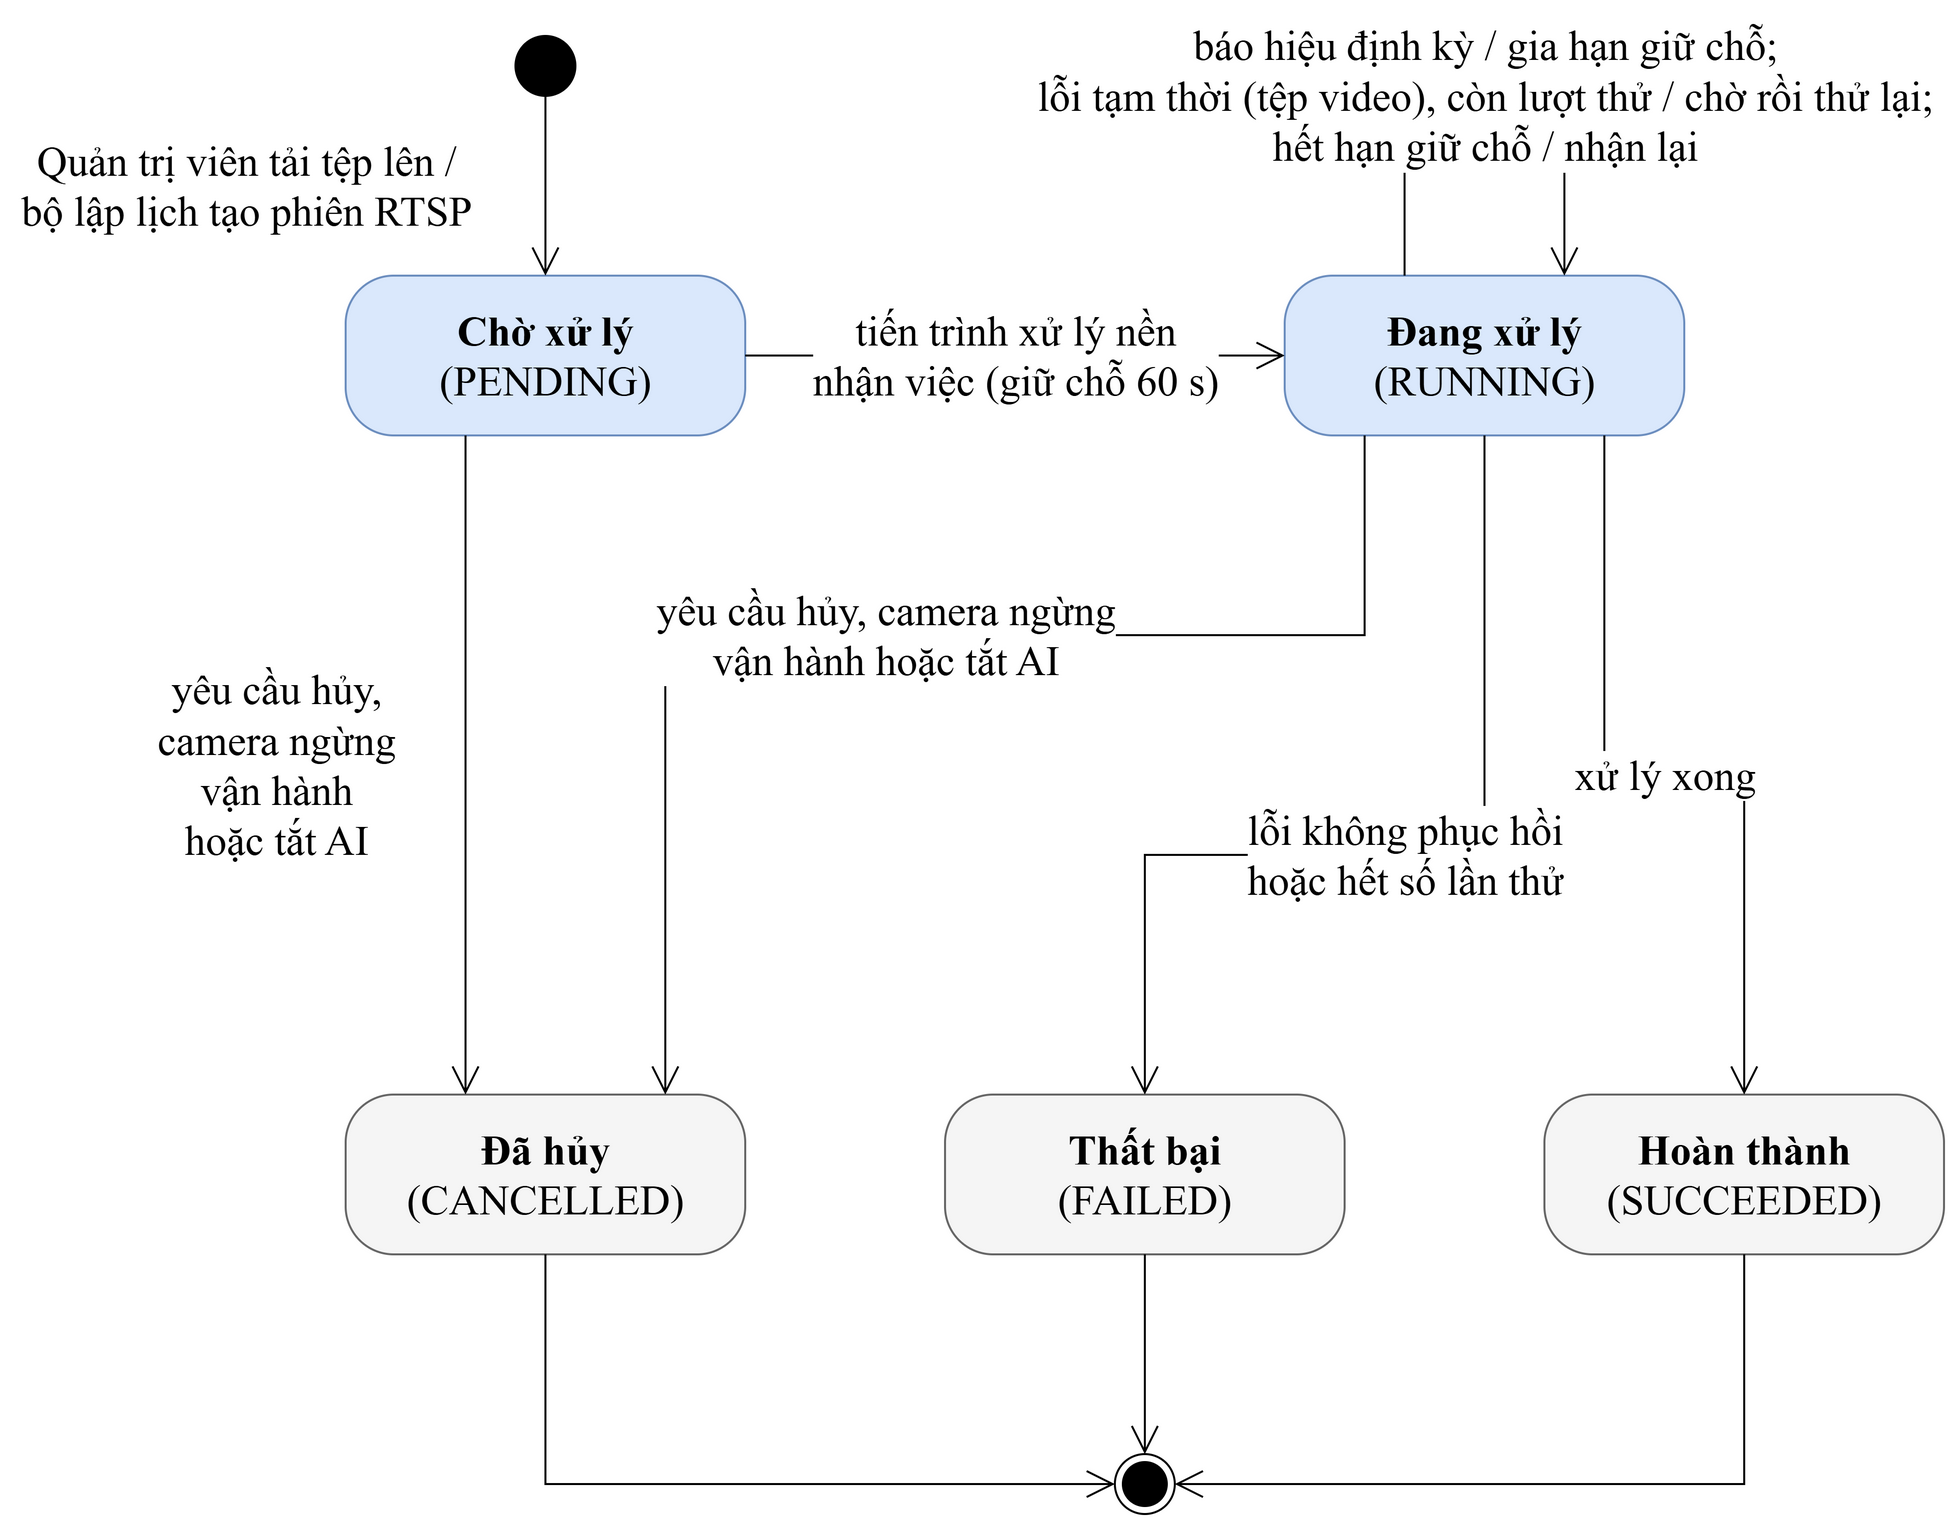
\includegraphics[width=\textwidth]{H7-trang-thai-cong-viec.png}
\caption{Sơ đồ trạng thái của công việc xử lý}
\label{fig:job-state}
\end{figure}

\paragraph{Các bước xử lý.} Hình~\ref{fig:pipeline-flow} trình bày lưu đồ xử lý một công việc, gồm hai giai đoạn. Trong \emph{vòng lặp theo khung hình}, mỗi khung hình được đọc kèm chỉ số và mốc thời gian (Mục~\ref{sec:3.7.4}), và chỉ một trong mỗi $N$ khung hình được đưa qua Detector và Tracker. Kết quả theo vết được cập nhật vào \emph{bộ đệm track}, nơi giữ các lần xuất hiện đang được theo vết cùng các ứng viên khung hình đại diện của chúng, rồi hệ thống chuyển sang khung hình tiếp theo. Khi lần xuất hiện kết thúc, khung hình đại diện được chọn và giữ lại trong bộ nhớ. Khi hết nguồn hoặc đủ số khung hình của phiên, các lần xuất hiện còn đang theo vết cũng được kết thúc, và công việc chuyển sang giai đoạn \emph{mã hóa và ghi}: với từng lần xuất hiện, vùng người trên khung hình đại diện được cắt tạm trong bộ nhớ, nới rộng mỗi phía 5\% kích thước khung bao, đưa qua bộ mã hóa ảnh để tạo vector đặc trưng, rồi được ghi vào ba kho theo thứ tự ở Mục~\ref{sec:5.3.4}. Như vậy, các lần xuất hiện của một công việc chỉ được tìm thấy sau khi công việc xử lý xong nguồn. Với luồng RTSP, nguồn của một công việc là một phiên 1.800 khung hình, nên dữ liệu của camera được ghi theo từng phiên: một người xuất hiện trước camera chỉ tìm kiếm được sau khi phiên chứa lần xuất hiện đó được xử lý xong. Nếu công việc bị hủy hoặc quá thời hạn trong lúc đọc và phân tích nguồn, không lần xuất hiện nào của nó được ghi. Mỗi lần xuất hiện được ghi kèm phiên bản cấu hình Detector-Tracker, phiên bản bộ mã hóa và khoảng lấy mẫu $N$ đã dùng.

\begin{figure}[!htbp]
\centering
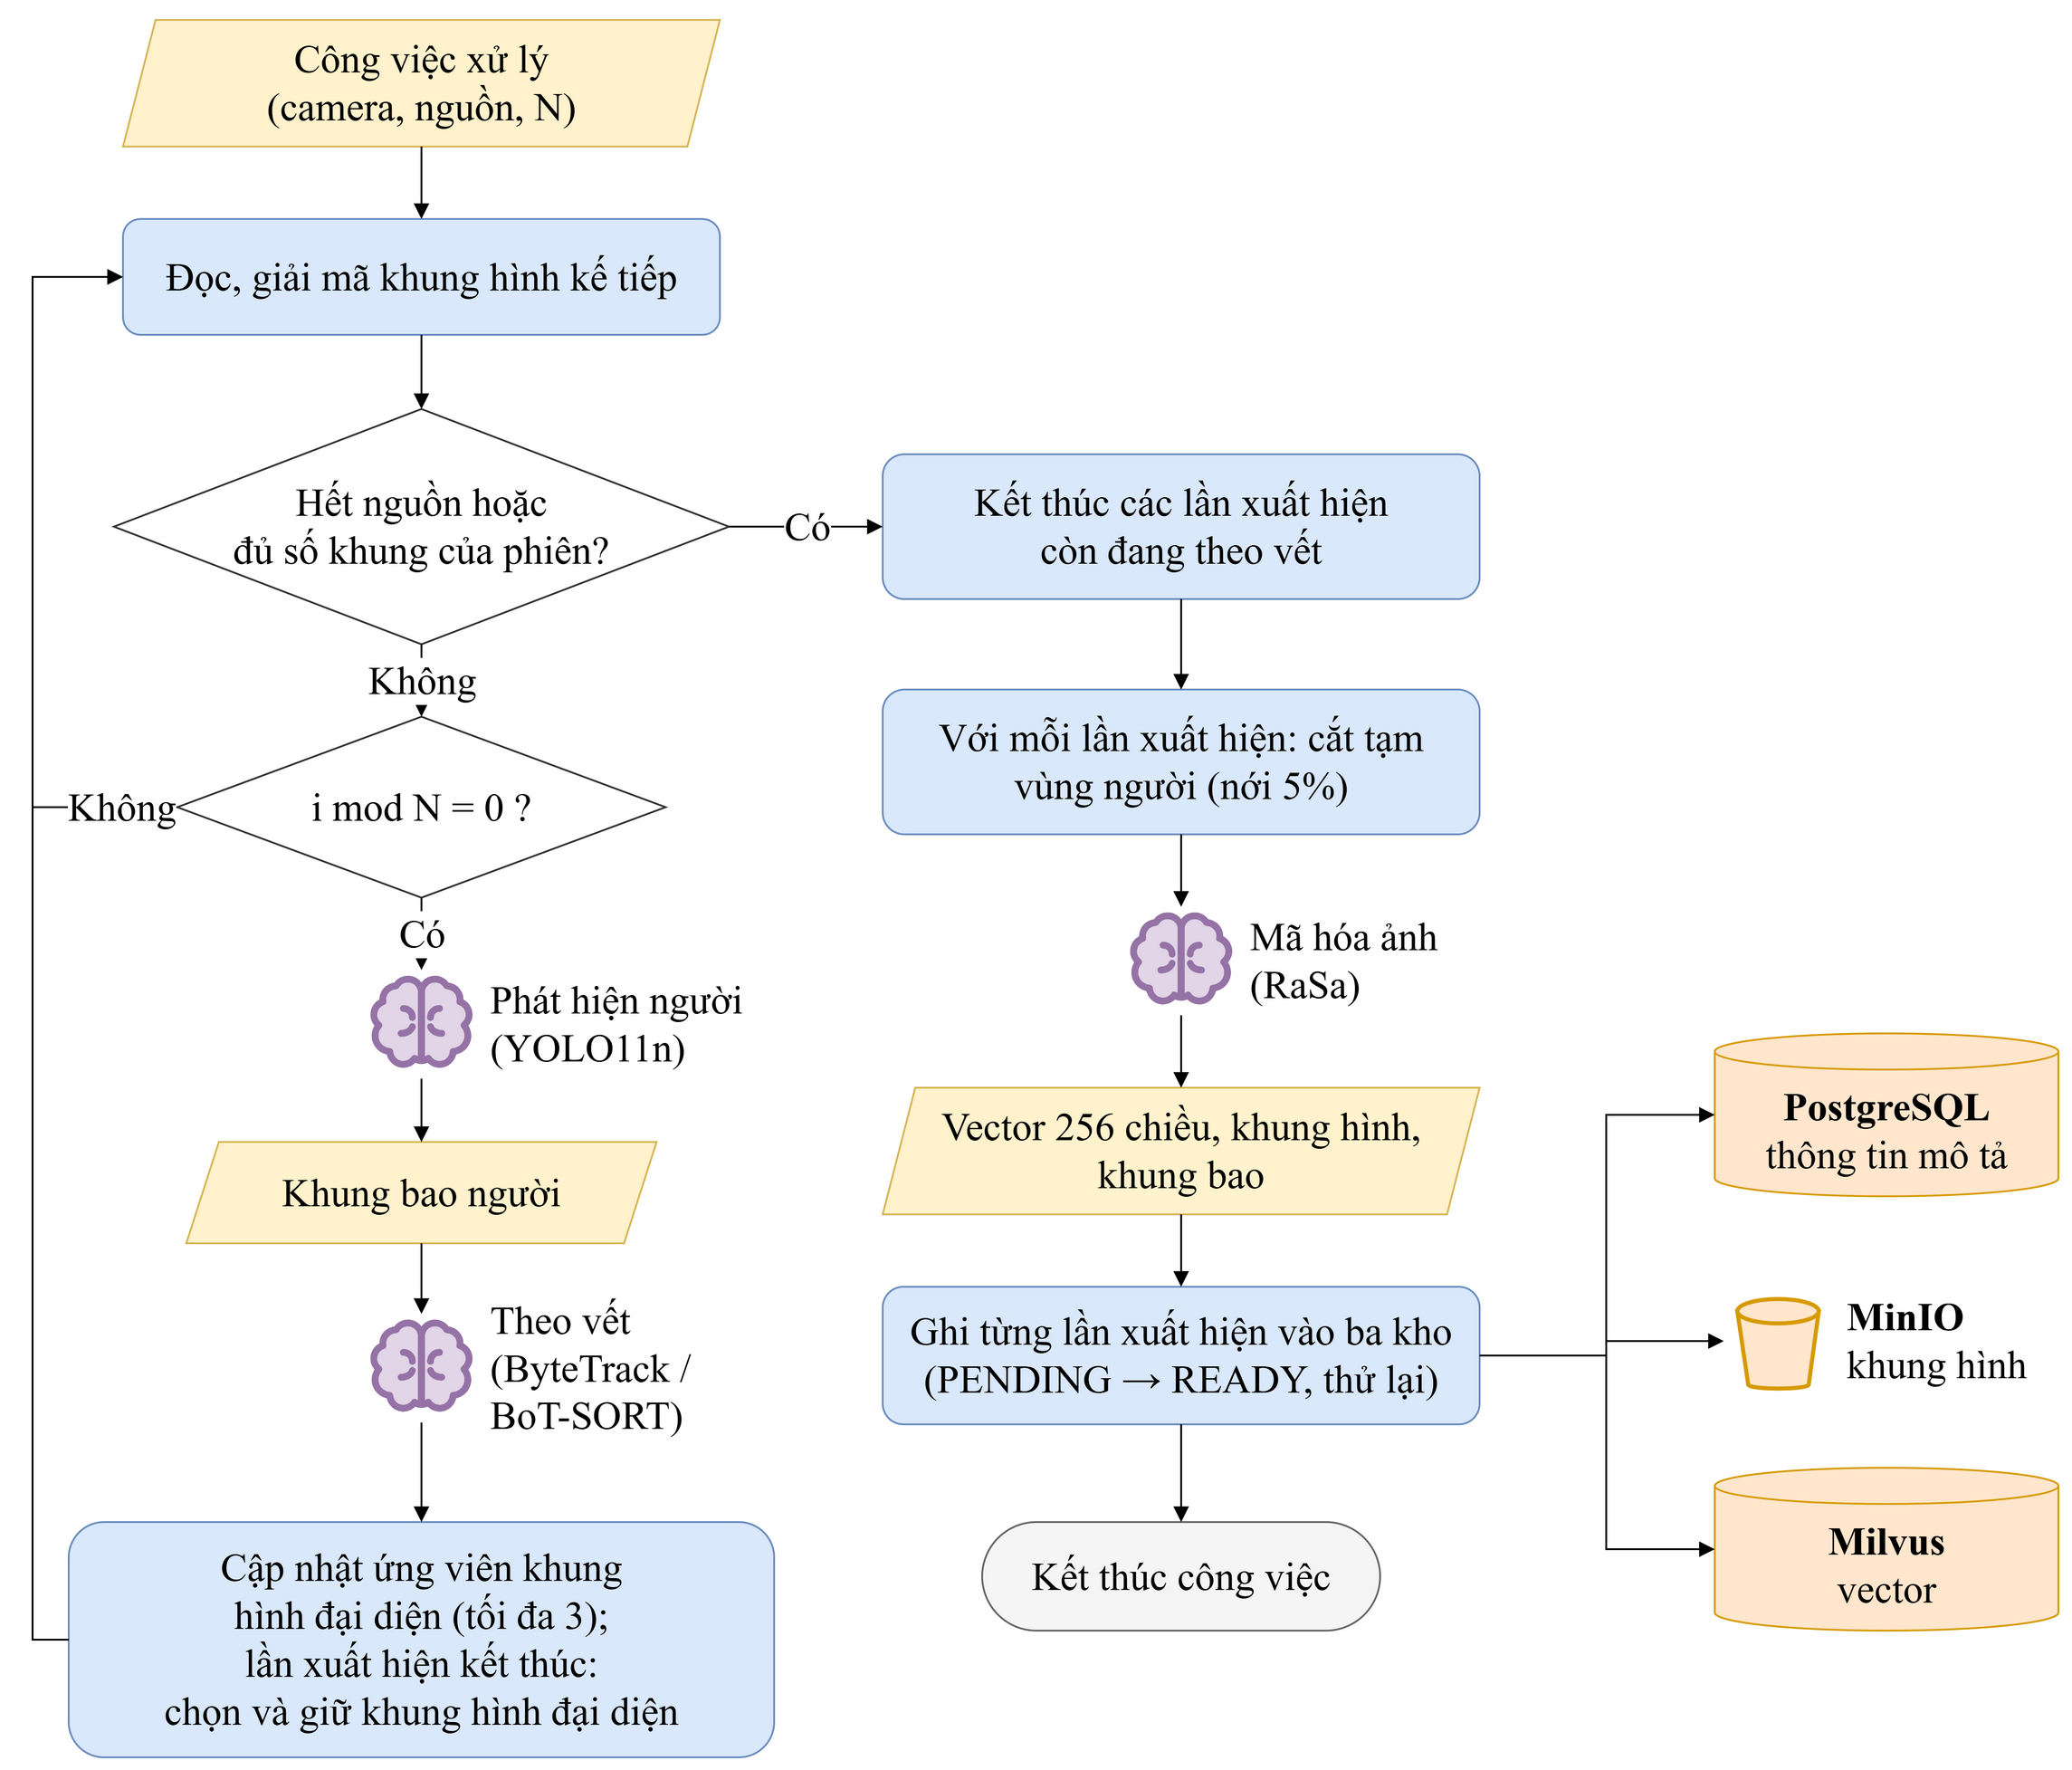
\includegraphics[width=\textwidth]{H3-luu-do-xu-ly-camera.png}
\caption{Lưu đồ xử lý một công việc}
\label{fig:pipeline-flow}
\end{figure}

\subsection{Chọn khung hình đại diện}
\label{sec:5.2.2}

Mỗi lần xuất hiện chỉ lưu \emph{một} khung hình toàn cảnh, dùng cho cả việc tạo vector lẫn hiển thị kết quả, nên khung hình này cần cho thấy người rõ nhất có thể. Bộ chọn khung hình đại diện hoạt động như sau:
\begin{itemize}
    \item \textbf{Giữ tối đa ba ứng viên} có điểm cao nhất cho mỗi lần xuất hiện đang diễn ra; tổng bộ nhớ cho các ứng viên của mọi lần xuất hiện được giới hạn ở 256~MB.
    \item \textbf{Lọc cứng.} Ứng viên chỉ đạt khi khung bao tối thiểu 24$\times$48 điểm ảnh, vùng người đủ nét, khung bao chạm ít hơn hai cạnh khung hình và không thay đổi hình dạng đột ngột so với lần quan sát trước (diện tích không đổi quá 4 lần, tỉ lệ rộng-cao không đổi quá 2,5 lần), vì thay đổi đột ngột thường là dấu hiệu nhầm người hoặc bị che khuất.
    \item \textbf{Điểm chất lượng} là tổng có trọng số của độ lớn người trong khung hình (0,30), độ nét (0,25), mức độ đầy đủ của thân người (0,20), độ ổn định so với lần quan sát trước (0,15) và vị trí gần giữa khoảng thời gian xuất hiện (0,10), trừ điểm phạt khi khung bao chạm cạnh khung hình hoặc chồng lấn người khác.
    \item \textbf{Chọn khi kết thúc.} Ứng viên có điểm cao nhất trong số các ứng viên đạt lọc cứng được chọn; nếu không có ứng viên nào đạt, ứng viên điểm cao nhất vẫn được chọn và lần xuất hiện được đánh dấu chất lượng thấp thay vì bị loại bỏ.
\end{itemize}
Các tiêu chí và trọng số được thiết kế theo kinh nghiệm, lưu thành tệp cấu hình, và cho kết quả xác định.

\subsection{Luồng tìm kiếm}
\label{sec:5.2.3}

Hình~\ref{fig:search-sequence} trình bày luồng tìm kiếm dưới dạng sơ đồ tuần tự.

\begin{figure}[!htbp]
\centering
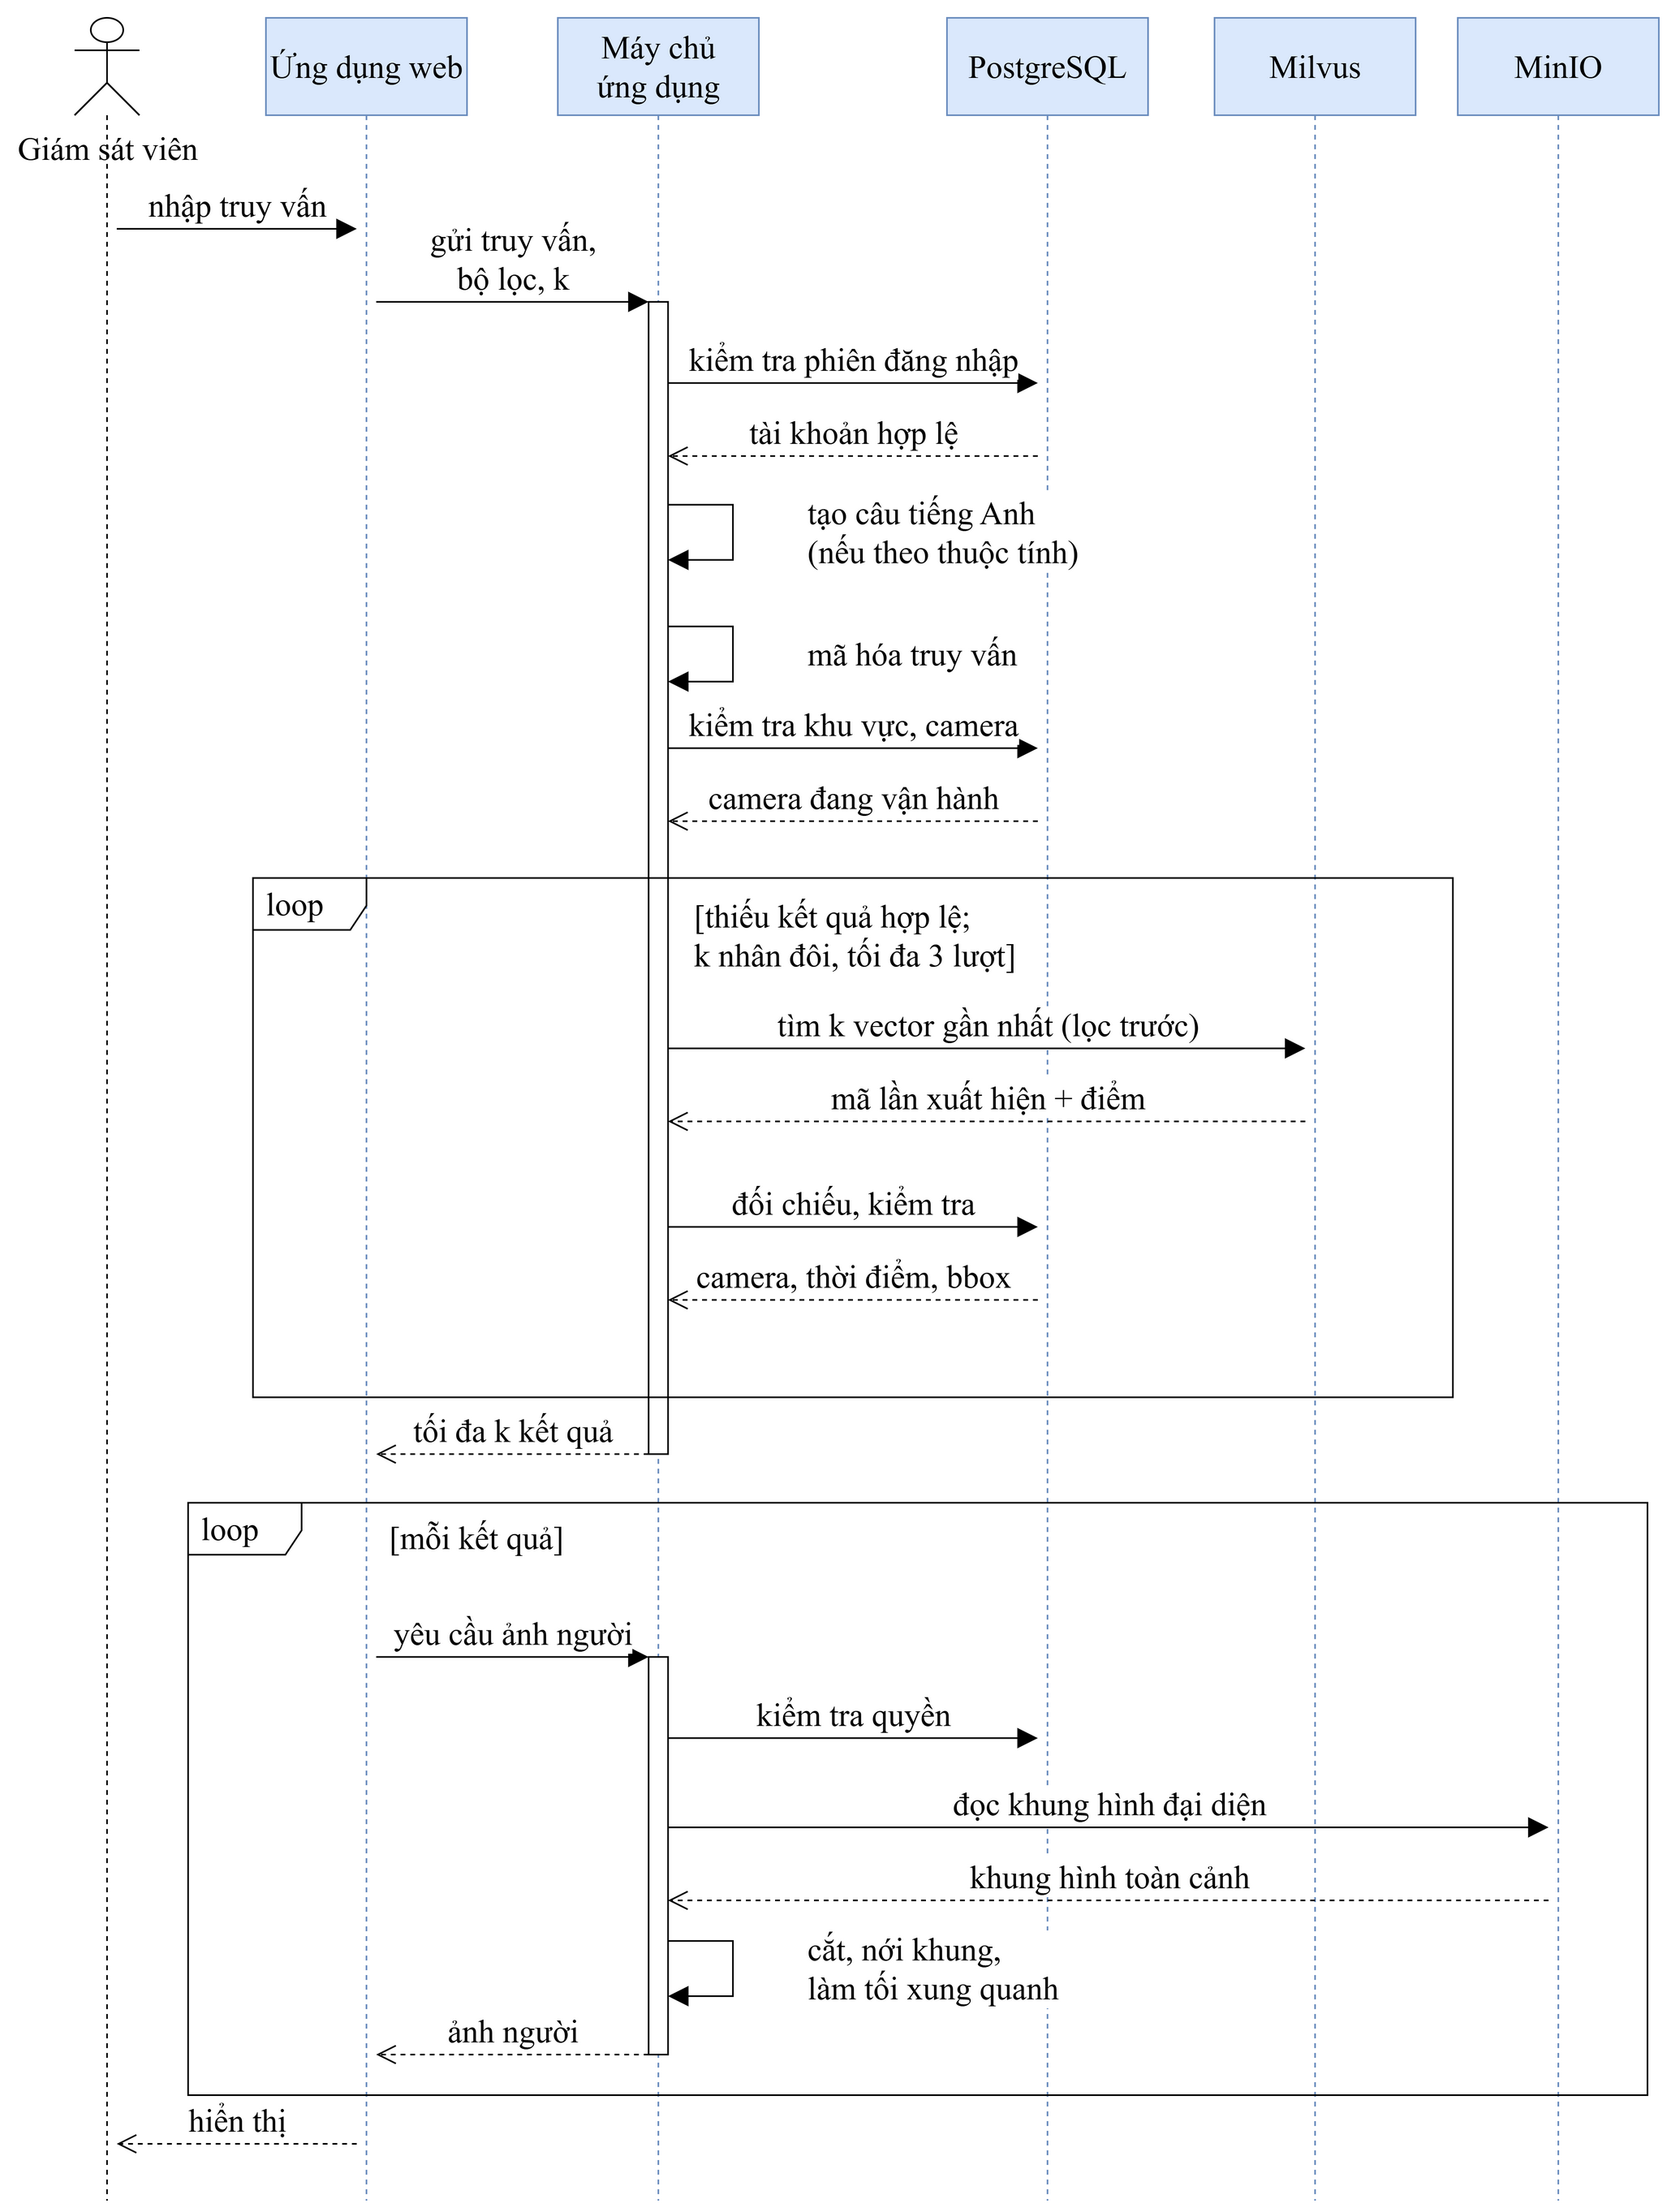
\includegraphics[width=\textwidth]{H4-tuan-tu-tim-kiem.png}
\caption{Sơ đồ tuần tự của luồng tìm kiếm}
\label{fig:search-sequence}
\end{figure}

Ứng dụng web gửi truy vấn cùng bộ lọc camera, khoảng thời gian và số kết quả $k$. Máy chủ ứng dụng lần lượt:
\begin{enumerate}
    \item \textbf{kiểm tra đầu vào:} ảnh JPEG hoặc PNG tối đa 10~MB; thuộc tính thuộc danh sách cho phép và tạo thành tổ hợp hợp lệ; $k$ thuộc tập $\{4, 8, 12, 16\}$;
    \item \textbf{mã hóa truy vấn:} ảnh qua bộ mã hóa ảnh, câu mô tả qua bộ mã hóa văn bản; thuộc tính được ghép thành một câu tiếng Anh theo mẫu cố định, ví dụ \emph{``A woman wearing a red jacket and blue jeans, carrying a handbag.''}, rồi xử lý như câu mô tả;
    \item \textbf{xác định phạm vi:} khu vực lấy từ tài khoản của Giám sát viên; tập camera là các camera được chọn, hoặc mọi camera đang vận hành trong khu vực nếu không chọn; camera ngoài phạm vi bị từ chối;
    \item \textbf{tìm kiếm vector có lọc trước} trong Milvus, đối chiếu kết quả với PostgreSQL và tìm lại với số lượng gấp đôi khi thiếu kết quả hợp lệ, tối đa ba lượt (Mục~\ref{sec:3.6.4}).
\end{enumerate}
Danh sách trả về chỉ chứa thông tin mô tả và điểm phù hợp của từng kết quả. Ảnh được lấy qua một yêu cầu riêng cho từng kết quả, trong đó máy chủ kiểm tra lại quyền rồi dựng ảnh người từ khung hình đại diện (Mục~\ref{sec:6.3.3}). Cách này giúp danh sách được trả về nhanh và mọi ảnh đều đi qua bước kiểm tra quyền.

\subsection{Luồng quản lý hồ sơ vụ việc}
\label{sec:5.2.4}

Hình~\ref{fig:case-sequence} trình bày luồng lưu một kết quả tìm kiếm vào vụ việc mới hoặc vụ việc đã có, với tùy chọn đánh dấu hoàn thành ngay khi lưu.

\begin{figure}[!htbp]
\centering
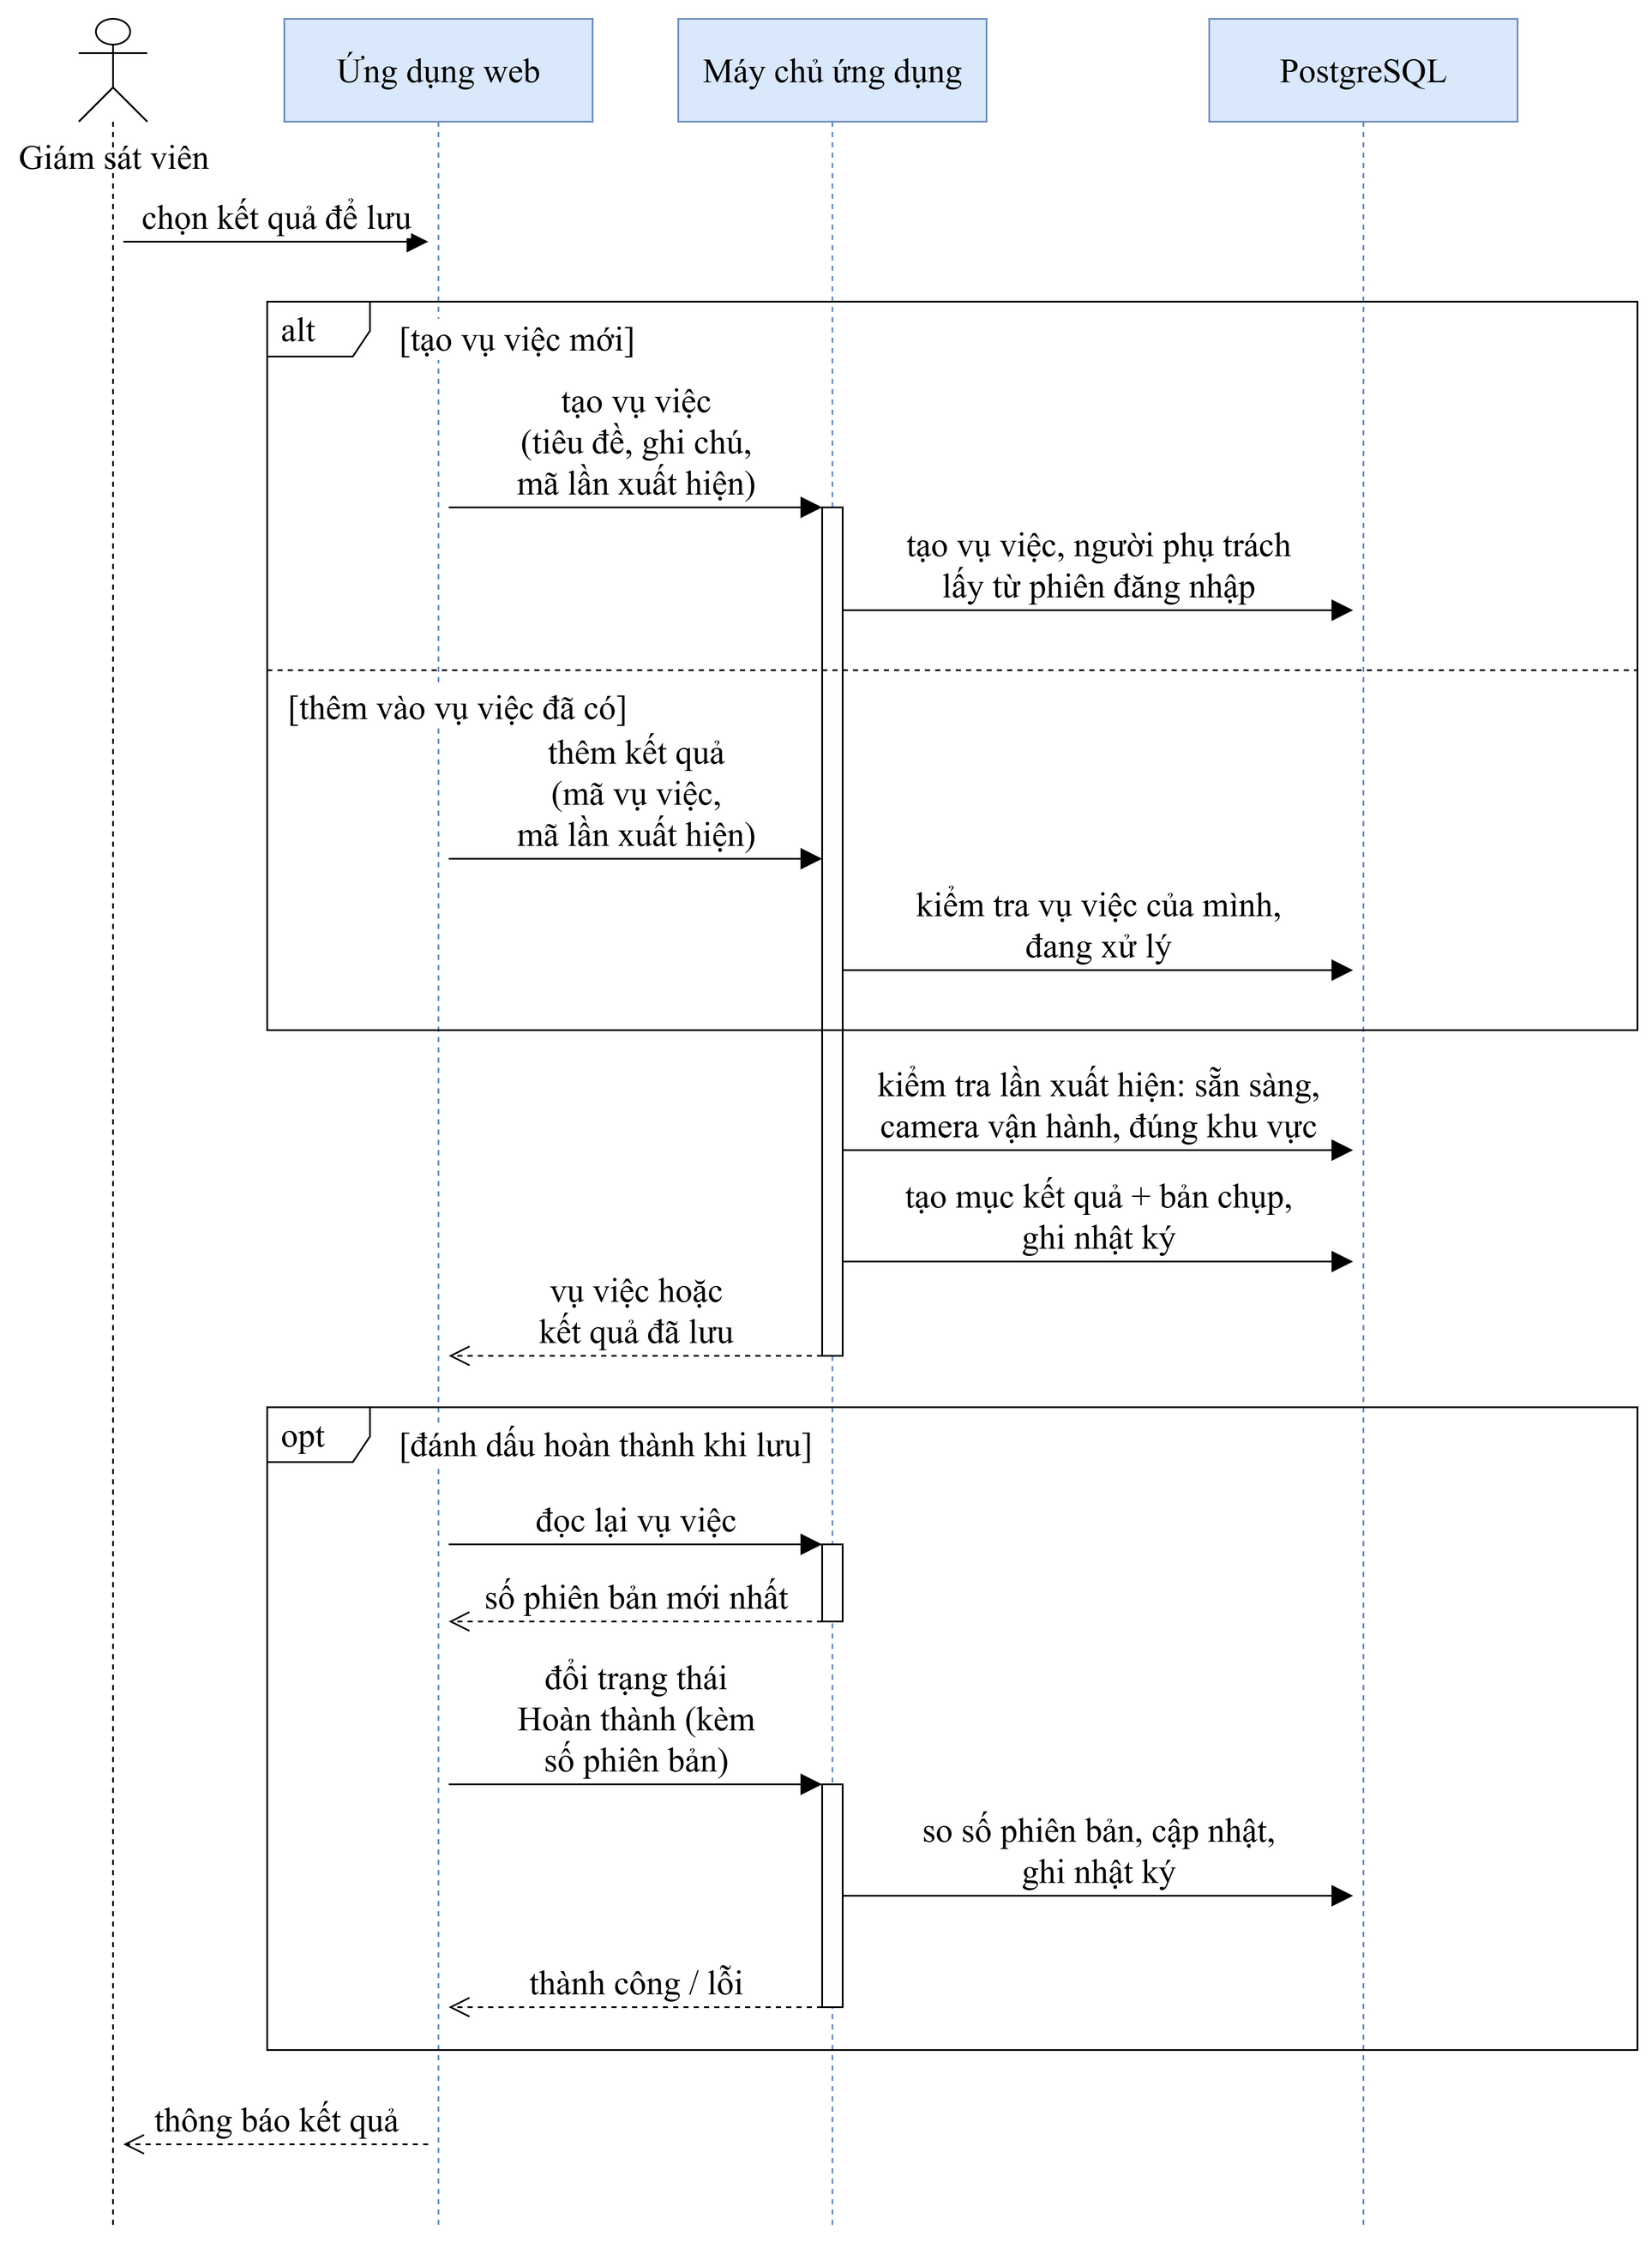
\includegraphics[width=0.95\textwidth]{H5-tuan-tu-vu-viec.png}
\caption{Sơ đồ tuần tự của luồng lưu kết quả vào vụ việc}
\label{fig:case-sequence}
\end{figure}

Khi lưu, giao diện chỉ gửi mã lần xuất hiện, không gửi điểm phù hợp hay thông tin hiển thị. Máy chủ kiểm tra lần xuất hiện đang sẵn sàng và thuộc một camera đang vận hành trong khu vực hiện tại của Giám sát viên, và vụ việc đích do chính người đó phụ trách và đang xử lý. Nếu hợp lệ, máy chủ tạo một mục kết quả mới kèm \emph{bản chụp} tên camera, tên khu vực và thời điểm xuất hiện, để vụ việc vẫn hiển thị đúng khi tên camera thay đổi về sau hoặc khung hình tạm thời không truy xuất được. Mỗi vụ việc mang một số phiên bản; yêu cầu cập nhật phải kèm số phiên bản đang hiển thị, nên thay đổi đồng thời từ nơi khác không bị ghi đè âm thầm. Tùy chọn đánh dấu hoàn thành được giao diện thực hiện sau khi lưu: đọc lại vụ việc để lấy số phiên bản mới nhất, rồi gửi yêu cầu đổi trạng thái kèm số phiên bản đó; nếu yêu cầu đổi trạng thái thất bại, kết quả vẫn được giữ và người dùng được thông báo để đánh dấu lại. Khi mở vụ việc, ảnh được cấp theo quyền đối với vụ việc chứ không theo quyền tìm kiếm (Mục~\ref{sec:4.6}).

% !TEX root = ../../main.tex
% C5.3 — Thiết kế cơ sở dữ liệu (RÚT GỌN 2026-09-29: bỏ 6 bảng từ điển dữ liệu và bảng các bảng vận hành; bản cũ ở report/archive/)
% 5.3.1 khớp backend/src/person_search/storage/postgres/models/*.py và 13 migration (backend/migrations/versions). 12 bảng.
% Bản số trong ERD lấy từ nullable của FK (xem tools/h8_erd_drawio.py). worker_heartbeats không có FK -> không vẽ trong ERD.
% camera "loại khỏi vận hành" = status RETIRED + ai_enabled=false (services/cameras.py); INACTIVE có trong enum nhưng chưa dùng.
% Bất biến areas.code, cameras.area_id và chuyển trạng thái person_tracks được kiểm tra ở tầng ứng dụng (sự kiện before_update của ORM).
% 5.3.2 khớp storage/contracts.py, storage/milvus/vectors.py (7 trường, HNSW/IP M=16 efConstruction=128 ef=64, Strong, upsert).
% 5.3.3 khớp storage/minio/frames.py (JPEG/PNG <= 20 MB, SHA-256, put idempotent), workers/publication.py (JPEG 90), infra/minio (bucket riêng tư).
% 5.3.4 khớp services/track_ingestion.py (PENDING + outbox cùng giao dịch -> MinIO -> Milvus + xác minh -> READY; thử lại 2 s nhân đôi <= 300 s,
% tối đa 5 lần) và storage/maintenance_cli.py (retry-outbox, reconcile mặc định chỉ báo cáo, requeue-track, reindex; chạy thủ công). Hình H6.
\section{Thiết kế cơ sở dữ liệu}
\label{sec:5.3}

\subsection{Cơ sở dữ liệu quan hệ}
\label{sec:5.3.1}

PostgreSQL lưu dữ liệu nghiệp vụ và là nơi quyết định về quyền và trạng thái. 12 bảng của nó chia thành năm nhóm (Bảng~\ref{tab:db-tables}).

\begin{table}[H]
\centering
\caption{Các bảng trong cơ sở dữ liệu quan hệ}
\label{tab:db-tables}
\begin{tabularx}{\textwidth}{|>{\raggedright\arraybackslash}p{3.0cm}|>{\raggedright\arraybackslash}p{5.4cm}|L|}
\hline
\textbf{Nhóm} & \textbf{Bảng} & \textbf{Vai trò} \\
\hline
Tổ chức và phân quyền & \texttt{areas}, \texttt{users}, \path{auth_sessions} & Khu vực giám sát, tài khoản người dùng, phiên đăng nhập \\
\hline
Camera và xử lý AI & \texttt{cameras}, \path{ai_config_versions}, \path{processing_jobs}, \path{worker_heartbeats} & Camera logic, các phiên bản cấu hình Detector-Tracker-bộ mã hóa, hàng đợi công việc, trạng thái tiến trình xử lý nền \\
\hline
Dữ liệu tìm kiếm & \path{person_tracks}, \path{storage_outbox_events} & Thông tin mô tả các lần xuất hiện; sự kiện đồng bộ với hai kho còn lại (Mục~\ref{sec:5.3.4}) \\
\hline
Nghiệp vụ vụ việc & \texttt{cases}, \path{case_results} & Vụ việc và các kết quả đã lưu \\
\hline
Truy vết & \path{audit_logs} & Nhật ký hệ thống, chỉ được thêm, không sửa \\
\hline
\end{tabularx}
\end{table}

Hình~\ref{fig:erd} là sơ đồ thực thể - liên kết của 11 bảng có khóa ngoại theo ký hiệu chân quạ, gồm khóa và các thuộc tính chính; bảng \path{worker_heartbeats} không có khóa ngoại nên không được vẽ.

\afterpage{%
\begin{landscape}
\begin{figure}[p]
\centering
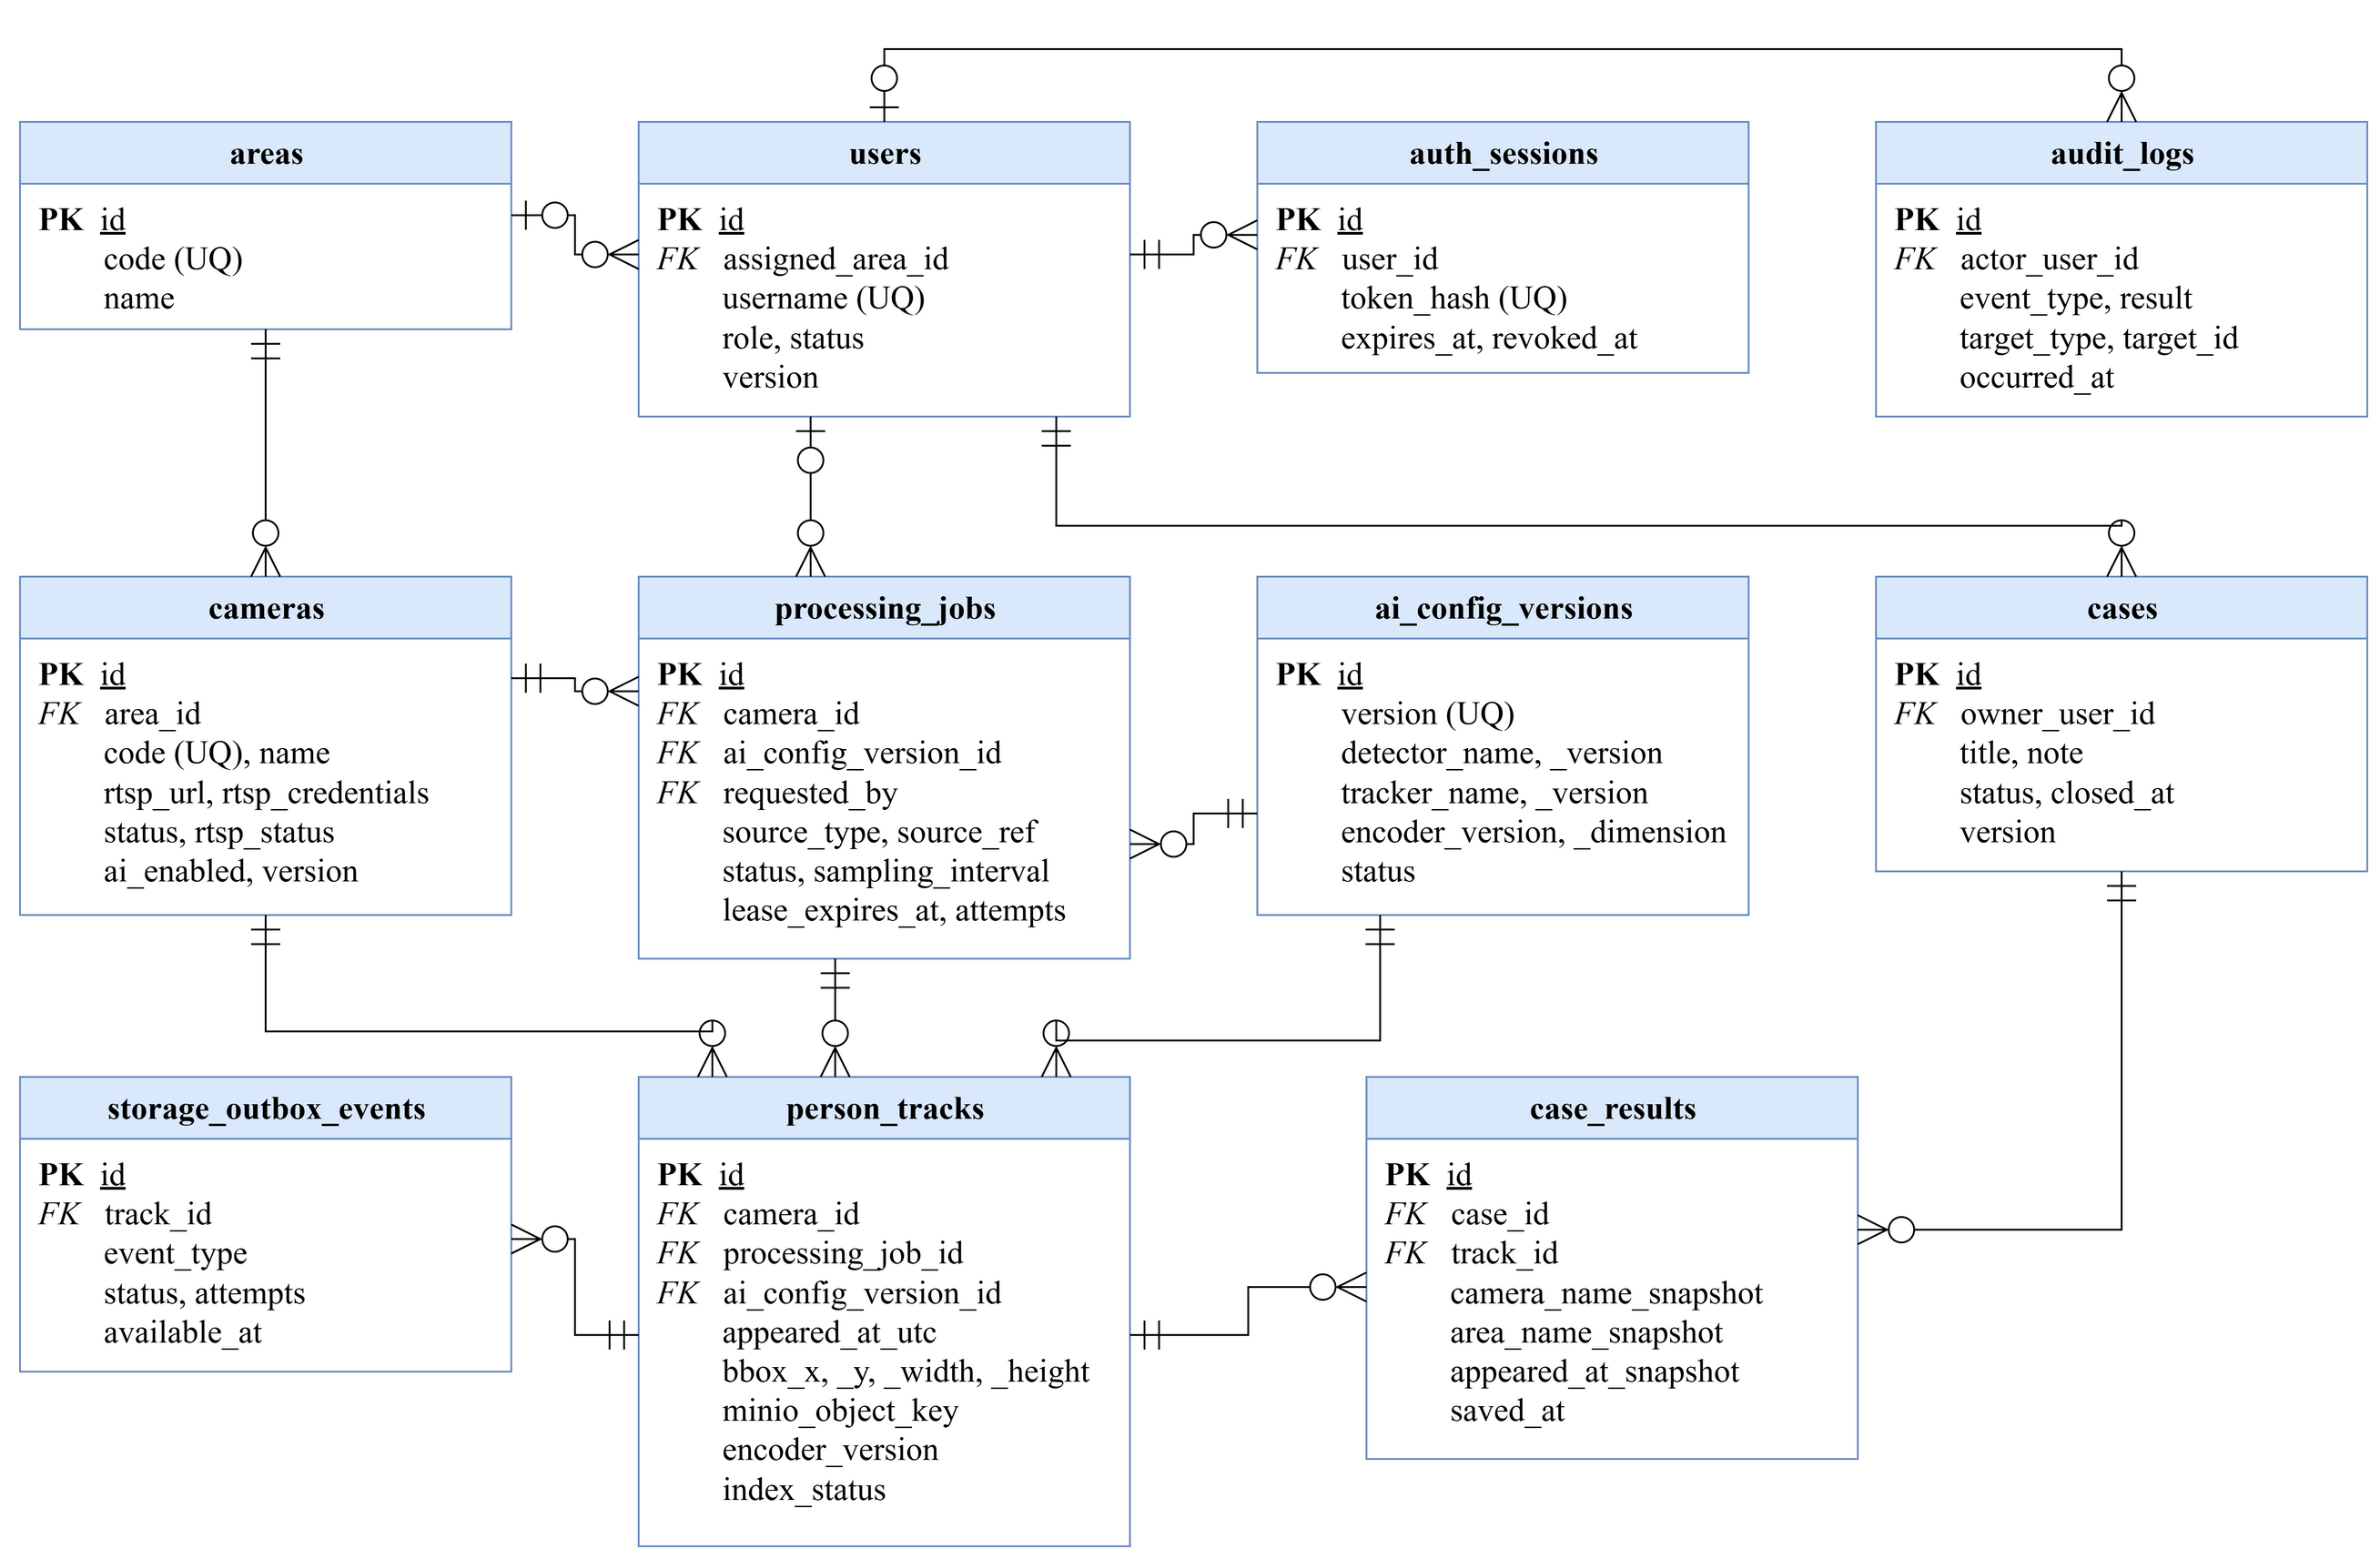
\includegraphics[width=\linewidth,height=0.86\textheight,keepaspectratio]{H8-erd.png}
\caption{Sơ đồ thực thể - liên kết của cơ sở dữ liệu quan hệ}
\label{fig:erd}
\end{figure}
\end{landscape}
}

\paragraph{Các quan hệ.} Phần lớn khóa ngoại là bắt buộc: camera có một khu vực, vụ việc có một người phụ trách, lần xuất hiện có một camera, một công việc và một phiên bản cấu hình AI. Ba khóa ngoại được rỗng: chỉ Giám sát viên có khu vực, chỉ công việc từ tệp tải lên có người yêu cầu, và bản ghi nhật ký như một lỗi kỹ thuật có thể không gắn với người dùng. Giữa \texttt{cases} và \path{person_tracks} là quan hệ nhiều - nhiều qua bảng \path{case_results}. Mỗi dòng của bảng này có khóa chính riêng, lưu bản chụp thông tin tại thời điểm lưu, và \emph{không} có ràng buộc duy nhất trên cặp vụ việc - lần xuất hiện, vì mỗi lần lưu tạo một mục mới.

\paragraph{Các ràng buộc toàn vẹn.} Nhiều quy tắc nghiệp vụ do chính cơ sở dữ liệu ràng buộc, nên lỗi ở tầng ứng dụng không ghi được dữ liệu sai:
\begin{itemize}
    \item Tài khoản Giám sát viên luôn có khu vực, hai vai trò còn lại thì không; vụ việc có thời điểm hoàn thành khi và chỉ khi ở trạng thái \texttt{CLOSED}; chỉ một phiên bản cấu hình AI ở trạng thái \texttt{ACTIVE}; mã khu vực và khu vực của camera không đổi sau khi tạo.
    \item Hầu hết khóa ngoại dùng quy tắc RESTRICT, nên dữ liệu còn được tham chiếu không thể bị xóa; tài khoản và camera không bị xóa dòng mà được chuyển trạng thái (\texttt{INACTIVE}, \texttt{RETIRED}). Chỉ phiên đăng nhập và mục kết quả được xóa theo bảng cha.
    \item Một lần xuất hiện chỉ có thể ở trạng thái \texttt{READY} khi đã có đủ khóa đối tượng, mã băm và kích thước khung hình, và thời điểm ghi vector. Không bảng nào lưu điểm phù hợp.
    \item Các bảng \texttt{users}, \texttt{cameras} và \texttt{cases} có cột số phiên bản để chống ghi đè khi cập nhật đồng thời (Mục~\ref{sec:5.2.4}); cặp người yêu cầu - khóa chống trùng của \path{processing_jobs} là duy nhất, nên một yêu cầu tải lên gửi lặp không tạo thêm công việc.
\end{itemize}
Các chỉ mục phục vụ truy vấn thường gặp như lần xuất hiện theo camera và thời điểm, vụ việc theo người phụ trách, nhật ký theo người thực hiện.

\subsection{Lưu trữ vector đặc trưng}
\label{sec:5.3.2}

Milvus chỉ tìm các vector gần nhất với truy vấn trong một phạm vi đã lọc; mọi thứ khác, kể cả quyền, nằm ở PostgreSQL.

\paragraph{Mỗi phiên bản bộ mã hóa một collection.} Mỗi phiên bản bộ mã hóa có một \emph{collection} (tương tự bảng) riêng trong Milvus, ví dụ \path{person_track_embeddings_rasa_cuhk_pedes_v1}, vì vector của hai phiên bản không so sánh được với nhau. Một bí danh cố định trỏ tới collection đang dùng, và số chiều được kiểm tra khi tiến trình nền khởi động. Mỗi lần xuất hiện ứng với một bản ghi gồm các trường ở Bảng~\ref{tab:milvus-schema}.

\begin{table}[H]
\centering
\caption{Lược đồ collection lưu vector đặc trưng trong Milvus}
\label{tab:milvus-schema}
\begin{tabularx}{\textwidth}{|>{\raggedright\arraybackslash}p{4.2cm}|>{\raggedright\arraybackslash}p{3.7cm}|L|}
\hline
\textbf{Trường} & \textbf{Kiểu} & \textbf{Ý nghĩa} \\
\hline
\path{track_id} & VARCHAR(36), khóa chính & Mã lần xuất hiện, trùng với khóa chính của \path{person_tracks} \\
\hline
\path{embedding} & FLOAT\_VECTOR, 256 chiều & Vector đặc trưng, đã chuẩn hóa L2 \\
\hline
\path{area_id}, \path{camera_id} & VARCHAR(36) & Khu vực và camera, dùng để lọc theo phạm vi \\
\hline
\path{appeared_at_epoch} & INT64 & Thời điểm xuất hiện (giây Unix), dùng để lọc theo thời gian \\
\hline
\path{encoder_version} & VARCHAR(64) & Phiên bản bộ mã hóa đã tạo vector \\
\hline
\path{index_status} & VARCHAR(16) & Trạng thái sẵn sàng; chỉ bản ghi \texttt{READY} được tìm \\
\hline
\end{tabularx}
\end{table}

Khu vực, camera và thời điểm được sao từ PostgreSQL để lọc trước (Mục~\ref{sec:3.6.3}); khu vực của camera không đổi nên bản sao không thể lệch. Trạng thái vận hành thì thay đổi nên không sao chép: mỗi lượt tìm đưa danh sách camera đang vận hành vào điều kiện lọc, nên camera bị loại được ẩn ngay mà không phải sửa Milvus.

\paragraph{Chỉ mục và thao tác.} Trường vector được đánh chỉ mục HNSW với độ đo tích vô hướng, $M = 16$, \textit{ef\-Con\-struc\-tion}~$= 128$, và $\mathit{ef} = 64$ khi tìm (Mục~\ref{sec:3.6.4}). Vector được ghi bằng \emph{upsert} theo mã lần xuất hiện nên thử lại không tạo bản ghi trùng, sau khi kiểm tra số chiều, giá trị và độ dài bằng 1; mức nhất quán mạnh (strong consistency) giúp vector vừa ghi có ngay trong lần tìm tiếp theo.

\subsection{Lưu trữ khung hình}
\label{sec:5.3.3}

Mỗi lần xuất hiện có một tệp trong MinIO là khung hình toàn cảnh đại diện, JPEG chất lượng 90; PostgreSQL lưu khóa đối tượng, mã băm và kích thước. Ảnh người không được lưu mà dựng từ khung hình và khung bao khi cần (Mục~\ref{sec:6.3.3}), nên một tệp phục vụ cả hai cách xem, cách cắt đổi được mà không tạo lại dữ liệu, và không có tệp ảnh người rời. Video gốc không được lưu.

Khóa của mỗi tệp được sinh xác định từ thông tin của lần xuất hiện, theo mẫu
\begin{center}
\texttt{tracks/v1/}\allowbreak \textit{mã camera}\texttt{/}\allowbreak \textit{năm}\texttt{/}\allowbreak \textit{tháng}\texttt{/}\allowbreak \textit{ngày}\texttt{/}\allowbreak \textit{mã lần xuất hiện}\texttt{/}\allowbreak \texttt{representative.jpg}
\end{center}
nên thử lại chỉ ghi đè đúng tệp đó; tiền tố có số phiên bản cho phép đổi cách tổ chức về sau, và nhóm theo camera và ngày giúp dọn dẹp dễ.

Tệp được kiểm tra định dạng, dung lượng (không quá 20~MB) và kích thước, và mã băm SHA-256 lưu ở cả hai kho: trùng khóa cùng mã băm thì dùng lại tệp, khác mã băm là xung đột, và khi đọc mã băm được tính lại để phát hiện tệp hỏng. Bucket là riêng tư, truy cập bằng tài khoản chỉ có quyền trên nó, và không lộ ra trình duyệt.

\subsection{Đảm bảo nhất quán giữa các kho dữ liệu}
\label{sec:5.3.4}

Một lần xuất hiện được lưu thành ba phần ở ba kho không có giao dịch chung, nên việc ghi có thể dừng giữa chừng hoặc một kho có thể tạm không truy cập được. Hệ thống bảo đảm dữ liệu dở dang không xuất hiện trong kết quả, và có thể được hoàn tất hoặc phát hiện về sau.

\paragraph{Trạng thái của lần xuất hiện.} Mỗi lần xuất hiện có một trạng thái đồng bộ với các chuyển trạng thái ở Hình~\ref{fig:track-state}; chỉ lần xuất hiện \emph{Sẵn sàng} mới được tìm, và các chuyển trạng thái khác bị từ chối.

\begin{figure}[!htbp]
\centering
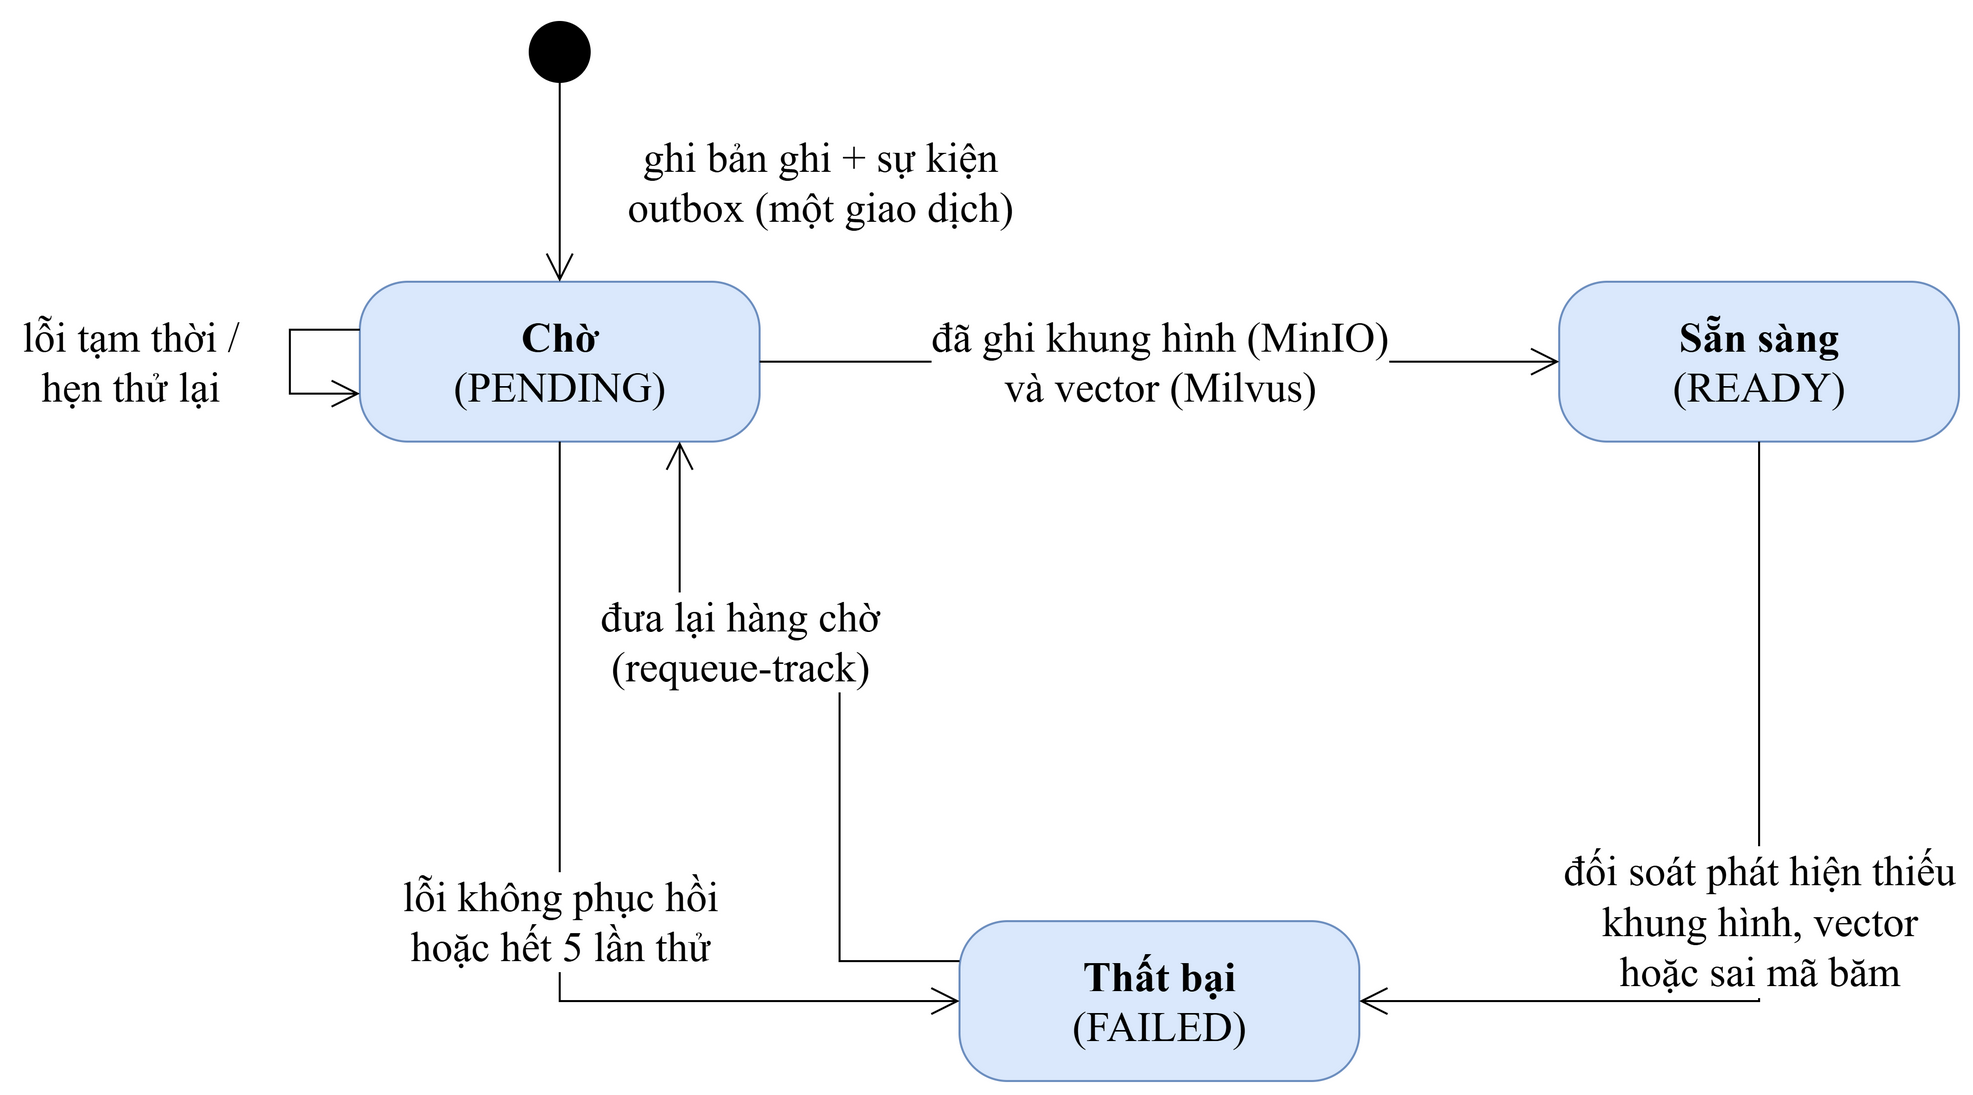
\includegraphics[width=\textwidth]{H6-trang-thai-lan-xuat-hien.png}
\caption{Sơ đồ trạng thái của một lần xuất hiện}
\label{fig:track-state}
\end{figure}

\paragraph{Thứ tự ghi.} Việc ghi một lần xuất hiện theo thứ tự cố định:
\begin{enumerate}
    \item Trong \emph{một giao dịch} của PostgreSQL, tạo bản ghi ở trạng thái \emph{Chờ} và một sự kiện trong bảng \path{storage_outbox_events} lưu đủ những gì cần ghi sang hai kho còn lại, kể cả vector. Đây là mẫu thiết kế \emph{transactional outbox}: ý định ghi sang hệ thống khác được lưu cùng giao dịch với dữ liệu chính.
    \item Ghi khung hình vào MinIO theo khóa xác định.
    \item Ghi vector vào Milvus, rồi đọc lại để xác nhận bản ghi đã tồn tại với đúng khu vực và camera.
    \item Trong một giao dịch mới, chuyển bản ghi sang \emph{Sẵn sàng}, lưu mã băm, kích thước khung hình và thời điểm ghi vector, và đánh dấu sự kiện outbox đã hoàn tất.
\end{enumerate}
Ghi PostgreSQL \emph{trước} nên mọi khung hình và vector đều đối chiếu được với một bản ghi, phần còn lại là dữ liệu mồ côi; đặt \emph{Sẵn sàng} \emph{cuối cùng} nên lần xuất hiện chỉ tìm được khi đủ dữ liệu. Bước 2 và 3 lặp lại an toàn nhờ khóa xác định và upsert.

\paragraph{Xử lý lỗi và công cụ bảo trì.} Lỗi tạm thời ở bước 2 hoặc 3 giữ bản ghi ở \emph{Chờ} và hẹn thử lại, từ 2 giây tăng gấp đôi tới tối đa 300 giây. Sau năm lần, hoặc khi gặp lỗi không phục hồi như xung đột mã băm, bản ghi chuyển sang \emph{Thất bại} và được ghi nhật ký. Vì sự kiện outbox chứa đủ dữ liệu, việc thử lại không phải chạy lại phân tích. Người vận hành có thêm một công cụ dòng lệnh để hoàn tất các lần xuất hiện còn dở, đối soát ba kho nhằm tìm bản ghi chờ quá lâu, bản ghi sẵn sàng nhưng thiếu khung hình hoặc vector, và dữ liệu mồ côi (mặc định chỉ báo cáo; khi được yêu cầu thì cách ly bản ghi hỏng và xóa dữ liệu mồ côi), đưa một lần xuất hiện thất bại về trạng thái chờ, và dựng lại dữ liệu Milvus từ các sự kiện outbox. Các lệnh này hiện được chạy thủ công.

\paragraph{Lớp bảo vệ khi tìm kiếm.} Kể cả khi các kho chưa khớp, người dùng không thấy dữ liệu sai: mỗi kết quả Milvus đều được đối chiếu với PostgreSQL, và kết quả không tồn tại hoặc ngoài phạm vi bị loại (Mục~\ref{sec:3.6.4}).

% !TEX root = ../../main.tex
% C5.4 — Thiết kế giao diện lập trình ứng dụng (API) (RÚT GỌN 2026-09-29: bỏ bảng mã trạng thái HTTP và bảng nhóm API; bản cũ ở report/archive/)
% Khớp backend/src/person_search/api: tiền tố /api/v1 (api/__init__.py), 9 blueprint (api/v1/*.py) + /health (live, ready, storage);
% error_response {"error": {code, message, details, request_id}} (api/errors.py); X-Request-ID; 429 + Retry-After (api/rate_limit.py);
% version trong PATCH users/cameras/cases -> 409 version_conflict; Idempotency-Key khi tải video; tải video trả 202;
% ảnh kết quả tìm kiếm /search-results/{id}/crop|frame, ảnh kết quả đã lưu /cases/{id}/results/{id}/crop|frame.
\section{Thiết kế giao diện lập trình ứng dụng}
\label{sec:5.4}

Ứng dụng web và máy chủ ứng dụng giao tiếp hoàn toàn qua một giao diện lập trình ứng dụng (API) theo phong cách REST. Mọi API nghiệp vụ nằm dưới tiền tố \path{/api/v1} và gọi tên tài nguyên bằng danh từ số nhiều, như \path{/cases}. Các API chỉ dành cho Quản trị viên nằm dưới \path{/admin}. Dữ liệu trao đổi ở dạng JSON, riêng ảnh truy vấn và tệp video được gửi dạng \texttt{multipart/form-data}. Các thao tác chuyển trạng thái có ý nghĩa nghiệp vụ, như khóa tài khoản hay loại camera khỏi vận hành, được thiết kế thành hành động tường minh, ví dụ \texttt{POST} \path{/admin/cameras/{id}/retire}, để mỗi thao tác được kiểm tra điều kiện và ghi nhật ký riêng.

Mọi lỗi được trả về theo một định dạng thống nhất gồm \emph{mã lỗi} ổn định để giao diện xử lý theo chương trình, \emph{thông báo} tiếng Việt để hiển thị, \emph{chi tiết} như lỗi của từng trường, và \emph{mã yêu cầu} để đối chiếu với nhật ký máy chủ. Mã trạng thái HTTP được dùng theo ý nghĩa chuẩn: 401 khi chưa đăng nhập hoặc phiên hết hạn, 403 khi vai trò không được phép, 404 khi tài nguyên không tồn tại hoặc nằm ngoài phạm vi được phép, 409 khi xung đột với trạng thái hiện tại, 422 khi dữ liệu không hợp lệ và 429 khi vượt giới hạn số lần gọi.

Để chống ghi đè, yêu cầu cập nhật tài khoản, camera và vụ việc phải kèm số phiên bản mà giao diện đang có. Nếu dữ liệu đã bị thay đổi ở nơi khác, máy chủ trả mã 409 thay vì ghi đè. Yêu cầu tải video có thể kèm một khóa chống lặp, nên gửi lại không tạo thêm công việc. Tải video lên cũng là một tác vụ không đồng bộ: máy chủ chỉ tạo công việc và trả mã 202 ngay, còn giao diện theo dõi tiến độ qua API công việc thay vì giữ yêu cầu mở trong suốt quá trình phân tích.

Về phân quyền, không API nào nhận khu vực của Giám sát viên hay người phụ trách vụ việc làm tham số. Máy chủ tự xác định các giá trị này từ phiên đăng nhập, nên việc sửa yêu cầu ở trình duyệt không thể mở rộng quyền. Phản hồi tìm kiếm và phản hồi xem vụ việc chỉ chứa thông tin mô tả, còn ảnh được lấy qua các đường dẫn riêng. Ảnh của kết quả tìm kiếm và ảnh của kết quả đã lưu dùng hai bộ đường dẫn khác nhau, ứng với hai căn cứ quyền xem ảnh ở Mục~\ref{sec:4.6}.

Ngoài các API nghiệp vụ, máy chủ có ba đường dẫn kiểm tra tình trạng (\path{/health/live}, \path{/health/ready}, \path{/health/storage}) phục vụ việc triển khai và giám sát.

% !TEX root = ../../main.tex
% C5.5 — Thiết kế bảo mật và phân quyền (RÚT GỌN 2026-09-29: bảng giới hạn tần suất -> câu văn; gộp 5.5.4 + 5.5.5; bản cũ ở report/archive/)
% Khớp: auth/tokens.py (mã phiên 32 byte ngẫu nhiên, lưu SHA-256; CSRF = HMAC-SHA256(mã phiên, ngữ cảnh)); auth/web.py (cookie HttpOnly, SameSite=Lax,
% Secure ở môi trường chính thức; tiêu đề X-CSRF-Token cho phương thức không an toàn; require_auth(vai trò) -> 403);
% auth/passwords.py (Argon2, dài tối thiểu 8, băm giả khi không có tài khoản); services/auth.py (login thu hồi phiên cũ; mỗi yêu cầu kiểm tra thu hồi,
% hạn 12 h, 30 phút không hoạt động, tài khoản ACTIVE, Operator có khu vực; refresh cấp mã mới); api/security.py (CORS danh sách cho phép, tiêu đề bảo mật);
% api/rate_limit.py + config.py (login 10 theo IP + tên, search 30, upload 10, connection_test 10, diagnostics 6 mỗi phút; bộ đếm trong bộ nhớ);
% services/cases.py (không phải chủ -> 404); services/camera_runtime.py (Fernet, chỉ IP literal thuộc dải cho phép, chặn loopback/link-local/multicast).
% LƯU Ý: refresh() đặt hạn mới = now + 12 h -> hạn 12 h không còn "tuyệt đối" khi người dùng hoạt động liên tục (architect.md §13 #8). Văn bản mô tả đúng code.
\section{Thiết kế bảo mật và phân quyền}
\label{sec:5.5}

Các yêu cầu bảo mật ở Mục~\ref{sec:4.3.1} và ma trận phân quyền ở Mục~\ref{sec:4.6} được hiện thực theo nguyên tắc \emph{phòng thủ nhiều lớp}: mỗi yêu cầu được kiểm tra phiên, vai trò và phạm vi dữ liệu, và ràng buộc cơ sở dữ liệu là lớp cuối cùng.

\subsection{Xác thực và phiên đăng nhập}
\label{sec:5.5.1}

Mật khẩu dài tối thiểu 8 ký tự và được băm bằng Argon2. Tên đăng nhập không tồn tại vẫn được kiểm tra trên một giá trị băm giả và nhận cùng thông báo như sai mật khẩu, nên thời gian phản hồi và nội dung lỗi không cho biết tên nào tồn tại.

Đăng nhập thành công tạo một mã phiên ngẫu nhiên 32 byte trong cookie \texttt{HttpOnly} (mã JavaScript không đọc được), \texttt{SameSite=Lax} (không gửi kèm yêu cầu thay đổi dữ liệu từ trang khác) và \texttt{Secure} khi chạy qua HTTPS. Cơ sở dữ liệu chỉ lưu mã băm SHA-256 của mã phiên, nên bảng phiên bị lộ cũng không chứa mã hợp lệ. Yêu cầu nhận 401 nếu phiên đã bị thu hồi, quá 12 giờ kể từ khi cấp hoặc quá 30 phút không hoạt động, và phiên bị thu hồi ngay nếu tài khoản bị khóa, ngừng hoạt động hoặc là Giám sát viên không còn khu vực. Khi người dùng còn thao tác, giao diện làm mới phiên; mỗi lần làm mới cấp mã mới với hạn 12 giờ riêng và thu hồi mã cũ, nên mã bị lộ chỉ có giá trị trong thời gian ngắn.

\subsection{Chống giả mạo yêu cầu}
\label{sec:5.5.2}

Vì trình duyệt tự gửi cookie, một trang web khác có thể khiến nó gửi yêu cầu tới hệ thống (CSRF). Ngoài \texttt{SameSite}, mọi yêu cầu thay đổi dữ liệu phải kèm tiêu đề \texttt{X-CSRF-Token}, là HMAC-SHA256 của mã phiên được trả cho giao diện khi đăng nhập, mà trang khác không đọc được. Chỉ các nguồn được cấu hình mới gọi được API kèm cookie (CORS), và phản hồi kèm các tiêu đề bảo mật cấm đoán kiểu nội dung, cấm nhúng trang và không lưu bộ nhớ đệm.

\subsection{Phân quyền}
\label{sec:5.5.3}

Phân quyền có ba lớp tại máy chủ. Mỗi API khai báo vai trò được phép và từ chối vai trò khác với mã 403 trước mọi xử lý. Tầng nghiệp vụ kiểm tra từng đối tượng: camera và lần xuất hiện thuộc khu vực hiện tại của Giám sát viên và đang vận hành, vụ việc do chính người đó phụ trách, ảnh theo một trong hai căn cứ ở Mục~\ref{sec:4.6}; khu vực và người phụ trách luôn lấy từ phiên chứ không từ yêu cầu, nên sửa yêu cầu ở trình duyệt không mở rộng được quyền. Cuối cùng, ràng buộc cơ sở dữ liệu chặn dữ liệu sai kể cả khi tầng nghiệp vụ có lỗi.

Đối tượng ngoài phạm vi nhận 404 thay vì 403, để việc thử lần lượt các mã không cho biết đối tượng nào tồn tại.

\subsection{Bảo vệ dữ liệu và hạn chế lạm dụng}
\label{sec:5.5.4}

Thông tin xác thực RTSP được tách khỏi địa chỉ, mã hóa bằng Fernet với khóa từ biến môi trường và chỉ giải mã khi kết nối; nó không bao giờ được trả về hay ghi nhật ký. Vì kiểm tra kết nối khiến máy chủ kết nối tới địa chỉ do người dùng nhập, chỉ địa chỉ IP thuộc dải mạng camera đã khai báo được chấp nhận, còn loopback, link-local và multicast luôn bị từ chối, để chức năng này không bị dùng dò mạng nội bộ (SSRF).

Các chức năng tốn tài nguyên hoặc dễ bị dò được giới hạn mỗi phút: đăng nhập 10 lần theo cặp IP - tên đăng nhập, và theo tài khoản: tìm kiếm 30, tải video 10, kiểm tra kết nối 10, kiểm tra AI 6 lần; vượt giới hạn thì nhận 429 kèm thời gian chờ. Bộ đếm nằm trong bộ nhớ tiến trình, phù hợp triển khai một tiến trình. Ảnh truy vấn phải là JPEG hoặc PNG, không quá 10~MB và 24 triệu điểm ảnh, video không quá 500~MB và có chữ ký định dạng hợp lệ, và tên tệp người dùng gửi không dùng làm đường dẫn lưu trữ.

% !TEX root = ../../main.tex
% C5.6 — Thiết kế giao diện người dùng (RÚT GỌN 2026-09-29; bỏ nguyên tắc "ngôn ngữ nhất quán" vì trùng NFR-19; bản cũ ở report/archive/)
% Khớp frontend/src: constants/navigation.js (menu theo vai trò, HOME_BY_ROLE), routes/AppRoutes.jsx + guards.jsx,
% features/results/ResultViewer.jsx, CreateCaseDialog, AddToCaseDialog, features/search/ImageDropzone.jsx, SearchResults.jsx,
% components/person/PersonCrop.jsx, pages/viewer/OverviewPage.jsx; architect §9 (dùng được ở 390 px). Hình H12.
\section{Thiết kế giao diện người dùng}
\label{sec:5.6}

Giao diện được thiết kế trực tiếp trên ứng dụng web, không qua bước bản mẫu; Mục~\ref{sec:6.3} trình bày các màn hình chính.

\subsection{Cấu trúc màn hình theo vai trò}
\label{sec:5.6.1}

Mỗi vai trò vào trang chủ riêng và chỉ thấy màn hình của mình (Hình~\ref{fig:screen-flow}). Trong hình, mũi tên đậm chỉ trang mở sau khi đăng nhập, khung nét đứt là hộp thoại, còn các màn hình cùng vai trò nối với nhau qua menu bên trái.

\begin{figure}[!htbp]
\centering
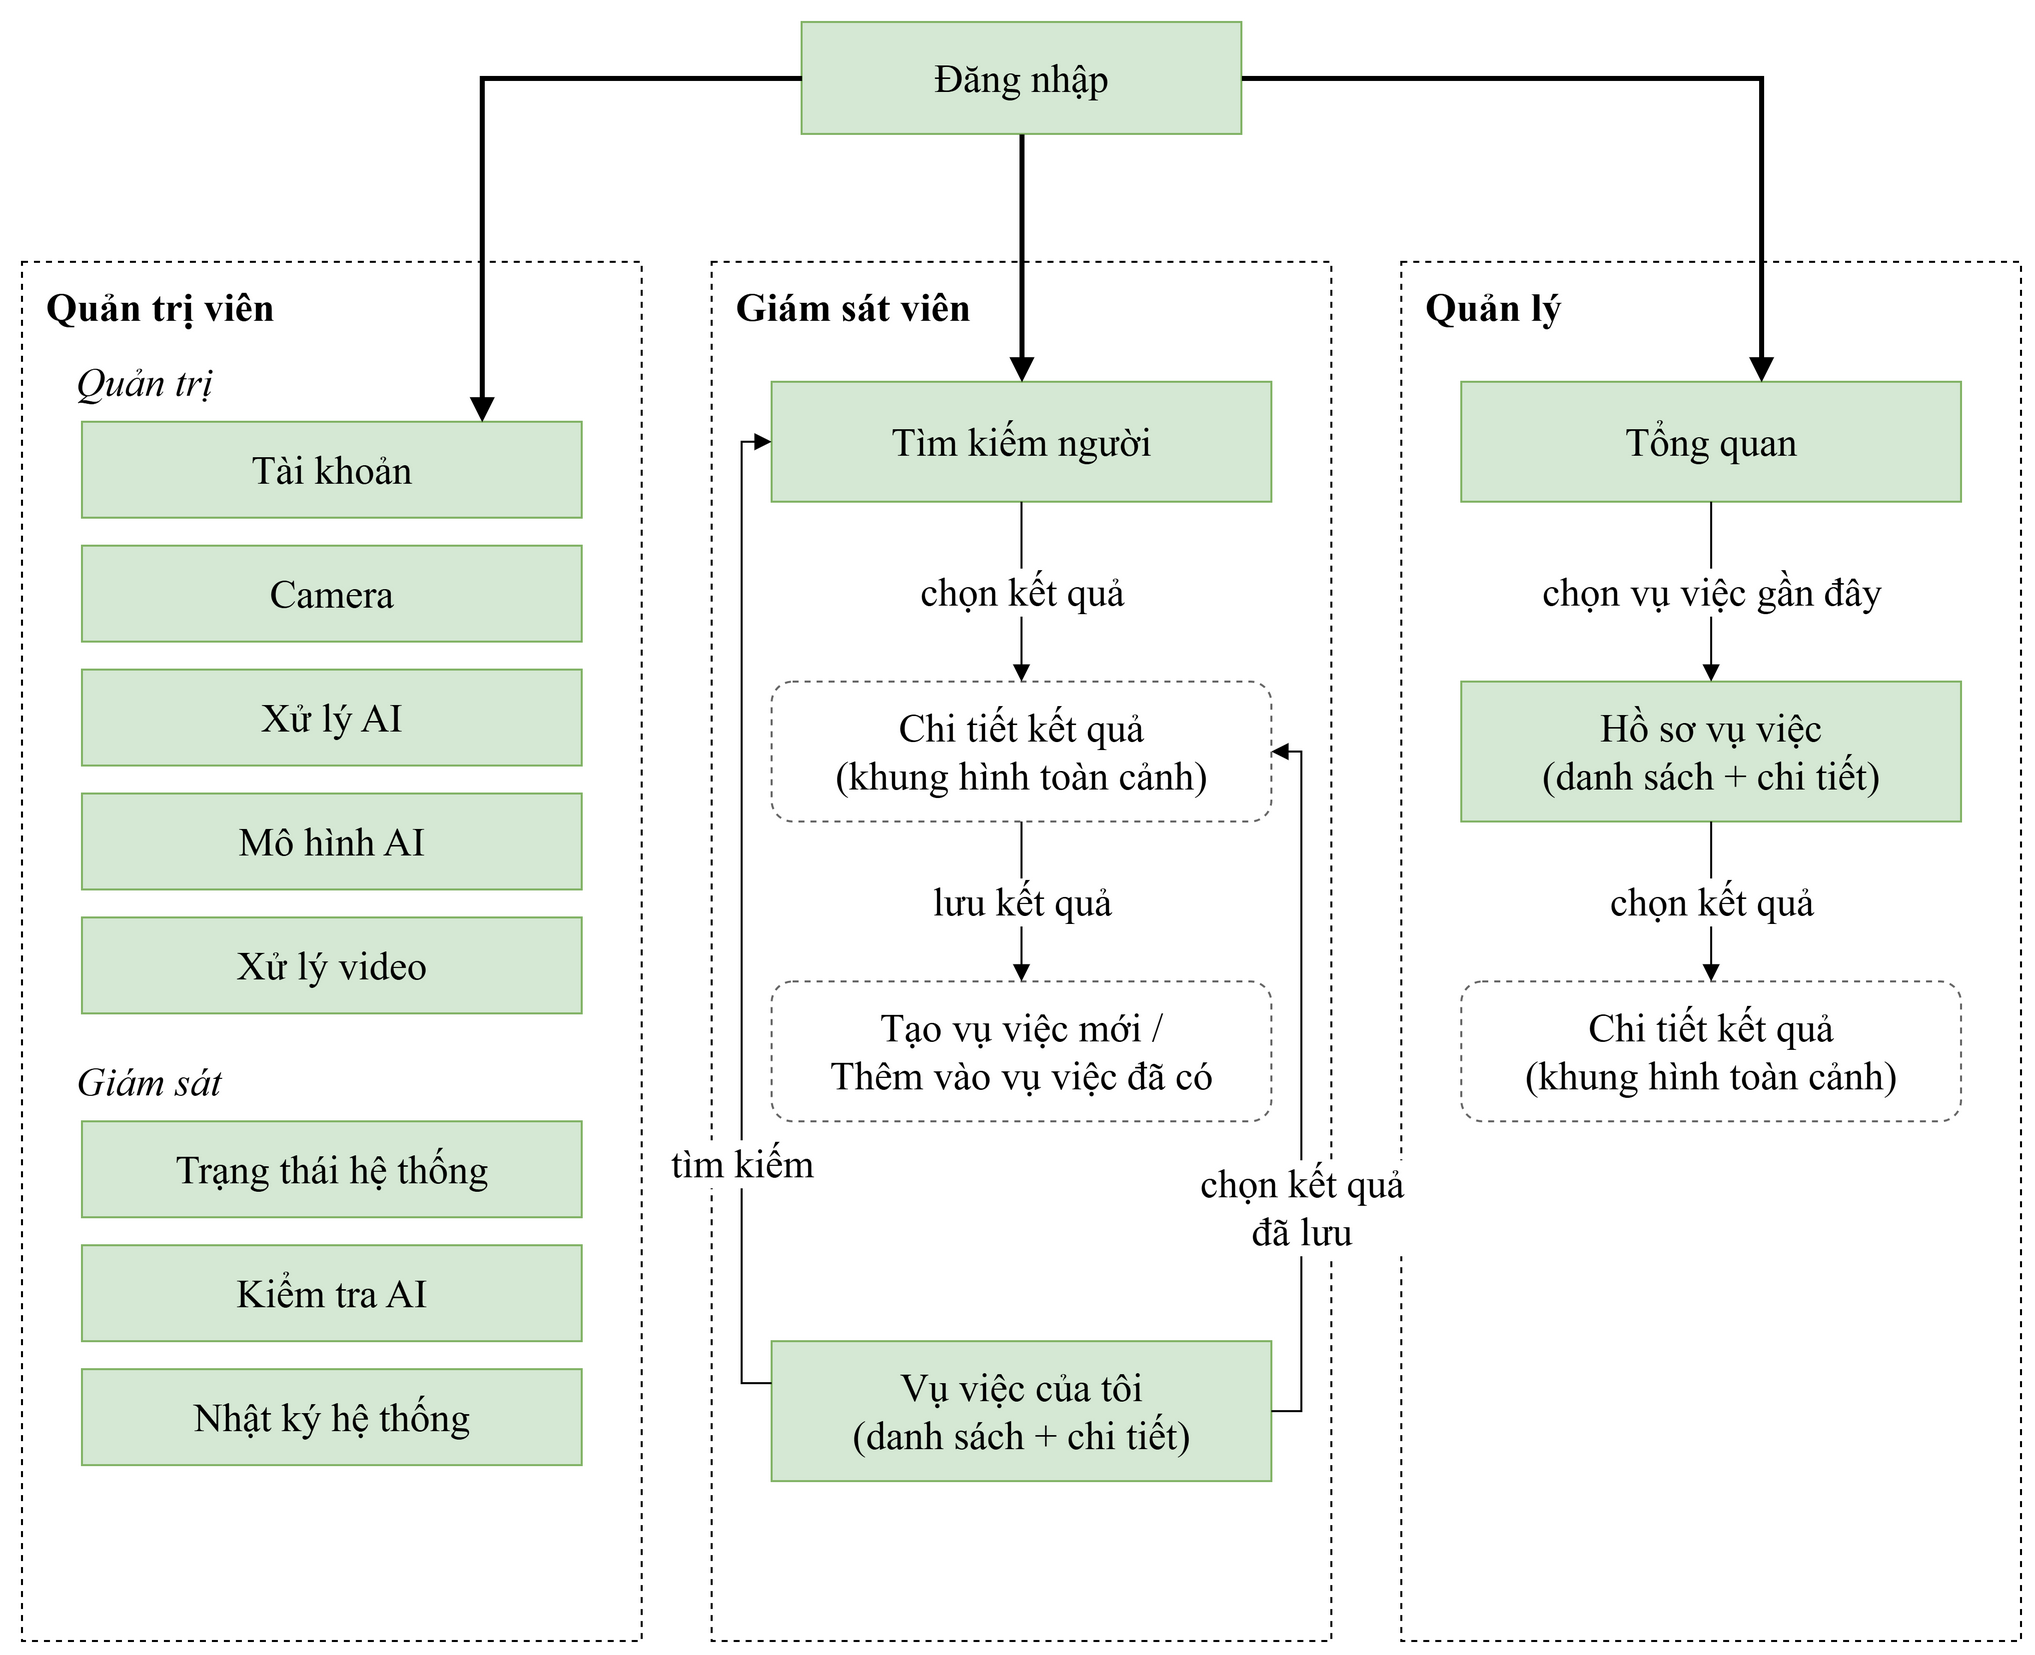
\includegraphics[width=\textwidth]{H12-luong-man-hinh.png}
\caption{Sơ đồ luồng màn hình theo vai trò}
\label{fig:screen-flow}
\end{figure}

\begin{itemize}
    \item \textbf{Quản trị viên} có tám màn hình trong hai nhóm \emph{Quản trị} và \emph{Giám sát}.
    \item \textbf{Giám sát viên} làm việc chủ yếu trên \emph{Tìm kiếm người}, nơi biểu mẫu và kết quả cùng một trang để tìm lại nhiều lần; một kết quả mở hộp thoại chi tiết, từ đó lưu vào vụ việc. \emph{Vụ việc của tôi} gồm danh sách và chi tiết trên cùng một trang.
    \item \textbf{Quản lý} bắt đầu từ \emph{Tổng quan} và mở vụ việc ở \emph{Hồ sơ vụ việc}, là bản chỉ đọc của màn hình vụ việc của Giám sát viên.
\end{itemize}

\subsection{Các nguyên tắc thiết kế}
\label{sec:5.6.2}

Vì mọi kết quả đều cần người dùng xác nhận, giao diện trước hết hỗ trợ đánh giá bằng mắt (NFR-20): ảnh người đặt trong khung hình, người được tìm thấy được làm nổi bật khi có nhiều người, thứ hạng, camera và giờ xuất hiện được ưu tiên, còn điểm phù hợp chỉ là thông tin phụ.

Giao diện cũng giảm thao tác lặp: ảnh truy vấn đưa vào được nhiều cách, kể cả kéo một kết quả vào ô tìm kiếm (FR-O01), và kết quả sắp xếp, lọc lại được mà không cần truy vấn mới.

Khi không có kết quả, giao diện nêu lý do và gợi ý cách tiếp tục; lỗi dùng thông báo tiếng Việt của máy chủ, và khi dữ liệu đã đổi ở nơi khác thì người dùng được yêu cầu tải lại. Trên điện thoại rộng khoảng 390 điểm ảnh, menu trái thành danh sách chọn và bảng rộng được cuộn ngang.


% !TEX root = ../../main.tex
% Chương 6 — xem mục C6 trong report/report_plan.md
\chapter{Hiện thực hệ thống}
\label{chapter:hienthuc}

\textit{Chương này trình bày việc đánh giá, lựa chọn công nghệ và mô hình, cách hiện thực tiến trình xử lý nền AI và giao diện người dùng, cùng các công cụ giám sát vận hành.}

% !TEX root = ../../main.tex
% C6.1 — Đánh giá và lựa chọn công nghệ, mô hình (RÚT GỌN 2026-09-29; bản cũ ở report/archive/)
% Phiên bản lấy từ frontend/package.json, backend/pyproject.toml + requirements lock, infra/compose.yaml.
% Lịch sử lựa chọn: architect.md mục 9, 12 (FastAPI + pgvector + tệp cục bộ được gợi ý ban đầu -> Flask + Milvus + MinIO + PostgreSQL;
% RaSa theo đề xuất của giảng viên; CLIP đa ngôn ngữ từng được cân nhắc; OpenVINO để sau). AI plan: YOLOX dự phòng giấy phép (đăng ký, chưa có trọng số).
% Số liệu YOLO11 lấy từ docs.ultralytics.com/models/yolo11 (đã kiểm chứng). pgvector: lọc sau khi quét chỉ mục (README chính thức).
% 3.2 dẫn sec:6.1.4 (lý do chọn YOLO11n); 3.6 dẫn sec:6.1.3 (lý do chọn Milvus).
\section{Đánh giá và lựa chọn công nghệ, mô hình}
\label{sec:6.1}

Các lựa chọn được đánh giá theo bốn tiêu chí: yêu cầu ở Chương~\ref{chapter:phantich}; chạy được trên máy chỉ có CPU và 16~GB bộ nhớ; mã nguồn mở với giấy phép phù hợp đồ án phi thương mại; và mức quen thuộc của tác giả, để giảm rủi ro. Bảng~\ref{tab:tech-summary} tóm tắt các lựa chọn; các lựa chọn chính được giải thích dưới đây.

\begin{table}[H]
\centering
\caption{Tóm tắt các lựa chọn công nghệ và mô hình}
\label{tab:tech-summary}
\begin{tabularx}{\textwidth}{|>{\raggedright\arraybackslash}p{3.0cm}|>{\raggedright\arraybackslash}p{3.1cm}|>{\raggedright\arraybackslash}p{3.4cm}|L|}
\hline
\textbf{Thành phần} & \textbf{Lựa chọn} & \textbf{Phương án đã cân nhắc} & \textbf{Lý do chính} \\
\hline
Giao diện & React 19, Vite, Tailwind CSS & Sinh trang ở máy chủ; Angular, Vue & Nhiều tương tác trên một màn hình; tách giao diện và máy chủ qua API \\
\hline
Máy chủ & Python, Flask 3.1, SQLAlchemy, Alembic & Django, FastAPI & Cùng ngôn ngữ với các mô hình AI; gọn, tường minh \\
\hline
Hàng đợi & Bảng trong PostgreSQL & Celery kèm Redis hoặc RabbitMQ & Một tiến trình xử lý tuần tự; ít thành phần hạ tầng \\
\hline
CSDL quan hệ & PostgreSQL 17 & MySQL & Ràng buộc CHECK, chỉ mục có điều kiện, JSONB, \texttt{SKIP LOCKED} \\
\hline
Lưu trữ vector & Milvus 2.6 & pgvector, FAISS & Lọc trước khi tìm, lưu trữ bền vững, tách collection theo phiên bản \\
\hline
Lưu trữ khung hình & MinIO & Tệp trên ổ đĩa & Phân quyền theo bucket, mã băm, dùng chung với Milvus \\
\hline
Phát hiện người & YOLO11n & YOLO11s, YOLO11m, YOLOX, Faster R-CNN & Nhanh nhất trên CPU; YOLOX dự phòng về giấy phép \\
\hline
Theo vết & ByteTrack (mặc định), BoT-SORT & DeepSORT, StrongSORT & Không cần đặc trưng ngoại hình cho mỗi người mỗi khung hình \\
\hline
Bộ mã hóa & RaSa & Hai mô hình riêng; CLIP & Một không gian chung cho ba hình thức truy vấn \\
\hline
\end{tabularx}
\end{table}

\subsection{Công nghệ phía giao diện}
\label{sec:6.1.1}

Giao diện có nhiều tương tác trên một màn hình, như kéo thả ảnh truy vấn, sắp xếp lại kết quả hay mở hộp thoại chồng lên danh sách, nên phù hợp hướng \emph{ứng dụng một trang}: tải một lần rồi chỉ trao đổi dữ liệu qua API. Đề tài chọn React nhờ hệ sinh thái thư viện điều hướng, gọi API và định kiểu, cùng Vite để đóng gói và Tailwind CSS cho bố cục thống nhất, co giãn trên điện thoại.

\subsection{Công nghệ phía máy chủ}
\label{sec:6.1.2}

Máy chủ và tiến trình nền viết bằng Python, ngôn ngữ của mọi mô hình trong đề tài, nên máy chủ nạp trực tiếp được bộ mã hóa truy vấn và dùng chung mã truy cập dữ liệu với tiến trình nền. Django nặng hơn nhu cầu của một máy chủ chỉ có API, còn lợi thế bất đồng bộ của FastAPI không đáng kể khi phân tích video đã tách khỏi máy chủ (Mục~\ref{sec:5.1.3}); Flask gọn, tường minh và tác giả đã quen dùng. Với một tiến trình xử lý tuần tự, một bảng PostgreSQL thay cho Celery cùng Redis hay RabbitMQ, tiết kiệm bộ nhớ trên máy triển khai.

\subsection{Hệ quản trị cơ sở dữ liệu và lưu trữ}
\label{sec:6.1.3}

PostgreSQL có những tính năng thiết kế dùng trực tiếp: ràng buộc CHECK phức tạp, chỉ mục có điều kiện, JSONB cho nhật ký và số đo, và \texttt{SKIP LOCKED} để nhận công việc an toàn. Với vector, pgvector~\cite{pgvector2026} chỉ cần một cơ sở dữ liệu nhưng với chỉ mục gần đúng thì lọc \emph{sau} khi quét nên có thể trả thiếu kết quả (Mục~\ref{sec:3.6.3}); FAISS là thư viện trong bộ nhớ, để ứng dụng tự lo lưu trữ, lọc và truy cập đồng thời. Milvus~\cite{wang2021milvus} lọc trước khi tìm~\cite{milvus2026filtered}, đáp ứng trực tiếp phân quyền theo khu vực; nó cần thêm etcd và kho đối tượng, nhưng toàn bộ dịch vụ trong Docker chỉ dùng khoảng 515~MiB bộ nhớ (Mục~\ref{sec:8.7}). Khung hình lưu trong MinIO thay vì tệp thường để kiểm soát quyền theo bucket và lưu mã băm từng đối tượng, dùng chung máy chủ MinIO mà Milvus vốn cần, ở bucket riêng.

\subsection{Các mô hình AI}
\label{sec:6.1.4}

\paragraph{Phát hiện người.} Hướng hai giai đoạn như Faster R-CNN quá chậm trên CPU, nên đề tài chọn họ YOLO. Trong YOLO11, kích cỡ quyết định tốc độ trên CPU (Bảng~\ref{tab:yolo11-sizes}), và ngay YOLO11n đã khiến quy trình chậm hơn thời gian thực khoảng bảy lần (Mục~\ref{sec:7.2}), nên đề tài chọn kích cỡ nhỏ nhất, bù độ chính xác bằng ngưỡng tin cậy thấp kết hợp theo vết. Giấy phép AGPL-3.0 của YOLO11 phù hợp đồ án phi thương mại nhưng không phù hợp sản phẩm, nên YOLOX~\cite{ge2021yolox} (Apache-2.0) được đăng ký làm dự phòng.

\begin{table}[H]
\centering
\caption{So sánh các kích cỡ YOLO11 trên tập kiểm định COCO~\cite{ultralytics2024yolo11docs}}
\label{tab:yolo11-sizes}
\begin{tabularx}{\textwidth}{|L|>{\raggedright\arraybackslash}p{2.6cm}|>{\raggedright\arraybackslash}p{3.8cm}|>{\raggedright\arraybackslash}p{3.0cm}|}
\hline
\textbf{Mô hình} & \textbf{mAP$_{50\text{--}95}$} & \textbf{Thời gian trên CPU (ms/ảnh)} & \textbf{Số tham số (triệu)} \\
\hline
YOLO11n & 39,5 & 56,1 & 2,6 \\
\hline
YOLO11s & 47,0 & 90,0 & 9,4 \\
\hline
YOLO11m & 51,5 & 183,2 & 20,1 \\
\hline
\end{tabularx}
\end{table}

\paragraph{Theo vết.} Các thuật toán kết hợp đặc trưng ngoại hình như DeepSORT~\cite{wojke2017deepsort} và StrongSORT~\cite{du2023strongsort} giữ track tốt hơn khi bị che khuất lâu nhưng phải chạy thêm một mô hình cho mỗi người trên mỗi khung hình, quá nặng cho CPU ở cảnh đông người. Với camera cố định, ByteTrack~\cite{zhang2022bytetrack} là mặc định, còn BoT-SORT~\cite{aharon2022botsort} là phương án thay thế với ReID và bù chuyển động camera được tắt.

\paragraph{Bộ mã hóa.} Hai mô hình riêng cho ảnh và văn bản sẽ cần hai vector mỗi lần xuất hiện và hai mô hình khi lập chỉ mục, còn mô hình tổng quát như CLIP~\cite{radford2021clip}, kể cả bản đa ngôn ngữ cho tiếng Việt, kém phân biệt chi tiết nhỏ về trang phục. RaSa~\cite{bai2023rasa}, theo đề xuất của giảng viên hướng dẫn, phục vụ cả ba hình thức truy vấn với một vector mỗi lần xuất hiện (Mục~\ref{sec:3.5.4}), đổi lại chỉ hỗ trợ tiếng Anh; Mục~\ref{sec:8.4} đánh giá nó trên dữ liệu của đề tài.

% !TEX root = ../../main.tex
% C6.2 — Hiện thực tiến trình xử lý nền AI (RÚT GỌN 2026-09-29; bản cũ ở report/archive/)
% Khớp backend: ai/registry.py (allowlist, SHA-256, giấy phép, PRODUCTION_PREFLIGHT_IDS, resolve() kiểm lại mã băm),
% config/models.example.json (4 detector, 2 tracker, 1 encoder), ai/configuration.py (ConfigApplyCoordinator: nạp thử trước khi áp dụng),
% ai/detectors/ultralytics.py + ai/encoders/image.py (mô hình chạy trong tiến trình con, quá hạn 120 s thì dừng), ai/encoders/rasa.py,
% config/ai_resources.json (worker chính thức chỉ áp dụng số luồng = 2; các ngưỡng RAM/đĩa/hàng đợi/điểm ảnh chỉ dùng trong preflight của worker demo nên KHÔNG đưa vào báo cáo),
% workers/production.py (xử lý từng khung, đóng ảnh ngay, kiểm tra hạn công việc mỗi khung), workers/production_main.py (mỗi công việc một tiến trình con, hạn 3600 s),
% workers/durable.py (khóa toàn cục, mã lỗi theo bước, thử lại 5 s nhân đôi tới 300 s tối đa 3 lần, RTSP không thử lại, dừng êm để lại RUNNING),
% services/diagnostics.py (kiểm tra AI: 6 khung hình, cách 5, tối đa 90 khung hình nguồn, hạn 180 s).
\section{Hiện thực tiến trình xử lý nền AI}
\label{sec:6.2}

Mục~\ref{sec:5.2.1} đã trình bày các bước xử lý và vòng đời của một công việc. Mục này trình bày cách tiến trình xử lý nền được hiện thực để chạy ổn định trên một máy chỉ có CPU.

\subsection{Quản lý và đóng gói mô hình}
\label{sec:6.2.1}

Hệ thống chỉ nạp những mô hình được khai báo trong một \emph{danh sách đăng ký mô hình}, mỗi mục ghi mã, phiên bản, tệp trọng số kèm mã băm SHA-256, phiên bản tiền xử lý và thông tin nguồn gốc, gồm cả giấy phép; với Tracker còn có danh sách Detector tương thích. Một mô hình chỉ dùng được khi tệp trọng số tồn tại, mã băm khớp, giấy phép đã được phê duyệt và mô hình đã được nạp thử thành công; mô hình không thỏa điều kiện vẫn được liệt kê trên màn hình \emph{Mô hình AI} với nhãn \emph{Không khả dụng}. Hiện YOLO11n, ByteTrack, BoT-SORT và RaSa dùng được, còn các phiên bản YOLO lớn hơn và YOLOX chưa có tệp trọng số (Mục~\ref{sec:6.1.4}). Mã băm được tính lại mỗi lần một cặp mô hình được chọn để chạy, nên một tệp trọng số bị thay trên đĩa không thể âm thầm được dùng. Khi Quản trị viên áp dụng cấu hình Detector-Tracker mới, máy chủ nạp thử cả ba thành phần trước khi lưu, và mỗi công việc dùng đúng phiên bản cấu hình tại thời điểm được tạo.

Mỗi loại mô hình được bọc trong một \emph{bộ chuyển đổi} (adapter) có cùng giao diện: mở để nạp mô hình, xử lý một đầu vào, và đóng để giải phóng tài nguyên. Bộ chuyển đổi kiểm tra đầu ra trước khi chuyển cho bước sau: Detector chỉ giữ lớp người và khung bao hợp lệ; vector của RaSa phải đủ 256 chiều, không chứa giá trị không hợp lệ và đã được chuẩn hóa độ dài. Nhờ vậy, thêm một mô hình mới, chẳng hạn kích hoạt YOLOX, chỉ cần thêm tệp trọng số và mục đăng ký, cùng bộ chuyển đổi nếu mô hình thuộc loại chưa có.

\subsection{Giới hạn tài nguyên và xử lý lỗi}
\label{sec:6.2.2}

Vì máy triển khai có bộ nhớ hạn chế, tiến trình xử lý nền được giới hạn ở nhiều mức. Số luồng tính toán của các thư viện số học được đặt bằng 2, để mô hình không chiếm hết các nhân CPU mà máy chủ ứng dụng và các kho dữ liệu cũng cần. Detector và bộ mã hóa ảnh chạy trong một tiến trình con riêng; nếu một lần suy luận không trả kết quả trong 120 giây, tiến trình con bị dừng hẳn, vì một lời gọi bị treo trong thư viện gốc không thể được ngắt từ trong cùng tiến trình. Mỗi công việc được chạy trong một tiến trình riêng với thời hạn tổng mặc định 3.600 giây; khi công việc kết thúc, tiến trình kết thúc theo, nên bộ nhớ của mô hình và khung hình được hệ điều hành thu hồi hoàn toàn. Khung hình được xử lý lần lượt từng khung và giải phóng ngay, trừ các ứng viên khung hình đại diện vốn đã bị giới hạn.

Mỗi lỗi được gắn với bước gây ra lỗi và một mã lỗi cụ thể, lưu cùng công việc để hiển thị trên màn hình quản trị, và được xếp trước vào nhóm \emph{tạm thời} hoặc \emph{không phục hồi được}. Với tệp video, lỗi tạm thời được thử lại sau 5 giây, nhân đôi sau mỗi lần và không quá 300 giây, tối đa ba lần. Phiên RTSP không được thử lại, vì đoạn video đã trôi qua; bộ lập lịch sẽ tạo phiên mới sau 5 phút (Mục~\ref{sec:5.2.1}). Khi tiến trình nhận tín hiệu dừng, công việc đang chạy được giữ ở trạng thái \emph{Đang xử lý} để được nhận lại khi thời hạn giữ chỗ hết, thay vì bị đánh dấu thất bại ngay. Một khóa toàn cục trong PostgreSQL bảo đảm chỉ một tiến trình xử lý công việc tại một thời điểm, kể cả khi tiến trình xử lý nền vô tình được khởi động hai lần.

\paragraph{Kiểm tra AI.}\label{sec:6.2.5} Màn hình \emph{Kiểm tra AI} chạy thử các mô hình trên dữ liệu thật mà không tạo công việc: với một camera, hệ thống đọc tối đa 90 khung hình từ luồng RTSP, lấy 6 khung hình rồi lần lượt chạy Detector, Tracker và bộ mã hóa ảnh; với nhóm tìm kiếm, hệ thống mã hóa một ảnh và một câu mô tả mẫu. Mỗi lần kiểm tra giới hạn trong 180 giây, và chỉ một lần kiểm tra được chạy tại một thời điểm.

% !TEX root = ../../main.tex
% C6.3 — Hiện thực giao diện người dùng (2026-09-29: 11 ảnh chụp màn hình mới H10a–k do SV chụp, images/ -> figures/*-cat.png bằng scratchpad crop_shots2.py; bản cũ ở report/archive/)
% Khớp frontend/src: routes/guards.jsx (RequireAuth, RequireRole -> trang chủ của vai trò), services/apiService.js (X-CSRF-Token cho phương thức
% không an toàn, CSRF chỉ giữ trong bộ nhớ, lỗi 5xx kèm "Mã tra cứu" = 8 ký tự đầu request id, 401 -> xóa phiên),
% store/AppStoreProvider.jsx (làm mới phiên chỉ khi có thao tác thật, chia sẻ giữa các tab), components/person/PersonCrop.jsx (khung 3:5,
% ?aspect=0.60&mark=1, "Không còn ảnh"), backend services/track_imagery.py (nới khung theo tỉ lệ bằng điểm ảnh thật, làm tối 0.6, viền;
% khung toàn cảnh vẽ khung đỏ; cạnh dài tối đa 1920; Cache-Control private, no-store; kiểm tra quyền như kết quả).
\section{Hiện thực giao diện người dùng}
\label{sec:6.3}

\subsection{Điều hướng và giao tiếp với máy chủ}
\label{sec:6.3.1}
\label{sec:6.3.2}

Ứng dụng web là một ứng dụng một trang xây dựng bằng React, với việc chuyển màn hình do React Router đảm nhận. Các đường dẫn được chia thành ba nhóm theo vai trò: nếu chưa đăng nhập, người dùng được chuyển tới màn hình đăng nhập. Nếu mở một đường dẫn không thuộc vai trò của mình, người dùng được chuyển về trang chủ của vai trò đó. Việc chặn này chỉ nhằm tránh hiển thị màn hình không dùng được, còn quyền thực sự luôn được máy chủ kiểm tra ở từng yêu cầu.

Mọi yêu cầu tới máy chủ đi qua một lớp gọi API chung. Lớp này gắn mã CSRF vào mọi yêu cầu thay đổi dữ liệu (Mục~\ref{sec:5.5.2}). Mã CSRF chỉ được giữ trong bộ nhớ của trang, không lưu vào bộ nhớ trình duyệt. Phản hồi lỗi được chuyển thành thông báo tiếng Việt. Với lỗi phía máy chủ, thông báo kèm một \emph{mã tra cứu} gồm tám ký tự đầu của mã yêu cầu để Quản trị viên tìm đúng dòng nhật ký (Mục~\ref{sec:6.4}). Khi bất kỳ yêu cầu nào nhận mã 401, ứng dụng xóa trạng thái đăng nhập và đưa người dùng về màn hình đăng nhập. Phiên chỉ được làm mới khi người dùng thực sự thao tác. Các yêu cầu tự động chạy nền không giữ phiên sống, và thời điểm thao tác gần nhất được chia sẻ giữa các thẻ trình duyệt.

\subsection{Hiển thị ảnh người trong kết quả}
\label{sec:6.3.3}

Ảnh người trong danh sách kết quả được máy chủ dựng từ khung hình toàn cảnh và khung bao mỗi khi được yêu cầu (Mục~\ref{sec:5.3.3}). Thẻ kết quả trên giao diện có tỉ lệ 3:5; vùng cắt được nới rộng từ khung bao bằng phần cảnh thật xung quanh cho tới khi đạt tỉ lệ này, chỉ nới ra chứ không cắt vào người. Vì vùng cắt rộng có thể chứa cả người khác, phần xung quanh được giảm độ sáng còn 60\% và người được tìm thấy được viền bằng màu nhấn. Khung hình toàn cảnh trong hộp thoại chi tiết được vẽ khung bao màu đỏ quanh người. Ảnh chỉ được trả khi người yêu cầu có quyền xem kết quả tương ứng, kèm chỉ dẫn không lưu vào bộ nhớ đệm; nếu khung hình không còn trong kho, thẻ kết quả hiển thị biểu tượng \emph{Không còn ảnh}.

\subsection{Các màn hình chính}
\label{sec:6.3.4}

Các hình dưới đây là những màn hình chính của ứng dụng theo từng vai trò, chụp trên dữ liệu trình diễn (Mục~\ref{sec:7.2}).

\paragraph{Giám sát viên.} Màn hình \emph{Tìm kiếm người} (Hình~\ref{fig:ui-search-image}) gồm biểu mẫu truy vấn bên trái, với ảnh truy vấn, các camera trong khu vực, khoảng ngày và số kết quả, và danh sách kết quả xếp hạng bên phải. Mỗi kết quả hiển thị ảnh người trong ngữ cảnh, camera, giờ xuất hiện và điểm phù hợp; khu vực và ngày chung chỉ hiển thị một lần ở đầu danh sách, và danh sách có thể lọc lại theo thời gian, theo camera hay sắp xếp theo thời gian mà không gửi truy vấn mới. Khi tìm theo thuộc tính (Hình~\ref{fig:ui-search-attr}), câu mô tả tiếng Anh được sinh từ các thuộc tính đã chọn hiển thị ngay trong biểu mẫu, để người dùng biết hệ thống thực sự tìm theo mô tả nào. Chọn một kết quả mở hộp thoại chi tiết với khung hình toàn cảnh (Hình~\ref{fig:ui-result}), từ đó kết quả được lưu vào vụ việc mới, với người phụ trách tự động là tài khoản đang đăng nhập và tùy chọn đánh dấu hoàn thành ngay (Hình~\ref{fig:ui-create-case}). Màn hình \emph{Vụ việc của tôi} (Hình~\ref{fig:ui-cases}) gồm danh sách vụ việc theo trạng thái và chi tiết vụ việc đang chọn; vụ việc đã hoàn thành bị khóa và chỉ có thể mở lại.

\begin{figure}[!htbp]
\centering
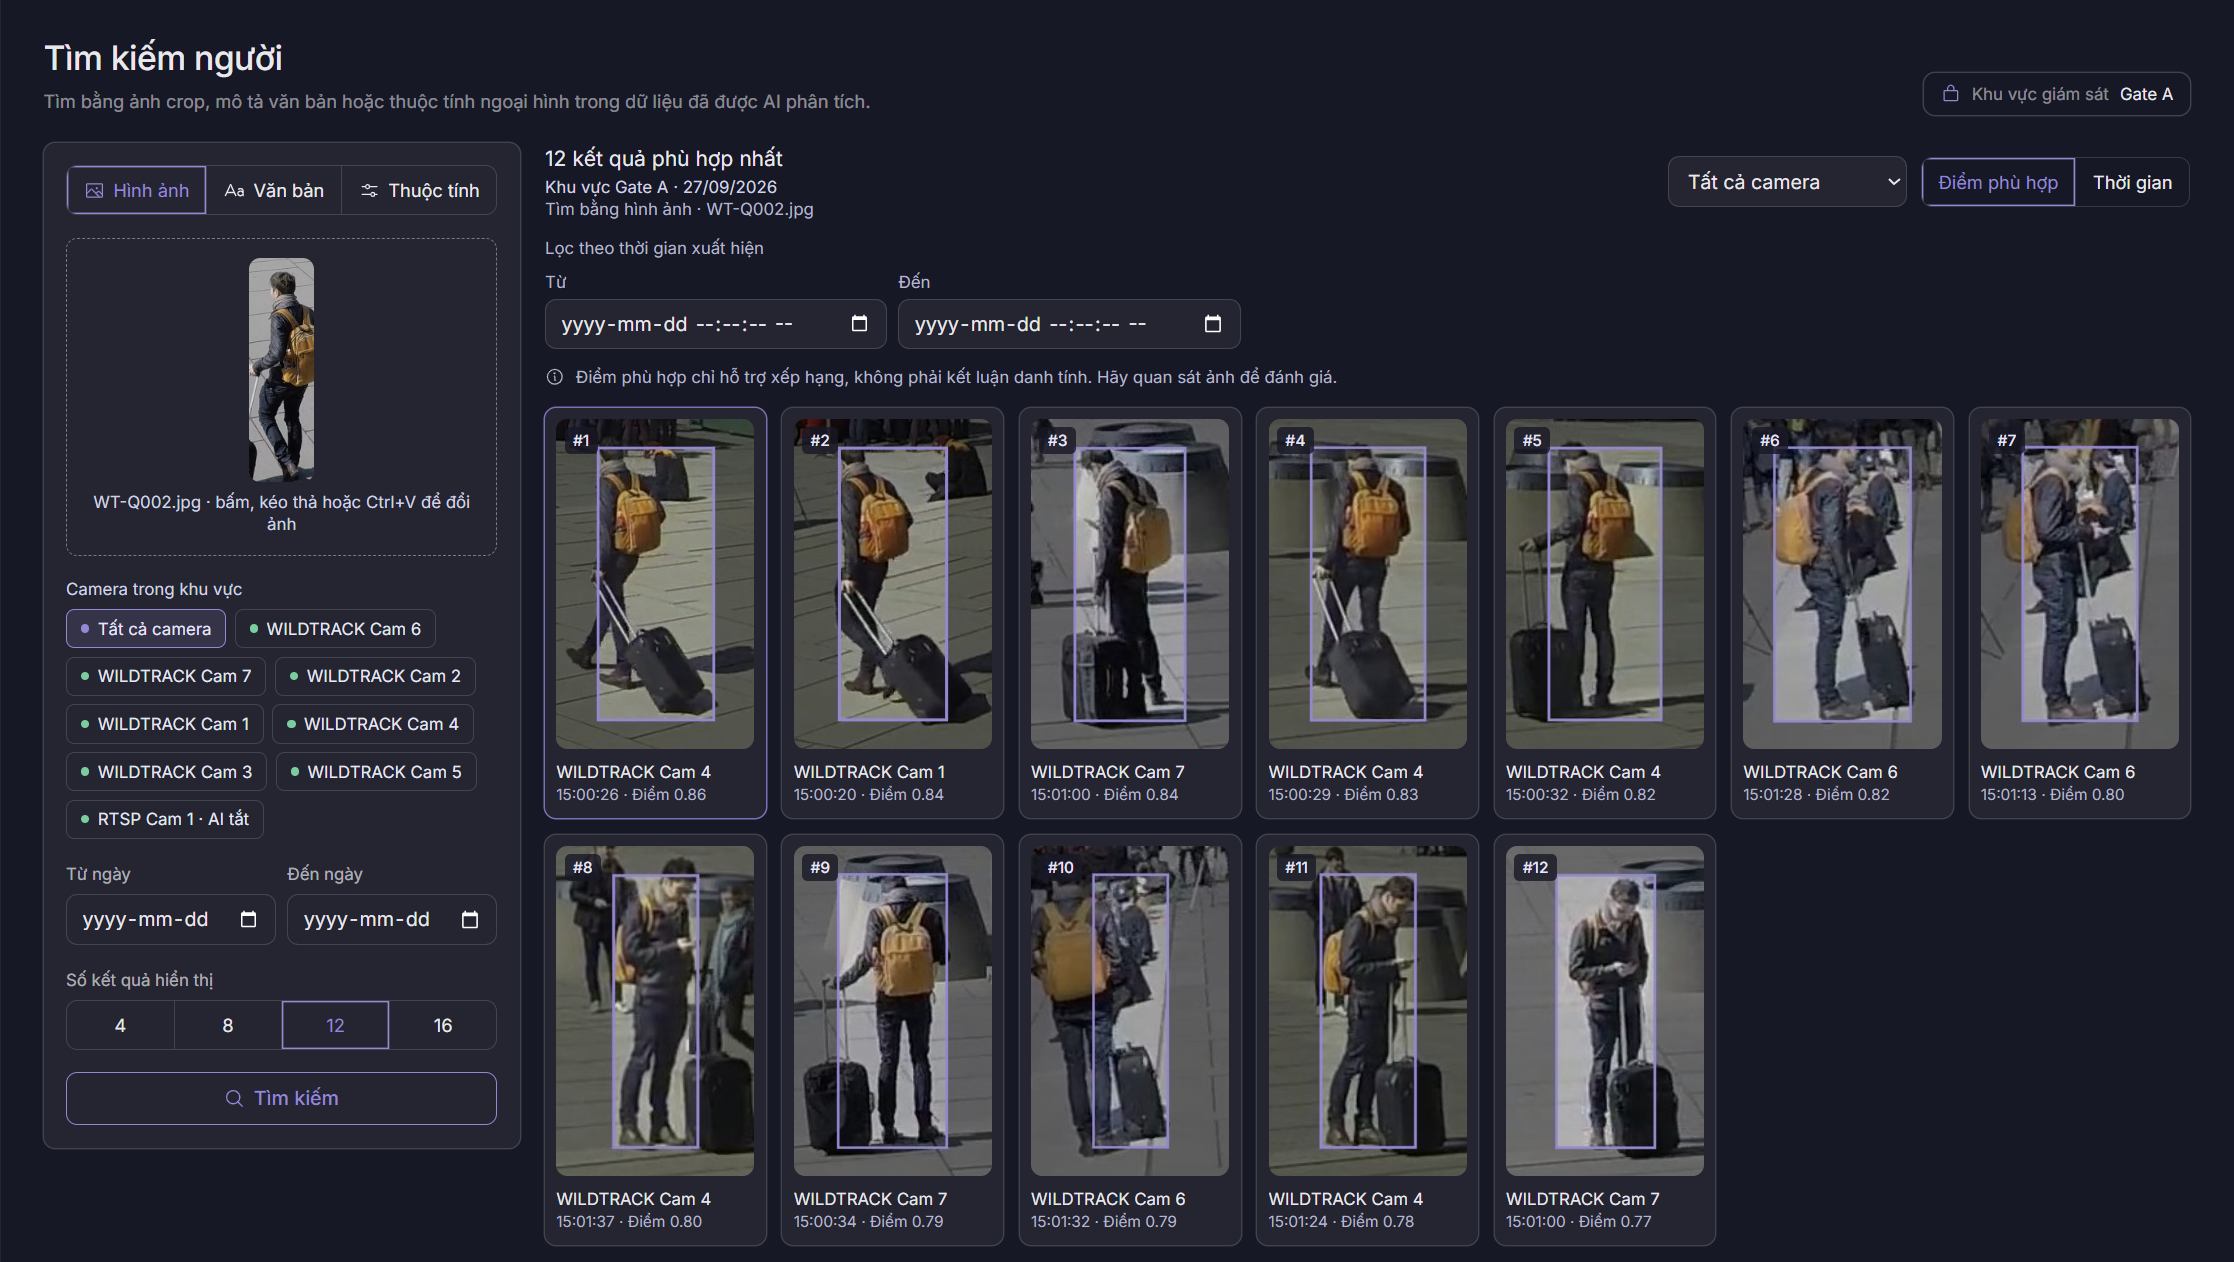
\includegraphics[width=\textwidth]{H10a-tim-kiem-anh-cat.png}
\caption{Màn hình tìm kiếm người bằng ảnh}
\label{fig:ui-search-image}
\end{figure}

\begin{figure}[!htbp]
\centering
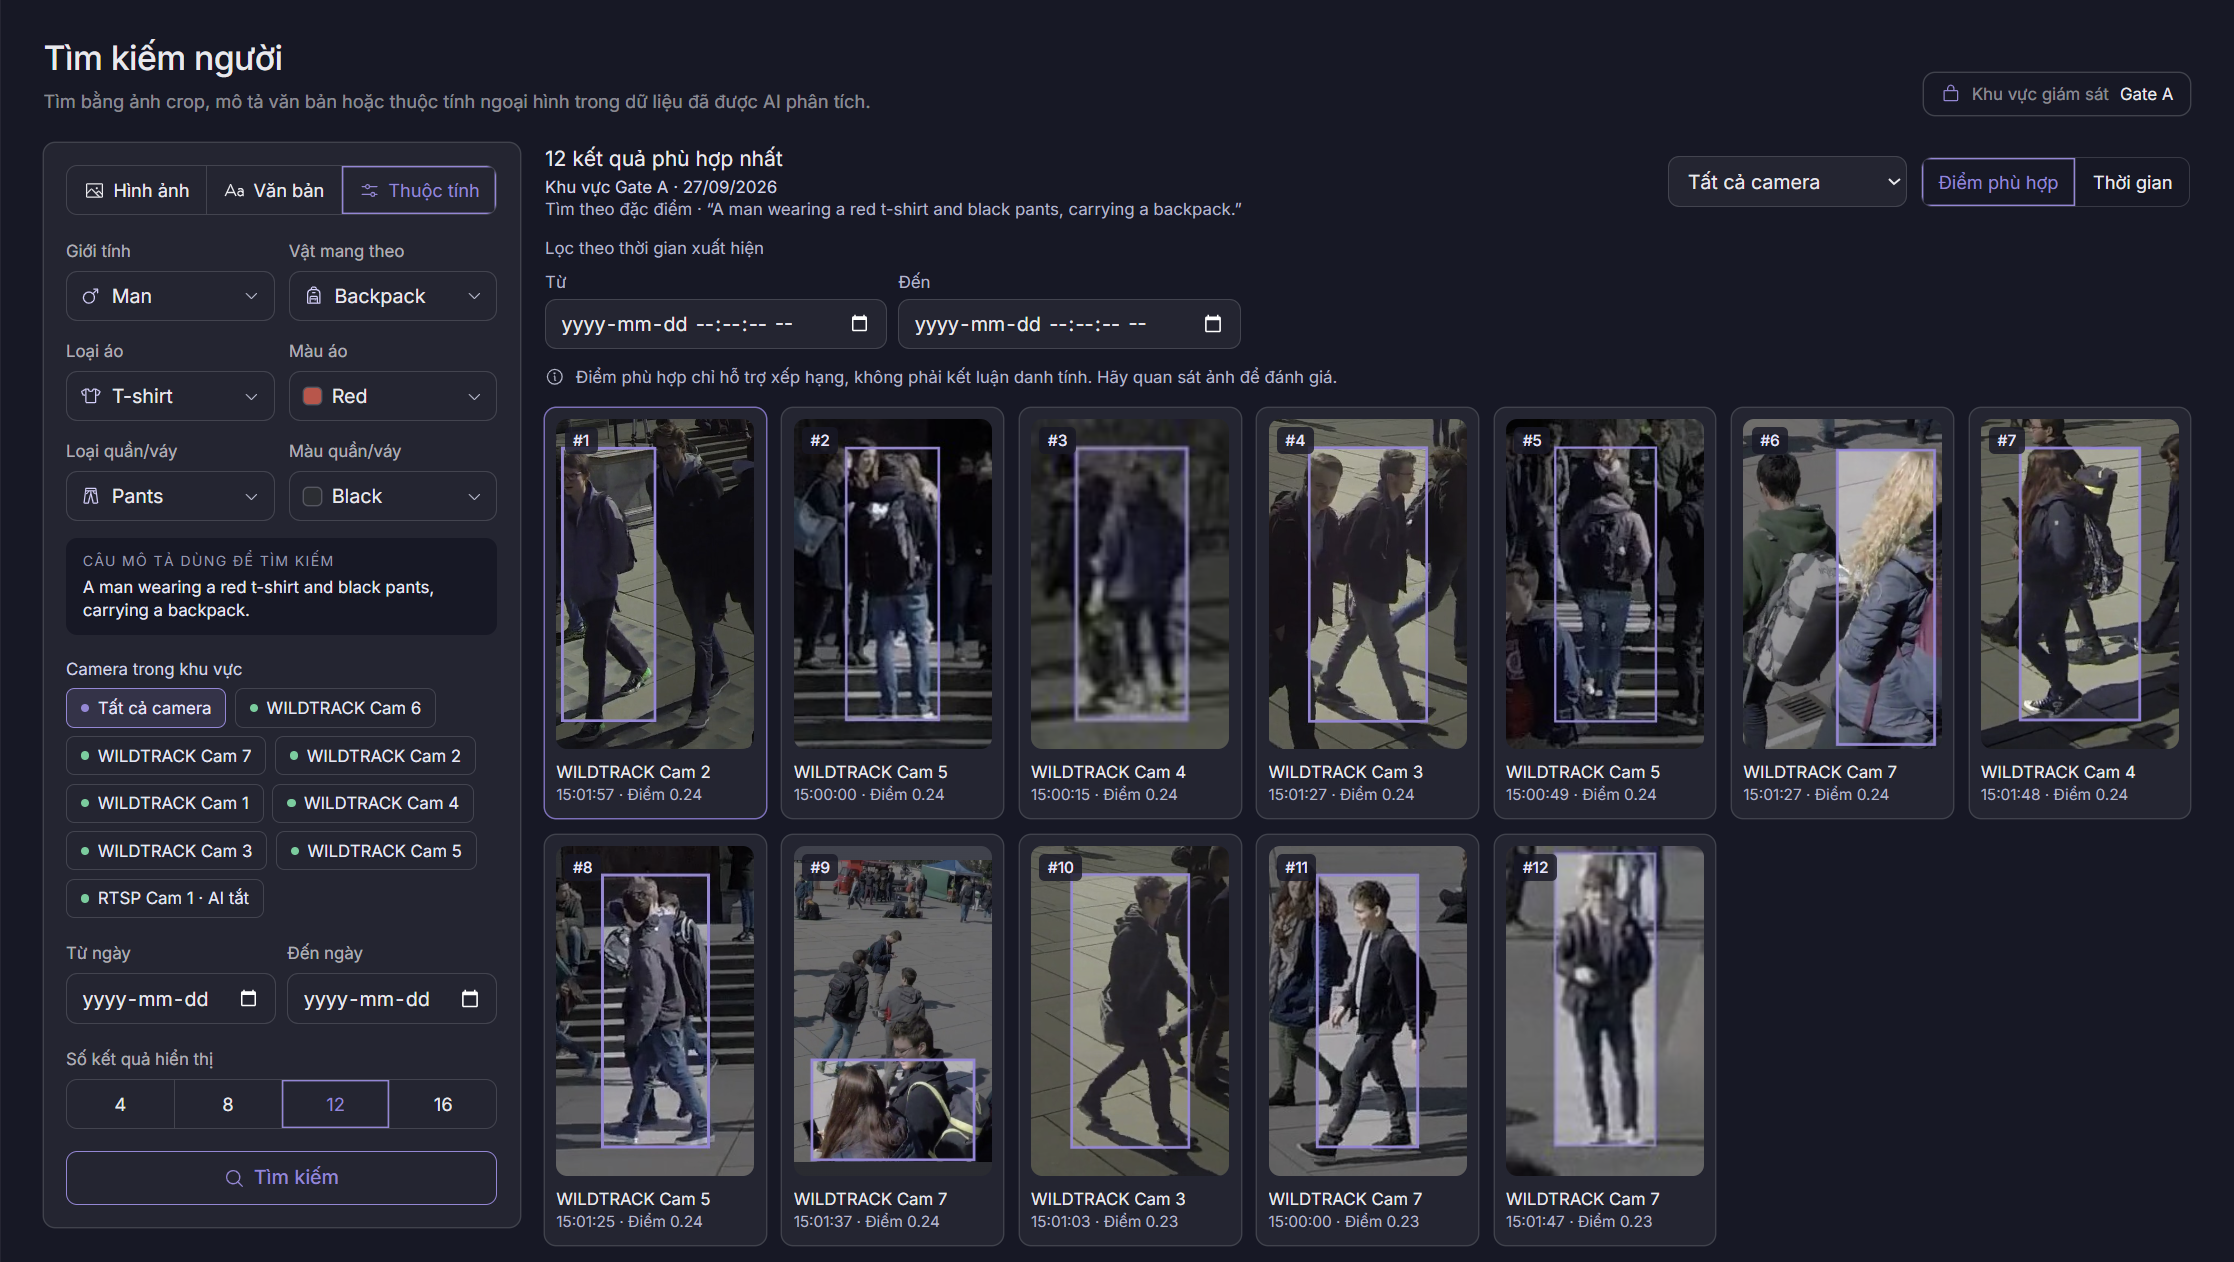
\includegraphics[width=\textwidth]{H10b-tim-kiem-thuoc-tinh-cat.png}
\caption{Màn hình tìm kiếm người theo thuộc tính}
\label{fig:ui-search-attr}
\end{figure}

\begin{figure}[!htbp]
\centering
\begin{subfigure}[b]{0.61\textwidth}
    \centering
    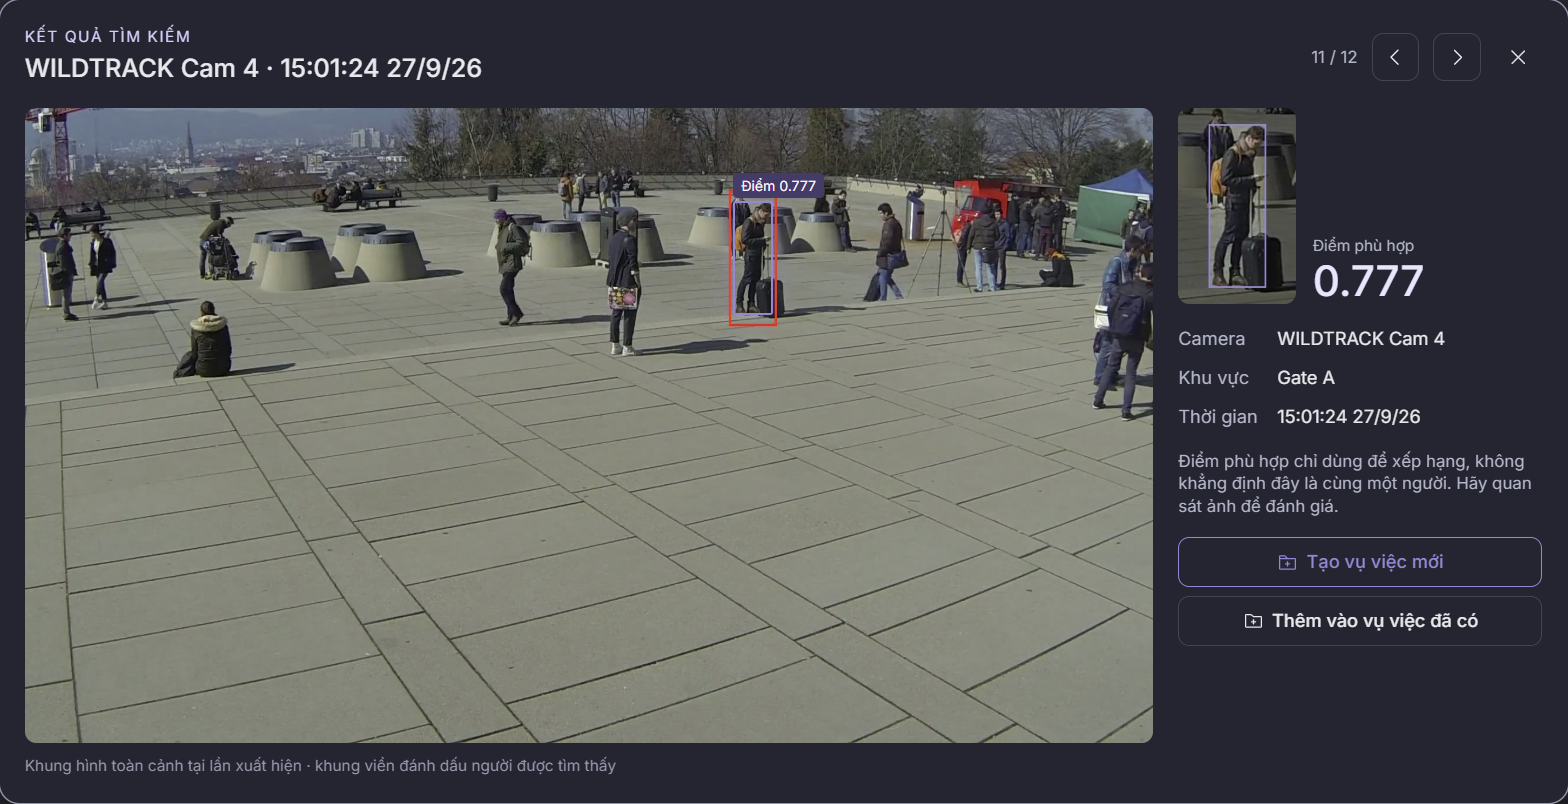
\includegraphics[width=\linewidth]{H10c-chi-tiet-ket-qua-cat.png}
    \caption{Chi tiết một kết quả}
    \label{fig:ui-result}
\end{subfigure}\hfill
\begin{subfigure}[b]{0.36\textwidth}
    \centering
    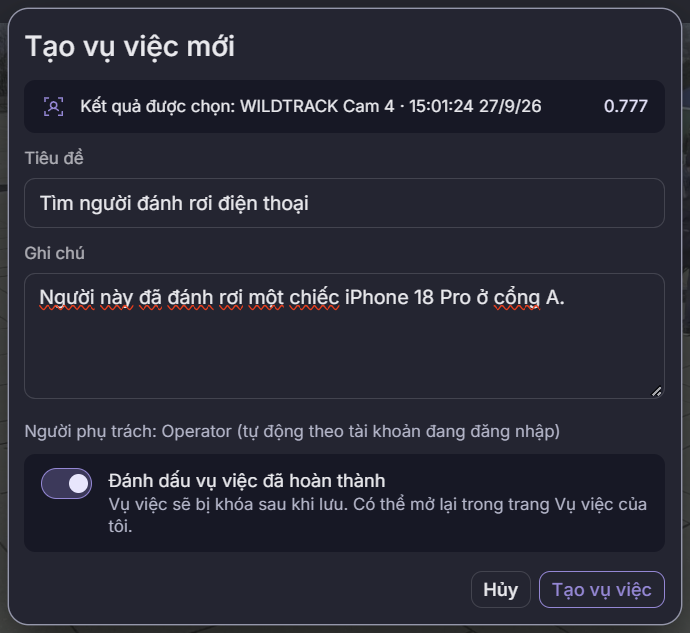
\includegraphics[width=\linewidth]{H10d-tao-vu-viec-cat.png}
    \caption{Tạo vụ việc mới từ kết quả}
    \label{fig:ui-create-case}
\end{subfigure}
\caption{Hộp thoại chi tiết kết quả và hộp thoại tạo vụ việc}
\label{fig:ui-result-case}
\end{figure}

\begin{figure}[!htbp]
\centering
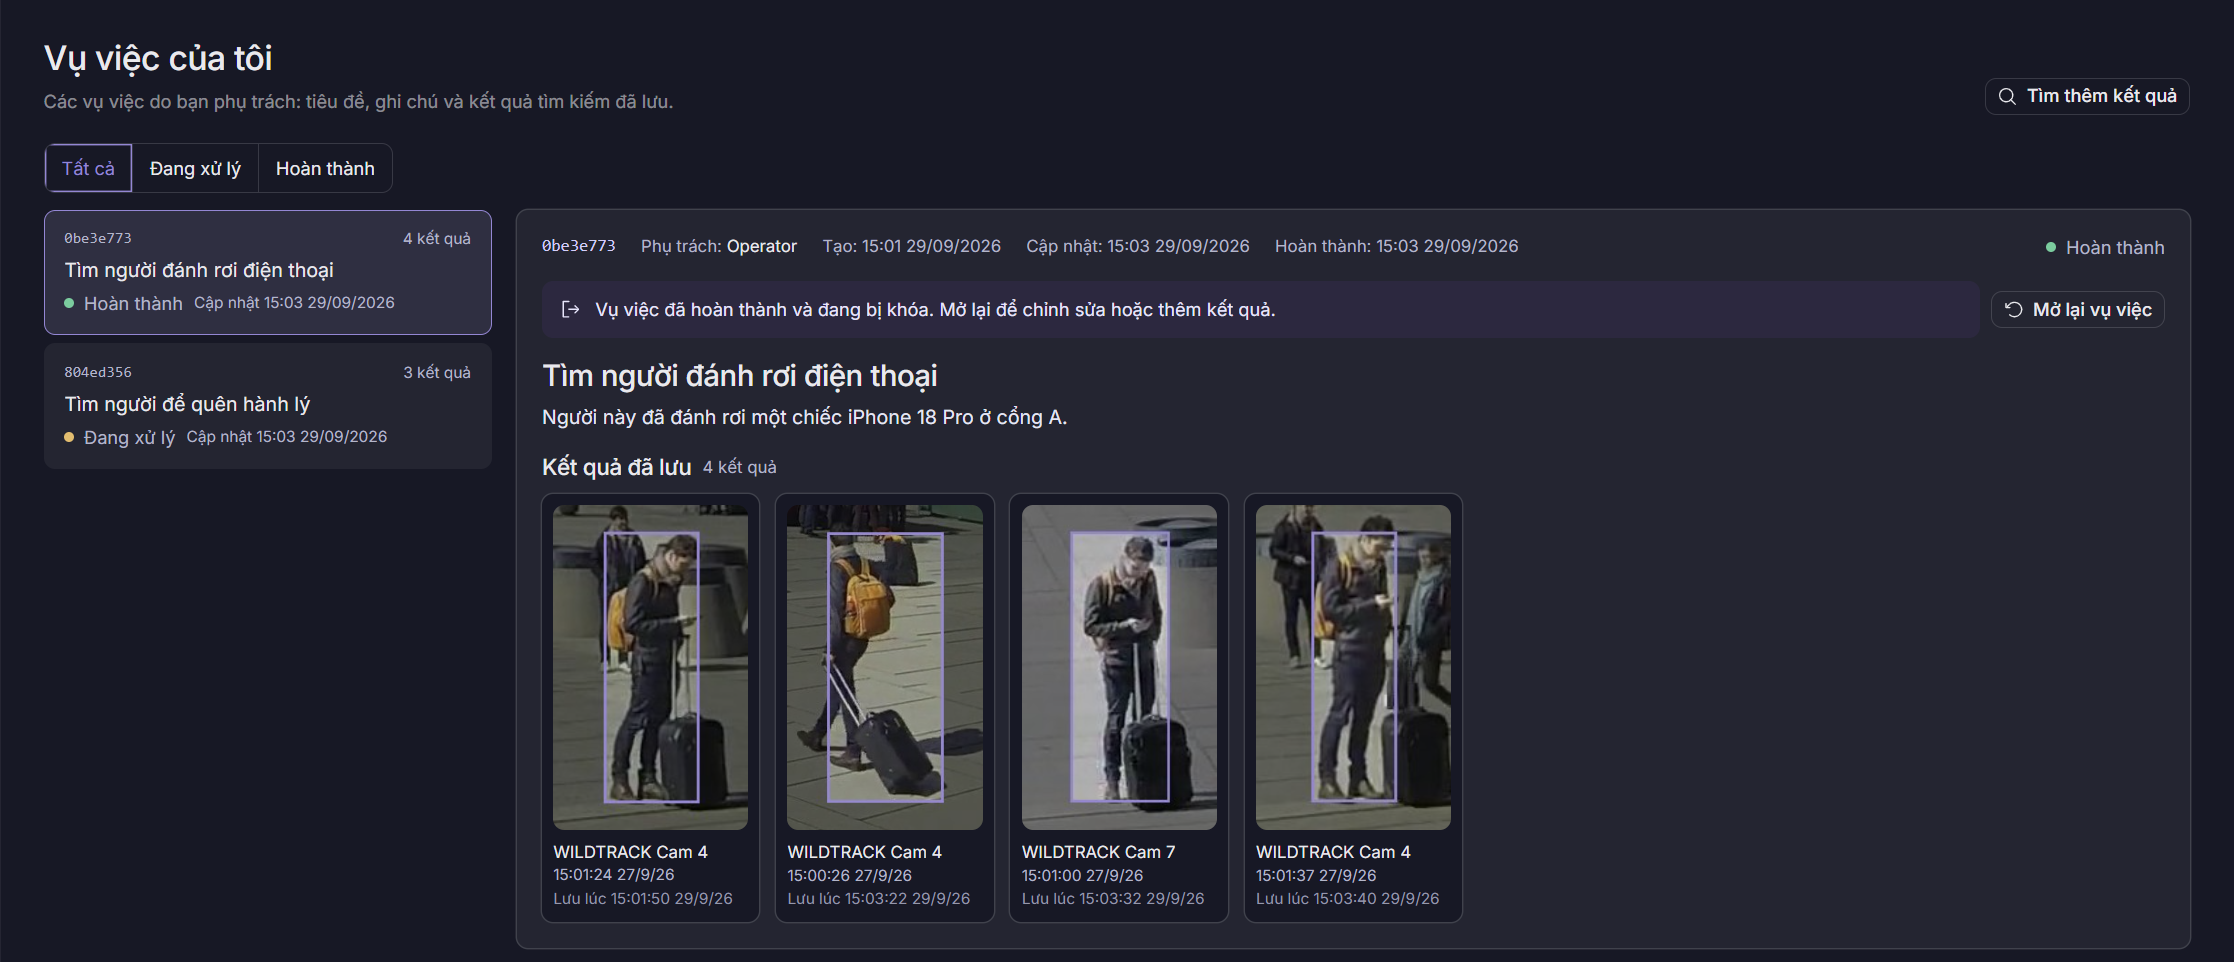
\includegraphics[width=\textwidth]{H10e-vu-viec-cua-toi-cat.png}
\caption{Màn hình quản lý vụ việc của Giám sát viên}
\label{fig:ui-cases}
\end{figure}

\paragraph{Quản lý.} Màn hình \emph{Tổng quan} (Hình~\ref{fig:ui-overview}) hiển thị số vụ việc theo trạng thái, số kết quả đã lưu và danh sách vụ việc gần đây; chọn một vụ việc mở màn hình \emph{Hồ sơ vụ việc}, có cùng bố cục như Hình~\ref{fig:ui-cases} nhưng ở chế độ chỉ đọc.

\begin{figure}[!htbp]
\centering
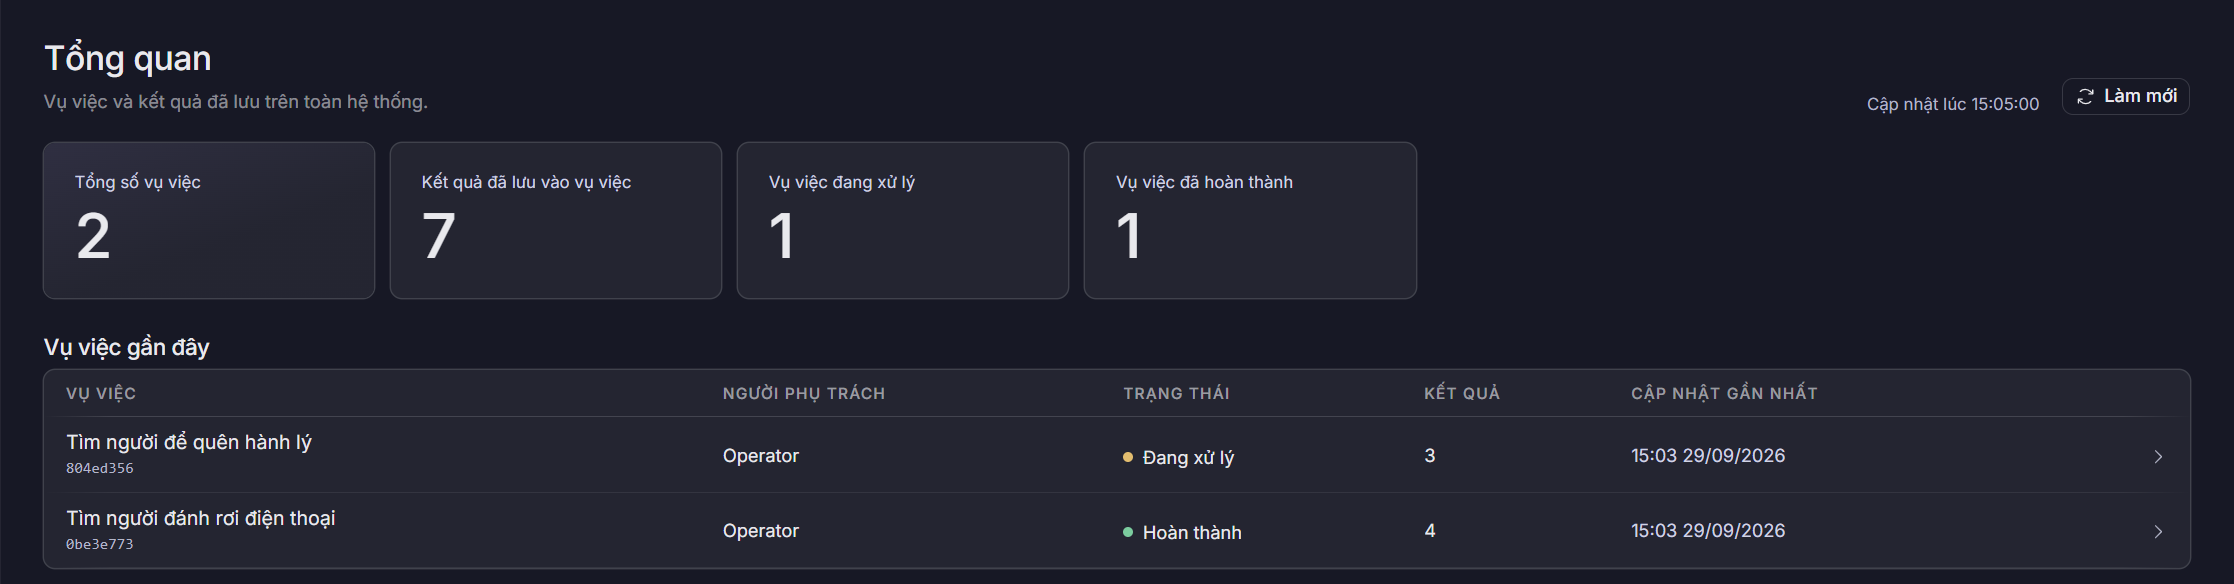
\includegraphics[width=\textwidth]{H10f-tong-quan-cat.png}
\caption{Màn hình tổng quan của Quản lý}
\label{fig:ui-overview}
\end{figure}

\paragraph{Quản trị viên.} Màn hình \emph{Camera} (Hình~\ref{fig:ui-cameras}) liệt kê các camera theo khu vực cùng trạng thái kết nối, trong đó camera chỉ xử lý tệp video được ghi là \emph{Video tải lên}, trạng thái xử lý AI và các thao tác kiểm tra kết nối, sửa, loại khỏi vận hành. Màn hình \emph{Mô hình AI} (Hình~\ref{fig:ui-models}) cho chọn Detector và Tracker; mô hình không đủ điều kiện được đánh dấu \emph{Không khả dụng}, còn bộ mã hóa được hiển thị là thành phần cố định (Mục~\ref{sec:6.2.1}). Màn hình \emph{Xử lý video} (Hình~\ref{fig:ui-video}) dùng để tải video lên cho một camera với chế độ lấy mẫu định sẵn và theo dõi tiến độ từng công việc theo số khung hình và số track đã sẵn sàng. Hai màn hình giám sát là \emph{Trạng thái hệ thống} (Hình~\ref{fig:ui-status}, Mục~\ref{sec:6.4}) và \emph{Kiểm tra AI} (Hình~\ref{fig:ui-diagnostics}, Mục~\ref{sec:6.2.5}).

\begin{figure}[!htbp]
\centering
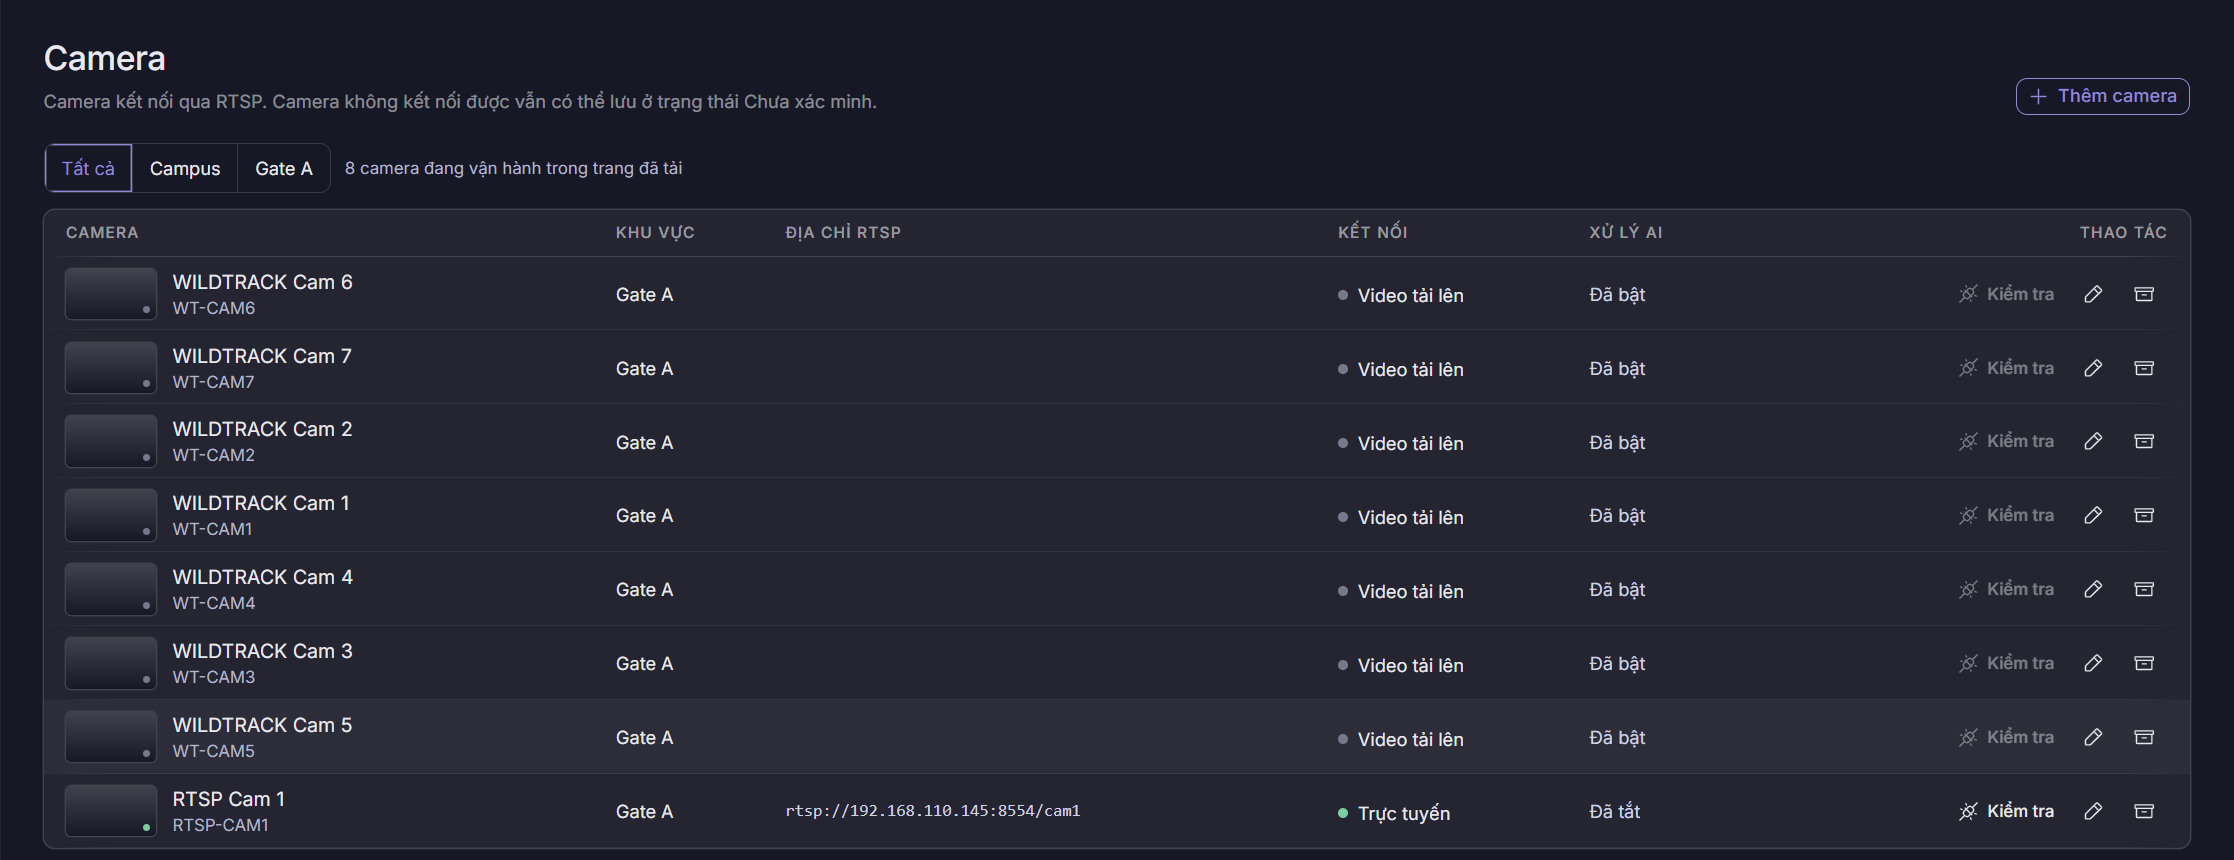
\includegraphics[width=\textwidth]{H10g-camera-cat.png}
\caption{Màn hình quản lý camera}
\label{fig:ui-cameras}
\end{figure}

\begin{figure}[!htbp]
\centering
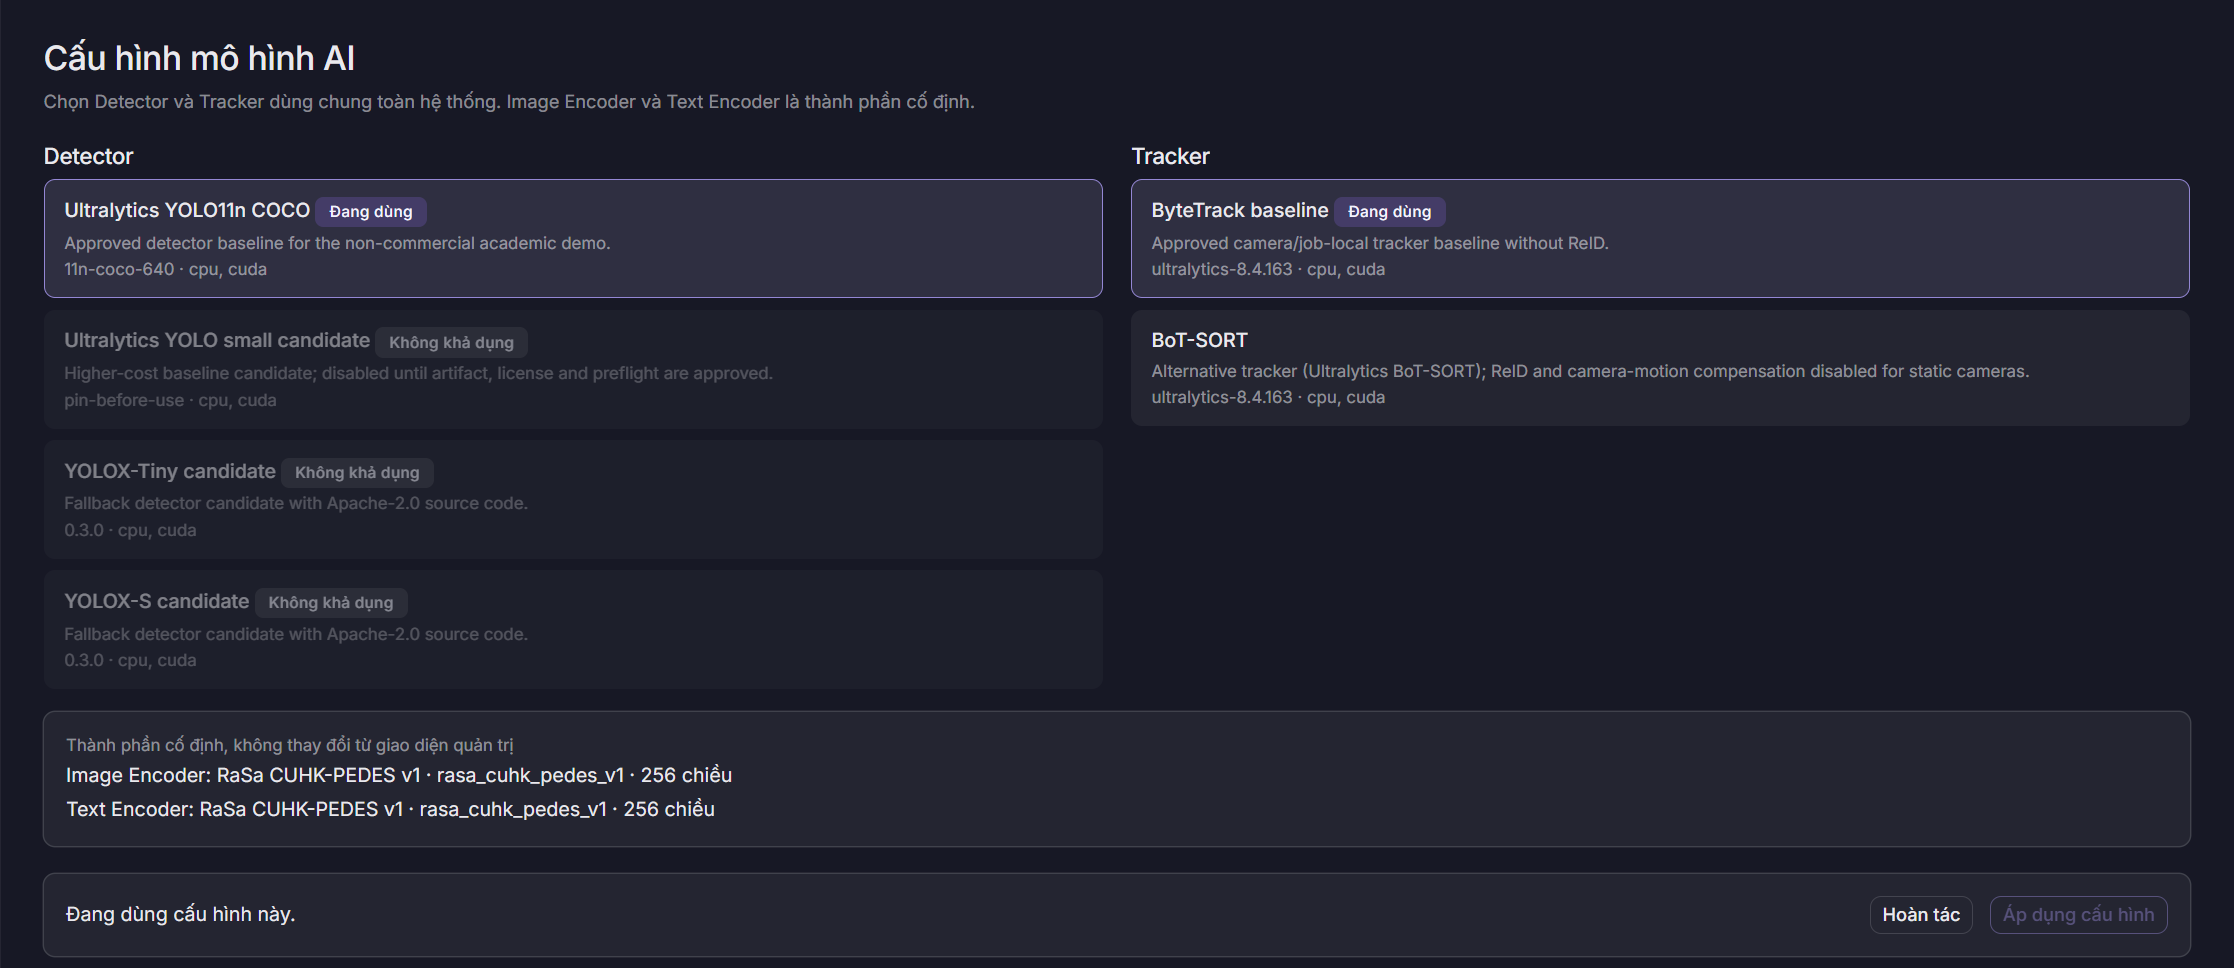
\includegraphics[width=\textwidth]{H10h-mo-hinh-ai-cat.png}
\caption{Màn hình cấu hình mô hình AI}
\label{fig:ui-models}
\end{figure}

\begin{figure}[!htbp]
\centering
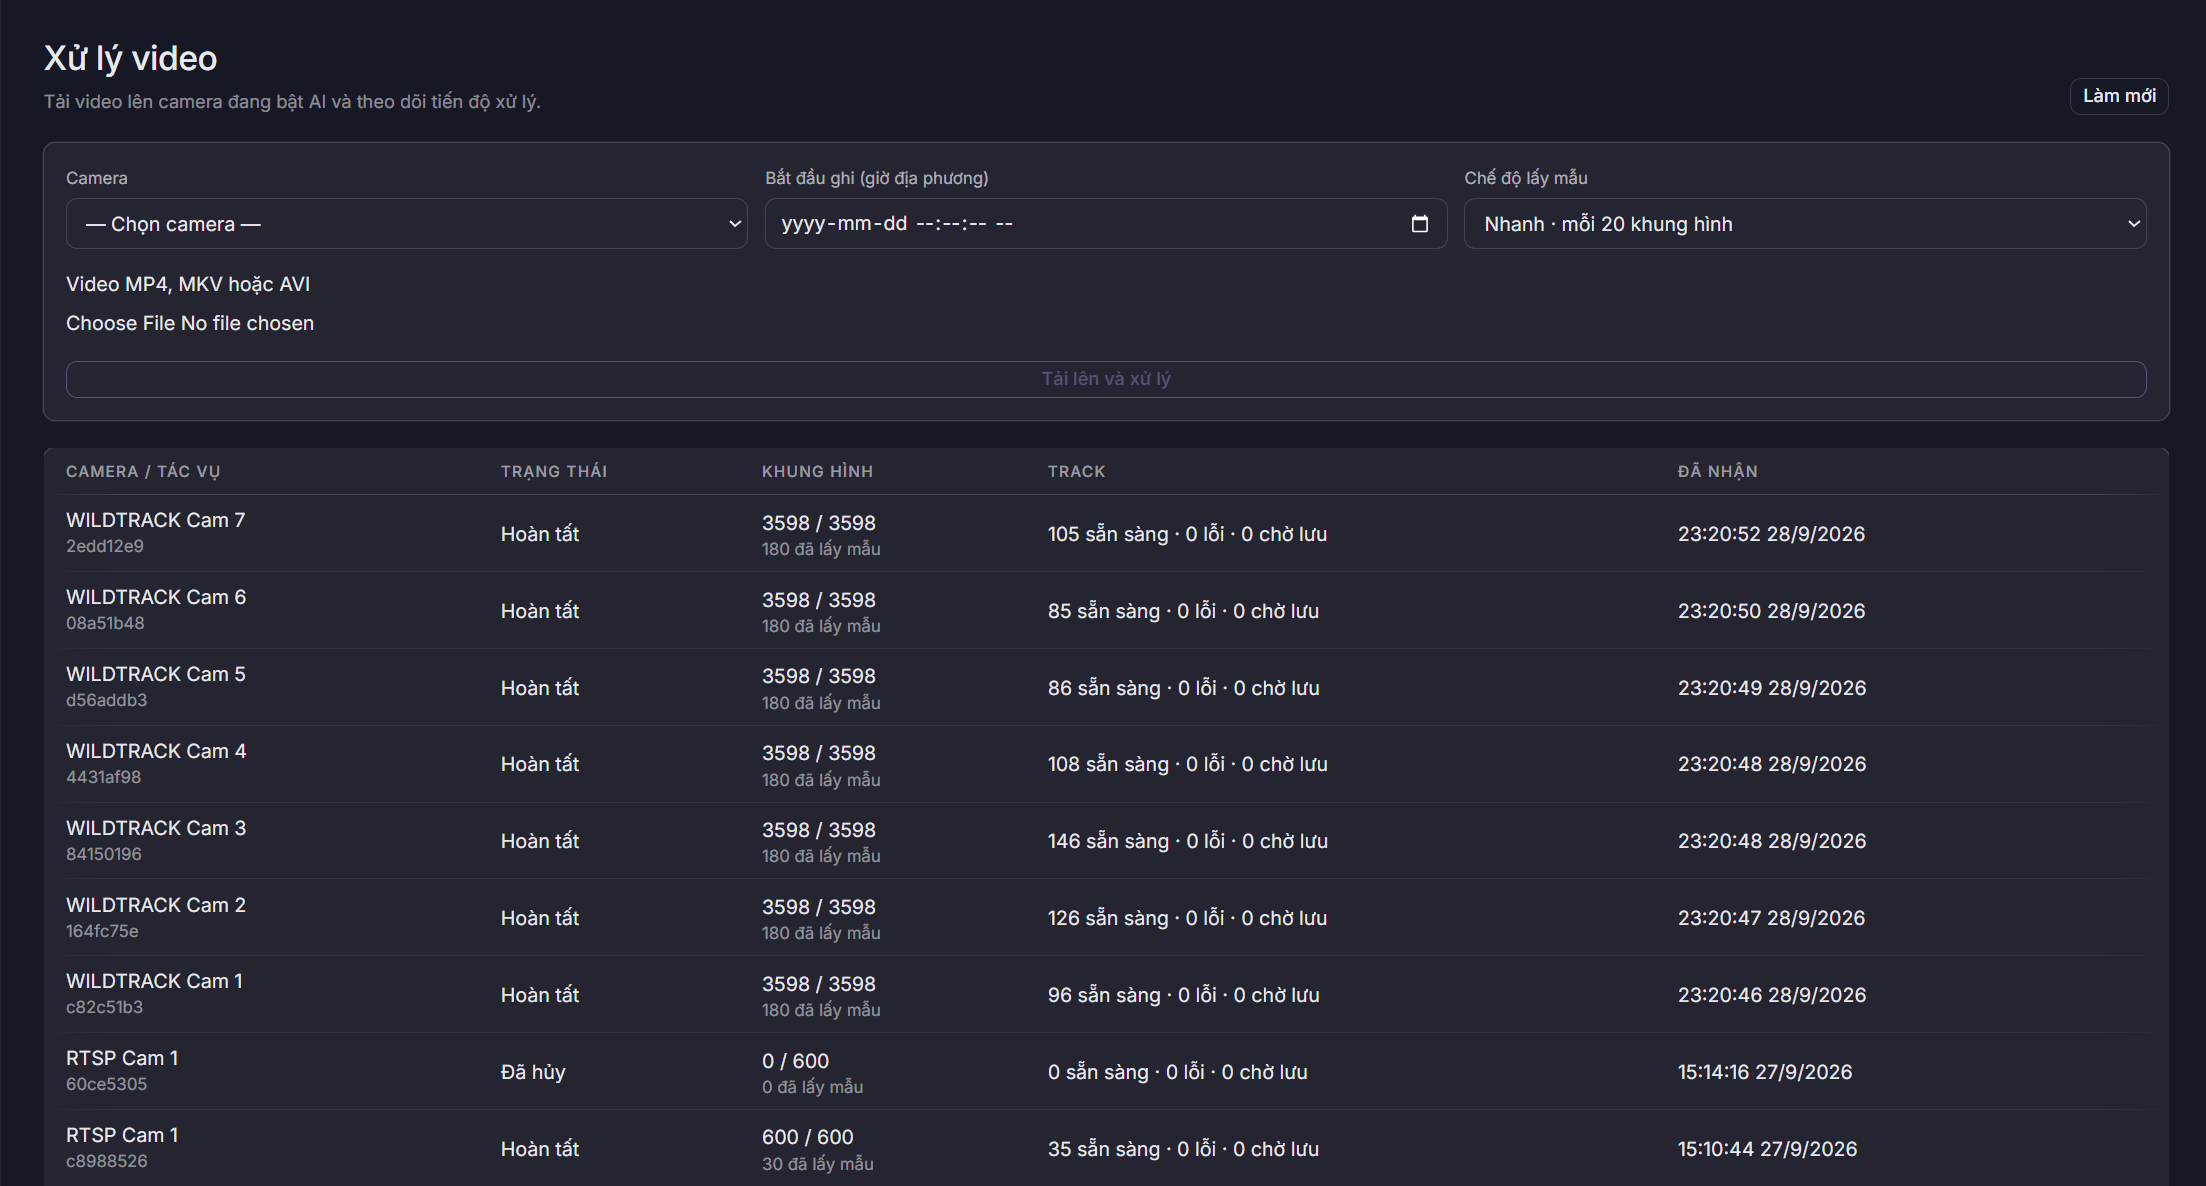
\includegraphics[width=\textwidth]{H10i-xu-ly-video-cat.png}
\caption{Màn hình xử lý video tải lên}
\label{fig:ui-video}
\end{figure}

\begin{figure}[!htbp]
\centering
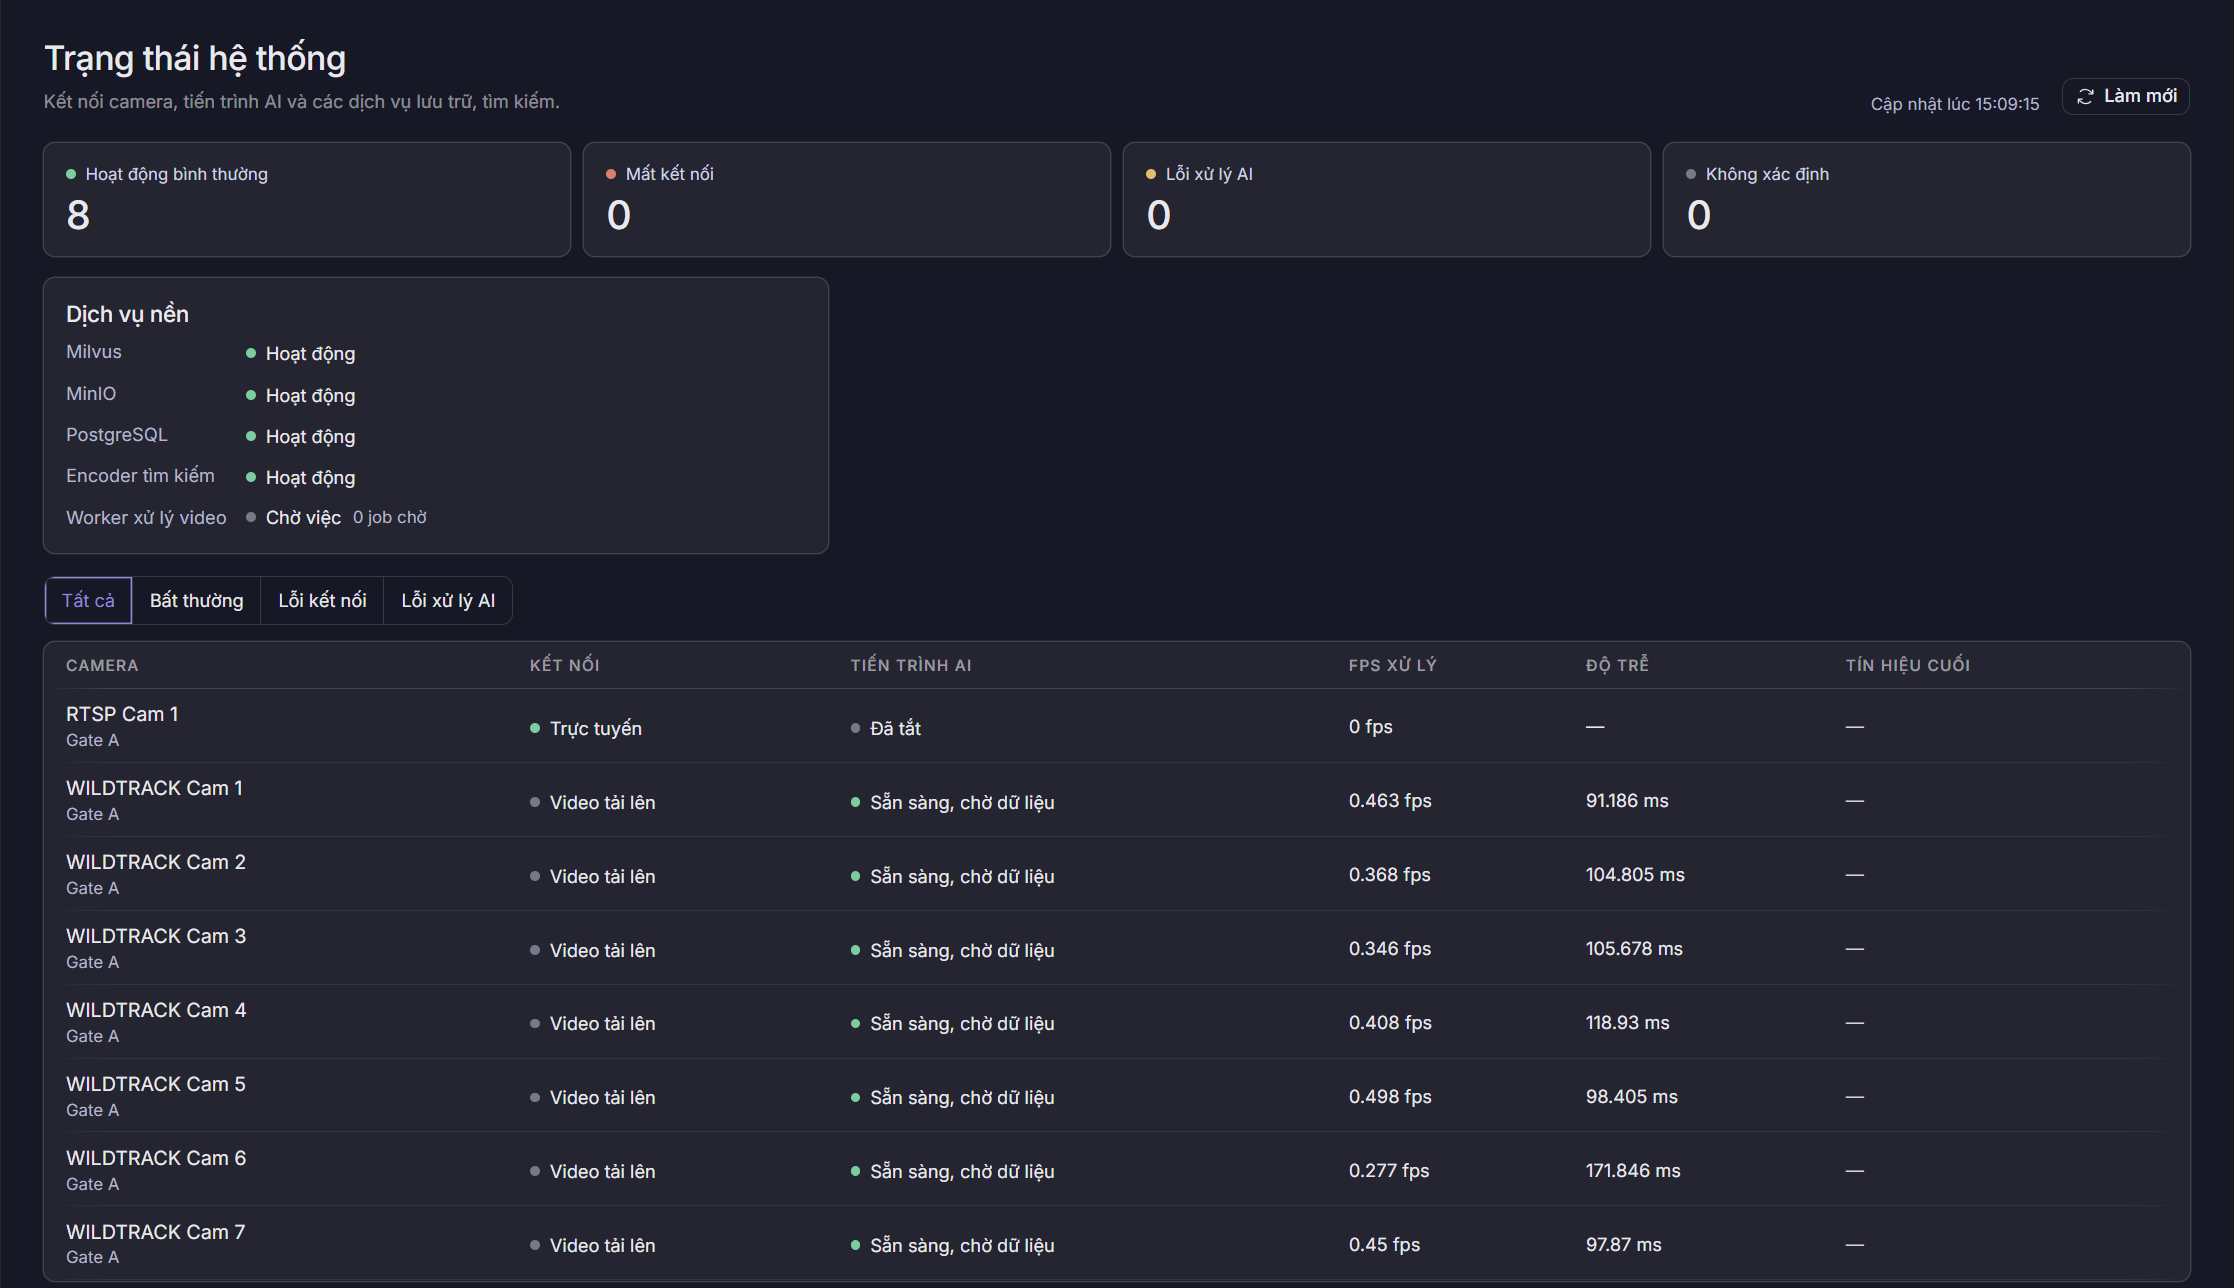
\includegraphics[width=\textwidth]{H10j-trang-thai-he-thong-cat.png}
\caption{Màn hình trạng thái hệ thống}
\label{fig:ui-status}
\end{figure}

\begin{figure}[!htbp]
\centering
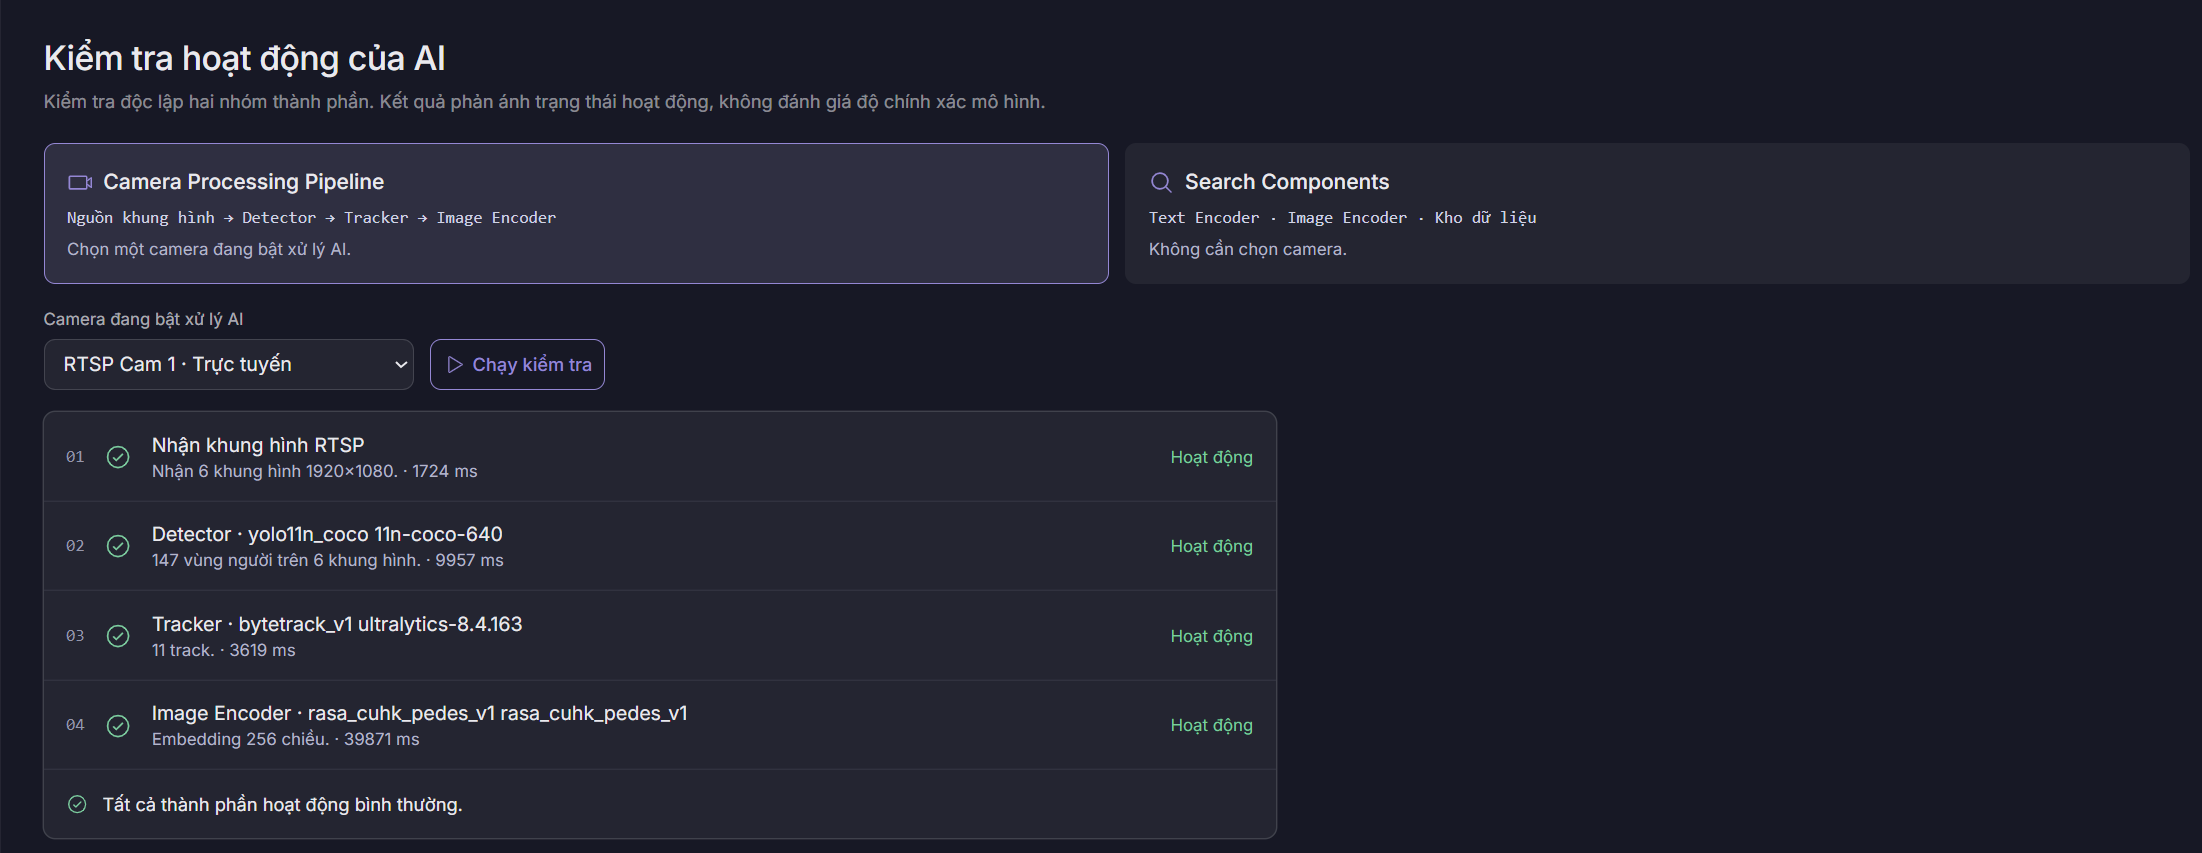
\includegraphics[width=\textwidth]{H10k-kiem-tra-ai-cat.png}
\caption{Màn hình kiểm tra hoạt động của AI}
\label{fig:ui-diagnostics}
\end{figure}

% !TEX root = ../../main.tex
% C6.4 — Giám sát vận hành (bản ngắn)
% Nội dung cần có: nhật ký JSON có mã yêu cầu xuyên API -> worker, che trường nhạy cảm, số đo, heartbeat, màn hình trạng thái.
\section{Giám sát vận hành}
\label{sec:6.4}

\nhap{Chưa viết.}


% !TEX root = ../../main.tex
% Chương 7 — xem mục C7 trong report/report_plan.md. Số liệu chỉ lấy từ files/report-data-guide.md mục 3 (quy tắc ở mục 1).
% Cấu trúc rút gọn 2026-09-29 (giới hạn 90 trang): 7.3 gộp vào 7.1; không vẽ sơ đồ triển khai H9 (H2 đã thể hiện các thành phần).
\chapter{Triển khai hệ thống}
\label{chapter:trienkhai}

\textit{Chương này trình bày môi trường và quy trình triển khai hệ thống, cùng dữ liệu thử nghiệm và cách giả lập hệ thống camera.}

% !TEX root = ../../main.tex
% C7.1 — Môi trường và quy trình triển khai (gộp 7.3 cũ). Số liệu: report-data-guide.md mục 2 (máy), mục 3 C7.3 (sao lưu/khôi phục, Hiện hành).
% Phiên bản dịch vụ: infra/compose.yaml (PostgreSQL 17.11, Milvus 2.6.24 + etcd 3.5.25, MinIO RELEASE.2024-12-18, MediaMTX 1.12.3).
% Thứ tự khởi động và làm nóng: files/demo-script.md mục 3. Khôi phục: remaining-work-plan R6, STO-19.
\section{Môi trường và quy trình triển khai}
\label{sec:7.1}
\label{sec:7.3}

\paragraph{Môi trường.} Toàn bộ hệ thống được triển khai trên một máy tính xách tay dùng bộ xử lý Intel Core i5-11300H (4 nhân, 8 luồng, 3,1~GHz), 16~GB bộ nhớ, không có card đồ họa rời, chạy Windows 11. Các dịch vụ hạ tầng chạy trong Docker Compose, gồm PostgreSQL 17, Milvus 2.6 ở chế độ Standalone cùng etcd, MinIO dùng chung cho Milvus và cho khung hình của ứng dụng, và MediaMTX để phát các luồng camera giả lập. Máy chủ ứng dụng Flask và tiến trình xử lý nền chạy trực tiếp trên máy; ứng dụng web React được build một lần và các tệp tĩnh của nó do máy chủ ứng dụng phục vụ trên cùng origin, nên khi trình diễn không cần máy chủ phát triển, proxy hay cấu hình cross-origin. Máy ảo WSL~2 phía sau Docker Desktop được giới hạn 3~GB bộ nhớ, vì mặc định nó có thể chiếm tới một nửa bộ nhớ máy trong khi các container chỉ cần khoảng 0,4~GiB (Mục~\ref{sec:8.7}). Cấu hình AI gồm YOLO11n với ngưỡng tin cậy 0,1, ByteTrack, bộ mã hóa RaSa và khoảng lấy mẫu $N = 20$, tất cả chạy trên CPU.

\paragraph{Quy trình khởi động.} Các thành phần khởi động theo thứ tự: hạ tầng, luồng camera, máy chủ ứng dụng (đồng thời phục vụ ứng dụng web), tiến trình nền. Một lượt tìm kiếm làm nóng nạp bộ mã hóa truy vấn trước khi sử dụng (Mục~\ref{sec:8.7}).

\paragraph{Sao lưu và khôi phục.} Bản sao lưu dữ liệu trình diễn của ba kho có dung lượng khoảng 510~MB, gồm 1.525 tệp. Quy trình khôi phục được diễn tập với 1.555 track, trong đó 10 khung hình bị xóa có chủ đích: việc khôi phục hoàn tất trong 28,8 giây (PostgreSQL 1,8 giây; khung hình 6,2 giây, tải lại đủ 10/10 tệp; dựng lại vector trong Milvus 8,8 giây; đối soát ba kho 12 giây). Lần diễn tập đầu, ghi vector từng cái một, mất 1.485 giây và có một vector quá thời gian, dẫn tới việc chuyển sang ghi theo lô. Sau mỗi lần trình diễn thử, dữ liệu được đặt lại trong khoảng 70 giây.

% !TEX root = ../../main.tex
% C7.2 — Dữ liệu thử nghiệm và camera giả lập. Số liệu: report-data-guide.md mục 2 (dữ liệu demo 1.488 / 1.523 track) và mục 3 C7.2 (Hiện hành, R6).
% Không lấy số từ database đang chạy. WILDTRACK: chavdarova2018wildtrack (7 camera, 1920x1080, ~60 fps).
\section{Dữ liệu thử nghiệm và camera giả lập}
\label{sec:7.2}

\paragraph{Bộ dữ liệu.} Đề tài sử dụng bộ dữ liệu WILDTRACK~\cite{chavdarova2018wildtrack}, gồm video của bảy camera tĩnh độ phân giải 1920$\times$1080 cùng quan sát một khu vực đông người đi bộ ngoài trời, với vùng nhìn chồng lấn nhau, kèm nhãn vị trí người trên một tập khung hình. Mỗi video được xem là một camera, và cả bảy camera được gán vào cùng một khu vực giám sát.

\paragraph{Camera giả lập.} Bảy video được phát thành bảy luồng RTSP qua MediaMTX như Mục~\ref{sec:3.7.3}. Tuy nhiên, trên máy triển khai, quá trình phân tích chậm hơn thời gian thực khoảng bảy lần, nên máy phát luồng bỏ bớt khung hình và phần lớn nội dung của luồng không được phân tích. Vì vậy, luồng RTSP được dùng để trình diễn và kiểm chứng việc tiếp nhận camera (Mục~\ref{sec:8.6}), còn dữ liệu trình diễn được lập chỉ mục từ chính các tệp video qua chức năng tải video lên, đi qua cùng quy trình xử lý.

\paragraph{Chuẩn bị dữ liệu trình diễn.} Việc lập chỉ mục được thực hiện bằng một công cụ gọi API của hệ thống như Quản trị viên: công cụ cắt đoạn video cần xử lý, tải lên cho từng camera với cùng một mốc thời gian gốc cho cả bảy camera, rồi theo dõi tới khi công việc kết thúc. Dữ liệu trình diễn phủ 120 giây đầu của mỗi video: đoạn 0-60 giây tạo 736 track, đoạn 60-120 giây được xử lý bằng 7 công việc trong 55 phút, tạo thêm 752 track, không có lỗi. Tổng cộng có 1.488 track ở trạng thái sẵn sàng, phân bố như Bảng~\ref{tab:demo-tracks}. Cùng với 35 track từ một phiên xử lý luồng RTSP, dữ liệu trình diễn có 1.523 track và một vụ việc mẫu gồm 3 kết quả.

\begin{table}[H]
\centering
\caption{Số track của dữ liệu trình diễn theo camera (120 giây đầu mỗi video)}
\label{tab:demo-tracks}
\begin{tabularx}{\textwidth}{|L|c|c|c|c|c|c|c|c|}
\hline
\textbf{Camera} & C1 & C2 & C3 & C4 & C5 & C6 & C7 & \textbf{Tổng} \\
\hline
\textbf{Số track} & 208 & 254 & 308 & 188 & 182 & 159 & 189 & 1.488 \\
\hline
\end{tabularx}
\end{table}


% !TEX root = ../../main.tex
% Chương 8 — xem mục C8 trong report/report_plan.md. Số liệu CHỈ lấy từ files/report-data-guide.md mục 3, theo cột "Trạng thái":
% Hiện hành dùng trực tiếp; Cũ kèm câu nêu điều kiện đo; Chưa đo thì viết phương pháp, ghi "chưa đo". Không tự đo, không lấy số từ database đang chạy.
% Cấu trúc rút gọn 2026-09-29: 8.1 = C8.1–C8.3; 8.2 = C8.4; 8.3 = C8.5–C8.7 (nhãn cũ giữ nguyên để không gãy tham chiếu).
\chapter{Kiểm thử và đánh giá hệ thống}
\label{chapter:kiemthu}

\textit{Chương này trình bày kết quả kiểm thử phần mềm, đánh giá chất lượng tìm kiếm, và các số đo về tốc độ xử lý, luồng RTSP và tài nguyên của hệ thống.}

% !TEX root = ../../main.tex
% C8.1–C8.3 — Kiểm thử phần mềm. Số liệu: report-data-guide.md mục 3, dòng C8.1–C8.3 (đều Hiện hành): unit 740 (2026-10-05), integration (R3),
% E2E (R3), giao diện (R5), diễn tập demo (R7), phân quyền/bảo mật (tests/unit/test_hardening.py, test_cases_api.py; R2).
% Mô tả E2E phân quyền: ai_worker_implementation_plan.md AIW-25 (chỉ mô tả, không có số).
\section{Kiểm thử phần mềm}
\label{sec:8.1}
\label{sec:8.2}
\label{sec:8.3}

Hệ thống được kiểm thử ở năm mức, từ từng hàm tới toàn bộ kịch bản trình diễn (Bảng~\ref{tab:test-levels}), bằng pytest phía máy chủ và Playwright tự động trên Edge cho giao diện. Kiểm thử tích hợp và đầu cuối từ chối chạy nếu tên cơ sở dữ liệu không mang hậu tố kiểm thử, nên dữ liệu trình diễn không bị ghi nhầm.

\begin{table}[H]
\centering
\caption{Kết quả kiểm thử theo từng mức}
\label{tab:test-levels}
\begin{tabularx}{\textwidth}{|>{\raggedright\arraybackslash}p{2.9cm}|L|>{\raggedright\arraybackslash}p{4.4cm}|}
\hline
\textbf{Mức} & \textbf{Phạm vi} & \textbf{Kết quả} \\
\hline
Đơn vị (unit) & Từng thành phần của máy chủ và tiến trình xử lý nền, gồm cả kiểm thử hợp đồng API, bảo mật và chèn lỗi & 740 đạt \\
\hline
Tích hợp & Với PostgreSQL, Milvus, MinIO và MediaMTX thật: kết nối các kho; các dịch vụ nghiệp vụ; bộ chuyển đổi lưu trữ; di chuyển và lược đồ cơ sở dữ liệu; luồng RTSP & 37 đạt, 1 bỏ qua (chèn lỗi cần tắt hẳn một dịch vụ) \\
\hline
Đầu cuối (E2E) & Toàn bộ luồng qua API thật với các mô hình thật: tải video, lập chỉ mục, tìm kiếm, lưu vụ việc, xem với vai trò Quản lý & 2 đạt; luồng AI với đoạn video 10 giây mất 217 giây (nạp mô hình 44 giây, xử lý 154 giây, lần tìm bằng văn bản đầu tiên 16 giây) \\
\hline
Giao diện & 20 màn hình ở ba độ rộng 390, 768 và 1440 điểm ảnh & Không phần tử bị tràn, không lỗi trình duyệt hay lỗi HTTP; 3 lỗi được phát hiện và đã sửa \\
\hline
Kịch bản trình diễn & Các bước của ba vai trò, từ thêm camera RTSP tới xem hồ sơ vụ việc, chạy tự động & 2 lần liên tiếp đạt 15/15 bước, 85-88 giây thao tác \\
\hline
\end{tabularx}
\end{table}

Ba lỗi giao diện gồm: không chọn được mô hình trên màn hình mô hình AI, lần tìm đầu hết thời gian chờ trước khi nạp xong bộ mã hóa, và màn hình camera hiển thị sai trạng thái xử lý AI.

\paragraph{Kiểm thử phân quyền và bảo mật.} Các kiểm thử này nằm trong nhóm kiểm thử đơn vị và bao phủ ma trận phân quyền ở Mục~\ref{sec:4.6}:
\begin{itemize}
    \item Mọi API phải khai báo quy tắc truy cập; một kiểm thử gọi từng API với từng vai trò và khi chưa đăng nhập, kiểm tra chỉ vai trò được phép mới qua được.
    \item Giám sát viên mở vụ việc của người khác nhận mã 404; Quản lý chỉ đọc được vụ việc; lần xuất hiện ngoài khu vực và ảnh thuộc vụ việc khác đều bị chặn. Kiểm thử đầu cuối xác nhận thêm rằng Giám sát viên ở khu vực khác không tìm thấy và không mở được khung hình của lần xuất hiện, còn Quản lý không gọi được chức năng tìm kiếm.
    \item Mọi thao tác ghi đều đòi mã chống giả mạo. Đăng nhập bị giới hạn tần suất theo địa chỉ IP và tên đăng nhập, còn tìm kiếm theo tài khoản. Các tiêu đề bảo mật có mặt ở cả phản hồi thành công lẫn phản hồi lỗi, và chỉ các nguồn được cấu hình mới được gọi API kèm cookie.
\end{itemize}

% !TEX root = ../../main.tex
% C8.4 — Đánh giá chất lượng tìm kiếm. Số liệu: report-data-guide.md mục 3 dòng C8.4.
% Lần 1 = CŨ (ngưỡng Detector 0,25; gallery 1.552 track; 6 truy vấn; var/evaluation/wildtrack-full.json).
% Lần 2 = HIỆN HÀNH chỉ cho thuộc tính (ngưỡng 0,1; gallery 1.526 track; wildtrack-attributes-v2.json).
% Recall ảnh/văn bản ở ngưỡng 0,1 CHƯA ĐO: không được ghi "Recall ảnh 0,83 trên 1.526 track". Không so sánh Recall với truy vấn demo (tập khác).
% Định nghĩa metric: evaluation/metrics.py (recall@k = tỉ lệ truy vấn có kết quả đúng đầu tiên ở hạng <= k; MRR = trung bình 1/hạng).
\section{Đánh giá chất lượng tìm kiếm}
\label{sec:8.4}

\paragraph{Phương pháp.} Quy trình được chạy trên các khung hình có nhãn của bảy camera WILDTRACK, và mỗi track được gán, chỉ để đánh giá, người chiếm đa số trong các nhãn khớp với nó. Bộ đánh giá gồm 6 truy vấn, mỗi truy vấn có ba dạng: ảnh cắt, câu mô tả tiếng Anh và bộ thuộc tính. Lần quan sát dùng làm ảnh truy vấn được loại khỏi tập tìm kiếm. \emph{Recall@$k$} là tỉ lệ truy vấn có ít nhất một kết quả đúng trong $k$ kết quả đầu, với $k \in \{4, 8, 12, 16\}$, còn \emph{MRR} là trung bình nghịch đảo hạng của kết quả đúng đầu tiên. Lần đánh giá 1 dùng ngưỡng tin cậy 0,25, tập tìm kiếm 1.552 track, cho cả ba hình thức. Lần 2 dùng ngưỡng 0,1 như cấu hình hiện hành, tập 1.526 track và bộ thuộc tính mở rộng, nhưng chỉ đánh giá lại tìm kiếm theo thuộc tính. Kết quả tìm bằng ảnh và văn bản ở ngưỡng 0,1 \emph{chưa được đo}.

\begin{table}[H]
\centering
\caption{Kết quả đánh giá chất lượng tìm kiếm (6 truy vấn)}
\label{tab:recall}
\begin{tabularx}{\textwidth}{|>{\raggedright\arraybackslash}p{2.6cm}|L|c|c|c|c|c|}
\hline
\textbf{Hình thức} & \textbf{Điều kiện đo} & \textbf{R@4} & \textbf{R@8} & \textbf{R@12} & \textbf{R@16} & \textbf{MRR} \\
\hline
Tìm bằng ảnh & Lần 1: ngưỡng 0,25; 1.552 track & 0,833 & 1,0 & 1,0 & 1,0 & 0,867 \\
\hline
Tìm bằng văn bản & Lần 1: ngưỡng 0,25; 1.552 track & 0 & 0 & 0 & 0 & 0,01 \\
\hline
Tìm theo thuộc tính & Lần 1: ngưỡng 0,25; 1.552 track & 0 & 0 & 0 & 0 & 0,005 \\
\hline
Tìm theo thuộc tính & Lần 2: ngưỡng 0,1; 1.526 track; bộ thuộc tính mở rộng & 0 & 0 & 0 & 0 & 0,0045 \\
\hline
\end{tabularx}
\end{table}

\paragraph{Phát hiện người.} Ở lần 1, bước phát hiện đạt độ chính xác (precision) 0,58 và độ phủ (recall) 0,54; ở lần 2, sau khi hạ ngưỡng tin cậy xuống 0,1, độ chính xác là 0,43 và độ phủ là 0,64. Hai lần đo khác cả ngưỡng lẫn bộ nhãn thuộc tính nên chỉ so sánh định tính: ngưỡng thấp bỏ sót ít người hơn nhưng thêm phát hiện sai, phần lớn bị loại ở bước theo vết (Mục~\ref{sec:3.2.5}).

\paragraph{Nhận xét.} Tìm kiếm bằng ảnh cho kết quả tốt: ở lần 1, mọi truy vấn đều có kết quả đúng trong 8 kết quả đầu. Ngược lại, tìm kiếm bằng văn bản và thuộc tính không đưa được kết quả đúng nào vào 16 kết quả đầu; ở lần 2, kết quả đúng đầu tiên của các truy vấn thuộc tính chỉ xuất hiện ở hạng 87, 241 và 365, và bộ thuộc tính mở rộng không cải thiện kết quả. Nguyên nhân chính là khác biệt về miền dữ liệu giữa CUHK-PEDES, nơi RaSa được huấn luyện, và ảnh người được cắt tự động từ khung hình toàn cảnh của WILDTRACK (Mục~\ref{sec:3.5.4}). Vì vậy tìm bằng ảnh là hình thức chính, còn tìm bằng văn bản và thuộc tính đóng vai trò hỗ trợ, cần người dùng đánh giá kỹ bằng mắt.

\paragraph{Kiểm tra định tính trên dữ liệu trình diễn.} Trên dữ liệu trình diễn (Mục~\ref{sec:7.2}), năm ảnh truy vấn được thử với 8 kết quả đầu và đánh giá bằng mắt: ba truy vấn có 8/8 kết quả đúng, một truy vấn 7/8 và một truy vấn 4/8; các kết quả đúng nằm trên 4 đến 5 camera khác nhau. Đây chỉ là kiểm tra định tính trên một tập dữ liệu khác với tập đánh giá, không so sánh được với các giá trị Recall ở Bảng~\ref{tab:recall}.

% !TEX root = ../../main.tex
% C8.5–C8.7 — Hiệu năng và xử lý luồng RTSP. Số liệu: report-data-guide.md mục 3 dòng C8.5–C8.7 (cập nhật 2026-09-29).
% C8.5 (N=10/N=20) = HIỆN HÀNH, ngưỡng 0,1: var/benchmark/local-cpu-demo-conf010.json; bắt buộc ghi điều kiện đo
%   (không đóng ứng dụng khác, dao động ±12 s; lượt đầu N=10 là cold nên warm N=10 chỉ 2 lượt; RSS/CPU lấy mẫu 0,25 s là giá trị dưới).
% C8.6 số track = CŨ (ngưỡng 0,25, AIW-28), kết luận chức năng vẫn đúng; tự tạo phiên 13–24 s = Hiện hành (R7).
% C8.7 độ trễ từng lần qua giao diện = Hiện hành (R7); p50/p95 qua API = Hiện hành (search-latency-conf010.json);
%   dung lượng = Hiện hành; RAM toàn stack = Hiện hành (stack-memory*.json) kèm 4 điều kiện đo bắt buộc.
\section{Hiệu năng và xử lý luồng camera}
\label{sec:8.5}
\label{sec:8.6}
\label{sec:8.7}

\paragraph{Tần suất lấy mẫu.} Bảng~\ref{tab:sampling} so sánh hai cấu hình lấy mẫu trên cùng một đoạn video 10 giây (600 khung hình) với cấu hình hiện hành, mỗi cấu hình chạy 3 lượt xen kẽ trên máy triển khai. Lượt đầu tiên của $N = 10$ phải nạp mô hình (mất 178,5 giây), nên thời gian của $N = 10$ là trung bình của hai lượt còn lại. Trong lúc đo, các ứng dụng khác trên máy không được đóng, nên thời gian giữa các lượt dao động khoảng $\pm 12$ giây. Mức CPU và bộ nhớ được lấy mẫu mỗi 0,25 giây, nên là giá trị dưới của mức thực tế.

\begin{table}[H]
\centering
\caption{So sánh hai khoảng lấy mẫu trên đoạn video 10 giây (ngưỡng tin cậy 0,1)}
\label{tab:sampling}
\begin{tabularx}{\textwidth}{|L|>{\centering\arraybackslash}p{3.4cm}|>{\centering\arraybackslash}p{3.4cm}|}
\hline
\textbf{Chỉ số} & \textbf{$N = 10$} & \textbf{$N = 20$} \\
\hline
Thời gian xử lý khi mô hình đã được nạp & 149,5 giây & 132,6 giây \\
\hline
Thời gian CPU (tiến trình chính và tiến trình mô hình) & khoảng 212 giây & khoảng 160 giây \\
\hline
Bộ nhớ đỉnh của tiến trình chính & 695 MiB & 576 MiB \\
\hline
Bộ nhớ đỉnh của các tiến trình mô hình & 4.284 MiB & 4.267 MiB \\
\hline
Số track & 44 & 36 \\
\hline
Số track ngắn (dưới 2 giây) & 22 & 24 \\
\hline
Dung lượng ảnh đại diện & 10,2 MB & 6,9 MB \\
\hline
\end{tabularx}
\end{table}

Với $N = 20$, thời gian CPU giảm khoảng một phần tư và dung lượng ảnh giảm khoảng một phần ba, trong khi số track ngắn, vốn là dấu hiệu track bị đứt, gần như không đổi. Thời gian xử lý chỉ giảm khoảng 9\%, vì phần lớn thời gian nằm ở bộ mã hóa ảnh: trung bình khoảng 1,85 giây cho mỗi track, trong khi Detector chỉ mất khoảng 0,16 đến 0,23 giây cho mỗi khung hình được lấy mẫu. Giảm một nửa số khung hình qua Detector vì vậy chỉ tiết kiệm được một phần nhỏ, và thời gian xử lý phụ thuộc chủ yếu vào số người xuất hiện trong video. Bộ nhớ của các tiến trình mô hình gần như không đổi giữa hai cấu hình, vì chủ yếu dùng để chứa trọng số mô hình. Do máy chỉ có CPU đã chậm hơn thời gian thực nhiều lần, $N = 20$ được giữ làm cấu hình mặc định (Mục~\ref{sec:3.4}).

\paragraph{Xử lý luồng RTSP.} Việc tiếp nhận luồng RTSP giả lập được kiểm chứng trong ba tình huống, với ngưỡng tin cậy 0,25 nên số track chỉ mang tính tham khảo: một phiên chạy bình thường xử lý 300 khung hình, tạo 29 track và tìm kiếm bằng văn bản trả về 8 kết quả, trong 136 giây; khi máy phát luồng bị ngắt 5 giây giữa phiên, tiến trình xử lý nền kết nối lại một lần rồi tiếp tục, hoàn tất 600 khung hình với 38 track trong 140 giây; khi Quản trị viên tắt xử lý AI giữa phiên, công việc chuyển sang \emph{Đã hủy} và không để lại track dở dang. Với cấu hình hiện hành, trong các lần diễn tập, camera RTSP mới được thêm có trạng thái \emph{Trực tuyến} và tiến trình xử lý nền tự tạo phiên xử lý sau 13 đến 24 giây kể từ khi bật xử lý AI.

\paragraph{Độ trễ tìm kiếm.} Độ trễ được đo phía máy khách bằng cách gọi API tìm kiếm với $k = 8$ trên dữ liệu trình diễn 1.523 track, 30 lượt cho mỗi hình thức sau một lượt làm nóng, các lượt gọi xen kẽ và cách nhau 2,5 giây, khi tiến trình xử lý nền rảnh. Kết quả ở Bảng~\ref{tab:latency}; không lượt nào bị từ chối do giới hạn tần suất.

\begin{table}[H]
\centering
\caption{Độ trễ tìm kiếm qua API (30 lượt mỗi hình thức, $k = 8$)}
\label{tab:latency}
\begin{tabularx}{\textwidth}{|L|c|c|c|}
\hline
\textbf{Hình thức} & \textbf{Trung vị} & \textbf{Phân vị 95} & \textbf{Lớn nhất} \\
\hline
Tìm bằng ảnh & 1.269 ms & 1.976 ms & 2.289 ms \\
\hline
Tìm bằng văn bản & 106 ms & 142 ms & 151 ms \\
\hline
Tìm theo thuộc tính & 103 ms & 136 ms & 136 ms \\
\hline
\end{tabularx}
\end{table}

Tìm bằng ảnh chậm hơn hai hình thức còn lại hơn mười lần, vì ảnh truy vấn phải đi qua bộ mã hóa ảnh của RaSa trên CPU, còn câu mô tả chỉ qua bộ mã hóa văn bản. Khi thao tác qua giao diện trong các lần diễn tập, lần tìm đầu tiên sau khi khởi động máy chủ mất khoảng 31 giây, chủ yếu để nạp bộ mã hóa. Các lần sau mất khoảng 8 giây, vì được đo khi tiến trình xử lý nền đang chạy phiên RTSP và tính cả thời gian hiển thị giao diện. Nếu không làm nóng và tiến trình xử lý nền đang bận, lần tìm đầu tiên mất khoảng 97 giây. Vì vậy, quy trình triển khai có bước làm nóng tìm kiếm (Mục~\ref{sec:7.1}).

\paragraph{Dung lượng và bộ nhớ.} Mỗi track chiếm trung bình khoảng 358~KB cho khung hình toàn cảnh dạng JPEG và 1~KB cho vector 256 chiều; cơ sở dữ liệu quan hệ có dung lượng khoảng 24~MB. Bộ nhớ được đo cho từng thành phần khi chạy đầy đủ hệ thống như lúc trình diễn, lấy giá trị lớn nhất trong mỗi trạng thái. Khi rảnh và đã làm nóng tìm kiếm, các dịch vụ trong Docker dùng 515~MiB (828~MiB tính cả máy ảo Docker), máy chủ ứng dụng 1.978~MiB (153~MiB trước khi nạp bộ mã hóa truy vấn), tiến trình xử lý nền 338~MiB, máy chủ phát triển giao diện 318~MiB và các tiến trình FFmpeg phát luồng camera 286~MiB, tổng cộng khoảng 3,7~GiB. Khi đang tìm kiếm, máy chủ ứng dụng tăng lên 2.037~MiB. Khi đang xử lý một công việc, quy trình phân tích dùng thêm tối đa 4.772~MiB, đưa tổng mức sử dụng của hệ thống lên khoảng 8,0~GiB.

Các số liệu bộ nhớ có bốn điều kiện cần lưu ý. Thứ nhất, để không ghi dữ liệu vào tập trình diễn, trạng thái đang xử lý được đo bằng công cụ chạy đúng quy trình phân tích của hệ thống trên đoạn video 10 giây thay cho tiến trình xử lý nền. Thứ hai, giá trị đỉnh 4.772~MiB cộng đỉnh của tiến trình chính và các tiến trình mô hình, vốn có thể không xảy ra cùng lúc, nên là cận trên. Thứ ba, trên Windows, bộ nhớ đo được là phần đang nằm trong RAM, và có thể bị hệ điều hành thu hẹp khi RAM gần cạn. Thứ tư, trong lúc đo, các ứng dụng khác vẫn mở, nên RAM đã dùng của cả máy tăng từ 13,2~GiB khi rảnh lên 13,9~GiB khi tìm kiếm và 15,2~GiB khi đang xử lý, trên tổng 15,7~GiB. Nguyên nhân chính là máy chủ ứng dụng và quy trình phân tích mỗi bên nạp mô hình riêng: khoảng 1,8~GiB cho bộ mã hóa truy vấn và khoảng 4,2~GiB cho Detector cùng bộ mã hóa ảnh. Vì vậy, khi trình diễn nên đóng các ứng dụng không cần thiết.


% !TEX root = ../../main.tex
% Chương 9 — xem mục C9 trong report/report_plan.md. Hạn chế và hướng phát triển chỉ dùng những gì có căn cứ (report-data-guide.md mục 3, C9).
% Cấu trúc rút gọn 2026-09-29: 9.2 không chia ưu/nhược điểm.
\chapter{Tổng kết và đề xuất hướng phát triển}
\label{chapter:tongket}

\textit{Chương này tổng kết các kết quả đạt được, những hạn chế còn tồn tại và các hướng phát triển của đề tài.}

% !TEX root = ../../main.tex
% C9.1 — Kết quả đạt được: đối chiếu 5 mục tiêu ở Mục 1.2. Số liệu dẫn lại từ Chương 7, 8 (report-data-guide.md).
\section{Kết quả đạt được}
\label{sec:9.1}

Đối chiếu với năm mục tiêu đặt ra ở Mục~\ref{sec:1.2}, đề tài đã đạt được các kết quả sau:
\begin{enumerate}
    \item Hệ thống chuyển được dữ liệu camera thành dữ liệu có thể tìm kiếm. Luồng RTSP và tệp video đi qua cùng một quy trình lấy mẫu, phát hiện, theo vết, chọn khung hình đại diện và mã hóa, với cơ chế ghi nhất quán vào ba kho dữ liệu. Dữ liệu trình diễn gồm 1.488 track từ bảy camera WILDTRACK đã được lập chỉ mục không lỗi (Mục~\ref{sec:7.2}).
    \item Cả ba hình thức truy vấn bằng ảnh, câu mô tả tiếng Anh và thuộc tính đều được hiện thực trên cùng một không gian vector. Tìm kiếm bằng ảnh cho kết quả tốt, còn tìm kiếm bằng văn bản và thuộc tính hoạt động nhưng chất lượng còn thấp trên dữ liệu thử nghiệm (Mục~\ref{sec:8.4}).
    \item Người dùng xem được từng kết quả trong khung hình toàn cảnh và lưu kết quả vào hồ sơ vụ việc có trạng thái và bản chụp thông tin. Quản lý theo dõi được các hồ sơ này ở chế độ chỉ đọc.
    \item Ba vai trò được phân quyền theo ma trận ở Mục~\ref{sec:4.6}, với phạm vi tìm kiếm giới hạn theo khu vực, và quy tắc truy cập được kiểm thử cho mọi API (Mục~\ref{sec:8.1}). Quản trị viên có các công cụ theo dõi trạng thái, kiểm tra AI và nhật ký hệ thống.
    \item Đề tài đã đo chất lượng tìm kiếm, tốc độ xử lý và dung lượng lưu trữ khi tích hợp YOLO11n, ByteTrack và RaSa trên máy chỉ có CPU (Chương~\ref{chapter:kiemthu}). Kết quả cho thấy rõ điểm mạnh của tìm kiếm bằng ảnh và giới hạn của tìm kiếm bằng văn bản do khác biệt miền dữ liệu.
\end{enumerate}
Ứng dụng đã vận hành trọn vẹn luồng nghiệp vụ từ tiếp nhận camera, tìm kiếm, đánh giá tới lưu hồ sơ vụ việc. Kịch bản trình diễn chạy tự động hai lần liên tiếp đều đạt 15/15 bước, và bộ kiểm thử gồm 711 kiểm thử đơn vị cùng các kiểm thử tích hợp và đầu cuối đều đạt.

% !TEX root = ../../main.tex
% C9.2 — Hạn chế (không chia ưu/nhược điểm, rút gọn 2026-09-29). Đối chiếu Mục 1.4; chỉ nêu hạn chế có căn cứ (report-data-guide.md C9):
% Recall văn bản/thuộc tính thấp (C8.4); CPU chậm ~7 lần, xử lý tuần tự (architect §13 #1); bộ nhớ 4,3 GiB khi xử lý (C8.7, 05/10/2026);
% lần tìm đầu chậm (C8.7); hai nguyên nhân của tìm bằng văn bản (C8.4). Đồng bộ với bản tiếng Anh 12.2.
\section{Hạn chế}
\label{sec:9.2}

Thực nghiệm xác nhận các hạn chế đã nêu ở Mục~\ref{sec:1.4}. Hạn chế lớn nhất là tìm kiếm bằng văn bản và thuộc tính chưa hiệu quả trên dữ liệu thử nghiệm: chỉ một trong 26 truy vấn văn bản và không truy vấn thuộc tính nào có kết quả đúng trong 16 kết quả đầu (Mục~\ref{sec:8.4}). Hai nguyên nhân đã được xác lập (Mục~\ref{sec:8.4}): ứng dụng tìm kiếm chỉ bằng vector tương phản của RaSa, trong khi độ chính xác công bố của mô hình dựa vào bước xếp hạng lại liên phương thức, vốn nâng Recall@1 từ 0,05 lên 0,65 ngay trên miền huấn luyện của mô hình; và khác biệt miền dữ liệu giữa dữ liệu huấn luyện đó và ảnh người được cắt tự động từ camera. Bước xếp hạng lại nay có sẵn như một bước tùy chọn và đưa tìm kiếm bằng văn bản lên Recall@8 là 0,423 trên 128 ứng viên, nhưng với khoảng 17 giây mỗi truy vấn trên CPU, quá chậm cho sử dụng tương tác trừ khi token ảnh được tính sẵn lúc lập chỉ mục và các lượt hợp nhất chạy trên GPU.

Trên máy chỉ có CPU, tốc độ xử lý chậm hơn thời gian thực khoảng bảy lần. Hệ thống phải xử lý luân phiên từng camera, một phần khung hình của luồng trực tiếp bị bỏ qua, và dữ liệu trình diễn phải được lập chỉ mục từ tệp video (Mục~\ref{sec:7.2}). Dữ liệu của luồng RTSP cũng chỉ được mã hóa và ghi khi kết thúc mỗi phiên, thay vì ngay khi từng lần xuất hiện kết thúc, nên có một khoảng trễ từ lúc người xuất hiện trước camera tới lúc tìm kiếm được (Mục~\ref{sec:5.2.1}). Lần tìm đầu cần làm nóng để nạp bộ mã hóa. Các tiến trình của ứng dụng dùng khoảng 4,3~GiB khi đang xử lý một công việc (Mục~\ref{sec:8.7}), máy chủ và tiến trình nền mỗi bên giữ một bản bộ mã hóa truy vấn, và máy ảo Docker chiếm thêm 1,7 đến 3,2~GiB tùy thời gian đã chạy, nên máy 16~GB mở thêm ứng dụng khác vẫn khá sát giới hạn.

Cuối cùng, BoT-SORT đã được tích hợp nhưng chưa được dùng để lập chỉ mục hay đánh giá.

% !TEX root = ../../main.tex
% C9.3 — Hướng phát triển. Có căn cứ (report-data-guide.md C9): xếp hạng lại image–text của RaSa, tinh chỉnh cùng miền, OpenVINO (R10), đánh giá BoT-SORT;
% vector CLIP thứ hai mỗi lần xuất hiện (C8.4, B4); bộ mã hóa dùng chung. Đồng bộ với bản tiếng Anh 12.3. Các hướng mở rộng khác lấy từ phạm vi Mục 1.3 (ngoài phạm vi).
\section{Hướng phát triển trong tương lai}
\label{sec:9.3}

Hướng phát triển ưu tiên là cải thiện tìm kiếm bằng văn bản và thuộc tính. Bước xếp hạng lại bằng bộ mã hóa đa phương thức của RaSa nay là một bước tùy chọn của luồng tìm kiếm và là nơi chứa độ chính xác của mô hình (Mục~\ref{sec:8.4}); để nó đủ nhanh cho sử dụng hằng ngày cần tính token ảnh của mỗi lần xuất hiện ngay lúc lập chỉ mục, trong tiến trình xử lý nền, thay vì ở lần tìm đầu tiên, và chạy các lượt hợp nhất trên GPU, nơi 128 ứng viên mất chưa tới một giây. Phép đo ở Mục~\ref{sec:8.4} cũng chỉ ra một hướng đơn giản hơn: một vector thứ hai cho mỗi lần xuất hiện từ bộ mã hóa kiểu CLIP, tính lúc lập chỉ mục và lưu trong collection Milvus riêng, sẽ cho tìm kiếm bằng văn bản và thuộc tính chất lượng gần với khi xếp hạng lại mà chỉ tốn thêm một lượt tìm kiếm vector, trong khi vector của RaSa tiếp tục phục vụ truy vấn bằng ảnh; thiết kế vốn đã giữ mỗi phiên bản bộ mã hóa một collection, nên thay đổi gói gọn trong quy trình lập chỉ mục và bộ định tuyến truy vấn. Tinh chỉnh một trong hai mô hình trên dữ liệu cùng miền với camera giám sát là bước sau đó.

Về bộ nhớ, một tiến trình bộ mã hóa dùng chung cho máy chủ ứng dụng và tiến trình xử lý nền sẽ bỏ được một trong hai bản bộ mã hóa truy vấn, khoảng 1~GiB. Về tốc độ, suy luận trên CPU có thể được tối ưu, chẳng hạn bằng OpenVINO, trước hết cho bộ mã hóa ảnh vốn chiếm phần lớn thời gian xử lý (Mục~\ref{sec:8.5}), hoặc hệ thống có thể được triển khai trên máy có GPU để phân tích kịp nhiều luồng camera cùng lúc thay vì luân phiên. Khi đã theo kịp thời gian thực, mỗi camera có thể được xử lý liên tục, và mỗi lần xuất hiện được mã hóa, ghi ngay khi kết thúc để rút ngắn độ trễ tới lúc tìm kiếm được. Bước ghi vào ba kho vốn đã xử lý riêng từng lần xuất hiện, nên thay đổi chủ yếu nằm ở quy trình phân tích.

Phần đánh giá cũng nên so sánh ByteTrack với BoT-SORT. Xa hơn, hệ thống có thể được mở rộng để liên kết các lần xuất hiện của cùng một người giữa nhiều camera, biểu diễn mỗi lần xuất hiện bằng nhiều khung hình, và hỗ trợ truy vấn bằng tiếng Việt.



\printbibliography[heading=bibintoc,title={Tài liệu tham khảo}]

\appendix
% !TEX root = ../../main.tex
% Phụ lục — bỏ comment từng mục khi có nội dung.
% \chapter{Đặc tả đầy đủ các use case}\label{appendix:usecase}
% \chapter{Danh sách endpoint API}\label{appendix:api}
% \chapter{Hướng dẫn cài đặt và chạy ứng dụng}\label{appendix:setup}
% \chapter{Bảng test case chi tiết}\label{appendix:testcase}


\end{document}
